\documentclass[twoside]{book}

% Packages required by doxygen
\usepackage{calc}
\usepackage{doxygen}
\usepackage{graphicx}
\usepackage[utf8]{inputenc}
\usepackage{makeidx}
\usepackage{multicol}
\usepackage{multirow}
\usepackage{textcomp}
\usepackage[table]{xcolor}

% Font selection
\usepackage[T1]{fontenc}
\usepackage{mathptmx}
\usepackage[scaled=.90]{helvet}
\usepackage{courier}
\usepackage{amssymb}
\usepackage{sectsty}
\renewcommand{\familydefault}{\sfdefault}
\allsectionsfont{%
  \fontseries{bc}\selectfont%
  \color{darkgray}%
}
\renewcommand{\DoxyLabelFont}{%
  \fontseries{bc}\selectfont%
  \color{darkgray}%
}

% Page & text layout
\usepackage{geometry}
\geometry{%
  a4paper,%
  top=2.5cm,%
  bottom=2.5cm,%
  left=2.5cm,%
  right=2.5cm%
}
\tolerance=750
\hfuzz=15pt
\hbadness=750
\setlength{\emergencystretch}{15pt}
\setlength{\parindent}{0cm}
\setlength{\parskip}{0.2cm}
\makeatletter
\renewcommand{\paragraph}{%
  \@startsection{paragraph}{4}{0ex}{-1.0ex}{1.0ex}{%
    \normalfont\normalsize\bfseries\SS@parafont%
  }%
}
\renewcommand{\subparagraph}{%
  \@startsection{subparagraph}{5}{0ex}{-1.0ex}{1.0ex}{%
    \normalfont\normalsize\bfseries\SS@subparafont%
  }%
}
\makeatother

% Headers & footers
\usepackage{fancyhdr}
\pagestyle{fancyplain}
\fancyhead[LE]{\fancyplain{}{\bfseries\thepage}}
\fancyhead[CE]{\fancyplain{}{}}
\fancyhead[RE]{\fancyplain{}{\bfseries\leftmark}}
\fancyhead[LO]{\fancyplain{}{\bfseries\rightmark}}
\fancyhead[CO]{\fancyplain{}{}}
\fancyhead[RO]{\fancyplain{}{\bfseries\thepage}}
\fancyfoot[LE]{\fancyplain{}{}}
\fancyfoot[CE]{\fancyplain{}{}}
\fancyfoot[RE]{\fancyplain{}{\bfseries\scriptsize Generated on Thu Jul 24 2014 17\-:28\-:10 for Qual\-Outdoor Recorder by Doxygen }}
\fancyfoot[LO]{\fancyplain{}{\bfseries\scriptsize Generated on Thu Jul 24 2014 17\-:28\-:10 for Qual\-Outdoor Recorder by Doxygen }}
\fancyfoot[CO]{\fancyplain{}{}}
\fancyfoot[RO]{\fancyplain{}{}}
\renewcommand{\footrulewidth}{0.4pt}
\renewcommand{\chaptermark}[1]{%
  \markboth{#1}{}%
}
\renewcommand{\sectionmark}[1]{%
  \markright{\thesection\ #1}%
}

% Indices & bibliography
\usepackage{natbib}
\usepackage[titles]{tocloft}
\setcounter{tocdepth}{3}
\setcounter{secnumdepth}{5}
\makeindex

% Hyperlinks (required, but should be loaded last)
\usepackage{ifpdf}
\ifpdf
  \usepackage[pdftex,pagebackref=true]{hyperref}
\else
  \usepackage[ps2pdf,pagebackref=true]{hyperref}
\fi
\hypersetup{%
  colorlinks=true,%
  linkcolor=blue,%
  citecolor=blue,%
  unicode%
}

% Custom commands
\newcommand{\clearemptydoublepage}{%
  \newpage{\pagestyle{empty}\cleardoublepage}%
}


%===== C O N T E N T S =====

\begin{document}

% Titlepage & ToC
\hypersetup{pageanchor=false}
\pagenumbering{roman}
\begin{titlepage}
\vspace*{7cm}
\begin{center}%
{\Large Qual\-Outdoor Recorder }\\
\vspace*{1cm}
{\large Generated by Doxygen 1.8.6}\\
\vspace*{0.5cm}
{\small Thu Jul 24 2014 17:28:10}\\
\end{center}
\end{titlepage}
\clearemptydoublepage
\tableofcontents
\clearemptydoublepage
\pagenumbering{arabic}
\hypersetup{pageanchor=true}

%--- Begin generated contents ---
\chapter{Hierarchical Index}
\section{Class Hierarchy}
This inheritance list is sorted roughly, but not completely, alphabetically\-:\begin{DoxyCompactList}
\item \contentsline{section}{com.\-qualoutdoor.\-recorder.\-bitmap.\-Bitmap\-Tinter}{\pageref{classcom_1_1qualoutdoor_1_1recorder_1_1bitmap_1_1BitmapTinter}}{}
\item \contentsline{section}{com.\-qualoutdoor.\-recorder.\-telephony.\-I\-Cell\-Info}{\pageref{interfacecom_1_1qualoutdoor_1_1recorder_1_1telephony_1_1ICellInfo}}{}
\item \contentsline{section}{com.\-qualoutdoor.\-recorder.\-telephony.\-I\-Location}{\pageref{interfacecom_1_1qualoutdoor_1_1recorder_1_1telephony_1_1ILocation}}{}
\item \contentsline{section}{com.\-qualoutdoor.\-recorder.\-telephony.\-I\-Signal\-Strength}{\pageref{interfacecom_1_1qualoutdoor_1_1recorder_1_1telephony_1_1ISignalStrength}}{}
\begin{DoxyCompactList}
\item \contentsline{section}{com.\-qualoutdoor.\-recorder.\-telephony.\-Custom\-Signal\-Strength}{\pageref{classcom_1_1qualoutdoor_1_1recorder_1_1telephony_1_1CustomSignalStrength}}{}
\end{DoxyCompactList}
\item \contentsline{section}{com.\-qualoutdoor.\-recorder.\-telephony.\-I\-Telephony}{\pageref{interfacecom_1_1qualoutdoor_1_1recorder_1_1telephony_1_1ITelephony}}{}
\begin{DoxyCompactList}
\item \contentsline{section}{com.\-qualoutdoor.\-recorder.\-telephony.\-Telephony\-Service}{\pageref{classcom_1_1qualoutdoor_1_1recorder_1_1telephony_1_1TelephonyService}}{}
\end{DoxyCompactList}
\item \contentsline{section}{com.\-qualoutdoor.\-recorder.\-Navigation\-Drawer\-Behavior}{\pageref{classcom_1_1qualoutdoor_1_1recorder_1_1NavigationDrawerBehavior}}{}
\item \contentsline{section}{com.\-qualoutdoor.\-recorder.\-Qual\-Outdoor\-App.\-Network\-Change\-Listener}{\pageref{interfacecom_1_1qualoutdoor_1_1recorder_1_1QualOutdoorApp_1_1NetworkChangeListener}}{}
\item \contentsline{section}{com.\-qualoutdoor.\-recorder.\-notifications.\-Notification\-Center}{\pageref{classcom_1_1qualoutdoor_1_1recorder_1_1notifications_1_1NotificationCenter}}{}
\item On\-Item\-Click\-Listener\begin{DoxyCompactList}
\item \contentsline{section}{com.\-qualoutdoor.\-recorder.\-Main\-Activity.\-Drawer\-Item\-Click\-Listener}{\pageref{classcom_1_1qualoutdoor_1_1recorder_1_1MainActivity_1_1DrawerItemClickListener}}{}
\end{DoxyCompactList}
\item Runnable\begin{DoxyCompactList}
\item \contentsline{section}{com.\-qualoutdoor.\-recorder.\-charting.\-Signal\-Strength\-Sampler}{\pageref{classcom_1_1qualoutdoor_1_1recorder_1_1charting_1_1SignalStrengthSampler}}{}
\end{DoxyCompactList}
\item \contentsline{section}{com.\-qualoutdoor.\-recorder.\-telephony.\-Telephony\-Listener}{\pageref{classcom_1_1qualoutdoor_1_1recorder_1_1telephony_1_1TelephonyListener}}{}
\item Action\-Bar\-Activity\begin{DoxyCompactList}
\item \contentsline{section}{com.\-qualoutdoor.\-recorder.\-Display\-Help\-Activity}{\pageref{classcom_1_1qualoutdoor_1_1recorder_1_1DisplayHelpActivity}}{}
\item \contentsline{section}{com.\-qualoutdoor.\-recorder.\-Main\-Activity}{\pageref{classcom_1_1qualoutdoor_1_1recorder_1_1MainActivity}}{}
\item \contentsline{section}{com.\-qualoutdoor.\-recorder.\-settings.\-Settings\-Activity}{\pageref{classcom_1_1qualoutdoor_1_1recorder_1_1settings_1_1SettingsActivity}}{}
\end{DoxyCompactList}
\item Application\begin{DoxyCompactList}
\item \contentsline{section}{com.\-qualoutdoor.\-recorder.\-Qual\-Outdoor\-App}{\pageref{classcom_1_1qualoutdoor_1_1recorder_1_1QualOutdoorApp}}{}
\end{DoxyCompactList}
\item Binder\begin{DoxyCompactList}
\item \contentsline{section}{com.\-qualoutdoor.\-recorder.\-recording.\-Recording\-Binder}{\pageref{classcom_1_1qualoutdoor_1_1recorder_1_1recording_1_1RecordingBinder}}{}
\item \contentsline{section}{com.\-qualoutdoor.\-recorder.\-telephony.\-Telephony\-Binder}{\pageref{classcom_1_1qualoutdoor_1_1recorder_1_1telephony_1_1TelephonyBinder}}{}
\end{DoxyCompactList}
\item Button\begin{DoxyCompactList}
\item \contentsline{section}{com.\-qualoutdoor.\-recorder.\-Change\-Network\-Button}{\pageref{classcom_1_1qualoutdoor_1_1recorder_1_1ChangeNetworkButton}}{}
\item \contentsline{section}{com.\-qualoutdoor.\-recorder.\-Sampling\-Button}{\pageref{classcom_1_1qualoutdoor_1_1recorder_1_1SamplingButton}}{}
\end{DoxyCompactList}
\item Fragment\begin{DoxyCompactList}
\item \contentsline{section}{com.\-qualoutdoor.\-recorder.\-charting.\-Signal\-Strength\-Plot\-Fragment}{\pageref{classcom_1_1qualoutdoor_1_1recorder_1_1charting_1_1SignalStrengthPlotFragment}}{}
\item \contentsline{section}{com.\-qualoutdoor.\-recorder.\-Generic\-Fragment}{\pageref{classcom_1_1qualoutdoor_1_1recorder_1_1GenericFragment}}{}
\item \contentsline{section}{com.\-qualoutdoor.\-recorder.\-map.\-Data\-Map\-Fragment}{\pageref{classcom_1_1qualoutdoor_1_1recorder_1_1map_1_1DataMapFragment}}{}
\item \contentsline{section}{com.\-qualoutdoor.\-recorder.\-Overview\-Fragment}{\pageref{classcom_1_1qualoutdoor_1_1recorder_1_1OverviewFragment}}{}
\item \contentsline{section}{com.\-qualoutdoor.\-recorder.\-scripts.\-Script\-List\-Fragment}{\pageref{classcom_1_1qualoutdoor_1_1recorder_1_1scripts_1_1ScriptListFragment}}{}
\item \contentsline{section}{com.\-qualoutdoor.\-recorder.\-settings.\-Display\-Settings\-Fragment}{\pageref{classcom_1_1qualoutdoor_1_1recorder_1_1settings_1_1DisplaySettingsFragment}}{}
\item \contentsline{section}{com.\-qualoutdoor.\-recorder.\-statistics.\-Statistics\-Fragment}{\pageref{classcom_1_1qualoutdoor_1_1recorder_1_1statistics_1_1StatisticsFragment}}{}
\end{DoxyCompactList}
\item Fragment\-Pager\-Adapter\begin{DoxyCompactList}
\item \contentsline{section}{com.\-qualoutdoor.\-recorder.\-statistics.\-Statistics\-Pager\-Adapter}{\pageref{classcom_1_1qualoutdoor_1_1recorder_1_1statistics_1_1StatisticsPagerAdapter}}{}
\end{DoxyCompactList}
\item Observer\begin{DoxyCompactList}
\item \contentsline{section}{com.\-qualoutdoor.\-recorder.\-charting.\-Signal\-Strength\-Plot\-Fragment.\-My\-Plot\-Updater}{\pageref{classcom_1_1qualoutdoor_1_1recorder_1_1charting_1_1SignalStrengthPlotFragment_1_1MyPlotUpdater}}{}
\end{DoxyCompactList}
\item Phone\-State\-Listener\begin{DoxyCompactList}
\item \contentsline{section}{com.\-qualoutdoor.\-recorder.\-charting.\-Signal\-Strength\-Sampler.\-My\-Phone\-State\-Listener}{\pageref{classcom_1_1qualoutdoor_1_1recorder_1_1charting_1_1SignalStrengthSampler_1_1MyPhoneStateListener}}{}
\end{DoxyCompactList}
\item Service\begin{DoxyCompactList}
\item \contentsline{section}{com.\-qualoutdoor.\-recorder.\-recording.\-Recording\-Service}{\pageref{classcom_1_1qualoutdoor_1_1recorder_1_1recording_1_1RecordingService}}{}
\item \contentsline{section}{com.\-qualoutdoor.\-recorder.\-telephony.\-Telephony\-Service}{\pageref{classcom_1_1qualoutdoor_1_1recorder_1_1telephony_1_1TelephonyService}}{}
\end{DoxyCompactList}
\item Service\-Connection\begin{DoxyCompactList}
\item \contentsline{section}{com.\-qualoutdoor.\-recorder.\-Local\-Service\-Connection}{\pageref{classcom_1_1qualoutdoor_1_1recorder_1_1LocalServiceConnection}}{}
\begin{DoxyCompactList}
\item \contentsline{section}{com.\-qualoutdoor.\-recorder.\-recording.\-Recording\-Service\-Connection}{\pageref{classcom_1_1qualoutdoor_1_1recorder_1_1recording_1_1RecordingServiceConnection}}{}
\item \contentsline{section}{com.\-qualoutdoor.\-recorder.\-telephony.\-Telephony\-Service\-Connection}{\pageref{classcom_1_1qualoutdoor_1_1recorder_1_1telephony_1_1TelephonyServiceConnection}}{}
\end{DoxyCompactList}
\item \contentsline{section}{com.\-qualoutdoor.\-recorder.\-recording.\-Recording\-Service\-Connection}{\pageref{classcom_1_1qualoutdoor_1_1recorder_1_1recording_1_1RecordingServiceConnection}}{}
\end{DoxyCompactList}
\item View\begin{DoxyCompactList}
\item \contentsline{section}{com.\-qualoutdoor.\-recorder.\-map.\-Colored\-Scale}{\pageref{classcom_1_1qualoutdoor_1_1recorder_1_1map_1_1ColoredScale}}{}
\end{DoxyCompactList}
\end{DoxyCompactList}

\chapter{Class Index}
\section{Class List}
Here are the classes, structs, unions and interfaces with brief descriptions\-:\begin{DoxyCompactList}
\item\contentsline{section}{\hyperlink{classcom_1_1qualoutdoor_1_1recorder_1_1bitmap_1_1BitmapTinter}{com.\-qualoutdoor.\-recorder.\-bitmap.\-Bitmap\-Tinter} }{\pageref{classcom_1_1qualoutdoor_1_1recorder_1_1bitmap_1_1BitmapTinter}}{}
\item\contentsline{section}{\hyperlink{classcom_1_1qualoutdoor_1_1recorder_1_1ChangeNetworkButton}{com.\-qualoutdoor.\-recorder.\-Change\-Network\-Button} }{\pageref{classcom_1_1qualoutdoor_1_1recorder_1_1ChangeNetworkButton}}{}
\item\contentsline{section}{\hyperlink{classcom_1_1qualoutdoor_1_1recorder_1_1map_1_1ColoredScale}{com.\-qualoutdoor.\-recorder.\-map.\-Colored\-Scale} }{\pageref{classcom_1_1qualoutdoor_1_1recorder_1_1map_1_1ColoredScale}}{}
\item\contentsline{section}{\hyperlink{classcom_1_1qualoutdoor_1_1recorder_1_1telephony_1_1CustomSignalStrength}{com.\-qualoutdoor.\-recorder.\-telephony.\-Custom\-Signal\-Strength} }{\pageref{classcom_1_1qualoutdoor_1_1recorder_1_1telephony_1_1CustomSignalStrength}}{}
\item\contentsline{section}{\hyperlink{classcom_1_1qualoutdoor_1_1recorder_1_1map_1_1DataMapFragment}{com.\-qualoutdoor.\-recorder.\-map.\-Data\-Map\-Fragment} }{\pageref{classcom_1_1qualoutdoor_1_1recorder_1_1map_1_1DataMapFragment}}{}
\item\contentsline{section}{\hyperlink{classcom_1_1qualoutdoor_1_1recorder_1_1DisplayHelpActivity}{com.\-qualoutdoor.\-recorder.\-Display\-Help\-Activity} }{\pageref{classcom_1_1qualoutdoor_1_1recorder_1_1DisplayHelpActivity}}{}
\item\contentsline{section}{\hyperlink{classcom_1_1qualoutdoor_1_1recorder_1_1settings_1_1DisplaySettingsFragment}{com.\-qualoutdoor.\-recorder.\-settings.\-Display\-Settings\-Fragment} }{\pageref{classcom_1_1qualoutdoor_1_1recorder_1_1settings_1_1DisplaySettingsFragment}}{}
\item\contentsline{section}{\hyperlink{classcom_1_1qualoutdoor_1_1recorder_1_1MainActivity_1_1DrawerItemClickListener}{com.\-qualoutdoor.\-recorder.\-Main\-Activity.\-Drawer\-Item\-Click\-Listener} }{\pageref{classcom_1_1qualoutdoor_1_1recorder_1_1MainActivity_1_1DrawerItemClickListener}}{}
\item\contentsline{section}{\hyperlink{classcom_1_1qualoutdoor_1_1recorder_1_1GenericFragment}{com.\-qualoutdoor.\-recorder.\-Generic\-Fragment} }{\pageref{classcom_1_1qualoutdoor_1_1recorder_1_1GenericFragment}}{}
\item\contentsline{section}{\hyperlink{interfacecom_1_1qualoutdoor_1_1recorder_1_1telephony_1_1ICellInfo}{com.\-qualoutdoor.\-recorder.\-telephony.\-I\-Cell\-Info} }{\pageref{interfacecom_1_1qualoutdoor_1_1recorder_1_1telephony_1_1ICellInfo}}{}
\item\contentsline{section}{\hyperlink{interfacecom_1_1qualoutdoor_1_1recorder_1_1telephony_1_1ILocation}{com.\-qualoutdoor.\-recorder.\-telephony.\-I\-Location} }{\pageref{interfacecom_1_1qualoutdoor_1_1recorder_1_1telephony_1_1ILocation}}{}
\item\contentsline{section}{\hyperlink{interfacecom_1_1qualoutdoor_1_1recorder_1_1telephony_1_1ISignalStrength}{com.\-qualoutdoor.\-recorder.\-telephony.\-I\-Signal\-Strength} }{\pageref{interfacecom_1_1qualoutdoor_1_1recorder_1_1telephony_1_1ISignalStrength}}{}
\item\contentsline{section}{\hyperlink{interfacecom_1_1qualoutdoor_1_1recorder_1_1telephony_1_1ITelephony}{com.\-qualoutdoor.\-recorder.\-telephony.\-I\-Telephony} }{\pageref{interfacecom_1_1qualoutdoor_1_1recorder_1_1telephony_1_1ITelephony}}{}
\item\contentsline{section}{\hyperlink{classcom_1_1qualoutdoor_1_1recorder_1_1LocalServiceConnection}{com.\-qualoutdoor.\-recorder.\-Local\-Service\-Connection} }{\pageref{classcom_1_1qualoutdoor_1_1recorder_1_1LocalServiceConnection}}{}
\item\contentsline{section}{\hyperlink{classcom_1_1qualoutdoor_1_1recorder_1_1MainActivity}{com.\-qualoutdoor.\-recorder.\-Main\-Activity} }{\pageref{classcom_1_1qualoutdoor_1_1recorder_1_1MainActivity}}{}
\item\contentsline{section}{\hyperlink{classcom_1_1qualoutdoor_1_1recorder_1_1charting_1_1SignalStrengthSampler_1_1MyPhoneStateListener}{com.\-qualoutdoor.\-recorder.\-charting.\-Signal\-Strength\-Sampler.\-My\-Phone\-State\-Listener} }{\pageref{classcom_1_1qualoutdoor_1_1recorder_1_1charting_1_1SignalStrengthSampler_1_1MyPhoneStateListener}}{}
\item\contentsline{section}{\hyperlink{classcom_1_1qualoutdoor_1_1recorder_1_1charting_1_1SignalStrengthPlotFragment_1_1MyPlotUpdater}{com.\-qualoutdoor.\-recorder.\-charting.\-Signal\-Strength\-Plot\-Fragment.\-My\-Plot\-Updater} }{\pageref{classcom_1_1qualoutdoor_1_1recorder_1_1charting_1_1SignalStrengthPlotFragment_1_1MyPlotUpdater}}{}
\item\contentsline{section}{\hyperlink{classcom_1_1qualoutdoor_1_1recorder_1_1NavigationDrawerBehavior}{com.\-qualoutdoor.\-recorder.\-Navigation\-Drawer\-Behavior} }{\pageref{classcom_1_1qualoutdoor_1_1recorder_1_1NavigationDrawerBehavior}}{}
\item\contentsline{section}{\hyperlink{interfacecom_1_1qualoutdoor_1_1recorder_1_1QualOutdoorApp_1_1NetworkChangeListener}{com.\-qualoutdoor.\-recorder.\-Qual\-Outdoor\-App.\-Network\-Change\-Listener} }{\pageref{interfacecom_1_1qualoutdoor_1_1recorder_1_1QualOutdoorApp_1_1NetworkChangeListener}}{}
\item\contentsline{section}{\hyperlink{classcom_1_1qualoutdoor_1_1recorder_1_1notifications_1_1NotificationCenter}{com.\-qualoutdoor.\-recorder.\-notifications.\-Notification\-Center} }{\pageref{classcom_1_1qualoutdoor_1_1recorder_1_1notifications_1_1NotificationCenter}}{}
\item\contentsline{section}{\hyperlink{classcom_1_1qualoutdoor_1_1recorder_1_1OverviewFragment}{com.\-qualoutdoor.\-recorder.\-Overview\-Fragment} }{\pageref{classcom_1_1qualoutdoor_1_1recorder_1_1OverviewFragment}}{}
\item\contentsline{section}{\hyperlink{classcom_1_1qualoutdoor_1_1recorder_1_1QualOutdoorApp}{com.\-qualoutdoor.\-recorder.\-Qual\-Outdoor\-App} }{\pageref{classcom_1_1qualoutdoor_1_1recorder_1_1QualOutdoorApp}}{}
\item\contentsline{section}{\hyperlink{classcom_1_1qualoutdoor_1_1recorder_1_1recording_1_1RecordingBinder}{com.\-qualoutdoor.\-recorder.\-recording.\-Recording\-Binder} }{\pageref{classcom_1_1qualoutdoor_1_1recorder_1_1recording_1_1RecordingBinder}}{}
\item\contentsline{section}{\hyperlink{classcom_1_1qualoutdoor_1_1recorder_1_1recording_1_1RecordingService}{com.\-qualoutdoor.\-recorder.\-recording.\-Recording\-Service} }{\pageref{classcom_1_1qualoutdoor_1_1recorder_1_1recording_1_1RecordingService}}{}
\item\contentsline{section}{\hyperlink{classcom_1_1qualoutdoor_1_1recorder_1_1recording_1_1RecordingServiceConnection}{com.\-qualoutdoor.\-recorder.\-recording.\-Recording\-Service\-Connection} }{\pageref{classcom_1_1qualoutdoor_1_1recorder_1_1recording_1_1RecordingServiceConnection}}{}
\item\contentsline{section}{\hyperlink{classcom_1_1qualoutdoor_1_1recorder_1_1SamplingButton}{com.\-qualoutdoor.\-recorder.\-Sampling\-Button} }{\pageref{classcom_1_1qualoutdoor_1_1recorder_1_1SamplingButton}}{}
\item\contentsline{section}{\hyperlink{classcom_1_1qualoutdoor_1_1recorder_1_1scripts_1_1ScriptListFragment}{com.\-qualoutdoor.\-recorder.\-scripts.\-Script\-List\-Fragment} }{\pageref{classcom_1_1qualoutdoor_1_1recorder_1_1scripts_1_1ScriptListFragment}}{}
\item\contentsline{section}{\hyperlink{classcom_1_1qualoutdoor_1_1recorder_1_1settings_1_1SettingsActivity}{com.\-qualoutdoor.\-recorder.\-settings.\-Settings\-Activity} }{\pageref{classcom_1_1qualoutdoor_1_1recorder_1_1settings_1_1SettingsActivity}}{}
\item\contentsline{section}{\hyperlink{classcom_1_1qualoutdoor_1_1recorder_1_1charting_1_1SignalStrengthPlotFragment}{com.\-qualoutdoor.\-recorder.\-charting.\-Signal\-Strength\-Plot\-Fragment} }{\pageref{classcom_1_1qualoutdoor_1_1recorder_1_1charting_1_1SignalStrengthPlotFragment}}{}
\item\contentsline{section}{\hyperlink{classcom_1_1qualoutdoor_1_1recorder_1_1charting_1_1SignalStrengthSampler}{com.\-qualoutdoor.\-recorder.\-charting.\-Signal\-Strength\-Sampler} }{\pageref{classcom_1_1qualoutdoor_1_1recorder_1_1charting_1_1SignalStrengthSampler}}{}
\item\contentsline{section}{\hyperlink{classcom_1_1qualoutdoor_1_1recorder_1_1statistics_1_1StatisticsFragment}{com.\-qualoutdoor.\-recorder.\-statistics.\-Statistics\-Fragment} }{\pageref{classcom_1_1qualoutdoor_1_1recorder_1_1statistics_1_1StatisticsFragment}}{}
\item\contentsline{section}{\hyperlink{classcom_1_1qualoutdoor_1_1recorder_1_1statistics_1_1StatisticsPagerAdapter}{com.\-qualoutdoor.\-recorder.\-statistics.\-Statistics\-Pager\-Adapter} }{\pageref{classcom_1_1qualoutdoor_1_1recorder_1_1statistics_1_1StatisticsPagerAdapter}}{}
\item\contentsline{section}{\hyperlink{classcom_1_1qualoutdoor_1_1recorder_1_1telephony_1_1TelephonyBinder}{com.\-qualoutdoor.\-recorder.\-telephony.\-Telephony\-Binder} }{\pageref{classcom_1_1qualoutdoor_1_1recorder_1_1telephony_1_1TelephonyBinder}}{}
\item\contentsline{section}{\hyperlink{classcom_1_1qualoutdoor_1_1recorder_1_1telephony_1_1TelephonyListener}{com.\-qualoutdoor.\-recorder.\-telephony.\-Telephony\-Listener} }{\pageref{classcom_1_1qualoutdoor_1_1recorder_1_1telephony_1_1TelephonyListener}}{}
\item\contentsline{section}{\hyperlink{classcom_1_1qualoutdoor_1_1recorder_1_1telephony_1_1TelephonyService}{com.\-qualoutdoor.\-recorder.\-telephony.\-Telephony\-Service} }{\pageref{classcom_1_1qualoutdoor_1_1recorder_1_1telephony_1_1TelephonyService}}{}
\item\contentsline{section}{\hyperlink{classcom_1_1qualoutdoor_1_1recorder_1_1telephony_1_1TelephonyServiceConnection}{com.\-qualoutdoor.\-recorder.\-telephony.\-Telephony\-Service\-Connection} }{\pageref{classcom_1_1qualoutdoor_1_1recorder_1_1telephony_1_1TelephonyServiceConnection}}{}
\end{DoxyCompactList}

\chapter{Class Documentation}
\hypertarget{classcom_1_1qualoutdoor_1_1recorder_1_1bitmap_1_1BitmapTinter}{\section{com.\-qualoutdoor.\-recorder.\-bitmap.\-Bitmap\-Tinter Class Reference}
\label{classcom_1_1qualoutdoor_1_1recorder_1_1bitmap_1_1BitmapTinter}\index{com.\-qualoutdoor.\-recorder.\-bitmap.\-Bitmap\-Tinter@{com.\-qualoutdoor.\-recorder.\-bitmap.\-Bitmap\-Tinter}}
}
\subsection*{Public Member Functions}
\begin{DoxyCompactItemize}
\item 
\hypertarget{classcom_1_1qualoutdoor_1_1recorder_1_1bitmap_1_1BitmapTinter_ab60b789cdfc3464381385ce85c0dbb78}{Bitmap {\bfseries tint} (Bitmap source, int hue, int sat, int alpha)}\label{classcom_1_1qualoutdoor_1_1recorder_1_1bitmap_1_1BitmapTinter_ab60b789cdfc3464381385ce85c0dbb78}

\end{DoxyCompactItemize}


\subsection{Detailed Description}


Definition at line 5 of file Bitmap\-Tinter.\-java.



The documentation for this class was generated from the following file\-:\begin{DoxyCompactItemize}
\item 
src/com/qualoutdoor/recorder/bitmap/Bitmap\-Tinter.\-java\end{DoxyCompactItemize}

\hypertarget{classcom_1_1qualoutdoor_1_1recorder_1_1ChangeNetworkButton}{\section{com.\-qualoutdoor.\-recorder.\-Change\-Network\-Button Class Reference}
\label{classcom_1_1qualoutdoor_1_1recorder_1_1ChangeNetworkButton}\index{com.\-qualoutdoor.\-recorder.\-Change\-Network\-Button@{com.\-qualoutdoor.\-recorder.\-Change\-Network\-Button}}
}
Inheritance diagram for com.\-qualoutdoor.\-recorder.\-Change\-Network\-Button\-:\begin{figure}[H]
\begin{center}
\leavevmode
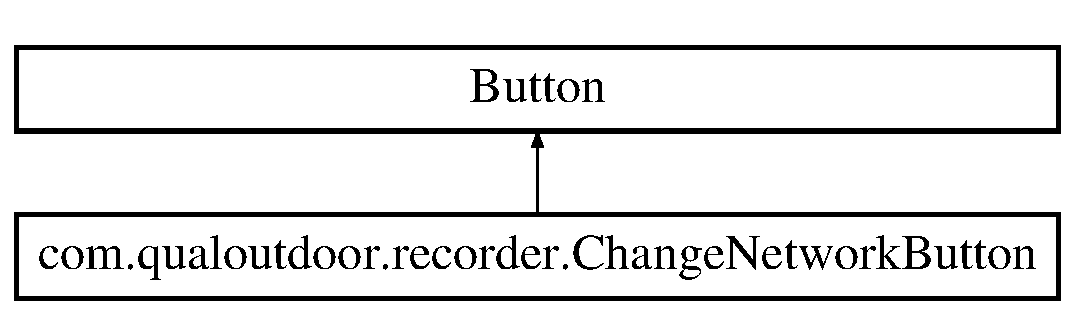
\includegraphics[height=2.000000cm]{classcom_1_1qualoutdoor_1_1recorder_1_1ChangeNetworkButton}
\end{center}
\end{figure}
\subsection*{Public Member Functions}
\begin{DoxyCompactItemize}
\item 
\hypertarget{classcom_1_1qualoutdoor_1_1recorder_1_1ChangeNetworkButton_a1ec861ea067b2f79202f8c2d10a8549b}{{\bfseries Change\-Network\-Button} (Context context)}\label{classcom_1_1qualoutdoor_1_1recorder_1_1ChangeNetworkButton_a1ec861ea067b2f79202f8c2d10a8549b}

\item 
\hypertarget{classcom_1_1qualoutdoor_1_1recorder_1_1ChangeNetworkButton_aa5a17b922a1d5b972f13b6c4574af988}{{\bfseries Change\-Network\-Button} (Context context, Attribute\-Set attrs, int def\-Style)}\label{classcom_1_1qualoutdoor_1_1recorder_1_1ChangeNetworkButton_aa5a17b922a1d5b972f13b6c4574af988}

\item 
\hypertarget{classcom_1_1qualoutdoor_1_1recorder_1_1ChangeNetworkButton_a0663b052f5164177b6c7e9de01183e35}{{\bfseries Change\-Network\-Button} (Context context, Attribute\-Set attrs)}\label{classcom_1_1qualoutdoor_1_1recorder_1_1ChangeNetworkButton_a0663b052f5164177b6c7e9de01183e35}

\end{DoxyCompactItemize}
\subsection*{Protected Member Functions}
\begin{DoxyCompactItemize}
\item 
\hypertarget{classcom_1_1qualoutdoor_1_1recorder_1_1ChangeNetworkButton_a6a178a0b36b9f27facbb7b591778424c}{void {\bfseries on\-Attached\-To\-Window} ()}\label{classcom_1_1qualoutdoor_1_1recorder_1_1ChangeNetworkButton_a6a178a0b36b9f27facbb7b591778424c}

\end{DoxyCompactItemize}
\subsection*{Private Member Functions}
\begin{DoxyCompactItemize}
\item 
void \hyperlink{classcom_1_1qualoutdoor_1_1recorder_1_1ChangeNetworkButton_a1455cadd6a3ad0cc1a8e2fbcce388bb5}{action\-Change\-Network} (View view)
\end{DoxyCompactItemize}


\subsection{Detailed Description}


Definition at line 11 of file Change\-Network\-Button.\-java.



\subsection{Member Function Documentation}
\hypertarget{classcom_1_1qualoutdoor_1_1recorder_1_1ChangeNetworkButton_a1455cadd6a3ad0cc1a8e2fbcce388bb5}{\index{com\-::qualoutdoor\-::recorder\-::\-Change\-Network\-Button@{com\-::qualoutdoor\-::recorder\-::\-Change\-Network\-Button}!action\-Change\-Network@{action\-Change\-Network}}
\index{action\-Change\-Network@{action\-Change\-Network}!com::qualoutdoor::recorder::ChangeNetworkButton@{com\-::qualoutdoor\-::recorder\-::\-Change\-Network\-Button}}
\subsubsection[{action\-Change\-Network}]{\setlength{\rightskip}{0pt plus 5cm}void com.\-qualoutdoor.\-recorder.\-Change\-Network\-Button.\-action\-Change\-Network (
\begin{DoxyParamCaption}
\item[{View}]{view}
\end{DoxyParamCaption}
)\hspace{0.3cm}{\ttfamily [private]}}}\label{classcom_1_1qualoutdoor_1_1recorder_1_1ChangeNetworkButton_a1455cadd6a3ad0cc1a8e2fbcce388bb5}
Change the current network artificially 

Definition at line 42 of file Change\-Network\-Button.\-java.



The documentation for this class was generated from the following file\-:\begin{DoxyCompactItemize}
\item 
src/com/qualoutdoor/recorder/Change\-Network\-Button.\-java\end{DoxyCompactItemize}

\hypertarget{classcom_1_1qualoutdoor_1_1recorder_1_1map_1_1ColoredScale}{\section{com.\-qualoutdoor.\-recorder.\-map.\-Colored\-Scale Class Reference}
\label{classcom_1_1qualoutdoor_1_1recorder_1_1map_1_1ColoredScale}\index{com.\-qualoutdoor.\-recorder.\-map.\-Colored\-Scale@{com.\-qualoutdoor.\-recorder.\-map.\-Colored\-Scale}}
}
Inheritance diagram for com.\-qualoutdoor.\-recorder.\-map.\-Colored\-Scale\-:\begin{figure}[H]
\begin{center}
\leavevmode
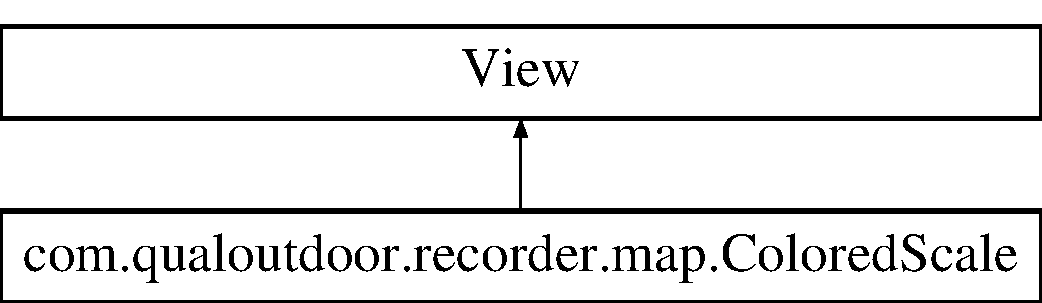
\includegraphics[height=2.000000cm]{classcom_1_1qualoutdoor_1_1recorder_1_1map_1_1ColoredScale}
\end{center}
\end{figure}
\subsection*{Public Member Functions}
\begin{DoxyCompactItemize}
\item 
\hyperlink{classcom_1_1qualoutdoor_1_1recorder_1_1map_1_1ColoredScale_aa55ac3d9ba5be9d14840830681e52e2d}{Colored\-Scale} (Context context)
\item 
\hyperlink{classcom_1_1qualoutdoor_1_1recorder_1_1map_1_1ColoredScale_ab945cb4bff3bb2bc529197fc9c7ed3d5}{Colored\-Scale} (Context context, Attribute\-Set attrs)
\item 
boolean \hyperlink{classcom_1_1qualoutdoor_1_1recorder_1_1map_1_1ColoredScale_a4fea7eb8fd4576d8ccafea91515848b1}{get\-Show\-Text} ()
\item 
void \hyperlink{classcom_1_1qualoutdoor_1_1recorder_1_1map_1_1ColoredScale_a5e8e2c07ea98d8583ada6ce92c69f789}{set\-Show\-Text} (boolean show\-Text)
\item 
float \hyperlink{classcom_1_1qualoutdoor_1_1recorder_1_1map_1_1ColoredScale_a3244dd95dd06a4d1ae7dd73f95509022}{get\-Text\-Y} ()
\item 
void \hyperlink{classcom_1_1qualoutdoor_1_1recorder_1_1map_1_1ColoredScale_a4f0ee3e627c89804b6e99cce9a7ca837}{set\-Text\-Y} (float text\-Y)
\item 
float \hyperlink{classcom_1_1qualoutdoor_1_1recorder_1_1map_1_1ColoredScale_a0f4b620c63df88430c1bf482872b4f38}{get\-Text\-Width} ()
\item 
void \hyperlink{classcom_1_1qualoutdoor_1_1recorder_1_1map_1_1ColoredScale_ad271444a49aeb6230a5f60321826f9b4}{set\-Text\-Width} (float text\-Width)
\item 
float \hyperlink{classcom_1_1qualoutdoor_1_1recorder_1_1map_1_1ColoredScale_a1c6d7f61f9909fd3d35e12f9c9dfa03a}{get\-Text\-Height} ()
\item 
void \hyperlink{classcom_1_1qualoutdoor_1_1recorder_1_1map_1_1ColoredScale_aaebda524aa8726568f1055e31777dece}{set\-Text\-Height} (float text\-Height)
\end{DoxyCompactItemize}
\subsection*{Protected Member Functions}
\begin{DoxyCompactItemize}
\item 
\hypertarget{classcom_1_1qualoutdoor_1_1recorder_1_1map_1_1ColoredScale_a80ca17312e54ae5d8e74c4bdf6d5253a}{void {\bfseries on\-Size\-Changed} (int w, int h, int oldw, int oldh)}\label{classcom_1_1qualoutdoor_1_1recorder_1_1map_1_1ColoredScale_a80ca17312e54ae5d8e74c4bdf6d5253a}

\item 
\hypertarget{classcom_1_1qualoutdoor_1_1recorder_1_1map_1_1ColoredScale_a0b8692a3eed077a960f18ad4a9b04798}{void {\bfseries on\-Draw} (Canvas canvas)}\label{classcom_1_1qualoutdoor_1_1recorder_1_1map_1_1ColoredScale_a0b8692a3eed077a960f18ad4a9b04798}

\item 
\hypertarget{classcom_1_1qualoutdoor_1_1recorder_1_1map_1_1ColoredScale_a79be240a4bfba2b93b88df71ef1035b9}{int {\bfseries get\-Suggested\-Minimum\-Height} ()}\label{classcom_1_1qualoutdoor_1_1recorder_1_1map_1_1ColoredScale_a79be240a4bfba2b93b88df71ef1035b9}

\item 
\hypertarget{classcom_1_1qualoutdoor_1_1recorder_1_1map_1_1ColoredScale_a05edef11c21f7dc8aab2c98944c52372}{void {\bfseries on\-Measure} (int width\-Measure\-Spec, int height\-Measure\-Spec)}\label{classcom_1_1qualoutdoor_1_1recorder_1_1map_1_1ColoredScale_a05edef11c21f7dc8aab2c98944c52372}

\end{DoxyCompactItemize}
\subsection*{Private Member Functions}
\begin{DoxyCompactItemize}
\item 
void \hyperlink{classcom_1_1qualoutdoor_1_1recorder_1_1map_1_1ColoredScale_a2e15ef8de5c135bc1967e33d7a0095a5}{init} ()
\item 
int \hyperlink{classcom_1_1qualoutdoor_1_1recorder_1_1map_1_1ColoredScale_a497e3a7f1dd45ff848916b04d31c4e7d}{compatible\-Resolve\-Size\-And\-State} (int size, int measure\-Spec, int child\-Measured\-State)
\end{DoxyCompactItemize}
\subsection*{Private Attributes}
\begin{DoxyCompactItemize}
\item 
\hypertarget{classcom_1_1qualoutdoor_1_1recorder_1_1map_1_1ColoredScale_a587907917914f0d1ec452a367a327a70}{String {\bfseries m\-Text}}\label{classcom_1_1qualoutdoor_1_1recorder_1_1map_1_1ColoredScale_a587907917914f0d1ec452a367a327a70}

\item 
int \hyperlink{classcom_1_1qualoutdoor_1_1recorder_1_1map_1_1ColoredScale_ad44c4a8f10141db919a6c1f023200b6f}{m\-Text\-Color}
\item 
float \hyperlink{classcom_1_1qualoutdoor_1_1recorder_1_1map_1_1ColoredScale_a4188abd3292c87be882a40a1adc507d1}{m\-Start\-Value}
\item 
float \hyperlink{classcom_1_1qualoutdoor_1_1recorder_1_1map_1_1ColoredScale_a5b5033b8ddba63337370fd55a33606da}{m\-End\-Value}
\item 
float \hyperlink{classcom_1_1qualoutdoor_1_1recorder_1_1map_1_1ColoredScale_a37da9656dfcfcfa61978d4f4689be5e3}{m\-Graduation\-Step}
\item 
int \hyperlink{classcom_1_1qualoutdoor_1_1recorder_1_1map_1_1ColoredScale_a6cf7926b347e1eed939659ea7f1bd320}{m\-Start\-Color}
\item 
int \hyperlink{classcom_1_1qualoutdoor_1_1recorder_1_1map_1_1ColoredScale_abf24fe5c047b605e6e295dd547046cea}{m\-End\-Color}
\item 
int \hyperlink{classcom_1_1qualoutdoor_1_1recorder_1_1map_1_1ColoredScale_a1620990b3e64cb7cf4d629e035779e6c}{m\-Graduation\-Start\-Color}
\item 
int \hyperlink{classcom_1_1qualoutdoor_1_1recorder_1_1map_1_1ColoredScale_a1da3cc13ab28d256b0db3abf714d035a}{m\-Graduation\-End\-Color}
\item 
Paint \hyperlink{classcom_1_1qualoutdoor_1_1recorder_1_1map_1_1ColoredScale_a7947eab323f541a31cd1b0eee694aa3d}{m\-Scale\-Paint}
\item 
Paint \hyperlink{classcom_1_1qualoutdoor_1_1recorder_1_1map_1_1ColoredScale_af3daf806f487c61997e7b16f3f49aa3c}{m\-Graduation\-Paint}
\item 
Paint \hyperlink{classcom_1_1qualoutdoor_1_1recorder_1_1map_1_1ColoredScale_ace9a89e3cf770b47b0f474eca3c8b503}{m\-Text\-Paint}
\item 
boolean \hyperlink{classcom_1_1qualoutdoor_1_1recorder_1_1map_1_1ColoredScale_aa9cb5cdbc2354b01553207fc9ea9015a}{m\-Show\-Text} = false
\item 
float \hyperlink{classcom_1_1qualoutdoor_1_1recorder_1_1map_1_1ColoredScale_a84b3e55223428d8643cec8188439e531}{m\-Text\-X} = 0.\-0f
\item 
float \hyperlink{classcom_1_1qualoutdoor_1_1recorder_1_1map_1_1ColoredScale_ab569fbf05d637f90977cc654ceea7347}{m\-Text\-Y} = 0.\-0f
\item 
float \hyperlink{classcom_1_1qualoutdoor_1_1recorder_1_1map_1_1ColoredScale_a6b2b1664c8d9e81e37aea2a092938f90}{m\-Text\-Width} = 0.\-0f
\item 
float \hyperlink{classcom_1_1qualoutdoor_1_1recorder_1_1map_1_1ColoredScale_a86eef0d17d57905f4816680963300ca3}{m\-Text\-Height} = 0.\-0f
\item 
float \hyperlink{classcom_1_1qualoutdoor_1_1recorder_1_1map_1_1ColoredScale_a58b6c932c202e2187af22aeb947f1e23}{m\-Graduation\-Length}
\item 
Rect\-F \hyperlink{classcom_1_1qualoutdoor_1_1recorder_1_1map_1_1ColoredScale_adcbf03acb4ab5e83cdf1d0e3bb3dc900}{m\-Scale\-Rect} = new Rect\-F()
\end{DoxyCompactItemize}


\subsection{Detailed Description}


Definition at line 16 of file Colored\-Scale.\-java.



\subsection{Constructor \& Destructor Documentation}
\hypertarget{classcom_1_1qualoutdoor_1_1recorder_1_1map_1_1ColoredScale_aa55ac3d9ba5be9d14840830681e52e2d}{\index{com\-::qualoutdoor\-::recorder\-::map\-::\-Colored\-Scale@{com\-::qualoutdoor\-::recorder\-::map\-::\-Colored\-Scale}!Colored\-Scale@{Colored\-Scale}}
\index{Colored\-Scale@{Colored\-Scale}!com::qualoutdoor::recorder::map::ColoredScale@{com\-::qualoutdoor\-::recorder\-::map\-::\-Colored\-Scale}}
\subsubsection[{Colored\-Scale}]{\setlength{\rightskip}{0pt plus 5cm}com.\-qualoutdoor.\-recorder.\-map.\-Colored\-Scale.\-Colored\-Scale (
\begin{DoxyParamCaption}
\item[{Context}]{context}
\end{DoxyParamCaption}
)}}\label{classcom_1_1qualoutdoor_1_1recorder_1_1map_1_1ColoredScale_aa55ac3d9ba5be9d14840830681e52e2d}
$<$ The boundaries of the scale itself Class constructor taking only a context. Use this constructor to create \hyperlink{classcom_1_1qualoutdoor_1_1recorder_1_1map_1_1ColoredScale}{Colored\-Scale} objects from your own code.


\begin{DoxyParams}{Parameters}
{\em context} & \\
\hline
\end{DoxyParams}


Definition at line 73 of file Colored\-Scale.\-java.



References com.\-qualoutdoor.\-recorder.\-map.\-Colored\-Scale.\-init().

\hypertarget{classcom_1_1qualoutdoor_1_1recorder_1_1map_1_1ColoredScale_ab945cb4bff3bb2bc529197fc9c7ed3d5}{\index{com\-::qualoutdoor\-::recorder\-::map\-::\-Colored\-Scale@{com\-::qualoutdoor\-::recorder\-::map\-::\-Colored\-Scale}!Colored\-Scale@{Colored\-Scale}}
\index{Colored\-Scale@{Colored\-Scale}!com::qualoutdoor::recorder::map::ColoredScale@{com\-::qualoutdoor\-::recorder\-::map\-::\-Colored\-Scale}}
\subsubsection[{Colored\-Scale}]{\setlength{\rightskip}{0pt plus 5cm}com.\-qualoutdoor.\-recorder.\-map.\-Colored\-Scale.\-Colored\-Scale (
\begin{DoxyParamCaption}
\item[{Context}]{context, }
\item[{Attribute\-Set}]{attrs}
\end{DoxyParamCaption}
)}}\label{classcom_1_1qualoutdoor_1_1recorder_1_1map_1_1ColoredScale_ab945cb4bff3bb2bc529197fc9c7ed3d5}
Class constructor taking a context and an attribute set. This constructor is used by the layout engine to construct a \hyperlink{classcom_1_1qualoutdoor_1_1recorder_1_1map_1_1ColoredScale}{Colored\-Scale} from a set of X\-M\-L attributes.


\begin{DoxyParams}{Parameters}
{\em context} & \\
\hline
{\em attrs} & An attribute set which can contain attributes from \hyperlink{}{R.\-styleable.\-Colored\-Scale} as well as attributes inherited from \hyperlink{}{android.\-view.\-View}. \\
\hline
\end{DoxyParams}


Definition at line 89 of file Colored\-Scale.\-java.



References com.\-qualoutdoor.\-recorder.\-map.\-Colored\-Scale.\-init(), com.\-qualoutdoor.\-recorder.\-map.\-Colored\-Scale.\-m\-End\-Color, com.\-qualoutdoor.\-recorder.\-map.\-Colored\-Scale.\-m\-End\-Value, com.\-qualoutdoor.\-recorder.\-map.\-Colored\-Scale.\-m\-Graduation\-End\-Color, com.\-qualoutdoor.\-recorder.\-map.\-Colored\-Scale.\-m\-Graduation\-Start\-Color, com.\-qualoutdoor.\-recorder.\-map.\-Colored\-Scale.\-m\-Graduation\-Step, com.\-qualoutdoor.\-recorder.\-map.\-Colored\-Scale.\-m\-Show\-Text, com.\-qualoutdoor.\-recorder.\-map.\-Colored\-Scale.\-m\-Start\-Color, com.\-qualoutdoor.\-recorder.\-map.\-Colored\-Scale.\-m\-Start\-Value, com.\-qualoutdoor.\-recorder.\-map.\-Colored\-Scale.\-m\-Text\-Color, and com.\-qualoutdoor.\-recorder.\-map.\-Colored\-Scale.\-m\-Text\-Height.



\subsection{Member Function Documentation}
\hypertarget{classcom_1_1qualoutdoor_1_1recorder_1_1map_1_1ColoredScale_a497e3a7f1dd45ff848916b04d31c4e7d}{\index{com\-::qualoutdoor\-::recorder\-::map\-::\-Colored\-Scale@{com\-::qualoutdoor\-::recorder\-::map\-::\-Colored\-Scale}!compatible\-Resolve\-Size\-And\-State@{compatible\-Resolve\-Size\-And\-State}}
\index{compatible\-Resolve\-Size\-And\-State@{compatible\-Resolve\-Size\-And\-State}!com::qualoutdoor::recorder::map::ColoredScale@{com\-::qualoutdoor\-::recorder\-::map\-::\-Colored\-Scale}}
\subsubsection[{compatible\-Resolve\-Size\-And\-State}]{\setlength{\rightskip}{0pt plus 5cm}int com.\-qualoutdoor.\-recorder.\-map.\-Colored\-Scale.\-compatible\-Resolve\-Size\-And\-State (
\begin{DoxyParamCaption}
\item[{int}]{size, }
\item[{int}]{measure\-Spec, }
\item[{int}]{child\-Measured\-State}
\end{DoxyParamCaption}
)\hspace{0.3cm}{\ttfamily [private]}}}\label{classcom_1_1qualoutdoor_1_1recorder_1_1map_1_1ColoredScale_a497e3a7f1dd45ff848916b04d31c4e7d}
Utility to reconcile a desired size and state, with constraints imposed by a Measure\-Spec. The original resolve\-Size\-And\-State requires A\-P\-I lvl 11. This version is meant to replace it for older version.


\begin{DoxyParams}{Parameters}
{\em size} & How big the view wants to be \\
\hline
{\em measure\-Spec} & Constraints imposed by the parent \\
\hline
{\em child\-Measured\-State} & \\
\hline
\end{DoxyParams}
\begin{DoxyReturn}{Returns}
Size information bit mask as defined by M\-E\-A\-S\-U\-R\-E\-D\-\_\-\-S\-I\-Z\-E\-\_\-\-M\-A\-S\-K and M\-E\-A\-S\-U\-R\-E\-D\-\_\-\-S\-T\-A\-T\-E\-\_\-\-T\-O\-O\-\_\-\-S\-M\-A\-L\-L. 
\end{DoxyReturn}


Definition at line 399 of file Colored\-Scale.\-java.

\hypertarget{classcom_1_1qualoutdoor_1_1recorder_1_1map_1_1ColoredScale_a4fea7eb8fd4576d8ccafea91515848b1}{\index{com\-::qualoutdoor\-::recorder\-::map\-::\-Colored\-Scale@{com\-::qualoutdoor\-::recorder\-::map\-::\-Colored\-Scale}!get\-Show\-Text@{get\-Show\-Text}}
\index{get\-Show\-Text@{get\-Show\-Text}!com::qualoutdoor::recorder::map::ColoredScale@{com\-::qualoutdoor\-::recorder\-::map\-::\-Colored\-Scale}}
\subsubsection[{get\-Show\-Text}]{\setlength{\rightskip}{0pt plus 5cm}boolean com.\-qualoutdoor.\-recorder.\-map.\-Colored\-Scale.\-get\-Show\-Text (
\begin{DoxyParamCaption}
{}
\end{DoxyParamCaption}
)}}\label{classcom_1_1qualoutdoor_1_1recorder_1_1map_1_1ColoredScale_a4fea7eb8fd4576d8ccafea91515848b1}
Returns true if the text label should be visible.

\begin{DoxyReturn}{Returns}
True if the text label should be visible, false otherwise. 
\end{DoxyReturn}


Definition at line 169 of file Colored\-Scale.\-java.



References com.\-qualoutdoor.\-recorder.\-map.\-Colored\-Scale.\-m\-Show\-Text.

\hypertarget{classcom_1_1qualoutdoor_1_1recorder_1_1map_1_1ColoredScale_a1c6d7f61f9909fd3d35e12f9c9dfa03a}{\index{com\-::qualoutdoor\-::recorder\-::map\-::\-Colored\-Scale@{com\-::qualoutdoor\-::recorder\-::map\-::\-Colored\-Scale}!get\-Text\-Height@{get\-Text\-Height}}
\index{get\-Text\-Height@{get\-Text\-Height}!com::qualoutdoor::recorder::map::ColoredScale@{com\-::qualoutdoor\-::recorder\-::map\-::\-Colored\-Scale}}
\subsubsection[{get\-Text\-Height}]{\setlength{\rightskip}{0pt plus 5cm}float com.\-qualoutdoor.\-recorder.\-map.\-Colored\-Scale.\-get\-Text\-Height (
\begin{DoxyParamCaption}
{}
\end{DoxyParamCaption}
)}}\label{classcom_1_1qualoutdoor_1_1recorder_1_1map_1_1ColoredScale_a1c6d7f61f9909fd3d35e12f9c9dfa03a}
Returns the height of the label font, in pixels.

\begin{DoxyReturn}{Returns}
The height of the label font, in pixels. 
\end{DoxyReturn}


Definition at line 236 of file Colored\-Scale.\-java.



References com.\-qualoutdoor.\-recorder.\-map.\-Colored\-Scale.\-m\-Text\-Height.

\hypertarget{classcom_1_1qualoutdoor_1_1recorder_1_1map_1_1ColoredScale_a0f4b620c63df88430c1bf482872b4f38}{\index{com\-::qualoutdoor\-::recorder\-::map\-::\-Colored\-Scale@{com\-::qualoutdoor\-::recorder\-::map\-::\-Colored\-Scale}!get\-Text\-Width@{get\-Text\-Width}}
\index{get\-Text\-Width@{get\-Text\-Width}!com::qualoutdoor::recorder::map::ColoredScale@{com\-::qualoutdoor\-::recorder\-::map\-::\-Colored\-Scale}}
\subsubsection[{get\-Text\-Width}]{\setlength{\rightskip}{0pt plus 5cm}float com.\-qualoutdoor.\-recorder.\-map.\-Colored\-Scale.\-get\-Text\-Width (
\begin{DoxyParamCaption}
{}
\end{DoxyParamCaption}
)}}\label{classcom_1_1qualoutdoor_1_1recorder_1_1map_1_1ColoredScale_a0f4b620c63df88430c1bf482872b4f38}
Returns the width reserved for label text, in pixels.

\begin{DoxyReturn}{Returns}
The width reserved for label text, in pixels. 
\end{DoxyReturn}


Definition at line 213 of file Colored\-Scale.\-java.



References com.\-qualoutdoor.\-recorder.\-map.\-Colored\-Scale.\-m\-Text\-Width.

\hypertarget{classcom_1_1qualoutdoor_1_1recorder_1_1map_1_1ColoredScale_a3244dd95dd06a4d1ae7dd73f95509022}{\index{com\-::qualoutdoor\-::recorder\-::map\-::\-Colored\-Scale@{com\-::qualoutdoor\-::recorder\-::map\-::\-Colored\-Scale}!get\-Text\-Y@{get\-Text\-Y}}
\index{get\-Text\-Y@{get\-Text\-Y}!com::qualoutdoor::recorder::map::ColoredScale@{com\-::qualoutdoor\-::recorder\-::map\-::\-Colored\-Scale}}
\subsubsection[{get\-Text\-Y}]{\setlength{\rightskip}{0pt plus 5cm}float com.\-qualoutdoor.\-recorder.\-map.\-Colored\-Scale.\-get\-Text\-Y (
\begin{DoxyParamCaption}
{}
\end{DoxyParamCaption}
)}}\label{classcom_1_1qualoutdoor_1_1recorder_1_1map_1_1ColoredScale_a3244dd95dd06a4d1ae7dd73f95509022}
Returns the Y position of the label text, in pixels.

\begin{DoxyReturn}{Returns}
The Y position of the label text, in pixels. 
\end{DoxyReturn}


Definition at line 192 of file Colored\-Scale.\-java.



References com.\-qualoutdoor.\-recorder.\-map.\-Colored\-Scale.\-m\-Text\-Y.

\hypertarget{classcom_1_1qualoutdoor_1_1recorder_1_1map_1_1ColoredScale_a2e15ef8de5c135bc1967e33d7a0095a5}{\index{com\-::qualoutdoor\-::recorder\-::map\-::\-Colored\-Scale@{com\-::qualoutdoor\-::recorder\-::map\-::\-Colored\-Scale}!init@{init}}
\index{init@{init}!com::qualoutdoor::recorder::map::ColoredScale@{com\-::qualoutdoor\-::recorder\-::map\-::\-Colored\-Scale}}
\subsubsection[{init}]{\setlength{\rightskip}{0pt plus 5cm}void com.\-qualoutdoor.\-recorder.\-map.\-Colored\-Scale.\-init (
\begin{DoxyParamCaption}
{}
\end{DoxyParamCaption}
)\hspace{0.3cm}{\ttfamily [private]}}}\label{classcom_1_1qualoutdoor_1_1recorder_1_1map_1_1ColoredScale_a2e15ef8de5c135bc1967e33d7a0095a5}
Initialize some size independant attributes. This code is in a separate method so that it can be called from both constructors. 

Definition at line 142 of file Colored\-Scale.\-java.



References com.\-qualoutdoor.\-recorder.\-map.\-Colored\-Scale.\-m\-Graduation\-Paint, com.\-qualoutdoor.\-recorder.\-map.\-Colored\-Scale.\-m\-Scale\-Paint, com.\-qualoutdoor.\-recorder.\-map.\-Colored\-Scale.\-m\-Text\-Color, com.\-qualoutdoor.\-recorder.\-map.\-Colored\-Scale.\-m\-Text\-Height, and com.\-qualoutdoor.\-recorder.\-map.\-Colored\-Scale.\-m\-Text\-Paint.



Referenced by com.\-qualoutdoor.\-recorder.\-map.\-Colored\-Scale.\-Colored\-Scale().

\hypertarget{classcom_1_1qualoutdoor_1_1recorder_1_1map_1_1ColoredScale_a5e8e2c07ea98d8583ada6ce92c69f789}{\index{com\-::qualoutdoor\-::recorder\-::map\-::\-Colored\-Scale@{com\-::qualoutdoor\-::recorder\-::map\-::\-Colored\-Scale}!set\-Show\-Text@{set\-Show\-Text}}
\index{set\-Show\-Text@{set\-Show\-Text}!com::qualoutdoor::recorder::map::ColoredScale@{com\-::qualoutdoor\-::recorder\-::map\-::\-Colored\-Scale}}
\subsubsection[{set\-Show\-Text}]{\setlength{\rightskip}{0pt plus 5cm}void com.\-qualoutdoor.\-recorder.\-map.\-Colored\-Scale.\-set\-Show\-Text (
\begin{DoxyParamCaption}
\item[{boolean}]{show\-Text}
\end{DoxyParamCaption}
)}}\label{classcom_1_1qualoutdoor_1_1recorder_1_1map_1_1ColoredScale_a5e8e2c07ea98d8583ada6ce92c69f789}
Controls whether the text label is visible or not. Setting this property to false allows the colored scale graphic to take up the entire visible area of the control.


\begin{DoxyParams}{Parameters}
{\em show\-Text} & true if the text label should be visible, false otherwise \\
\hline
\end{DoxyParams}


Definition at line 181 of file Colored\-Scale.\-java.



References com.\-qualoutdoor.\-recorder.\-map.\-Colored\-Scale.\-m\-Show\-Text.

\hypertarget{classcom_1_1qualoutdoor_1_1recorder_1_1map_1_1ColoredScale_aaebda524aa8726568f1055e31777dece}{\index{com\-::qualoutdoor\-::recorder\-::map\-::\-Colored\-Scale@{com\-::qualoutdoor\-::recorder\-::map\-::\-Colored\-Scale}!set\-Text\-Height@{set\-Text\-Height}}
\index{set\-Text\-Height@{set\-Text\-Height}!com::qualoutdoor::recorder::map::ColoredScale@{com\-::qualoutdoor\-::recorder\-::map\-::\-Colored\-Scale}}
\subsubsection[{set\-Text\-Height}]{\setlength{\rightskip}{0pt plus 5cm}void com.\-qualoutdoor.\-recorder.\-map.\-Colored\-Scale.\-set\-Text\-Height (
\begin{DoxyParamCaption}
\item[{float}]{text\-Height}
\end{DoxyParamCaption}
)}}\label{classcom_1_1qualoutdoor_1_1recorder_1_1map_1_1ColoredScale_aaebda524aa8726568f1055e31777dece}
Set the height of the label font, in pixels.


\begin{DoxyParams}{Parameters}
{\em text\-Height} & The height of the label font, in pixels. \\
\hline
\end{DoxyParams}


Definition at line 246 of file Colored\-Scale.\-java.



References com.\-qualoutdoor.\-recorder.\-map.\-Colored\-Scale.\-m\-Text\-Height.

\hypertarget{classcom_1_1qualoutdoor_1_1recorder_1_1map_1_1ColoredScale_ad271444a49aeb6230a5f60321826f9b4}{\index{com\-::qualoutdoor\-::recorder\-::map\-::\-Colored\-Scale@{com\-::qualoutdoor\-::recorder\-::map\-::\-Colored\-Scale}!set\-Text\-Width@{set\-Text\-Width}}
\index{set\-Text\-Width@{set\-Text\-Width}!com::qualoutdoor::recorder::map::ColoredScale@{com\-::qualoutdoor\-::recorder\-::map\-::\-Colored\-Scale}}
\subsubsection[{set\-Text\-Width}]{\setlength{\rightskip}{0pt plus 5cm}void com.\-qualoutdoor.\-recorder.\-map.\-Colored\-Scale.\-set\-Text\-Width (
\begin{DoxyParamCaption}
\item[{float}]{text\-Width}
\end{DoxyParamCaption}
)}}\label{classcom_1_1qualoutdoor_1_1recorder_1_1map_1_1ColoredScale_ad271444a49aeb6230a5f60321826f9b4}
Set the width of the area reserved for label text. This width is constant; it does not change based on the actual width of the label as the label text changes.


\begin{DoxyParams}{Parameters}
{\em text\-Width} & The width reserved for label text, in pixels. \\
\hline
\end{DoxyParams}


Definition at line 225 of file Colored\-Scale.\-java.



References com.\-qualoutdoor.\-recorder.\-map.\-Colored\-Scale.\-m\-Text\-Width.

\hypertarget{classcom_1_1qualoutdoor_1_1recorder_1_1map_1_1ColoredScale_a4f0ee3e627c89804b6e99cce9a7ca837}{\index{com\-::qualoutdoor\-::recorder\-::map\-::\-Colored\-Scale@{com\-::qualoutdoor\-::recorder\-::map\-::\-Colored\-Scale}!set\-Text\-Y@{set\-Text\-Y}}
\index{set\-Text\-Y@{set\-Text\-Y}!com::qualoutdoor::recorder::map::ColoredScale@{com\-::qualoutdoor\-::recorder\-::map\-::\-Colored\-Scale}}
\subsubsection[{set\-Text\-Y}]{\setlength{\rightskip}{0pt plus 5cm}void com.\-qualoutdoor.\-recorder.\-map.\-Colored\-Scale.\-set\-Text\-Y (
\begin{DoxyParamCaption}
\item[{float}]{text\-Y}
\end{DoxyParamCaption}
)}}\label{classcom_1_1qualoutdoor_1_1recorder_1_1map_1_1ColoredScale_a4f0ee3e627c89804b6e99cce9a7ca837}
Set the Y position of the label text, in pixels.


\begin{DoxyParams}{Parameters}
{\em text\-Y} & the Y position of the label text, in pixels. \\
\hline
\end{DoxyParams}


Definition at line 202 of file Colored\-Scale.\-java.



References com.\-qualoutdoor.\-recorder.\-map.\-Colored\-Scale.\-m\-Text\-Y.



\subsection{Member Data Documentation}
\hypertarget{classcom_1_1qualoutdoor_1_1recorder_1_1map_1_1ColoredScale_abf24fe5c047b605e6e295dd547046cea}{\index{com\-::qualoutdoor\-::recorder\-::map\-::\-Colored\-Scale@{com\-::qualoutdoor\-::recorder\-::map\-::\-Colored\-Scale}!m\-End\-Color@{m\-End\-Color}}
\index{m\-End\-Color@{m\-End\-Color}!com::qualoutdoor::recorder::map::ColoredScale@{com\-::qualoutdoor\-::recorder\-::map\-::\-Colored\-Scale}}
\subsubsection[{m\-End\-Color}]{\setlength{\rightskip}{0pt plus 5cm}int com.\-qualoutdoor.\-recorder.\-map.\-Colored\-Scale.\-m\-End\-Color\hspace{0.3cm}{\ttfamily [private]}}}\label{classcom_1_1qualoutdoor_1_1recorder_1_1map_1_1ColoredScale_abf24fe5c047b605e6e295dd547046cea}
$<$ The starting color of the scale 

Definition at line 32 of file Colored\-Scale.\-java.



Referenced by com.\-qualoutdoor.\-recorder.\-map.\-Colored\-Scale.\-Colored\-Scale().

\hypertarget{classcom_1_1qualoutdoor_1_1recorder_1_1map_1_1ColoredScale_a5b5033b8ddba63337370fd55a33606da}{\index{com\-::qualoutdoor\-::recorder\-::map\-::\-Colored\-Scale@{com\-::qualoutdoor\-::recorder\-::map\-::\-Colored\-Scale}!m\-End\-Value@{m\-End\-Value}}
\index{m\-End\-Value@{m\-End\-Value}!com::qualoutdoor::recorder::map::ColoredScale@{com\-::qualoutdoor\-::recorder\-::map\-::\-Colored\-Scale}}
\subsubsection[{m\-End\-Value}]{\setlength{\rightskip}{0pt plus 5cm}float com.\-qualoutdoor.\-recorder.\-map.\-Colored\-Scale.\-m\-End\-Value\hspace{0.3cm}{\ttfamily [private]}}}\label{classcom_1_1qualoutdoor_1_1recorder_1_1map_1_1ColoredScale_a5b5033b8ddba63337370fd55a33606da}
$<$ The minimum value of the scale 

Definition at line 25 of file Colored\-Scale.\-java.



Referenced by com.\-qualoutdoor.\-recorder.\-map.\-Colored\-Scale.\-Colored\-Scale().

\hypertarget{classcom_1_1qualoutdoor_1_1recorder_1_1map_1_1ColoredScale_a1da3cc13ab28d256b0db3abf714d035a}{\index{com\-::qualoutdoor\-::recorder\-::map\-::\-Colored\-Scale@{com\-::qualoutdoor\-::recorder\-::map\-::\-Colored\-Scale}!m\-Graduation\-End\-Color@{m\-Graduation\-End\-Color}}
\index{m\-Graduation\-End\-Color@{m\-Graduation\-End\-Color}!com::qualoutdoor::recorder::map::ColoredScale@{com\-::qualoutdoor\-::recorder\-::map\-::\-Colored\-Scale}}
\subsubsection[{m\-Graduation\-End\-Color}]{\setlength{\rightskip}{0pt plus 5cm}int com.\-qualoutdoor.\-recorder.\-map.\-Colored\-Scale.\-m\-Graduation\-End\-Color\hspace{0.3cm}{\ttfamily [private]}}}\label{classcom_1_1qualoutdoor_1_1recorder_1_1map_1_1ColoredScale_a1da3cc13ab28d256b0db3abf714d035a}
$<$ The starting color of the graduation lines 

Definition at line 37 of file Colored\-Scale.\-java.



Referenced by com.\-qualoutdoor.\-recorder.\-map.\-Colored\-Scale.\-Colored\-Scale().

\hypertarget{classcom_1_1qualoutdoor_1_1recorder_1_1map_1_1ColoredScale_a58b6c932c202e2187af22aeb947f1e23}{\index{com\-::qualoutdoor\-::recorder\-::map\-::\-Colored\-Scale@{com\-::qualoutdoor\-::recorder\-::map\-::\-Colored\-Scale}!m\-Graduation\-Length@{m\-Graduation\-Length}}
\index{m\-Graduation\-Length@{m\-Graduation\-Length}!com::qualoutdoor::recorder::map::ColoredScale@{com\-::qualoutdoor\-::recorder\-::map\-::\-Colored\-Scale}}
\subsubsection[{m\-Graduation\-Length}]{\setlength{\rightskip}{0pt plus 5cm}float com.\-qualoutdoor.\-recorder.\-map.\-Colored\-Scale.\-m\-Graduation\-Length\hspace{0.3cm}{\ttfamily [private]}}}\label{classcom_1_1qualoutdoor_1_1recorder_1_1map_1_1ColoredScale_a58b6c932c202e2187af22aeb947f1e23}
$<$ The height of the text label, in pixels 

Definition at line 60 of file Colored\-Scale.\-java.

\hypertarget{classcom_1_1qualoutdoor_1_1recorder_1_1map_1_1ColoredScale_af3daf806f487c61997e7b16f3f49aa3c}{\index{com\-::qualoutdoor\-::recorder\-::map\-::\-Colored\-Scale@{com\-::qualoutdoor\-::recorder\-::map\-::\-Colored\-Scale}!m\-Graduation\-Paint@{m\-Graduation\-Paint}}
\index{m\-Graduation\-Paint@{m\-Graduation\-Paint}!com::qualoutdoor::recorder::map::ColoredScale@{com\-::qualoutdoor\-::recorder\-::map\-::\-Colored\-Scale}}
\subsubsection[{m\-Graduation\-Paint}]{\setlength{\rightskip}{0pt plus 5cm}Paint com.\-qualoutdoor.\-recorder.\-map.\-Colored\-Scale.\-m\-Graduation\-Paint\hspace{0.3cm}{\ttfamily [private]}}}\label{classcom_1_1qualoutdoor_1_1recorder_1_1map_1_1ColoredScale_af3daf806f487c61997e7b16f3f49aa3c}
$<$ Paint that define the scale style 

Definition at line 42 of file Colored\-Scale.\-java.



Referenced by com.\-qualoutdoor.\-recorder.\-map.\-Colored\-Scale.\-init().

\hypertarget{classcom_1_1qualoutdoor_1_1recorder_1_1map_1_1ColoredScale_a1620990b3e64cb7cf4d629e035779e6c}{\index{com\-::qualoutdoor\-::recorder\-::map\-::\-Colored\-Scale@{com\-::qualoutdoor\-::recorder\-::map\-::\-Colored\-Scale}!m\-Graduation\-Start\-Color@{m\-Graduation\-Start\-Color}}
\index{m\-Graduation\-Start\-Color@{m\-Graduation\-Start\-Color}!com::qualoutdoor::recorder::map::ColoredScale@{com\-::qualoutdoor\-::recorder\-::map\-::\-Colored\-Scale}}
\subsubsection[{m\-Graduation\-Start\-Color}]{\setlength{\rightskip}{0pt plus 5cm}int com.\-qualoutdoor.\-recorder.\-map.\-Colored\-Scale.\-m\-Graduation\-Start\-Color\hspace{0.3cm}{\ttfamily [private]}}}\label{classcom_1_1qualoutdoor_1_1recorder_1_1map_1_1ColoredScale_a1620990b3e64cb7cf4d629e035779e6c}
$<$ The ending color of the scale 

Definition at line 35 of file Colored\-Scale.\-java.



Referenced by com.\-qualoutdoor.\-recorder.\-map.\-Colored\-Scale.\-Colored\-Scale().

\hypertarget{classcom_1_1qualoutdoor_1_1recorder_1_1map_1_1ColoredScale_a37da9656dfcfcfa61978d4f4689be5e3}{\index{com\-::qualoutdoor\-::recorder\-::map\-::\-Colored\-Scale@{com\-::qualoutdoor\-::recorder\-::map\-::\-Colored\-Scale}!m\-Graduation\-Step@{m\-Graduation\-Step}}
\index{m\-Graduation\-Step@{m\-Graduation\-Step}!com::qualoutdoor::recorder::map::ColoredScale@{com\-::qualoutdoor\-::recorder\-::map\-::\-Colored\-Scale}}
\subsubsection[{m\-Graduation\-Step}]{\setlength{\rightskip}{0pt plus 5cm}float com.\-qualoutdoor.\-recorder.\-map.\-Colored\-Scale.\-m\-Graduation\-Step\hspace{0.3cm}{\ttfamily [private]}}}\label{classcom_1_1qualoutdoor_1_1recorder_1_1map_1_1ColoredScale_a37da9656dfcfcfa61978d4f4689be5e3}
$<$ The maximum value of the scale 

Definition at line 27 of file Colored\-Scale.\-java.



Referenced by com.\-qualoutdoor.\-recorder.\-map.\-Colored\-Scale.\-Colored\-Scale().

\hypertarget{classcom_1_1qualoutdoor_1_1recorder_1_1map_1_1ColoredScale_a7947eab323f541a31cd1b0eee694aa3d}{\index{com\-::qualoutdoor\-::recorder\-::map\-::\-Colored\-Scale@{com\-::qualoutdoor\-::recorder\-::map\-::\-Colored\-Scale}!m\-Scale\-Paint@{m\-Scale\-Paint}}
\index{m\-Scale\-Paint@{m\-Scale\-Paint}!com::qualoutdoor::recorder::map::ColoredScale@{com\-::qualoutdoor\-::recorder\-::map\-::\-Colored\-Scale}}
\subsubsection[{m\-Scale\-Paint}]{\setlength{\rightskip}{0pt plus 5cm}Paint com.\-qualoutdoor.\-recorder.\-map.\-Colored\-Scale.\-m\-Scale\-Paint\hspace{0.3cm}{\ttfamily [private]}}}\label{classcom_1_1qualoutdoor_1_1recorder_1_1map_1_1ColoredScale_a7947eab323f541a31cd1b0eee694aa3d}
$<$ The ending color of the graduation lines 

Definition at line 40 of file Colored\-Scale.\-java.



Referenced by com.\-qualoutdoor.\-recorder.\-map.\-Colored\-Scale.\-init().

\hypertarget{classcom_1_1qualoutdoor_1_1recorder_1_1map_1_1ColoredScale_adcbf03acb4ab5e83cdf1d0e3bb3dc900}{\index{com\-::qualoutdoor\-::recorder\-::map\-::\-Colored\-Scale@{com\-::qualoutdoor\-::recorder\-::map\-::\-Colored\-Scale}!m\-Scale\-Rect@{m\-Scale\-Rect}}
\index{m\-Scale\-Rect@{m\-Scale\-Rect}!com::qualoutdoor::recorder::map::ColoredScale@{com\-::qualoutdoor\-::recorder\-::map\-::\-Colored\-Scale}}
\subsubsection[{m\-Scale\-Rect}]{\setlength{\rightskip}{0pt plus 5cm}Rect\-F com.\-qualoutdoor.\-recorder.\-map.\-Colored\-Scale.\-m\-Scale\-Rect = new Rect\-F()\hspace{0.3cm}{\ttfamily [private]}}}\label{classcom_1_1qualoutdoor_1_1recorder_1_1map_1_1ColoredScale_adcbf03acb4ab5e83cdf1d0e3bb3dc900}
$<$ The length of graduation lines 

Definition at line 63 of file Colored\-Scale.\-java.

\hypertarget{classcom_1_1qualoutdoor_1_1recorder_1_1map_1_1ColoredScale_aa9cb5cdbc2354b01553207fc9ea9015a}{\index{com\-::qualoutdoor\-::recorder\-::map\-::\-Colored\-Scale@{com\-::qualoutdoor\-::recorder\-::map\-::\-Colored\-Scale}!m\-Show\-Text@{m\-Show\-Text}}
\index{m\-Show\-Text@{m\-Show\-Text}!com::qualoutdoor::recorder::map::ColoredScale@{com\-::qualoutdoor\-::recorder\-::map\-::\-Colored\-Scale}}
\subsubsection[{m\-Show\-Text}]{\setlength{\rightskip}{0pt plus 5cm}boolean com.\-qualoutdoor.\-recorder.\-map.\-Colored\-Scale.\-m\-Show\-Text = false\hspace{0.3cm}{\ttfamily [private]}}}\label{classcom_1_1qualoutdoor_1_1recorder_1_1map_1_1ColoredScale_aa9cb5cdbc2354b01553207fc9ea9015a}
$<$ Paint that define the label style 

Definition at line 47 of file Colored\-Scale.\-java.



Referenced by com.\-qualoutdoor.\-recorder.\-map.\-Colored\-Scale.\-Colored\-Scale(), com.\-qualoutdoor.\-recorder.\-map.\-Colored\-Scale.\-get\-Show\-Text(), and com.\-qualoutdoor.\-recorder.\-map.\-Colored\-Scale.\-set\-Show\-Text().

\hypertarget{classcom_1_1qualoutdoor_1_1recorder_1_1map_1_1ColoredScale_a6cf7926b347e1eed939659ea7f1bd320}{\index{com\-::qualoutdoor\-::recorder\-::map\-::\-Colored\-Scale@{com\-::qualoutdoor\-::recorder\-::map\-::\-Colored\-Scale}!m\-Start\-Color@{m\-Start\-Color}}
\index{m\-Start\-Color@{m\-Start\-Color}!com::qualoutdoor::recorder::map::ColoredScale@{com\-::qualoutdoor\-::recorder\-::map\-::\-Colored\-Scale}}
\subsubsection[{m\-Start\-Color}]{\setlength{\rightskip}{0pt plus 5cm}int com.\-qualoutdoor.\-recorder.\-map.\-Colored\-Scale.\-m\-Start\-Color\hspace{0.3cm}{\ttfamily [private]}}}\label{classcom_1_1qualoutdoor_1_1recorder_1_1map_1_1ColoredScale_a6cf7926b347e1eed939659ea7f1bd320}
$<$ The precision of graduation 

Definition at line 30 of file Colored\-Scale.\-java.



Referenced by com.\-qualoutdoor.\-recorder.\-map.\-Colored\-Scale.\-Colored\-Scale().

\hypertarget{classcom_1_1qualoutdoor_1_1recorder_1_1map_1_1ColoredScale_a4188abd3292c87be882a40a1adc507d1}{\index{com\-::qualoutdoor\-::recorder\-::map\-::\-Colored\-Scale@{com\-::qualoutdoor\-::recorder\-::map\-::\-Colored\-Scale}!m\-Start\-Value@{m\-Start\-Value}}
\index{m\-Start\-Value@{m\-Start\-Value}!com::qualoutdoor::recorder::map::ColoredScale@{com\-::qualoutdoor\-::recorder\-::map\-::\-Colored\-Scale}}
\subsubsection[{m\-Start\-Value}]{\setlength{\rightskip}{0pt plus 5cm}float com.\-qualoutdoor.\-recorder.\-map.\-Colored\-Scale.\-m\-Start\-Value\hspace{0.3cm}{\ttfamily [private]}}}\label{classcom_1_1qualoutdoor_1_1recorder_1_1map_1_1ColoredScale_a4188abd3292c87be882a40a1adc507d1}
$<$ The label color 

Definition at line 23 of file Colored\-Scale.\-java.



Referenced by com.\-qualoutdoor.\-recorder.\-map.\-Colored\-Scale.\-Colored\-Scale().

\hypertarget{classcom_1_1qualoutdoor_1_1recorder_1_1map_1_1ColoredScale_ad44c4a8f10141db919a6c1f023200b6f}{\index{com\-::qualoutdoor\-::recorder\-::map\-::\-Colored\-Scale@{com\-::qualoutdoor\-::recorder\-::map\-::\-Colored\-Scale}!m\-Text\-Color@{m\-Text\-Color}}
\index{m\-Text\-Color@{m\-Text\-Color}!com::qualoutdoor::recorder::map::ColoredScale@{com\-::qualoutdoor\-::recorder\-::map\-::\-Colored\-Scale}}
\subsubsection[{m\-Text\-Color}]{\setlength{\rightskip}{0pt plus 5cm}int com.\-qualoutdoor.\-recorder.\-map.\-Colored\-Scale.\-m\-Text\-Color\hspace{0.3cm}{\ttfamily [private]}}}\label{classcom_1_1qualoutdoor_1_1recorder_1_1map_1_1ColoredScale_ad44c4a8f10141db919a6c1f023200b6f}
$<$ The text of the label 

Definition at line 20 of file Colored\-Scale.\-java.



Referenced by com.\-qualoutdoor.\-recorder.\-map.\-Colored\-Scale.\-Colored\-Scale(), and com.\-qualoutdoor.\-recorder.\-map.\-Colored\-Scale.\-init().

\hypertarget{classcom_1_1qualoutdoor_1_1recorder_1_1map_1_1ColoredScale_a86eef0d17d57905f4816680963300ca3}{\index{com\-::qualoutdoor\-::recorder\-::map\-::\-Colored\-Scale@{com\-::qualoutdoor\-::recorder\-::map\-::\-Colored\-Scale}!m\-Text\-Height@{m\-Text\-Height}}
\index{m\-Text\-Height@{m\-Text\-Height}!com::qualoutdoor::recorder::map::ColoredScale@{com\-::qualoutdoor\-::recorder\-::map\-::\-Colored\-Scale}}
\subsubsection[{m\-Text\-Height}]{\setlength{\rightskip}{0pt plus 5cm}float com.\-qualoutdoor.\-recorder.\-map.\-Colored\-Scale.\-m\-Text\-Height = 0.\-0f\hspace{0.3cm}{\ttfamily [private]}}}\label{classcom_1_1qualoutdoor_1_1recorder_1_1map_1_1ColoredScale_a86eef0d17d57905f4816680963300ca3}
$<$ The width of the text label, in pixels 

Definition at line 57 of file Colored\-Scale.\-java.



Referenced by com.\-qualoutdoor.\-recorder.\-map.\-Colored\-Scale.\-Colored\-Scale(), com.\-qualoutdoor.\-recorder.\-map.\-Colored\-Scale.\-get\-Text\-Height(), com.\-qualoutdoor.\-recorder.\-map.\-Colored\-Scale.\-init(), and com.\-qualoutdoor.\-recorder.\-map.\-Colored\-Scale.\-set\-Text\-Height().

\hypertarget{classcom_1_1qualoutdoor_1_1recorder_1_1map_1_1ColoredScale_ace9a89e3cf770b47b0f474eca3c8b503}{\index{com\-::qualoutdoor\-::recorder\-::map\-::\-Colored\-Scale@{com\-::qualoutdoor\-::recorder\-::map\-::\-Colored\-Scale}!m\-Text\-Paint@{m\-Text\-Paint}}
\index{m\-Text\-Paint@{m\-Text\-Paint}!com::qualoutdoor::recorder::map::ColoredScale@{com\-::qualoutdoor\-::recorder\-::map\-::\-Colored\-Scale}}
\subsubsection[{m\-Text\-Paint}]{\setlength{\rightskip}{0pt plus 5cm}Paint com.\-qualoutdoor.\-recorder.\-map.\-Colored\-Scale.\-m\-Text\-Paint\hspace{0.3cm}{\ttfamily [private]}}}\label{classcom_1_1qualoutdoor_1_1recorder_1_1map_1_1ColoredScale_ace9a89e3cf770b47b0f474eca3c8b503}
$<$ Paint that define the graduation style 

Definition at line 44 of file Colored\-Scale.\-java.



Referenced by com.\-qualoutdoor.\-recorder.\-map.\-Colored\-Scale.\-init().

\hypertarget{classcom_1_1qualoutdoor_1_1recorder_1_1map_1_1ColoredScale_a6b2b1664c8d9e81e37aea2a092938f90}{\index{com\-::qualoutdoor\-::recorder\-::map\-::\-Colored\-Scale@{com\-::qualoutdoor\-::recorder\-::map\-::\-Colored\-Scale}!m\-Text\-Width@{m\-Text\-Width}}
\index{m\-Text\-Width@{m\-Text\-Width}!com::qualoutdoor::recorder::map::ColoredScale@{com\-::qualoutdoor\-::recorder\-::map\-::\-Colored\-Scale}}
\subsubsection[{m\-Text\-Width}]{\setlength{\rightskip}{0pt plus 5cm}float com.\-qualoutdoor.\-recorder.\-map.\-Colored\-Scale.\-m\-Text\-Width = 0.\-0f\hspace{0.3cm}{\ttfamily [private]}}}\label{classcom_1_1qualoutdoor_1_1recorder_1_1map_1_1ColoredScale_a6b2b1664c8d9e81e37aea2a092938f90}
$<$ The Y coordinate of the text label 

Definition at line 55 of file Colored\-Scale.\-java.



Referenced by com.\-qualoutdoor.\-recorder.\-map.\-Colored\-Scale.\-get\-Text\-Width(), and com.\-qualoutdoor.\-recorder.\-map.\-Colored\-Scale.\-set\-Text\-Width().

\hypertarget{classcom_1_1qualoutdoor_1_1recorder_1_1map_1_1ColoredScale_a84b3e55223428d8643cec8188439e531}{\index{com\-::qualoutdoor\-::recorder\-::map\-::\-Colored\-Scale@{com\-::qualoutdoor\-::recorder\-::map\-::\-Colored\-Scale}!m\-Text\-X@{m\-Text\-X}}
\index{m\-Text\-X@{m\-Text\-X}!com::qualoutdoor::recorder::map::ColoredScale@{com\-::qualoutdoor\-::recorder\-::map\-::\-Colored\-Scale}}
\subsubsection[{m\-Text\-X}]{\setlength{\rightskip}{0pt plus 5cm}float com.\-qualoutdoor.\-recorder.\-map.\-Colored\-Scale.\-m\-Text\-X = 0.\-0f\hspace{0.3cm}{\ttfamily [private]}}}\label{classcom_1_1qualoutdoor_1_1recorder_1_1map_1_1ColoredScale_a84b3e55223428d8643cec8188439e531}
$<$ Whether a label should be displayed 

Definition at line 51 of file Colored\-Scale.\-java.

\hypertarget{classcom_1_1qualoutdoor_1_1recorder_1_1map_1_1ColoredScale_ab569fbf05d637f90977cc654ceea7347}{\index{com\-::qualoutdoor\-::recorder\-::map\-::\-Colored\-Scale@{com\-::qualoutdoor\-::recorder\-::map\-::\-Colored\-Scale}!m\-Text\-Y@{m\-Text\-Y}}
\index{m\-Text\-Y@{m\-Text\-Y}!com::qualoutdoor::recorder::map::ColoredScale@{com\-::qualoutdoor\-::recorder\-::map\-::\-Colored\-Scale}}
\subsubsection[{m\-Text\-Y}]{\setlength{\rightskip}{0pt plus 5cm}float com.\-qualoutdoor.\-recorder.\-map.\-Colored\-Scale.\-m\-Text\-Y = 0.\-0f\hspace{0.3cm}{\ttfamily [private]}}}\label{classcom_1_1qualoutdoor_1_1recorder_1_1map_1_1ColoredScale_ab569fbf05d637f90977cc654ceea7347}
$<$ The X coordinate of the text label 

Definition at line 53 of file Colored\-Scale.\-java.



Referenced by com.\-qualoutdoor.\-recorder.\-map.\-Colored\-Scale.\-get\-Text\-Y(), and com.\-qualoutdoor.\-recorder.\-map.\-Colored\-Scale.\-set\-Text\-Y().



The documentation for this class was generated from the following file\-:\begin{DoxyCompactItemize}
\item 
src/com/qualoutdoor/recorder/map/Colored\-Scale.\-java\end{DoxyCompactItemize}

\hypertarget{classcom_1_1qualoutdoor_1_1recorder_1_1telephony_1_1CustomSignalStrength}{\section{com.\-qualoutdoor.\-recorder.\-telephony.\-Custom\-Signal\-Strength Class Reference}
\label{classcom_1_1qualoutdoor_1_1recorder_1_1telephony_1_1CustomSignalStrength}\index{com.\-qualoutdoor.\-recorder.\-telephony.\-Custom\-Signal\-Strength@{com.\-qualoutdoor.\-recorder.\-telephony.\-Custom\-Signal\-Strength}}
}
Inheritance diagram for com.\-qualoutdoor.\-recorder.\-telephony.\-Custom\-Signal\-Strength\-:\begin{figure}[H]
\begin{center}
\leavevmode
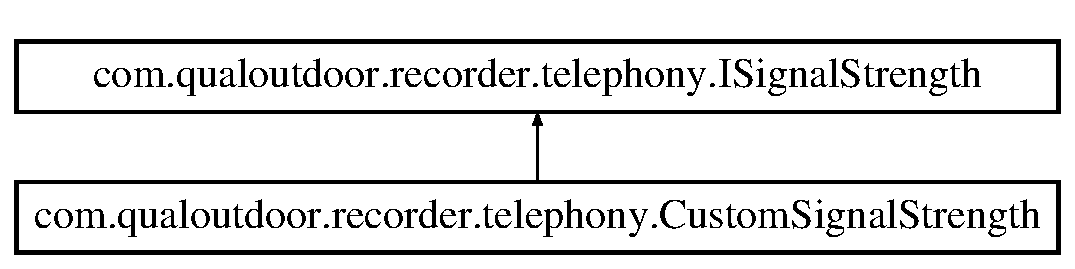
\includegraphics[height=2.000000cm]{classcom_1_1qualoutdoor_1_1recorder_1_1telephony_1_1CustomSignalStrength}
\end{center}
\end{figure}
\subsection*{Public Member Functions}
\begin{DoxyCompactItemize}
\item 
\hyperlink{classcom_1_1qualoutdoor_1_1recorder_1_1telephony_1_1CustomSignalStrength_aef90e4b781dd2f33444bf109b700a618}{Custom\-Signal\-Strength} (Signal\-Strength \hyperlink{classcom_1_1qualoutdoor_1_1recorder_1_1telephony_1_1CustomSignalStrength_aa3981bd9454f9a027a9b2f6697da62e3}{ss})
\item 
void \hyperlink{classcom_1_1qualoutdoor_1_1recorder_1_1telephony_1_1CustomSignalStrength_aef4df56064e24b3442dcb80ec1099b06}{set\-Signal\-Strength} (Signal\-Strength \hyperlink{classcom_1_1qualoutdoor_1_1recorder_1_1telephony_1_1CustomSignalStrength_aa3981bd9454f9a027a9b2f6697da62e3}{ss})
\item 
int \hyperlink{classcom_1_1qualoutdoor_1_1recorder_1_1telephony_1_1CustomSignalStrength_ad36ba58128637b99f41756dfccfe508f}{get\-Dbm} ()
\end{DoxyCompactItemize}
\subsection*{Private Attributes}
\begin{DoxyCompactItemize}
\item 
Signal\-Strength \hyperlink{classcom_1_1qualoutdoor_1_1recorder_1_1telephony_1_1CustomSignalStrength_aa3981bd9454f9a027a9b2f6697da62e3}{ss}
\end{DoxyCompactItemize}


\subsection{Detailed Description}


Definition at line 5 of file Custom\-Signal\-Strength.\-java.



\subsection{Constructor \& Destructor Documentation}
\hypertarget{classcom_1_1qualoutdoor_1_1recorder_1_1telephony_1_1CustomSignalStrength_aef90e4b781dd2f33444bf109b700a618}{\index{com\-::qualoutdoor\-::recorder\-::telephony\-::\-Custom\-Signal\-Strength@{com\-::qualoutdoor\-::recorder\-::telephony\-::\-Custom\-Signal\-Strength}!Custom\-Signal\-Strength@{Custom\-Signal\-Strength}}
\index{Custom\-Signal\-Strength@{Custom\-Signal\-Strength}!com::qualoutdoor::recorder::telephony::CustomSignalStrength@{com\-::qualoutdoor\-::recorder\-::telephony\-::\-Custom\-Signal\-Strength}}
\subsubsection[{Custom\-Signal\-Strength}]{\setlength{\rightskip}{0pt plus 5cm}com.\-qualoutdoor.\-recorder.\-telephony.\-Custom\-Signal\-Strength.\-Custom\-Signal\-Strength (
\begin{DoxyParamCaption}
\item[{Signal\-Strength}]{ss}
\end{DoxyParamCaption}
)}}\label{classcom_1_1qualoutdoor_1_1recorder_1_1telephony_1_1CustomSignalStrength_aef90e4b781dd2f33444bf109b700a618}
We can create a \hyperlink{classcom_1_1qualoutdoor_1_1recorder_1_1telephony_1_1CustomSignalStrength}{Custom\-Signal\-Strength} from the Android Signal\-Strength class 

Definition at line 14 of file Custom\-Signal\-Strength.\-java.



References com.\-qualoutdoor.\-recorder.\-telephony.\-Custom\-Signal\-Strength.\-ss.



\subsection{Member Function Documentation}
\hypertarget{classcom_1_1qualoutdoor_1_1recorder_1_1telephony_1_1CustomSignalStrength_ad36ba58128637b99f41756dfccfe508f}{\index{com\-::qualoutdoor\-::recorder\-::telephony\-::\-Custom\-Signal\-Strength@{com\-::qualoutdoor\-::recorder\-::telephony\-::\-Custom\-Signal\-Strength}!get\-Dbm@{get\-Dbm}}
\index{get\-Dbm@{get\-Dbm}!com::qualoutdoor::recorder::telephony::CustomSignalStrength@{com\-::qualoutdoor\-::recorder\-::telephony\-::\-Custom\-Signal\-Strength}}
\subsubsection[{get\-Dbm}]{\setlength{\rightskip}{0pt plus 5cm}int com.\-qualoutdoor.\-recorder.\-telephony.\-Custom\-Signal\-Strength.\-get\-Dbm (
\begin{DoxyParamCaption}
{}
\end{DoxyParamCaption}
)}}\label{classcom_1_1qualoutdoor_1_1recorder_1_1telephony_1_1CustomSignalStrength_ad36ba58128637b99f41756dfccfe508f}
Get the signal strength in d\-Bm 

Implements \hyperlink{interfacecom_1_1qualoutdoor_1_1recorder_1_1telephony_1_1ISignalStrength_a7afc6c43cd03481de1a10ab7c2770fa1}{com.\-qualoutdoor.\-recorder.\-telephony.\-I\-Signal\-Strength}.



Definition at line 24 of file Custom\-Signal\-Strength.\-java.

\hypertarget{classcom_1_1qualoutdoor_1_1recorder_1_1telephony_1_1CustomSignalStrength_aef4df56064e24b3442dcb80ec1099b06}{\index{com\-::qualoutdoor\-::recorder\-::telephony\-::\-Custom\-Signal\-Strength@{com\-::qualoutdoor\-::recorder\-::telephony\-::\-Custom\-Signal\-Strength}!set\-Signal\-Strength@{set\-Signal\-Strength}}
\index{set\-Signal\-Strength@{set\-Signal\-Strength}!com::qualoutdoor::recorder::telephony::CustomSignalStrength@{com\-::qualoutdoor\-::recorder\-::telephony\-::\-Custom\-Signal\-Strength}}
\subsubsection[{set\-Signal\-Strength}]{\setlength{\rightskip}{0pt plus 5cm}void com.\-qualoutdoor.\-recorder.\-telephony.\-Custom\-Signal\-Strength.\-set\-Signal\-Strength (
\begin{DoxyParamCaption}
\item[{Signal\-Strength}]{ss}
\end{DoxyParamCaption}
)}}\label{classcom_1_1qualoutdoor_1_1recorder_1_1telephony_1_1CustomSignalStrength_aef4df56064e24b3442dcb80ec1099b06}
Modify the signal strength value 

Definition at line 19 of file Custom\-Signal\-Strength.\-java.



References com.\-qualoutdoor.\-recorder.\-telephony.\-Custom\-Signal\-Strength.\-ss.



\subsection{Member Data Documentation}
\hypertarget{classcom_1_1qualoutdoor_1_1recorder_1_1telephony_1_1CustomSignalStrength_aa3981bd9454f9a027a9b2f6697da62e3}{\index{com\-::qualoutdoor\-::recorder\-::telephony\-::\-Custom\-Signal\-Strength@{com\-::qualoutdoor\-::recorder\-::telephony\-::\-Custom\-Signal\-Strength}!ss@{ss}}
\index{ss@{ss}!com::qualoutdoor::recorder::telephony::CustomSignalStrength@{com\-::qualoutdoor\-::recorder\-::telephony\-::\-Custom\-Signal\-Strength}}
\subsubsection[{ss}]{\setlength{\rightskip}{0pt plus 5cm}Signal\-Strength com.\-qualoutdoor.\-recorder.\-telephony.\-Custom\-Signal\-Strength.\-ss\hspace{0.3cm}{\ttfamily [private]}}}\label{classcom_1_1qualoutdoor_1_1recorder_1_1telephony_1_1CustomSignalStrength_aa3981bd9454f9a027a9b2f6697da62e3}
We encapsulate an Android Signal\-Strength instance 

Definition at line 8 of file Custom\-Signal\-Strength.\-java.



Referenced by com.\-qualoutdoor.\-recorder.\-telephony.\-Custom\-Signal\-Strength.\-Custom\-Signal\-Strength(), and com.\-qualoutdoor.\-recorder.\-telephony.\-Custom\-Signal\-Strength.\-set\-Signal\-Strength().



The documentation for this class was generated from the following file\-:\begin{DoxyCompactItemize}
\item 
src/com/qualoutdoor/recorder/telephony/Custom\-Signal\-Strength.\-java\end{DoxyCompactItemize}

\hypertarget{classcom_1_1qualoutdoor_1_1recorder_1_1map_1_1DataMapFragment}{\section{com.\-qualoutdoor.\-recorder.\-map.\-Data\-Map\-Fragment Class Reference}
\label{classcom_1_1qualoutdoor_1_1recorder_1_1map_1_1DataMapFragment}\index{com.\-qualoutdoor.\-recorder.\-map.\-Data\-Map\-Fragment@{com.\-qualoutdoor.\-recorder.\-map.\-Data\-Map\-Fragment}}
}
Inheritance diagram for com.\-qualoutdoor.\-recorder.\-map.\-Data\-Map\-Fragment\-:\begin{figure}[H]
\begin{center}
\leavevmode
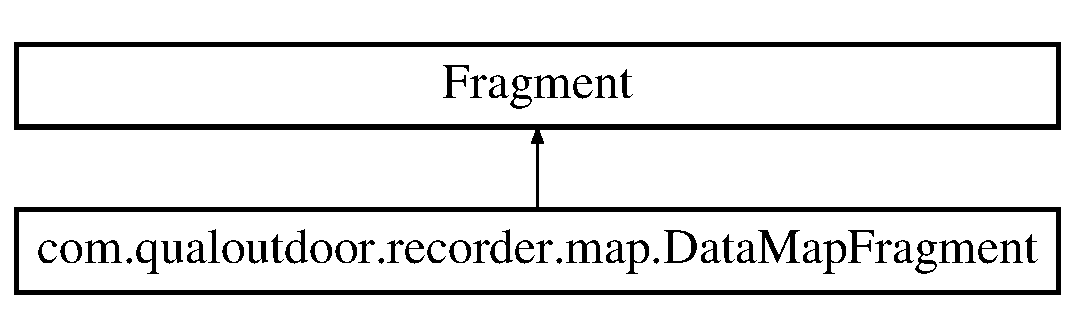
\includegraphics[height=2.000000cm]{classcom_1_1qualoutdoor_1_1recorder_1_1map_1_1DataMapFragment}
\end{center}
\end{figure}
\subsection*{Public Member Functions}
\begin{DoxyCompactItemize}
\item 
\hypertarget{classcom_1_1qualoutdoor_1_1recorder_1_1map_1_1DataMapFragment_a7b25f2611914b58fc774da31c4a22cbe}{void {\bfseries on\-Create} (Bundle saved\-Instance\-State)}\label{classcom_1_1qualoutdoor_1_1recorder_1_1map_1_1DataMapFragment_a7b25f2611914b58fc774da31c4a22cbe}

\item 
\hypertarget{classcom_1_1qualoutdoor_1_1recorder_1_1map_1_1DataMapFragment_a071cc429cc5e4bef51a728d3ca4dd1d6}{View {\bfseries on\-Create\-View} (Layout\-Inflater inflater, View\-Group container, Bundle saved\-Instance\-State)}\label{classcom_1_1qualoutdoor_1_1recorder_1_1map_1_1DataMapFragment_a071cc429cc5e4bef51a728d3ca4dd1d6}

\item 
\hypertarget{classcom_1_1qualoutdoor_1_1recorder_1_1map_1_1DataMapFragment_a8f9cf3ebd5f2943859294136dc013057}{void {\bfseries on\-Resume} ()}\label{classcom_1_1qualoutdoor_1_1recorder_1_1map_1_1DataMapFragment_a8f9cf3ebd5f2943859294136dc013057}

\end{DoxyCompactItemize}
\subsection*{Private Member Functions}
\begin{DoxyCompactItemize}
\item 
boolean \hyperlink{classcom_1_1qualoutdoor_1_1recorder_1_1map_1_1DataMapFragment_aec8e5d7ebd62ebda47d8bcb6469a45c4}{set\-Up\-Map\-If\-Needed} ()
\item 
void \hyperlink{classcom_1_1qualoutdoor_1_1recorder_1_1map_1_1DataMapFragment_ad61100353ce2562e4c09b00158e5a2ac}{init\-Markers} ()
\end{DoxyCompactItemize}
\subsection*{Private Attributes}
\begin{DoxyCompactItemize}
\item 
\hypertarget{classcom_1_1qualoutdoor_1_1recorder_1_1map_1_1DataMapFragment_a8818a618fb41bd86d8ba8735a87429c1}{Google\-Map {\bfseries map}}\label{classcom_1_1qualoutdoor_1_1recorder_1_1map_1_1DataMapFragment_a8818a618fb41bd86d8ba8735a87429c1}

\item 
\hypertarget{classcom_1_1qualoutdoor_1_1recorder_1_1map_1_1DataMapFragment_acd4640081a80fb7aff45ee8eacd41a26}{Support\-Map\-Fragment {\bfseries map\-Fragment}}\label{classcom_1_1qualoutdoor_1_1recorder_1_1map_1_1DataMapFragment_acd4640081a80fb7aff45ee8eacd41a26}

\end{DoxyCompactItemize}
\subsection*{Static Private Attributes}
\begin{DoxyCompactItemize}
\item 
\hypertarget{classcom_1_1qualoutdoor_1_1recorder_1_1map_1_1DataMapFragment_abf9b8e361549571285cf999f7eadf28c}{static int {\bfseries num\-Markers} = 25}\label{classcom_1_1qualoutdoor_1_1recorder_1_1map_1_1DataMapFragment_abf9b8e361549571285cf999f7eadf28c}

\item 
\hypertarget{classcom_1_1qualoutdoor_1_1recorder_1_1map_1_1DataMapFragment_a694479dfe8c0bb25d948eba8b8ef82d3}{static double {\bfseries melb\-Lat} = -\/37.\-813}\label{classcom_1_1qualoutdoor_1_1recorder_1_1map_1_1DataMapFragment_a694479dfe8c0bb25d948eba8b8ef82d3}

\item 
\hypertarget{classcom_1_1qualoutdoor_1_1recorder_1_1map_1_1DataMapFragment_afc47dba18d6c9b4b1cf8cf06a6b340ea}{static double {\bfseries melb\-Lng} = 144.\-962}\label{classcom_1_1qualoutdoor_1_1recorder_1_1map_1_1DataMapFragment_afc47dba18d6c9b4b1cf8cf06a6b340ea}

\item 
\hypertarget{classcom_1_1qualoutdoor_1_1recorder_1_1map_1_1DataMapFragment_a91e704a9e643164746f185e7b0d7cd20}{static Lat\-Lng {\bfseries melbournecenter} = new Lat\-Lng(melb\-Lat, melb\-Lng)}\label{classcom_1_1qualoutdoor_1_1recorder_1_1map_1_1DataMapFragment_a91e704a9e643164746f185e7b0d7cd20}

\item 
static Lat\-Lng {\bfseries southwest}
\item 
static Lat\-Lng {\bfseries northwest}
\item 
static Lat\-Lng\-Bounds {\bfseries melbourne}
\item 
\hypertarget{classcom_1_1qualoutdoor_1_1recorder_1_1map_1_1DataMapFragment_ae59f29056fb6c2660a0df13dd97f7104}{static double {\bfseries lat} = northwest.\-latitude -\/ southwest.\-latitude}\label{classcom_1_1qualoutdoor_1_1recorder_1_1map_1_1DataMapFragment_ae59f29056fb6c2660a0df13dd97f7104}

\item 
\hypertarget{classcom_1_1qualoutdoor_1_1recorder_1_1map_1_1DataMapFragment_a95712fa0c706d3d5b319708fe9f09e95}{static double {\bfseries lng} = northwest.\-longitude -\/ southwest.\-longitude}\label{classcom_1_1qualoutdoor_1_1recorder_1_1map_1_1DataMapFragment_a95712fa0c706d3d5b319708fe9f09e95}

\end{DoxyCompactItemize}


\subsection{Detailed Description}


Definition at line 27 of file Data\-Map\-Fragment.\-java.



\subsection{Member Function Documentation}
\hypertarget{classcom_1_1qualoutdoor_1_1recorder_1_1map_1_1DataMapFragment_ad61100353ce2562e4c09b00158e5a2ac}{\index{com\-::qualoutdoor\-::recorder\-::map\-::\-Data\-Map\-Fragment@{com\-::qualoutdoor\-::recorder\-::map\-::\-Data\-Map\-Fragment}!init\-Markers@{init\-Markers}}
\index{init\-Markers@{init\-Markers}!com::qualoutdoor::recorder::map::DataMapFragment@{com\-::qualoutdoor\-::recorder\-::map\-::\-Data\-Map\-Fragment}}
\subsubsection[{init\-Markers}]{\setlength{\rightskip}{0pt plus 5cm}void com.\-qualoutdoor.\-recorder.\-map.\-Data\-Map\-Fragment.\-init\-Markers (
\begin{DoxyParamCaption}
{}
\end{DoxyParamCaption}
)\hspace{0.3cm}{\ttfamily [private]}}}\label{classcom_1_1qualoutdoor_1_1recorder_1_1map_1_1DataMapFragment_ad61100353ce2562e4c09b00158e5a2ac}
Add the markers to the map 

Definition at line 131 of file Data\-Map\-Fragment.\-java.



Referenced by com.\-qualoutdoor.\-recorder.\-map.\-Data\-Map\-Fragment.\-set\-Up\-Map\-If\-Needed().

\hypertarget{classcom_1_1qualoutdoor_1_1recorder_1_1map_1_1DataMapFragment_aec8e5d7ebd62ebda47d8bcb6469a45c4}{\index{com\-::qualoutdoor\-::recorder\-::map\-::\-Data\-Map\-Fragment@{com\-::qualoutdoor\-::recorder\-::map\-::\-Data\-Map\-Fragment}!set\-Up\-Map\-If\-Needed@{set\-Up\-Map\-If\-Needed}}
\index{set\-Up\-Map\-If\-Needed@{set\-Up\-Map\-If\-Needed}!com::qualoutdoor::recorder::map::DataMapFragment@{com\-::qualoutdoor\-::recorder\-::map\-::\-Data\-Map\-Fragment}}
\subsubsection[{set\-Up\-Map\-If\-Needed}]{\setlength{\rightskip}{0pt plus 5cm}boolean com.\-qualoutdoor.\-recorder.\-map.\-Data\-Map\-Fragment.\-set\-Up\-Map\-If\-Needed (
\begin{DoxyParamCaption}
{}
\end{DoxyParamCaption}
)\hspace{0.3cm}{\ttfamily [private]}}}\label{classcom_1_1qualoutdoor_1_1recorder_1_1map_1_1DataMapFragment_aec8e5d7ebd62ebda47d8bcb6469a45c4}
Instantiate the Map object from the Map\-Fragment if needed. This is called from on\-Create and on\-Resume to ensure that the map is always available. Returns true if the map is available. 

Definition at line 106 of file Data\-Map\-Fragment.\-java.



References com.\-qualoutdoor.\-recorder.\-map.\-Data\-Map\-Fragment.\-init\-Markers().



\subsection{Member Data Documentation}
\hypertarget{classcom_1_1qualoutdoor_1_1recorder_1_1map_1_1DataMapFragment_aed652fd6268de6ddfe8bb36bb0a78762}{\index{com\-::qualoutdoor\-::recorder\-::map\-::\-Data\-Map\-Fragment@{com\-::qualoutdoor\-::recorder\-::map\-::\-Data\-Map\-Fragment}!melbourne@{melbourne}}
\index{melbourne@{melbourne}!com::qualoutdoor::recorder::map::DataMapFragment@{com\-::qualoutdoor\-::recorder\-::map\-::\-Data\-Map\-Fragment}}
\subsubsection[{melbourne}]{\setlength{\rightskip}{0pt plus 5cm}Lat\-Lng\-Bounds com.\-qualoutdoor.\-recorder.\-map.\-Data\-Map\-Fragment.\-melbourne\hspace{0.3cm}{\ttfamily [static]}, {\ttfamily [private]}}}\label{classcom_1_1qualoutdoor_1_1recorder_1_1map_1_1DataMapFragment_aed652fd6268de6ddfe8bb36bb0a78762}
{\bfseries Initial value\-:}
\begin{DoxyCode}
= \textcolor{keyword}{new} LatLngBounds(southwest,
            northwest)
\end{DoxyCode}


Definition at line 37 of file Data\-Map\-Fragment.\-java.

\hypertarget{classcom_1_1qualoutdoor_1_1recorder_1_1map_1_1DataMapFragment_a42c523ffb29115d4c52e3522412feb4a}{\index{com\-::qualoutdoor\-::recorder\-::map\-::\-Data\-Map\-Fragment@{com\-::qualoutdoor\-::recorder\-::map\-::\-Data\-Map\-Fragment}!northwest@{northwest}}
\index{northwest@{northwest}!com::qualoutdoor::recorder::map::DataMapFragment@{com\-::qualoutdoor\-::recorder\-::map\-::\-Data\-Map\-Fragment}}
\subsubsection[{northwest}]{\setlength{\rightskip}{0pt plus 5cm}Lat\-Lng com.\-qualoutdoor.\-recorder.\-map.\-Data\-Map\-Fragment.\-northwest\hspace{0.3cm}{\ttfamily [static]}, {\ttfamily [private]}}}\label{classcom_1_1qualoutdoor_1_1recorder_1_1map_1_1DataMapFragment_a42c523ffb29115d4c52e3522412feb4a}
{\bfseries Initial value\-:}
\begin{DoxyCode}
= \textcolor{keyword}{new} LatLng(melbLat + 0.015,
            melbLng + 0.015)
\end{DoxyCode}


Definition at line 35 of file Data\-Map\-Fragment.\-java.

\hypertarget{classcom_1_1qualoutdoor_1_1recorder_1_1map_1_1DataMapFragment_a3b6230c23fec1713a516ddafdde9a00d}{\index{com\-::qualoutdoor\-::recorder\-::map\-::\-Data\-Map\-Fragment@{com\-::qualoutdoor\-::recorder\-::map\-::\-Data\-Map\-Fragment}!southwest@{southwest}}
\index{southwest@{southwest}!com::qualoutdoor::recorder::map::DataMapFragment@{com\-::qualoutdoor\-::recorder\-::map\-::\-Data\-Map\-Fragment}}
\subsubsection[{southwest}]{\setlength{\rightskip}{0pt plus 5cm}Lat\-Lng com.\-qualoutdoor.\-recorder.\-map.\-Data\-Map\-Fragment.\-southwest\hspace{0.3cm}{\ttfamily [static]}, {\ttfamily [private]}}}\label{classcom_1_1qualoutdoor_1_1recorder_1_1map_1_1DataMapFragment_a3b6230c23fec1713a516ddafdde9a00d}
{\bfseries Initial value\-:}
\begin{DoxyCode}
= \textcolor{keyword}{new} LatLng(melbLat - 0.015,
            melbLng - 0.015)
\end{DoxyCode}


Definition at line 33 of file Data\-Map\-Fragment.\-java.



The documentation for this class was generated from the following file\-:\begin{DoxyCompactItemize}
\item 
src/com/qualoutdoor/recorder/map/Data\-Map\-Fragment.\-java\end{DoxyCompactItemize}

\hypertarget{classcom_1_1qualoutdoor_1_1recorder_1_1DisplayHelpActivity}{\section{com.\-qualoutdoor.\-recorder.\-Display\-Help\-Activity Class Reference}
\label{classcom_1_1qualoutdoor_1_1recorder_1_1DisplayHelpActivity}\index{com.\-qualoutdoor.\-recorder.\-Display\-Help\-Activity@{com.\-qualoutdoor.\-recorder.\-Display\-Help\-Activity}}
}
Inheritance diagram for com.\-qualoutdoor.\-recorder.\-Display\-Help\-Activity\-:\begin{figure}[H]
\begin{center}
\leavevmode
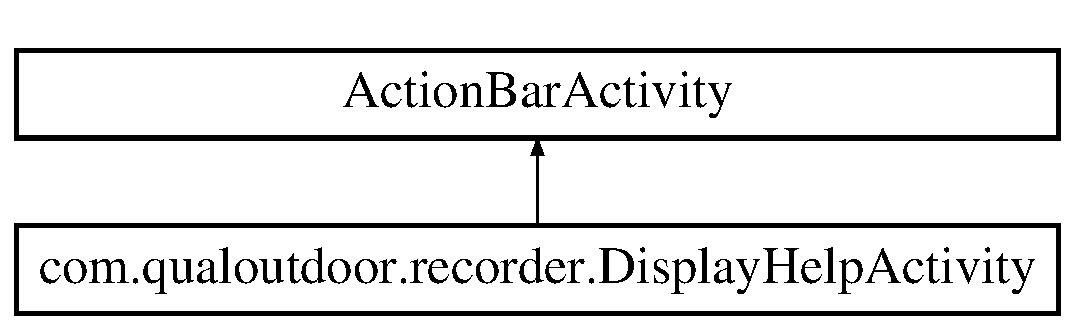
\includegraphics[height=2.000000cm]{classcom_1_1qualoutdoor_1_1recorder_1_1DisplayHelpActivity}
\end{center}
\end{figure}
\subsection*{Protected Member Functions}
\begin{DoxyCompactItemize}
\item 
\hypertarget{classcom_1_1qualoutdoor_1_1recorder_1_1DisplayHelpActivity_a69a3046becdab5fadc808588c4b28ad2}{void {\bfseries on\-Create} (Bundle saved\-Instance\-State)}\label{classcom_1_1qualoutdoor_1_1recorder_1_1DisplayHelpActivity_a69a3046becdab5fadc808588c4b28ad2}

\end{DoxyCompactItemize}


\subsection{Detailed Description}


Definition at line 6 of file Display\-Help\-Activity.\-java.



The documentation for this class was generated from the following file\-:\begin{DoxyCompactItemize}
\item 
src/com/qualoutdoor/recorder/Display\-Help\-Activity.\-java\end{DoxyCompactItemize}

\hypertarget{classcom_1_1qualoutdoor_1_1recorder_1_1settings_1_1DisplaySettingsFragment}{\section{com.\-qualoutdoor.\-recorder.\-settings.\-Display\-Settings\-Fragment Class Reference}
\label{classcom_1_1qualoutdoor_1_1recorder_1_1settings_1_1DisplaySettingsFragment}\index{com.\-qualoutdoor.\-recorder.\-settings.\-Display\-Settings\-Fragment@{com.\-qualoutdoor.\-recorder.\-settings.\-Display\-Settings\-Fragment}}
}
Inheritance diagram for com.\-qualoutdoor.\-recorder.\-settings.\-Display\-Settings\-Fragment\-:\begin{figure}[H]
\begin{center}
\leavevmode
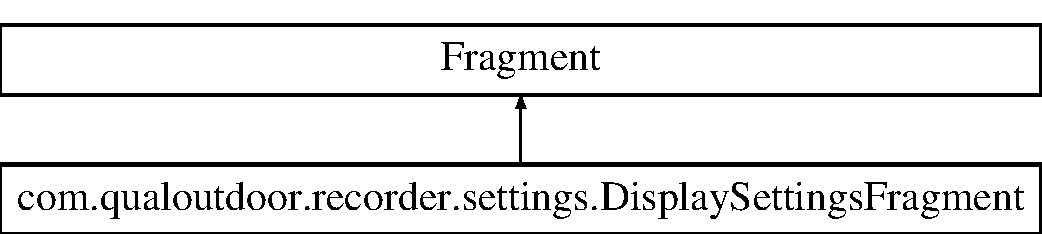
\includegraphics[height=2.000000cm]{classcom_1_1qualoutdoor_1_1recorder_1_1settings_1_1DisplaySettingsFragment}
\end{center}
\end{figure}
\subsection*{Public Member Functions}
\begin{DoxyCompactItemize}
\item 
\hypertarget{classcom_1_1qualoutdoor_1_1recorder_1_1settings_1_1DisplaySettingsFragment_aa4ba98386d247cdf2ff30da92bef8b39}{View {\bfseries on\-Create\-View} (Layout\-Inflater inflater, View\-Group container, Bundle saved\-Instance\-State)}\label{classcom_1_1qualoutdoor_1_1recorder_1_1settings_1_1DisplaySettingsFragment_aa4ba98386d247cdf2ff30da92bef8b39}

\end{DoxyCompactItemize}


\subsection{Detailed Description}
This fragment give access to the different settings sub-\/categories 

Definition at line 12 of file Display\-Settings\-Fragment.\-java.



The documentation for this class was generated from the following file\-:\begin{DoxyCompactItemize}
\item 
src/com/qualoutdoor/recorder/settings/Display\-Settings\-Fragment.\-java\end{DoxyCompactItemize}

\hypertarget{classcom_1_1qualoutdoor_1_1recorder_1_1MainActivity_1_1DrawerItemClickListener}{\section{com.\-qualoutdoor.\-recorder.\-Main\-Activity.\-Drawer\-Item\-Click\-Listener Class Reference}
\label{classcom_1_1qualoutdoor_1_1recorder_1_1MainActivity_1_1DrawerItemClickListener}\index{com.\-qualoutdoor.\-recorder.\-Main\-Activity.\-Drawer\-Item\-Click\-Listener@{com.\-qualoutdoor.\-recorder.\-Main\-Activity.\-Drawer\-Item\-Click\-Listener}}
}
Inheritance diagram for com.\-qualoutdoor.\-recorder.\-Main\-Activity.\-Drawer\-Item\-Click\-Listener\-:\begin{figure}[H]
\begin{center}
\leavevmode
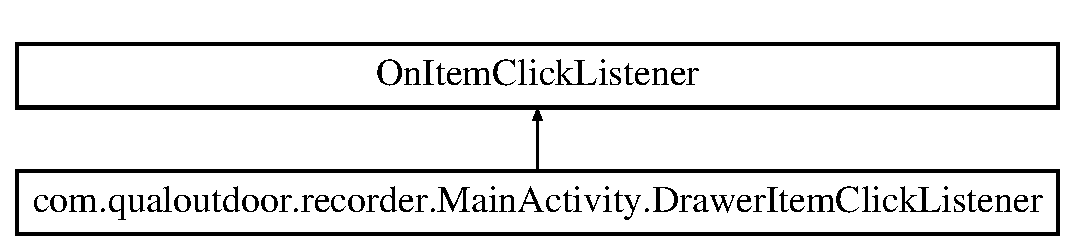
\includegraphics[height=2.000000cm]{classcom_1_1qualoutdoor_1_1recorder_1_1MainActivity_1_1DrawerItemClickListener}
\end{center}
\end{figure}
\subsection*{Public Member Functions}
\begin{DoxyCompactItemize}
\item 
\hypertarget{classcom_1_1qualoutdoor_1_1recorder_1_1MainActivity_1_1DrawerItemClickListener_af8d7abb968131246e1ebafdacde9a9b4}{void {\bfseries on\-Item\-Click} (Adapter\-View$<$?$>$ parent, View view, int position, long id)}\label{classcom_1_1qualoutdoor_1_1recorder_1_1MainActivity_1_1DrawerItemClickListener_af8d7abb968131246e1ebafdacde9a9b4}

\end{DoxyCompactItemize}


\subsection{Detailed Description}
The navigation drawer items click listener 

Definition at line 248 of file Main\-Activity.\-java.



The documentation for this class was generated from the following file\-:\begin{DoxyCompactItemize}
\item 
src/com/qualoutdoor/recorder/Main\-Activity.\-java\end{DoxyCompactItemize}

\hypertarget{classcom_1_1qualoutdoor_1_1recorder_1_1GenericFragment}{\section{com.\-qualoutdoor.\-recorder.\-Generic\-Fragment Class Reference}
\label{classcom_1_1qualoutdoor_1_1recorder_1_1GenericFragment}\index{com.\-qualoutdoor.\-recorder.\-Generic\-Fragment@{com.\-qualoutdoor.\-recorder.\-Generic\-Fragment}}
}
Inheritance diagram for com.\-qualoutdoor.\-recorder.\-Generic\-Fragment\-:\begin{figure}[H]
\begin{center}
\leavevmode
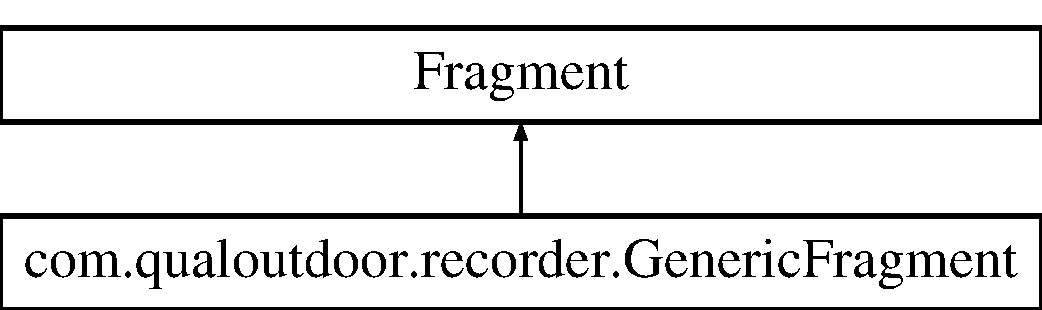
\includegraphics[height=2.000000cm]{classcom_1_1qualoutdoor_1_1recorder_1_1GenericFragment}
\end{center}
\end{figure}
\subsection*{Public Member Functions}
\begin{DoxyCompactItemize}
\item 
\hypertarget{classcom_1_1qualoutdoor_1_1recorder_1_1GenericFragment_a6e5febce9c3aee57b19b8f0aa25229cd}{void {\bfseries on\-Create} (Bundle saved\-Instance\-State)}\label{classcom_1_1qualoutdoor_1_1recorder_1_1GenericFragment_a6e5febce9c3aee57b19b8f0aa25229cd}

\item 
\hypertarget{classcom_1_1qualoutdoor_1_1recorder_1_1GenericFragment_a0d7034fbb93cf8bfdb55fe5668f63896}{View {\bfseries on\-Create\-View} (Layout\-Inflater inflater, View\-Group container, Bundle saved\-Instance\-State)}\label{classcom_1_1qualoutdoor_1_1recorder_1_1GenericFragment_a0d7034fbb93cf8bfdb55fe5668f63896}

\end{DoxyCompactItemize}
\subsection*{Static Public Attributes}
\begin{DoxyCompactItemize}
\item 
\hypertarget{classcom_1_1qualoutdoor_1_1recorder_1_1GenericFragment_a49ec6e272a29d2f83d75597ad4820186}{static final String {\bfseries F\-R\-A\-G\-M\-E\-N\-T\-\_\-\-N\-A\-M\-E} = \char`\"{}fragment\-\_\-name\char`\"{}}\label{classcom_1_1qualoutdoor_1_1recorder_1_1GenericFragment_a49ec6e272a29d2f83d75597ad4820186}

\end{DoxyCompactItemize}
\subsection*{Private Attributes}
\begin{DoxyCompactItemize}
\item 
Char\-Sequence \hyperlink{classcom_1_1qualoutdoor_1_1recorder_1_1GenericFragment_abd35750acf1a4b68e302201fc4cc3132}{name} = \char`\"{}Generic Fragment\char`\"{}
\end{DoxyCompactItemize}


\subsection{Detailed Description}
A generic fragment, to be used in place of a 'non implemented yet fragment'. 

Definition at line 11 of file Generic\-Fragment.\-java.



\subsection{Member Data Documentation}
\hypertarget{classcom_1_1qualoutdoor_1_1recorder_1_1GenericFragment_abd35750acf1a4b68e302201fc4cc3132}{\index{com\-::qualoutdoor\-::recorder\-::\-Generic\-Fragment@{com\-::qualoutdoor\-::recorder\-::\-Generic\-Fragment}!name@{name}}
\index{name@{name}!com::qualoutdoor::recorder::GenericFragment@{com\-::qualoutdoor\-::recorder\-::\-Generic\-Fragment}}
\subsubsection[{name}]{\setlength{\rightskip}{0pt plus 5cm}Char\-Sequence com.\-qualoutdoor.\-recorder.\-Generic\-Fragment.\-name = \char`\"{}Generic Fragment\char`\"{}\hspace{0.3cm}{\ttfamily [private]}}}\label{classcom_1_1qualoutdoor_1_1recorder_1_1GenericFragment_abd35750acf1a4b68e302201fc4cc3132}
The name of the generic fragment (and the name to display) 

Definition at line 17 of file Generic\-Fragment.\-java.



The documentation for this class was generated from the following file\-:\begin{DoxyCompactItemize}
\item 
src/com/qualoutdoor/recorder/Generic\-Fragment.\-java\end{DoxyCompactItemize}

\hypertarget{interfacecom_1_1qualoutdoor_1_1recorder_1_1telephony_1_1ICellInfo}{\section{com.\-qualoutdoor.\-recorder.\-telephony.\-I\-Cell\-Info Interface Reference}
\label{interfacecom_1_1qualoutdoor_1_1recorder_1_1telephony_1_1ICellInfo}\index{com.\-qualoutdoor.\-recorder.\-telephony.\-I\-Cell\-Info@{com.\-qualoutdoor.\-recorder.\-telephony.\-I\-Cell\-Info}}
}
\subsection*{Public Member Functions}
\begin{DoxyCompactItemize}
\item 
long \hyperlink{interfacecom_1_1qualoutdoor_1_1recorder_1_1telephony_1_1ICellInfo_a20aaca32b7aad64bca27b703e4f6dbb5}{get\-Time\-Stamp} ()
\item 
boolean \hyperlink{interfacecom_1_1qualoutdoor_1_1recorder_1_1telephony_1_1ICellInfo_aced3d6782e7e962ab4a92e2e8af5e280}{is\-Registered} ()
\item 
void \hyperlink{interfacecom_1_1qualoutdoor_1_1recorder_1_1telephony_1_1ICellInfo_a99a2515d30d7a0b7c667e23690fb5d09}{todo} ()
\end{DoxyCompactItemize}


\subsection{Detailed Description}
This is an interface for accessing a cell information 

Definition at line 4 of file I\-Cell\-Info.\-java.



\subsection{Member Function Documentation}
\hypertarget{interfacecom_1_1qualoutdoor_1_1recorder_1_1telephony_1_1ICellInfo_a20aaca32b7aad64bca27b703e4f6dbb5}{\index{com\-::qualoutdoor\-::recorder\-::telephony\-::\-I\-Cell\-Info@{com\-::qualoutdoor\-::recorder\-::telephony\-::\-I\-Cell\-Info}!get\-Time\-Stamp@{get\-Time\-Stamp}}
\index{get\-Time\-Stamp@{get\-Time\-Stamp}!com::qualoutdoor::recorder::telephony::ICellInfo@{com\-::qualoutdoor\-::recorder\-::telephony\-::\-I\-Cell\-Info}}
\subsubsection[{get\-Time\-Stamp}]{\setlength{\rightskip}{0pt plus 5cm}long com.\-qualoutdoor.\-recorder.\-telephony.\-I\-Cell\-Info.\-get\-Time\-Stamp (
\begin{DoxyParamCaption}
{}
\end{DoxyParamCaption}
)}}\label{interfacecom_1_1qualoutdoor_1_1recorder_1_1telephony_1_1ICellInfo_a20aaca32b7aad64bca27b703e4f6dbb5}
Approximate time of this cell information in nanoseconds since boot \hypertarget{interfacecom_1_1qualoutdoor_1_1recorder_1_1telephony_1_1ICellInfo_aced3d6782e7e962ab4a92e2e8af5e280}{\index{com\-::qualoutdoor\-::recorder\-::telephony\-::\-I\-Cell\-Info@{com\-::qualoutdoor\-::recorder\-::telephony\-::\-I\-Cell\-Info}!is\-Registered@{is\-Registered}}
\index{is\-Registered@{is\-Registered}!com::qualoutdoor::recorder::telephony::ICellInfo@{com\-::qualoutdoor\-::recorder\-::telephony\-::\-I\-Cell\-Info}}
\subsubsection[{is\-Registered}]{\setlength{\rightskip}{0pt plus 5cm}boolean com.\-qualoutdoor.\-recorder.\-telephony.\-I\-Cell\-Info.\-is\-Registered (
\begin{DoxyParamCaption}
{}
\end{DoxyParamCaption}
)}}\label{interfacecom_1_1qualoutdoor_1_1recorder_1_1telephony_1_1ICellInfo_aced3d6782e7e962ab4a92e2e8af5e280}
True if this cell is registered to the network \hypertarget{interfacecom_1_1qualoutdoor_1_1recorder_1_1telephony_1_1ICellInfo_a99a2515d30d7a0b7c667e23690fb5d09}{\index{com\-::qualoutdoor\-::recorder\-::telephony\-::\-I\-Cell\-Info@{com\-::qualoutdoor\-::recorder\-::telephony\-::\-I\-Cell\-Info}!todo@{todo}}
\index{todo@{todo}!com::qualoutdoor::recorder::telephony::ICellInfo@{com\-::qualoutdoor\-::recorder\-::telephony\-::\-I\-Cell\-Info}}
\subsubsection[{todo}]{\setlength{\rightskip}{0pt plus 5cm}void com.\-qualoutdoor.\-recorder.\-telephony.\-I\-Cell\-Info.\-todo (
\begin{DoxyParamCaption}
{}
\end{DoxyParamCaption}
)}}\label{interfacecom_1_1qualoutdoor_1_1recorder_1_1telephony_1_1ICellInfo_a99a2515d30d7a0b7c667e23690fb5d09}
Others methods need to be added 

The documentation for this interface was generated from the following file\-:\begin{DoxyCompactItemize}
\item 
src/com/qualoutdoor/recorder/telephony/I\-Cell\-Info.\-java\end{DoxyCompactItemize}

\hypertarget{interfacecom_1_1qualoutdoor_1_1recorder_1_1telephony_1_1ILocation}{\section{com.\-qualoutdoor.\-recorder.\-telephony.\-I\-Location Interface Reference}
\label{interfacecom_1_1qualoutdoor_1_1recorder_1_1telephony_1_1ILocation}\index{com.\-qualoutdoor.\-recorder.\-telephony.\-I\-Location@{com.\-qualoutdoor.\-recorder.\-telephony.\-I\-Location}}
}
\subsection*{Public Member Functions}
\begin{DoxyCompactItemize}
\item 
long \hyperlink{interfacecom_1_1qualoutdoor_1_1recorder_1_1telephony_1_1ILocation_ab5830a326501790c9a62299aa87a8647}{get\-Time} ()
\item 
double \hyperlink{interfacecom_1_1qualoutdoor_1_1recorder_1_1telephony_1_1ILocation_a931dbc3d8450e9eb5b2dbca4353f2f33}{get\-Altitude} ()
\item 
double \hyperlink{interfacecom_1_1qualoutdoor_1_1recorder_1_1telephony_1_1ILocation_aa96b362e0fae13e0ee765d2ec68f11c5}{get\-Longitude} ()
\item 
float \hyperlink{interfacecom_1_1qualoutdoor_1_1recorder_1_1telephony_1_1ILocation_a9f7cc64e71a367c097b4bf247525c670}{get\-Accuracy} ()
\end{DoxyCompactItemize}


\subsection{Detailed Description}
This is an interface for accessing a location details 

Definition at line 4 of file I\-Location.\-java.



\subsection{Member Function Documentation}
\hypertarget{interfacecom_1_1qualoutdoor_1_1recorder_1_1telephony_1_1ILocation_a9f7cc64e71a367c097b4bf247525c670}{\index{com\-::qualoutdoor\-::recorder\-::telephony\-::\-I\-Location@{com\-::qualoutdoor\-::recorder\-::telephony\-::\-I\-Location}!get\-Accuracy@{get\-Accuracy}}
\index{get\-Accuracy@{get\-Accuracy}!com::qualoutdoor::recorder::telephony::ILocation@{com\-::qualoutdoor\-::recorder\-::telephony\-::\-I\-Location}}
\subsubsection[{get\-Accuracy}]{\setlength{\rightskip}{0pt plus 5cm}float com.\-qualoutdoor.\-recorder.\-telephony.\-I\-Location.\-get\-Accuracy (
\begin{DoxyParamCaption}
{}
\end{DoxyParamCaption}
)}}\label{interfacecom_1_1qualoutdoor_1_1recorder_1_1telephony_1_1ILocation_a9f7cc64e71a367c097b4bf247525c670}
Get the estimated accuracy of this location, in meters \hypertarget{interfacecom_1_1qualoutdoor_1_1recorder_1_1telephony_1_1ILocation_a931dbc3d8450e9eb5b2dbca4353f2f33}{\index{com\-::qualoutdoor\-::recorder\-::telephony\-::\-I\-Location@{com\-::qualoutdoor\-::recorder\-::telephony\-::\-I\-Location}!get\-Altitude@{get\-Altitude}}
\index{get\-Altitude@{get\-Altitude}!com::qualoutdoor::recorder::telephony::ILocation@{com\-::qualoutdoor\-::recorder\-::telephony\-::\-I\-Location}}
\subsubsection[{get\-Altitude}]{\setlength{\rightskip}{0pt plus 5cm}double com.\-qualoutdoor.\-recorder.\-telephony.\-I\-Location.\-get\-Altitude (
\begin{DoxyParamCaption}
{}
\end{DoxyParamCaption}
)}}\label{interfacecom_1_1qualoutdoor_1_1recorder_1_1telephony_1_1ILocation_a931dbc3d8450e9eb5b2dbca4353f2f33}
Get the latitude, in degrees \hypertarget{interfacecom_1_1qualoutdoor_1_1recorder_1_1telephony_1_1ILocation_aa96b362e0fae13e0ee765d2ec68f11c5}{\index{com\-::qualoutdoor\-::recorder\-::telephony\-::\-I\-Location@{com\-::qualoutdoor\-::recorder\-::telephony\-::\-I\-Location}!get\-Longitude@{get\-Longitude}}
\index{get\-Longitude@{get\-Longitude}!com::qualoutdoor::recorder::telephony::ILocation@{com\-::qualoutdoor\-::recorder\-::telephony\-::\-I\-Location}}
\subsubsection[{get\-Longitude}]{\setlength{\rightskip}{0pt plus 5cm}double com.\-qualoutdoor.\-recorder.\-telephony.\-I\-Location.\-get\-Longitude (
\begin{DoxyParamCaption}
{}
\end{DoxyParamCaption}
)}}\label{interfacecom_1_1qualoutdoor_1_1recorder_1_1telephony_1_1ILocation_aa96b362e0fae13e0ee765d2ec68f11c5}
Get the longitude, in degrees \hypertarget{interfacecom_1_1qualoutdoor_1_1recorder_1_1telephony_1_1ILocation_ab5830a326501790c9a62299aa87a8647}{\index{com\-::qualoutdoor\-::recorder\-::telephony\-::\-I\-Location@{com\-::qualoutdoor\-::recorder\-::telephony\-::\-I\-Location}!get\-Time@{get\-Time}}
\index{get\-Time@{get\-Time}!com::qualoutdoor::recorder::telephony::ILocation@{com\-::qualoutdoor\-::recorder\-::telephony\-::\-I\-Location}}
\subsubsection[{get\-Time}]{\setlength{\rightskip}{0pt plus 5cm}long com.\-qualoutdoor.\-recorder.\-telephony.\-I\-Location.\-get\-Time (
\begin{DoxyParamCaption}
{}
\end{DoxyParamCaption}
)}}\label{interfacecom_1_1qualoutdoor_1_1recorder_1_1telephony_1_1ILocation_ab5830a326501790c9a62299aa87a8647}
Return the U\-T\-C time of this data, in milliseconds since January 1, 1970 

The documentation for this interface was generated from the following file\-:\begin{DoxyCompactItemize}
\item 
src/com/qualoutdoor/recorder/telephony/I\-Location.\-java\end{DoxyCompactItemize}

\hypertarget{interfacecom_1_1qualoutdoor_1_1recorder_1_1telephony_1_1ISignalStrength}{\section{com.\-qualoutdoor.\-recorder.\-telephony.\-I\-Signal\-Strength Interface Reference}
\label{interfacecom_1_1qualoutdoor_1_1recorder_1_1telephony_1_1ISignalStrength}\index{com.\-qualoutdoor.\-recorder.\-telephony.\-I\-Signal\-Strength@{com.\-qualoutdoor.\-recorder.\-telephony.\-I\-Signal\-Strength}}
}
Inheritance diagram for com.\-qualoutdoor.\-recorder.\-telephony.\-I\-Signal\-Strength\-:\begin{figure}[H]
\begin{center}
\leavevmode
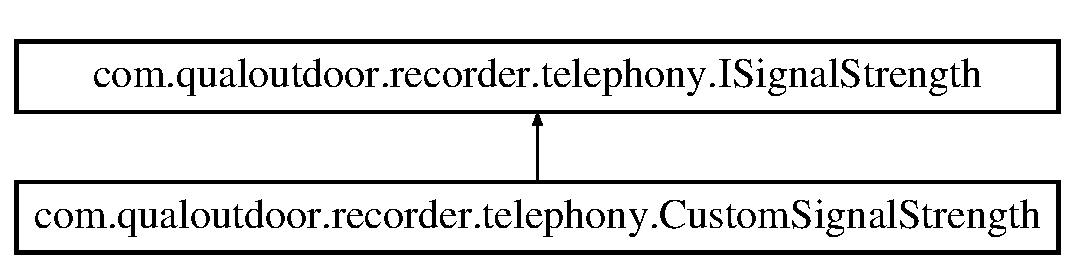
\includegraphics[height=2.000000cm]{interfacecom_1_1qualoutdoor_1_1recorder_1_1telephony_1_1ISignalStrength}
\end{center}
\end{figure}
\subsection*{Public Member Functions}
\begin{DoxyCompactItemize}
\item 
int \hyperlink{interfacecom_1_1qualoutdoor_1_1recorder_1_1telephony_1_1ISignalStrength_a7afc6c43cd03481de1a10ab7c2770fa1}{get\-Dbm} ()
\end{DoxyCompactItemize}


\subsection{Detailed Description}
This is an interface for accessing a signal strength information 

Definition at line 4 of file I\-Signal\-Strength.\-java.



\subsection{Member Function Documentation}
\hypertarget{interfacecom_1_1qualoutdoor_1_1recorder_1_1telephony_1_1ISignalStrength_a7afc6c43cd03481de1a10ab7c2770fa1}{\index{com\-::qualoutdoor\-::recorder\-::telephony\-::\-I\-Signal\-Strength@{com\-::qualoutdoor\-::recorder\-::telephony\-::\-I\-Signal\-Strength}!get\-Dbm@{get\-Dbm}}
\index{get\-Dbm@{get\-Dbm}!com::qualoutdoor::recorder::telephony::ISignalStrength@{com\-::qualoutdoor\-::recorder\-::telephony\-::\-I\-Signal\-Strength}}
\subsubsection[{get\-Dbm}]{\setlength{\rightskip}{0pt plus 5cm}int com.\-qualoutdoor.\-recorder.\-telephony.\-I\-Signal\-Strength.\-get\-Dbm (
\begin{DoxyParamCaption}
{}
\end{DoxyParamCaption}
)}}\label{interfacecom_1_1qualoutdoor_1_1recorder_1_1telephony_1_1ISignalStrength_a7afc6c43cd03481de1a10ab7c2770fa1}
Get the signal strength in d\-Bm 

Implemented in \hyperlink{classcom_1_1qualoutdoor_1_1recorder_1_1telephony_1_1CustomSignalStrength_ad36ba58128637b99f41756dfccfe508f}{com.\-qualoutdoor.\-recorder.\-telephony.\-Custom\-Signal\-Strength}.



The documentation for this interface was generated from the following file\-:\begin{DoxyCompactItemize}
\item 
src/com/qualoutdoor/recorder/telephony/I\-Signal\-Strength.\-java\end{DoxyCompactItemize}

\hypertarget{interfacecom_1_1qualoutdoor_1_1recorder_1_1telephony_1_1ITelephony}{\section{com.\-qualoutdoor.\-recorder.\-telephony.\-I\-Telephony Interface Reference}
\label{interfacecom_1_1qualoutdoor_1_1recorder_1_1telephony_1_1ITelephony}\index{com.\-qualoutdoor.\-recorder.\-telephony.\-I\-Telephony@{com.\-qualoutdoor.\-recorder.\-telephony.\-I\-Telephony}}
}
Inheritance diagram for com.\-qualoutdoor.\-recorder.\-telephony.\-I\-Telephony\-:\begin{figure}[H]
\begin{center}
\leavevmode
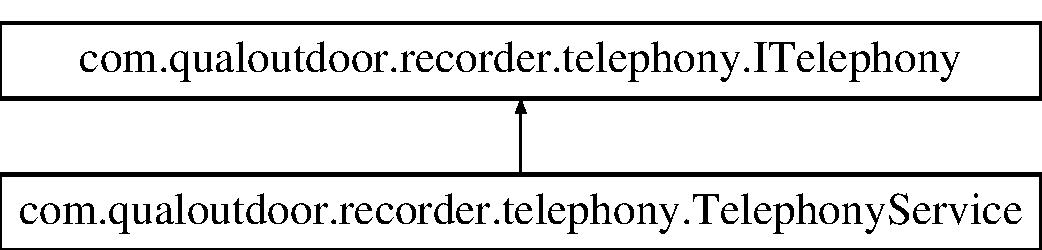
\includegraphics[height=2.000000cm]{interfacecom_1_1qualoutdoor_1_1recorder_1_1telephony_1_1ITelephony}
\end{center}
\end{figure}
\subsection*{Public Member Functions}
\begin{DoxyCompactItemize}
\item 
List$<$ \hyperlink{interfacecom_1_1qualoutdoor_1_1recorder_1_1telephony_1_1ICellInfo}{I\-Cell\-Info} $>$ \hyperlink{interfacecom_1_1qualoutdoor_1_1recorder_1_1telephony_1_1ITelephony_ac5f0965e1dfccd7207f49c277593acaa}{get\-All\-Cell\-Info} ()
\item 
int \hyperlink{interfacecom_1_1qualoutdoor_1_1recorder_1_1telephony_1_1ITelephony_a1b955c3be64a899274bf112d05c8d41a}{get\-Call\-State} ()
\item 
int \hyperlink{interfacecom_1_1qualoutdoor_1_1recorder_1_1telephony_1_1ITelephony_ab4135b0c4f01f0169b3a1ea63054b946}{get\-Data\-State} ()
\item 
int \hyperlink{interfacecom_1_1qualoutdoor_1_1recorder_1_1telephony_1_1ITelephony_af19331bac8e7317958047a5448274a28}{get\-Network\-Type} ()
\item 
\hyperlink{interfacecom_1_1qualoutdoor_1_1recorder_1_1telephony_1_1ILocation}{I\-Location} \hyperlink{interfacecom_1_1qualoutdoor_1_1recorder_1_1telephony_1_1ITelephony_acb95b0c4243cfca3c56776fc0ae3d18e}{get\-Location} ()
\item 
\hyperlink{interfacecom_1_1qualoutdoor_1_1recorder_1_1telephony_1_1ISignalStrength}{I\-Signal\-Strength} \hyperlink{interfacecom_1_1qualoutdoor_1_1recorder_1_1telephony_1_1ITelephony_a3454755b99a36692f8ed113144491760}{get\-Signal\-Strength} ()
\item 
void \hyperlink{interfacecom_1_1qualoutdoor_1_1recorder_1_1telephony_1_1ITelephony_a2bf33ee65f59c2100442f6ba33fac113}{listen} (\hyperlink{classcom_1_1qualoutdoor_1_1recorder_1_1telephony_1_1TelephonyListener}{Telephony\-Listener} listener, int events)
\item 
void \hyperlink{interfacecom_1_1qualoutdoor_1_1recorder_1_1telephony_1_1ITelephony_aaa52e62dfb4607e2f871e3ad0daeba23}{set\-Minimum\-Refresh\-Rate} (int milliseconds)
\end{DoxyCompactItemize}
\subsection*{Static Public Attributes}
\begin{DoxyCompactItemize}
\item 
static final int \hyperlink{interfacecom_1_1qualoutdoor_1_1recorder_1_1telephony_1_1ITelephony_ab2d6e4c2dd160412dda46b26763e8a64}{C\-A\-L\-L\-\_\-\-S\-T\-A\-T\-E\-\_\-\-I\-D\-L\-E} = 0
\item 
static final int \hyperlink{interfacecom_1_1qualoutdoor_1_1recorder_1_1telephony_1_1ITelephony_a2efb64f0209a5ae97c7cb331827c80a9}{C\-A\-L\-L\-\_\-\-S\-T\-A\-T\-E\-\_\-\-O\-F\-F\-H\-O\-O\-K} = 2
\item 
static final int \hyperlink{interfacecom_1_1qualoutdoor_1_1recorder_1_1telephony_1_1ITelephony_aea753bfaf3bdcab76c67409284bd3aab}{C\-A\-L\-L\-\_\-\-S\-T\-A\-T\-E\-\_\-\-R\-I\-N\-G\-I\-N\-G} = 1
\item 
static final int \hyperlink{interfacecom_1_1qualoutdoor_1_1recorder_1_1telephony_1_1ITelephony_a1d4417783954f4f1a82ade95bf2617b3}{D\-A\-T\-A\-\_\-\-C\-O\-N\-N\-E\-C\-T\-E\-D} = 2
\item 
static final int \hyperlink{interfacecom_1_1qualoutdoor_1_1recorder_1_1telephony_1_1ITelephony_a0fed369a5e327ef1100f8bb86ba8283e}{D\-A\-T\-A\-\_\-\-C\-O\-N\-N\-E\-C\-T\-I\-N\-G} = 1
\item 
static final int \hyperlink{interfacecom_1_1qualoutdoor_1_1recorder_1_1telephony_1_1ITelephony_a918bc00a6b832ab07926cf77626bbd24}{D\-A\-T\-A\-\_\-\-D\-I\-S\-C\-O\-N\-N\-E\-C\-T\-E\-D} = 0
\item 
static final int \hyperlink{interfacecom_1_1qualoutdoor_1_1recorder_1_1telephony_1_1ITelephony_adbd921850a2b4a6558f41dea27e861e0}{D\-A\-T\-A\-\_\-\-S\-U\-S\-P\-E\-N\-D\-E\-D} = 3
\item 
static final int \hyperlink{interfacecom_1_1qualoutdoor_1_1recorder_1_1telephony_1_1ITelephony_a673927b5b9f59f4adfdbbe8403dc3f75}{N\-E\-T\-W\-O\-R\-K\-\_\-\-T\-Y\-P\-E\-\_\-\-U\-N\-K\-N\-O\-W\-N} = 0
\item 
static final int \hyperlink{interfacecom_1_1qualoutdoor_1_1recorder_1_1telephony_1_1ITelephony_a370a400527daeffcf74e59bb8c25783f}{N\-E\-T\-W\-O\-R\-K\-\_\-\-T\-Y\-P\-E\-\_\-\-G\-P\-R\-S} = 1
\item 
static final int \hyperlink{interfacecom_1_1qualoutdoor_1_1recorder_1_1telephony_1_1ITelephony_a24b6cda1c698dedf417e58b3742acf02}{N\-E\-T\-W\-O\-R\-K\-\_\-\-T\-Y\-P\-E\-\_\-\-E\-D\-G\-E} = 2
\item 
static final int \hyperlink{interfacecom_1_1qualoutdoor_1_1recorder_1_1telephony_1_1ITelephony_a8135b29f493e56a852c6938f094e370c}{N\-E\-T\-W\-O\-R\-K\-\_\-\-T\-Y\-P\-E\-\_\-\-U\-M\-T\-S} = 3
\item 
static final int \hyperlink{interfacecom_1_1qualoutdoor_1_1recorder_1_1telephony_1_1ITelephony_a8242847ab2e7f8cd3b9a4ca0af7789aa}{N\-E\-T\-W\-O\-R\-K\-\_\-\-T\-Y\-P\-E\-\_\-\-C\-D\-M\-A} = 4
\item 
static final int \hyperlink{interfacecom_1_1qualoutdoor_1_1recorder_1_1telephony_1_1ITelephony_a17d25ab25bf982026aa45b3f4d29ceb5}{N\-E\-T\-W\-O\-R\-K\-\_\-\-T\-Y\-P\-E\-\_\-\-E\-V\-D\-O\-\_\-0} = 5
\item 
static final int \hyperlink{interfacecom_1_1qualoutdoor_1_1recorder_1_1telephony_1_1ITelephony_a9ea0965450da41c68810e4e071b2230e}{N\-E\-T\-W\-O\-R\-K\-\_\-\-T\-Y\-P\-E\-\_\-\-E\-V\-D\-O\-\_\-\-A} = 6
\item 
static final int \hyperlink{interfacecom_1_1qualoutdoor_1_1recorder_1_1telephony_1_1ITelephony_a4203966c4736f3023fc7940671f058d0}{N\-E\-T\-W\-O\-R\-K\-\_\-\-T\-Y\-P\-E\-\_\-1x\-R\-T\-T} = 7
\item 
static final int \hyperlink{interfacecom_1_1qualoutdoor_1_1recorder_1_1telephony_1_1ITelephony_af03c317a10fcccd01008912fa27b8f25}{N\-E\-T\-W\-O\-R\-K\-\_\-\-T\-Y\-P\-E\-\_\-\-H\-S\-D\-P\-A} = 8
\item 
static final int \hyperlink{interfacecom_1_1qualoutdoor_1_1recorder_1_1telephony_1_1ITelephony_a8508ef692db2bba21961b1e213b3440d}{N\-E\-T\-W\-O\-R\-K\-\_\-\-T\-Y\-P\-E\-\_\-\-H\-S\-U\-P\-A} = 9
\item 
static final int \hyperlink{interfacecom_1_1qualoutdoor_1_1recorder_1_1telephony_1_1ITelephony_a90ea3934af7570fac6e9c4787b130d2a}{N\-E\-T\-W\-O\-R\-K\-\_\-\-T\-Y\-P\-E\-\_\-\-H\-S\-P\-A} = 10
\item 
static final int \hyperlink{interfacecom_1_1qualoutdoor_1_1recorder_1_1telephony_1_1ITelephony_ad7af57643bf08eb193e93557d4c40e53}{N\-E\-T\-W\-O\-R\-K\-\_\-\-T\-Y\-P\-E\-\_\-\-I\-D\-E\-N} = 11
\item 
static final int \hyperlink{interfacecom_1_1qualoutdoor_1_1recorder_1_1telephony_1_1ITelephony_a9c5eee3774b26ae94b26fa7a41dfe75e}{N\-E\-T\-W\-O\-R\-K\-\_\-\-T\-Y\-P\-E\-\_\-\-E\-V\-D\-O\-\_\-\-B} = 12
\item 
static final int \hyperlink{interfacecom_1_1qualoutdoor_1_1recorder_1_1telephony_1_1ITelephony_a79e0b4ed8ec3eb9a708f37fd7e9a6316}{N\-E\-T\-W\-O\-R\-K\-\_\-\-T\-Y\-P\-E\-\_\-\-L\-T\-E} = 13
\item 
static final int \hyperlink{interfacecom_1_1qualoutdoor_1_1recorder_1_1telephony_1_1ITelephony_aa6753bbf9b85da56a2319aee7de45cc4}{N\-E\-T\-W\-O\-R\-K\-\_\-\-T\-Y\-P\-E\-\_\-\-E\-H\-R\-P\-D} = 14
\item 
static final int \hyperlink{interfacecom_1_1qualoutdoor_1_1recorder_1_1telephony_1_1ITelephony_a1fac9f01efb238a6de1a6a7a5fccd304}{N\-E\-T\-W\-O\-R\-K\-\_\-\-T\-Y\-P\-E\-\_\-\-H\-S\-P\-A\-P} = 15
\end{DoxyCompactItemize}


\subsection{Detailed Description}
This is an interface for a service that can provide information about network state, location, phone state. It is similar to the Telephony\-Manager class from the Android A\-P\-Is but also includes location management 

Definition at line 10 of file I\-Telephony.\-java.



\subsection{Member Function Documentation}
\hypertarget{interfacecom_1_1qualoutdoor_1_1recorder_1_1telephony_1_1ITelephony_ac5f0965e1dfccd7207f49c277593acaa}{\index{com\-::qualoutdoor\-::recorder\-::telephony\-::\-I\-Telephony@{com\-::qualoutdoor\-::recorder\-::telephony\-::\-I\-Telephony}!get\-All\-Cell\-Info@{get\-All\-Cell\-Info}}
\index{get\-All\-Cell\-Info@{get\-All\-Cell\-Info}!com::qualoutdoor::recorder::telephony::ITelephony@{com\-::qualoutdoor\-::recorder\-::telephony\-::\-I\-Telephony}}
\subsubsection[{get\-All\-Cell\-Info}]{\setlength{\rightskip}{0pt plus 5cm}List$<${\bf I\-Cell\-Info}$>$ com.\-qualoutdoor.\-recorder.\-telephony.\-I\-Telephony.\-get\-All\-Cell\-Info (
\begin{DoxyParamCaption}
{}
\end{DoxyParamCaption}
)}}\label{interfacecom_1_1qualoutdoor_1_1recorder_1_1telephony_1_1ITelephony_ac5f0965e1dfccd7207f49c277593acaa}
Returns all the observed cell information including primary and neighboring cells. 

Implemented in \hyperlink{classcom_1_1qualoutdoor_1_1recorder_1_1telephony_1_1TelephonyService_a7b9d95b5f6c9b8eb9e970f6c7f254677}{com.\-qualoutdoor.\-recorder.\-telephony.\-Telephony\-Service}.

\hypertarget{interfacecom_1_1qualoutdoor_1_1recorder_1_1telephony_1_1ITelephony_a1b955c3be64a899274bf112d05c8d41a}{\index{com\-::qualoutdoor\-::recorder\-::telephony\-::\-I\-Telephony@{com\-::qualoutdoor\-::recorder\-::telephony\-::\-I\-Telephony}!get\-Call\-State@{get\-Call\-State}}
\index{get\-Call\-State@{get\-Call\-State}!com::qualoutdoor::recorder::telephony::ITelephony@{com\-::qualoutdoor\-::recorder\-::telephony\-::\-I\-Telephony}}
\subsubsection[{get\-Call\-State}]{\setlength{\rightskip}{0pt plus 5cm}int com.\-qualoutdoor.\-recorder.\-telephony.\-I\-Telephony.\-get\-Call\-State (
\begin{DoxyParamCaption}
{}
\end{DoxyParamCaption}
)}}\label{interfacecom_1_1qualoutdoor_1_1recorder_1_1telephony_1_1ITelephony_a1b955c3be64a899274bf112d05c8d41a}
Returns a constant indicating the call state on the device. 

Implemented in \hyperlink{classcom_1_1qualoutdoor_1_1recorder_1_1telephony_1_1TelephonyService_ab4452ab5791e52a2a00e7d2ee7626efd}{com.\-qualoutdoor.\-recorder.\-telephony.\-Telephony\-Service}.

\hypertarget{interfacecom_1_1qualoutdoor_1_1recorder_1_1telephony_1_1ITelephony_ab4135b0c4f01f0169b3a1ea63054b946}{\index{com\-::qualoutdoor\-::recorder\-::telephony\-::\-I\-Telephony@{com\-::qualoutdoor\-::recorder\-::telephony\-::\-I\-Telephony}!get\-Data\-State@{get\-Data\-State}}
\index{get\-Data\-State@{get\-Data\-State}!com::qualoutdoor::recorder::telephony::ITelephony@{com\-::qualoutdoor\-::recorder\-::telephony\-::\-I\-Telephony}}
\subsubsection[{get\-Data\-State}]{\setlength{\rightskip}{0pt plus 5cm}int com.\-qualoutdoor.\-recorder.\-telephony.\-I\-Telephony.\-get\-Data\-State (
\begin{DoxyParamCaption}
{}
\end{DoxyParamCaption}
)}}\label{interfacecom_1_1qualoutdoor_1_1recorder_1_1telephony_1_1ITelephony_ab4135b0c4f01f0169b3a1ea63054b946}
Returns a constant indicating the data connection state on the device. 

Implemented in \hyperlink{classcom_1_1qualoutdoor_1_1recorder_1_1telephony_1_1TelephonyService_ab75e2767c592cb1c48ccefcbe075ed1b}{com.\-qualoutdoor.\-recorder.\-telephony.\-Telephony\-Service}.

\hypertarget{interfacecom_1_1qualoutdoor_1_1recorder_1_1telephony_1_1ITelephony_acb95b0c4243cfca3c56776fc0ae3d18e}{\index{com\-::qualoutdoor\-::recorder\-::telephony\-::\-I\-Telephony@{com\-::qualoutdoor\-::recorder\-::telephony\-::\-I\-Telephony}!get\-Location@{get\-Location}}
\index{get\-Location@{get\-Location}!com::qualoutdoor::recorder::telephony::ITelephony@{com\-::qualoutdoor\-::recorder\-::telephony\-::\-I\-Telephony}}
\subsubsection[{get\-Location}]{\setlength{\rightskip}{0pt plus 5cm}{\bf I\-Location} com.\-qualoutdoor.\-recorder.\-telephony.\-I\-Telephony.\-get\-Location (
\begin{DoxyParamCaption}
{}
\end{DoxyParamCaption}
)}}\label{interfacecom_1_1qualoutdoor_1_1recorder_1_1telephony_1_1ITelephony_acb95b0c4243cfca3c56776fc0ae3d18e}
Returns the most recently observed location 

Implemented in \hyperlink{classcom_1_1qualoutdoor_1_1recorder_1_1telephony_1_1TelephonyService_af3e55e756592010491b87da8927e5cc9}{com.\-qualoutdoor.\-recorder.\-telephony.\-Telephony\-Service}.

\hypertarget{interfacecom_1_1qualoutdoor_1_1recorder_1_1telephony_1_1ITelephony_af19331bac8e7317958047a5448274a28}{\index{com\-::qualoutdoor\-::recorder\-::telephony\-::\-I\-Telephony@{com\-::qualoutdoor\-::recorder\-::telephony\-::\-I\-Telephony}!get\-Network\-Type@{get\-Network\-Type}}
\index{get\-Network\-Type@{get\-Network\-Type}!com::qualoutdoor::recorder::telephony::ITelephony@{com\-::qualoutdoor\-::recorder\-::telephony\-::\-I\-Telephony}}
\subsubsection[{get\-Network\-Type}]{\setlength{\rightskip}{0pt plus 5cm}int com.\-qualoutdoor.\-recorder.\-telephony.\-I\-Telephony.\-get\-Network\-Type (
\begin{DoxyParamCaption}
{}
\end{DoxyParamCaption}
)}}\label{interfacecom_1_1qualoutdoor_1_1recorder_1_1telephony_1_1ITelephony_af19331bac8e7317958047a5448274a28}
Returns a constant indicating the network type for the current data connection. 

Implemented in \hyperlink{classcom_1_1qualoutdoor_1_1recorder_1_1telephony_1_1TelephonyService_ab5c56c3345271c1146d0d4da90914b01}{com.\-qualoutdoor.\-recorder.\-telephony.\-Telephony\-Service}.

\hypertarget{interfacecom_1_1qualoutdoor_1_1recorder_1_1telephony_1_1ITelephony_a3454755b99a36692f8ed113144491760}{\index{com\-::qualoutdoor\-::recorder\-::telephony\-::\-I\-Telephony@{com\-::qualoutdoor\-::recorder\-::telephony\-::\-I\-Telephony}!get\-Signal\-Strength@{get\-Signal\-Strength}}
\index{get\-Signal\-Strength@{get\-Signal\-Strength}!com::qualoutdoor::recorder::telephony::ITelephony@{com\-::qualoutdoor\-::recorder\-::telephony\-::\-I\-Telephony}}
\subsubsection[{get\-Signal\-Strength}]{\setlength{\rightskip}{0pt plus 5cm}{\bf I\-Signal\-Strength} com.\-qualoutdoor.\-recorder.\-telephony.\-I\-Telephony.\-get\-Signal\-Strength (
\begin{DoxyParamCaption}
{}
\end{DoxyParamCaption}
)}}\label{interfacecom_1_1qualoutdoor_1_1recorder_1_1telephony_1_1ITelephony_a3454755b99a36692f8ed113144491760}
Return the signal strength of the primary cell 

Implemented in \hyperlink{classcom_1_1qualoutdoor_1_1recorder_1_1telephony_1_1TelephonyService_a9360c2f3e55992b06c38d26cbf1768c0}{com.\-qualoutdoor.\-recorder.\-telephony.\-Telephony\-Service}.

\hypertarget{interfacecom_1_1qualoutdoor_1_1recorder_1_1telephony_1_1ITelephony_a2bf33ee65f59c2100442f6ba33fac113}{\index{com\-::qualoutdoor\-::recorder\-::telephony\-::\-I\-Telephony@{com\-::qualoutdoor\-::recorder\-::telephony\-::\-I\-Telephony}!listen@{listen}}
\index{listen@{listen}!com::qualoutdoor::recorder::telephony::ITelephony@{com\-::qualoutdoor\-::recorder\-::telephony\-::\-I\-Telephony}}
\subsubsection[{listen}]{\setlength{\rightskip}{0pt plus 5cm}void com.\-qualoutdoor.\-recorder.\-telephony.\-I\-Telephony.\-listen (
\begin{DoxyParamCaption}
\item[{{\bf Telephony\-Listener}}]{listener, }
\item[{int}]{events}
\end{DoxyParamCaption}
)}}\label{interfacecom_1_1qualoutdoor_1_1recorder_1_1telephony_1_1ITelephony_a2bf33ee65f59c2100442f6ba33fac113}
Register a listener object to receive notification concerning the specified events type 

Implemented in \hyperlink{classcom_1_1qualoutdoor_1_1recorder_1_1telephony_1_1TelephonyService_ae688a21a3298fab47e845c0b7ba8065e}{com.\-qualoutdoor.\-recorder.\-telephony.\-Telephony\-Service}.

\hypertarget{interfacecom_1_1qualoutdoor_1_1recorder_1_1telephony_1_1ITelephony_aaa52e62dfb4607e2f871e3ad0daeba23}{\index{com\-::qualoutdoor\-::recorder\-::telephony\-::\-I\-Telephony@{com\-::qualoutdoor\-::recorder\-::telephony\-::\-I\-Telephony}!set\-Minimum\-Refresh\-Rate@{set\-Minimum\-Refresh\-Rate}}
\index{set\-Minimum\-Refresh\-Rate@{set\-Minimum\-Refresh\-Rate}!com::qualoutdoor::recorder::telephony::ITelephony@{com\-::qualoutdoor\-::recorder\-::telephony\-::\-I\-Telephony}}
\subsubsection[{set\-Minimum\-Refresh\-Rate}]{\setlength{\rightskip}{0pt plus 5cm}void com.\-qualoutdoor.\-recorder.\-telephony.\-I\-Telephony.\-set\-Minimum\-Refresh\-Rate (
\begin{DoxyParamCaption}
\item[{int}]{milliseconds}
\end{DoxyParamCaption}
)}}\label{interfacecom_1_1qualoutdoor_1_1recorder_1_1telephony_1_1ITelephony_aaa52e62dfb4607e2f871e3ad0daeba23}
Set the minimum refresh rate for non event-\/driven data like All\-Cell\-Infos. These data can't be monitored through a listener, so they need to be refreshed manually by requesting the data provider at a fixed rate. 

Implemented in \hyperlink{classcom_1_1qualoutdoor_1_1recorder_1_1telephony_1_1TelephonyService_a8c2446484f717c321902b171161b3dbf}{com.\-qualoutdoor.\-recorder.\-telephony.\-Telephony\-Service}.



\subsection{Member Data Documentation}
\hypertarget{interfacecom_1_1qualoutdoor_1_1recorder_1_1telephony_1_1ITelephony_ab2d6e4c2dd160412dda46b26763e8a64}{\index{com\-::qualoutdoor\-::recorder\-::telephony\-::\-I\-Telephony@{com\-::qualoutdoor\-::recorder\-::telephony\-::\-I\-Telephony}!C\-A\-L\-L\-\_\-\-S\-T\-A\-T\-E\-\_\-\-I\-D\-L\-E@{C\-A\-L\-L\-\_\-\-S\-T\-A\-T\-E\-\_\-\-I\-D\-L\-E}}
\index{C\-A\-L\-L\-\_\-\-S\-T\-A\-T\-E\-\_\-\-I\-D\-L\-E@{C\-A\-L\-L\-\_\-\-S\-T\-A\-T\-E\-\_\-\-I\-D\-L\-E}!com::qualoutdoor::recorder::telephony::ITelephony@{com\-::qualoutdoor\-::recorder\-::telephony\-::\-I\-Telephony}}
\subsubsection[{C\-A\-L\-L\-\_\-\-S\-T\-A\-T\-E\-\_\-\-I\-D\-L\-E}]{\setlength{\rightskip}{0pt plus 5cm}final int com.\-qualoutdoor.\-recorder.\-telephony.\-I\-Telephony.\-C\-A\-L\-L\-\_\-\-S\-T\-A\-T\-E\-\_\-\-I\-D\-L\-E = 0\hspace{0.3cm}{\ttfamily [static]}}}\label{interfacecom_1_1qualoutdoor_1_1recorder_1_1telephony_1_1ITelephony_ab2d6e4c2dd160412dda46b26763e8a64}
Device call state\-: No activity. 

Definition at line 13 of file I\-Telephony.\-java.

\hypertarget{interfacecom_1_1qualoutdoor_1_1recorder_1_1telephony_1_1ITelephony_a2efb64f0209a5ae97c7cb331827c80a9}{\index{com\-::qualoutdoor\-::recorder\-::telephony\-::\-I\-Telephony@{com\-::qualoutdoor\-::recorder\-::telephony\-::\-I\-Telephony}!C\-A\-L\-L\-\_\-\-S\-T\-A\-T\-E\-\_\-\-O\-F\-F\-H\-O\-O\-K@{C\-A\-L\-L\-\_\-\-S\-T\-A\-T\-E\-\_\-\-O\-F\-F\-H\-O\-O\-K}}
\index{C\-A\-L\-L\-\_\-\-S\-T\-A\-T\-E\-\_\-\-O\-F\-F\-H\-O\-O\-K@{C\-A\-L\-L\-\_\-\-S\-T\-A\-T\-E\-\_\-\-O\-F\-F\-H\-O\-O\-K}!com::qualoutdoor::recorder::telephony::ITelephony@{com\-::qualoutdoor\-::recorder\-::telephony\-::\-I\-Telephony}}
\subsubsection[{C\-A\-L\-L\-\_\-\-S\-T\-A\-T\-E\-\_\-\-O\-F\-F\-H\-O\-O\-K}]{\setlength{\rightskip}{0pt plus 5cm}final int com.\-qualoutdoor.\-recorder.\-telephony.\-I\-Telephony.\-C\-A\-L\-L\-\_\-\-S\-T\-A\-T\-E\-\_\-\-O\-F\-F\-H\-O\-O\-K = 2\hspace{0.3cm}{\ttfamily [static]}}}\label{interfacecom_1_1qualoutdoor_1_1recorder_1_1telephony_1_1ITelephony_a2efb64f0209a5ae97c7cb331827c80a9}
Device call state\-: Off-\/hook. 

Definition at line 15 of file I\-Telephony.\-java.

\hypertarget{interfacecom_1_1qualoutdoor_1_1recorder_1_1telephony_1_1ITelephony_aea753bfaf3bdcab76c67409284bd3aab}{\index{com\-::qualoutdoor\-::recorder\-::telephony\-::\-I\-Telephony@{com\-::qualoutdoor\-::recorder\-::telephony\-::\-I\-Telephony}!C\-A\-L\-L\-\_\-\-S\-T\-A\-T\-E\-\_\-\-R\-I\-N\-G\-I\-N\-G@{C\-A\-L\-L\-\_\-\-S\-T\-A\-T\-E\-\_\-\-R\-I\-N\-G\-I\-N\-G}}
\index{C\-A\-L\-L\-\_\-\-S\-T\-A\-T\-E\-\_\-\-R\-I\-N\-G\-I\-N\-G@{C\-A\-L\-L\-\_\-\-S\-T\-A\-T\-E\-\_\-\-R\-I\-N\-G\-I\-N\-G}!com::qualoutdoor::recorder::telephony::ITelephony@{com\-::qualoutdoor\-::recorder\-::telephony\-::\-I\-Telephony}}
\subsubsection[{C\-A\-L\-L\-\_\-\-S\-T\-A\-T\-E\-\_\-\-R\-I\-N\-G\-I\-N\-G}]{\setlength{\rightskip}{0pt plus 5cm}final int com.\-qualoutdoor.\-recorder.\-telephony.\-I\-Telephony.\-C\-A\-L\-L\-\_\-\-S\-T\-A\-T\-E\-\_\-\-R\-I\-N\-G\-I\-N\-G = 1\hspace{0.3cm}{\ttfamily [static]}}}\label{interfacecom_1_1qualoutdoor_1_1recorder_1_1telephony_1_1ITelephony_aea753bfaf3bdcab76c67409284bd3aab}
Device call state\-: Ringing. 

Definition at line 17 of file I\-Telephony.\-java.

\hypertarget{interfacecom_1_1qualoutdoor_1_1recorder_1_1telephony_1_1ITelephony_a1d4417783954f4f1a82ade95bf2617b3}{\index{com\-::qualoutdoor\-::recorder\-::telephony\-::\-I\-Telephony@{com\-::qualoutdoor\-::recorder\-::telephony\-::\-I\-Telephony}!D\-A\-T\-A\-\_\-\-C\-O\-N\-N\-E\-C\-T\-E\-D@{D\-A\-T\-A\-\_\-\-C\-O\-N\-N\-E\-C\-T\-E\-D}}
\index{D\-A\-T\-A\-\_\-\-C\-O\-N\-N\-E\-C\-T\-E\-D@{D\-A\-T\-A\-\_\-\-C\-O\-N\-N\-E\-C\-T\-E\-D}!com::qualoutdoor::recorder::telephony::ITelephony@{com\-::qualoutdoor\-::recorder\-::telephony\-::\-I\-Telephony}}
\subsubsection[{D\-A\-T\-A\-\_\-\-C\-O\-N\-N\-E\-C\-T\-E\-D}]{\setlength{\rightskip}{0pt plus 5cm}final int com.\-qualoutdoor.\-recorder.\-telephony.\-I\-Telephony.\-D\-A\-T\-A\-\_\-\-C\-O\-N\-N\-E\-C\-T\-E\-D = 2\hspace{0.3cm}{\ttfamily [static]}}}\label{interfacecom_1_1qualoutdoor_1_1recorder_1_1telephony_1_1ITelephony_a1d4417783954f4f1a82ade95bf2617b3}
Data connection state\-: Connected. 

Definition at line 20 of file I\-Telephony.\-java.

\hypertarget{interfacecom_1_1qualoutdoor_1_1recorder_1_1telephony_1_1ITelephony_a0fed369a5e327ef1100f8bb86ba8283e}{\index{com\-::qualoutdoor\-::recorder\-::telephony\-::\-I\-Telephony@{com\-::qualoutdoor\-::recorder\-::telephony\-::\-I\-Telephony}!D\-A\-T\-A\-\_\-\-C\-O\-N\-N\-E\-C\-T\-I\-N\-G@{D\-A\-T\-A\-\_\-\-C\-O\-N\-N\-E\-C\-T\-I\-N\-G}}
\index{D\-A\-T\-A\-\_\-\-C\-O\-N\-N\-E\-C\-T\-I\-N\-G@{D\-A\-T\-A\-\_\-\-C\-O\-N\-N\-E\-C\-T\-I\-N\-G}!com::qualoutdoor::recorder::telephony::ITelephony@{com\-::qualoutdoor\-::recorder\-::telephony\-::\-I\-Telephony}}
\subsubsection[{D\-A\-T\-A\-\_\-\-C\-O\-N\-N\-E\-C\-T\-I\-N\-G}]{\setlength{\rightskip}{0pt plus 5cm}final int com.\-qualoutdoor.\-recorder.\-telephony.\-I\-Telephony.\-D\-A\-T\-A\-\_\-\-C\-O\-N\-N\-E\-C\-T\-I\-N\-G = 1\hspace{0.3cm}{\ttfamily [static]}}}\label{interfacecom_1_1qualoutdoor_1_1recorder_1_1telephony_1_1ITelephony_a0fed369a5e327ef1100f8bb86ba8283e}
Data connection state\-: Currently setting up a data connection. 

Definition at line 22 of file I\-Telephony.\-java.

\hypertarget{interfacecom_1_1qualoutdoor_1_1recorder_1_1telephony_1_1ITelephony_a918bc00a6b832ab07926cf77626bbd24}{\index{com\-::qualoutdoor\-::recorder\-::telephony\-::\-I\-Telephony@{com\-::qualoutdoor\-::recorder\-::telephony\-::\-I\-Telephony}!D\-A\-T\-A\-\_\-\-D\-I\-S\-C\-O\-N\-N\-E\-C\-T\-E\-D@{D\-A\-T\-A\-\_\-\-D\-I\-S\-C\-O\-N\-N\-E\-C\-T\-E\-D}}
\index{D\-A\-T\-A\-\_\-\-D\-I\-S\-C\-O\-N\-N\-E\-C\-T\-E\-D@{D\-A\-T\-A\-\_\-\-D\-I\-S\-C\-O\-N\-N\-E\-C\-T\-E\-D}!com::qualoutdoor::recorder::telephony::ITelephony@{com\-::qualoutdoor\-::recorder\-::telephony\-::\-I\-Telephony}}
\subsubsection[{D\-A\-T\-A\-\_\-\-D\-I\-S\-C\-O\-N\-N\-E\-C\-T\-E\-D}]{\setlength{\rightskip}{0pt plus 5cm}final int com.\-qualoutdoor.\-recorder.\-telephony.\-I\-Telephony.\-D\-A\-T\-A\-\_\-\-D\-I\-S\-C\-O\-N\-N\-E\-C\-T\-E\-D = 0\hspace{0.3cm}{\ttfamily [static]}}}\label{interfacecom_1_1qualoutdoor_1_1recorder_1_1telephony_1_1ITelephony_a918bc00a6b832ab07926cf77626bbd24}
Data connection state\-: Disconnected. 

Definition at line 24 of file I\-Telephony.\-java.

\hypertarget{interfacecom_1_1qualoutdoor_1_1recorder_1_1telephony_1_1ITelephony_adbd921850a2b4a6558f41dea27e861e0}{\index{com\-::qualoutdoor\-::recorder\-::telephony\-::\-I\-Telephony@{com\-::qualoutdoor\-::recorder\-::telephony\-::\-I\-Telephony}!D\-A\-T\-A\-\_\-\-S\-U\-S\-P\-E\-N\-D\-E\-D@{D\-A\-T\-A\-\_\-\-S\-U\-S\-P\-E\-N\-D\-E\-D}}
\index{D\-A\-T\-A\-\_\-\-S\-U\-S\-P\-E\-N\-D\-E\-D@{D\-A\-T\-A\-\_\-\-S\-U\-S\-P\-E\-N\-D\-E\-D}!com::qualoutdoor::recorder::telephony::ITelephony@{com\-::qualoutdoor\-::recorder\-::telephony\-::\-I\-Telephony}}
\subsubsection[{D\-A\-T\-A\-\_\-\-S\-U\-S\-P\-E\-N\-D\-E\-D}]{\setlength{\rightskip}{0pt plus 5cm}final int com.\-qualoutdoor.\-recorder.\-telephony.\-I\-Telephony.\-D\-A\-T\-A\-\_\-\-S\-U\-S\-P\-E\-N\-D\-E\-D = 3\hspace{0.3cm}{\ttfamily [static]}}}\label{interfacecom_1_1qualoutdoor_1_1recorder_1_1telephony_1_1ITelephony_adbd921850a2b4a6558f41dea27e861e0}
Data connection state\-: Suspended. 

Definition at line 26 of file I\-Telephony.\-java.

\hypertarget{interfacecom_1_1qualoutdoor_1_1recorder_1_1telephony_1_1ITelephony_a4203966c4736f3023fc7940671f058d0}{\index{com\-::qualoutdoor\-::recorder\-::telephony\-::\-I\-Telephony@{com\-::qualoutdoor\-::recorder\-::telephony\-::\-I\-Telephony}!N\-E\-T\-W\-O\-R\-K\-\_\-\-T\-Y\-P\-E\-\_\-1x\-R\-T\-T@{N\-E\-T\-W\-O\-R\-K\-\_\-\-T\-Y\-P\-E\-\_\-1x\-R\-T\-T}}
\index{N\-E\-T\-W\-O\-R\-K\-\_\-\-T\-Y\-P\-E\-\_\-1x\-R\-T\-T@{N\-E\-T\-W\-O\-R\-K\-\_\-\-T\-Y\-P\-E\-\_\-1x\-R\-T\-T}!com::qualoutdoor::recorder::telephony::ITelephony@{com\-::qualoutdoor\-::recorder\-::telephony\-::\-I\-Telephony}}
\subsubsection[{N\-E\-T\-W\-O\-R\-K\-\_\-\-T\-Y\-P\-E\-\_\-1x\-R\-T\-T}]{\setlength{\rightskip}{0pt plus 5cm}final int com.\-qualoutdoor.\-recorder.\-telephony.\-I\-Telephony.\-N\-E\-T\-W\-O\-R\-K\-\_\-\-T\-Y\-P\-E\-\_\-1x\-R\-T\-T = 7\hspace{0.3cm}{\ttfamily [static]}}}\label{interfacecom_1_1qualoutdoor_1_1recorder_1_1telephony_1_1ITelephony_a4203966c4736f3023fc7940671f058d0}
Current network is 1x\-R\-T\-T 

Definition at line 45 of file I\-Telephony.\-java.

\hypertarget{interfacecom_1_1qualoutdoor_1_1recorder_1_1telephony_1_1ITelephony_a8242847ab2e7f8cd3b9a4ca0af7789aa}{\index{com\-::qualoutdoor\-::recorder\-::telephony\-::\-I\-Telephony@{com\-::qualoutdoor\-::recorder\-::telephony\-::\-I\-Telephony}!N\-E\-T\-W\-O\-R\-K\-\_\-\-T\-Y\-P\-E\-\_\-\-C\-D\-M\-A@{N\-E\-T\-W\-O\-R\-K\-\_\-\-T\-Y\-P\-E\-\_\-\-C\-D\-M\-A}}
\index{N\-E\-T\-W\-O\-R\-K\-\_\-\-T\-Y\-P\-E\-\_\-\-C\-D\-M\-A@{N\-E\-T\-W\-O\-R\-K\-\_\-\-T\-Y\-P\-E\-\_\-\-C\-D\-M\-A}!com::qualoutdoor::recorder::telephony::ITelephony@{com\-::qualoutdoor\-::recorder\-::telephony\-::\-I\-Telephony}}
\subsubsection[{N\-E\-T\-W\-O\-R\-K\-\_\-\-T\-Y\-P\-E\-\_\-\-C\-D\-M\-A}]{\setlength{\rightskip}{0pt plus 5cm}final int com.\-qualoutdoor.\-recorder.\-telephony.\-I\-Telephony.\-N\-E\-T\-W\-O\-R\-K\-\_\-\-T\-Y\-P\-E\-\_\-\-C\-D\-M\-A = 4\hspace{0.3cm}{\ttfamily [static]}}}\label{interfacecom_1_1qualoutdoor_1_1recorder_1_1telephony_1_1ITelephony_a8242847ab2e7f8cd3b9a4ca0af7789aa}
Current network is C\-D\-M\-A\-: Either I\-S95\-A or I\-S95\-B 

Definition at line 39 of file I\-Telephony.\-java.

\hypertarget{interfacecom_1_1qualoutdoor_1_1recorder_1_1telephony_1_1ITelephony_a24b6cda1c698dedf417e58b3742acf02}{\index{com\-::qualoutdoor\-::recorder\-::telephony\-::\-I\-Telephony@{com\-::qualoutdoor\-::recorder\-::telephony\-::\-I\-Telephony}!N\-E\-T\-W\-O\-R\-K\-\_\-\-T\-Y\-P\-E\-\_\-\-E\-D\-G\-E@{N\-E\-T\-W\-O\-R\-K\-\_\-\-T\-Y\-P\-E\-\_\-\-E\-D\-G\-E}}
\index{N\-E\-T\-W\-O\-R\-K\-\_\-\-T\-Y\-P\-E\-\_\-\-E\-D\-G\-E@{N\-E\-T\-W\-O\-R\-K\-\_\-\-T\-Y\-P\-E\-\_\-\-E\-D\-G\-E}!com::qualoutdoor::recorder::telephony::ITelephony@{com\-::qualoutdoor\-::recorder\-::telephony\-::\-I\-Telephony}}
\subsubsection[{N\-E\-T\-W\-O\-R\-K\-\_\-\-T\-Y\-P\-E\-\_\-\-E\-D\-G\-E}]{\setlength{\rightskip}{0pt plus 5cm}final int com.\-qualoutdoor.\-recorder.\-telephony.\-I\-Telephony.\-N\-E\-T\-W\-O\-R\-K\-\_\-\-T\-Y\-P\-E\-\_\-\-E\-D\-G\-E = 2\hspace{0.3cm}{\ttfamily [static]}}}\label{interfacecom_1_1qualoutdoor_1_1recorder_1_1telephony_1_1ITelephony_a24b6cda1c698dedf417e58b3742acf02}
Current network is E\-D\-G\-E 

Definition at line 35 of file I\-Telephony.\-java.

\hypertarget{interfacecom_1_1qualoutdoor_1_1recorder_1_1telephony_1_1ITelephony_aa6753bbf9b85da56a2319aee7de45cc4}{\index{com\-::qualoutdoor\-::recorder\-::telephony\-::\-I\-Telephony@{com\-::qualoutdoor\-::recorder\-::telephony\-::\-I\-Telephony}!N\-E\-T\-W\-O\-R\-K\-\_\-\-T\-Y\-P\-E\-\_\-\-E\-H\-R\-P\-D@{N\-E\-T\-W\-O\-R\-K\-\_\-\-T\-Y\-P\-E\-\_\-\-E\-H\-R\-P\-D}}
\index{N\-E\-T\-W\-O\-R\-K\-\_\-\-T\-Y\-P\-E\-\_\-\-E\-H\-R\-P\-D@{N\-E\-T\-W\-O\-R\-K\-\_\-\-T\-Y\-P\-E\-\_\-\-E\-H\-R\-P\-D}!com::qualoutdoor::recorder::telephony::ITelephony@{com\-::qualoutdoor\-::recorder\-::telephony\-::\-I\-Telephony}}
\subsubsection[{N\-E\-T\-W\-O\-R\-K\-\_\-\-T\-Y\-P\-E\-\_\-\-E\-H\-R\-P\-D}]{\setlength{\rightskip}{0pt plus 5cm}final int com.\-qualoutdoor.\-recorder.\-telephony.\-I\-Telephony.\-N\-E\-T\-W\-O\-R\-K\-\_\-\-T\-Y\-P\-E\-\_\-\-E\-H\-R\-P\-D = 14\hspace{0.3cm}{\ttfamily [static]}}}\label{interfacecom_1_1qualoutdoor_1_1recorder_1_1telephony_1_1ITelephony_aa6753bbf9b85da56a2319aee7de45cc4}
Current network is e\-H\-R\-P\-D 

Definition at line 59 of file I\-Telephony.\-java.

\hypertarget{interfacecom_1_1qualoutdoor_1_1recorder_1_1telephony_1_1ITelephony_a17d25ab25bf982026aa45b3f4d29ceb5}{\index{com\-::qualoutdoor\-::recorder\-::telephony\-::\-I\-Telephony@{com\-::qualoutdoor\-::recorder\-::telephony\-::\-I\-Telephony}!N\-E\-T\-W\-O\-R\-K\-\_\-\-T\-Y\-P\-E\-\_\-\-E\-V\-D\-O\-\_\-0@{N\-E\-T\-W\-O\-R\-K\-\_\-\-T\-Y\-P\-E\-\_\-\-E\-V\-D\-O\-\_\-0}}
\index{N\-E\-T\-W\-O\-R\-K\-\_\-\-T\-Y\-P\-E\-\_\-\-E\-V\-D\-O\-\_\-0@{N\-E\-T\-W\-O\-R\-K\-\_\-\-T\-Y\-P\-E\-\_\-\-E\-V\-D\-O\-\_\-0}!com::qualoutdoor::recorder::telephony::ITelephony@{com\-::qualoutdoor\-::recorder\-::telephony\-::\-I\-Telephony}}
\subsubsection[{N\-E\-T\-W\-O\-R\-K\-\_\-\-T\-Y\-P\-E\-\_\-\-E\-V\-D\-O\-\_\-0}]{\setlength{\rightskip}{0pt plus 5cm}final int com.\-qualoutdoor.\-recorder.\-telephony.\-I\-Telephony.\-N\-E\-T\-W\-O\-R\-K\-\_\-\-T\-Y\-P\-E\-\_\-\-E\-V\-D\-O\-\_\-0 = 5\hspace{0.3cm}{\ttfamily [static]}}}\label{interfacecom_1_1qualoutdoor_1_1recorder_1_1telephony_1_1ITelephony_a17d25ab25bf982026aa45b3f4d29ceb5}
Current network is E\-V\-D\-O revision 0 

Definition at line 41 of file I\-Telephony.\-java.

\hypertarget{interfacecom_1_1qualoutdoor_1_1recorder_1_1telephony_1_1ITelephony_a9ea0965450da41c68810e4e071b2230e}{\index{com\-::qualoutdoor\-::recorder\-::telephony\-::\-I\-Telephony@{com\-::qualoutdoor\-::recorder\-::telephony\-::\-I\-Telephony}!N\-E\-T\-W\-O\-R\-K\-\_\-\-T\-Y\-P\-E\-\_\-\-E\-V\-D\-O\-\_\-\-A@{N\-E\-T\-W\-O\-R\-K\-\_\-\-T\-Y\-P\-E\-\_\-\-E\-V\-D\-O\-\_\-\-A}}
\index{N\-E\-T\-W\-O\-R\-K\-\_\-\-T\-Y\-P\-E\-\_\-\-E\-V\-D\-O\-\_\-\-A@{N\-E\-T\-W\-O\-R\-K\-\_\-\-T\-Y\-P\-E\-\_\-\-E\-V\-D\-O\-\_\-\-A}!com::qualoutdoor::recorder::telephony::ITelephony@{com\-::qualoutdoor\-::recorder\-::telephony\-::\-I\-Telephony}}
\subsubsection[{N\-E\-T\-W\-O\-R\-K\-\_\-\-T\-Y\-P\-E\-\_\-\-E\-V\-D\-O\-\_\-\-A}]{\setlength{\rightskip}{0pt plus 5cm}final int com.\-qualoutdoor.\-recorder.\-telephony.\-I\-Telephony.\-N\-E\-T\-W\-O\-R\-K\-\_\-\-T\-Y\-P\-E\-\_\-\-E\-V\-D\-O\-\_\-\-A = 6\hspace{0.3cm}{\ttfamily [static]}}}\label{interfacecom_1_1qualoutdoor_1_1recorder_1_1telephony_1_1ITelephony_a9ea0965450da41c68810e4e071b2230e}
Current network is E\-V\-D\-O revision A 

Definition at line 43 of file I\-Telephony.\-java.

\hypertarget{interfacecom_1_1qualoutdoor_1_1recorder_1_1telephony_1_1ITelephony_a9c5eee3774b26ae94b26fa7a41dfe75e}{\index{com\-::qualoutdoor\-::recorder\-::telephony\-::\-I\-Telephony@{com\-::qualoutdoor\-::recorder\-::telephony\-::\-I\-Telephony}!N\-E\-T\-W\-O\-R\-K\-\_\-\-T\-Y\-P\-E\-\_\-\-E\-V\-D\-O\-\_\-\-B@{N\-E\-T\-W\-O\-R\-K\-\_\-\-T\-Y\-P\-E\-\_\-\-E\-V\-D\-O\-\_\-\-B}}
\index{N\-E\-T\-W\-O\-R\-K\-\_\-\-T\-Y\-P\-E\-\_\-\-E\-V\-D\-O\-\_\-\-B@{N\-E\-T\-W\-O\-R\-K\-\_\-\-T\-Y\-P\-E\-\_\-\-E\-V\-D\-O\-\_\-\-B}!com::qualoutdoor::recorder::telephony::ITelephony@{com\-::qualoutdoor\-::recorder\-::telephony\-::\-I\-Telephony}}
\subsubsection[{N\-E\-T\-W\-O\-R\-K\-\_\-\-T\-Y\-P\-E\-\_\-\-E\-V\-D\-O\-\_\-\-B}]{\setlength{\rightskip}{0pt plus 5cm}final int com.\-qualoutdoor.\-recorder.\-telephony.\-I\-Telephony.\-N\-E\-T\-W\-O\-R\-K\-\_\-\-T\-Y\-P\-E\-\_\-\-E\-V\-D\-O\-\_\-\-B = 12\hspace{0.3cm}{\ttfamily [static]}}}\label{interfacecom_1_1qualoutdoor_1_1recorder_1_1telephony_1_1ITelephony_a9c5eee3774b26ae94b26fa7a41dfe75e}
Current network is E\-V\-D\-O revision B 

Definition at line 55 of file I\-Telephony.\-java.

\hypertarget{interfacecom_1_1qualoutdoor_1_1recorder_1_1telephony_1_1ITelephony_a370a400527daeffcf74e59bb8c25783f}{\index{com\-::qualoutdoor\-::recorder\-::telephony\-::\-I\-Telephony@{com\-::qualoutdoor\-::recorder\-::telephony\-::\-I\-Telephony}!N\-E\-T\-W\-O\-R\-K\-\_\-\-T\-Y\-P\-E\-\_\-\-G\-P\-R\-S@{N\-E\-T\-W\-O\-R\-K\-\_\-\-T\-Y\-P\-E\-\_\-\-G\-P\-R\-S}}
\index{N\-E\-T\-W\-O\-R\-K\-\_\-\-T\-Y\-P\-E\-\_\-\-G\-P\-R\-S@{N\-E\-T\-W\-O\-R\-K\-\_\-\-T\-Y\-P\-E\-\_\-\-G\-P\-R\-S}!com::qualoutdoor::recorder::telephony::ITelephony@{com\-::qualoutdoor\-::recorder\-::telephony\-::\-I\-Telephony}}
\subsubsection[{N\-E\-T\-W\-O\-R\-K\-\_\-\-T\-Y\-P\-E\-\_\-\-G\-P\-R\-S}]{\setlength{\rightskip}{0pt plus 5cm}final int com.\-qualoutdoor.\-recorder.\-telephony.\-I\-Telephony.\-N\-E\-T\-W\-O\-R\-K\-\_\-\-T\-Y\-P\-E\-\_\-\-G\-P\-R\-S = 1\hspace{0.3cm}{\ttfamily [static]}}}\label{interfacecom_1_1qualoutdoor_1_1recorder_1_1telephony_1_1ITelephony_a370a400527daeffcf74e59bb8c25783f}
Current network is G\-P\-R\-S 

Definition at line 33 of file I\-Telephony.\-java.

\hypertarget{interfacecom_1_1qualoutdoor_1_1recorder_1_1telephony_1_1ITelephony_af03c317a10fcccd01008912fa27b8f25}{\index{com\-::qualoutdoor\-::recorder\-::telephony\-::\-I\-Telephony@{com\-::qualoutdoor\-::recorder\-::telephony\-::\-I\-Telephony}!N\-E\-T\-W\-O\-R\-K\-\_\-\-T\-Y\-P\-E\-\_\-\-H\-S\-D\-P\-A@{N\-E\-T\-W\-O\-R\-K\-\_\-\-T\-Y\-P\-E\-\_\-\-H\-S\-D\-P\-A}}
\index{N\-E\-T\-W\-O\-R\-K\-\_\-\-T\-Y\-P\-E\-\_\-\-H\-S\-D\-P\-A@{N\-E\-T\-W\-O\-R\-K\-\_\-\-T\-Y\-P\-E\-\_\-\-H\-S\-D\-P\-A}!com::qualoutdoor::recorder::telephony::ITelephony@{com\-::qualoutdoor\-::recorder\-::telephony\-::\-I\-Telephony}}
\subsubsection[{N\-E\-T\-W\-O\-R\-K\-\_\-\-T\-Y\-P\-E\-\_\-\-H\-S\-D\-P\-A}]{\setlength{\rightskip}{0pt plus 5cm}final int com.\-qualoutdoor.\-recorder.\-telephony.\-I\-Telephony.\-N\-E\-T\-W\-O\-R\-K\-\_\-\-T\-Y\-P\-E\-\_\-\-H\-S\-D\-P\-A = 8\hspace{0.3cm}{\ttfamily [static]}}}\label{interfacecom_1_1qualoutdoor_1_1recorder_1_1telephony_1_1ITelephony_af03c317a10fcccd01008912fa27b8f25}
Current network is H\-S\-D\-P\-A 

Definition at line 47 of file I\-Telephony.\-java.

\hypertarget{interfacecom_1_1qualoutdoor_1_1recorder_1_1telephony_1_1ITelephony_a90ea3934af7570fac6e9c4787b130d2a}{\index{com\-::qualoutdoor\-::recorder\-::telephony\-::\-I\-Telephony@{com\-::qualoutdoor\-::recorder\-::telephony\-::\-I\-Telephony}!N\-E\-T\-W\-O\-R\-K\-\_\-\-T\-Y\-P\-E\-\_\-\-H\-S\-P\-A@{N\-E\-T\-W\-O\-R\-K\-\_\-\-T\-Y\-P\-E\-\_\-\-H\-S\-P\-A}}
\index{N\-E\-T\-W\-O\-R\-K\-\_\-\-T\-Y\-P\-E\-\_\-\-H\-S\-P\-A@{N\-E\-T\-W\-O\-R\-K\-\_\-\-T\-Y\-P\-E\-\_\-\-H\-S\-P\-A}!com::qualoutdoor::recorder::telephony::ITelephony@{com\-::qualoutdoor\-::recorder\-::telephony\-::\-I\-Telephony}}
\subsubsection[{N\-E\-T\-W\-O\-R\-K\-\_\-\-T\-Y\-P\-E\-\_\-\-H\-S\-P\-A}]{\setlength{\rightskip}{0pt plus 5cm}final int com.\-qualoutdoor.\-recorder.\-telephony.\-I\-Telephony.\-N\-E\-T\-W\-O\-R\-K\-\_\-\-T\-Y\-P\-E\-\_\-\-H\-S\-P\-A = 10\hspace{0.3cm}{\ttfamily [static]}}}\label{interfacecom_1_1qualoutdoor_1_1recorder_1_1telephony_1_1ITelephony_a90ea3934af7570fac6e9c4787b130d2a}
Current network is H\-S\-P\-A 

Definition at line 51 of file I\-Telephony.\-java.

\hypertarget{interfacecom_1_1qualoutdoor_1_1recorder_1_1telephony_1_1ITelephony_a1fac9f01efb238a6de1a6a7a5fccd304}{\index{com\-::qualoutdoor\-::recorder\-::telephony\-::\-I\-Telephony@{com\-::qualoutdoor\-::recorder\-::telephony\-::\-I\-Telephony}!N\-E\-T\-W\-O\-R\-K\-\_\-\-T\-Y\-P\-E\-\_\-\-H\-S\-P\-A\-P@{N\-E\-T\-W\-O\-R\-K\-\_\-\-T\-Y\-P\-E\-\_\-\-H\-S\-P\-A\-P}}
\index{N\-E\-T\-W\-O\-R\-K\-\_\-\-T\-Y\-P\-E\-\_\-\-H\-S\-P\-A\-P@{N\-E\-T\-W\-O\-R\-K\-\_\-\-T\-Y\-P\-E\-\_\-\-H\-S\-P\-A\-P}!com::qualoutdoor::recorder::telephony::ITelephony@{com\-::qualoutdoor\-::recorder\-::telephony\-::\-I\-Telephony}}
\subsubsection[{N\-E\-T\-W\-O\-R\-K\-\_\-\-T\-Y\-P\-E\-\_\-\-H\-S\-P\-A\-P}]{\setlength{\rightskip}{0pt plus 5cm}final int com.\-qualoutdoor.\-recorder.\-telephony.\-I\-Telephony.\-N\-E\-T\-W\-O\-R\-K\-\_\-\-T\-Y\-P\-E\-\_\-\-H\-S\-P\-A\-P = 15\hspace{0.3cm}{\ttfamily [static]}}}\label{interfacecom_1_1qualoutdoor_1_1recorder_1_1telephony_1_1ITelephony_a1fac9f01efb238a6de1a6a7a5fccd304}
Current network is H\-S\-P\-A+ 

Definition at line 61 of file I\-Telephony.\-java.

\hypertarget{interfacecom_1_1qualoutdoor_1_1recorder_1_1telephony_1_1ITelephony_a8508ef692db2bba21961b1e213b3440d}{\index{com\-::qualoutdoor\-::recorder\-::telephony\-::\-I\-Telephony@{com\-::qualoutdoor\-::recorder\-::telephony\-::\-I\-Telephony}!N\-E\-T\-W\-O\-R\-K\-\_\-\-T\-Y\-P\-E\-\_\-\-H\-S\-U\-P\-A@{N\-E\-T\-W\-O\-R\-K\-\_\-\-T\-Y\-P\-E\-\_\-\-H\-S\-U\-P\-A}}
\index{N\-E\-T\-W\-O\-R\-K\-\_\-\-T\-Y\-P\-E\-\_\-\-H\-S\-U\-P\-A@{N\-E\-T\-W\-O\-R\-K\-\_\-\-T\-Y\-P\-E\-\_\-\-H\-S\-U\-P\-A}!com::qualoutdoor::recorder::telephony::ITelephony@{com\-::qualoutdoor\-::recorder\-::telephony\-::\-I\-Telephony}}
\subsubsection[{N\-E\-T\-W\-O\-R\-K\-\_\-\-T\-Y\-P\-E\-\_\-\-H\-S\-U\-P\-A}]{\setlength{\rightskip}{0pt plus 5cm}final int com.\-qualoutdoor.\-recorder.\-telephony.\-I\-Telephony.\-N\-E\-T\-W\-O\-R\-K\-\_\-\-T\-Y\-P\-E\-\_\-\-H\-S\-U\-P\-A = 9\hspace{0.3cm}{\ttfamily [static]}}}\label{interfacecom_1_1qualoutdoor_1_1recorder_1_1telephony_1_1ITelephony_a8508ef692db2bba21961b1e213b3440d}
Current network is H\-S\-U\-P\-A 

Definition at line 49 of file I\-Telephony.\-java.

\hypertarget{interfacecom_1_1qualoutdoor_1_1recorder_1_1telephony_1_1ITelephony_ad7af57643bf08eb193e93557d4c40e53}{\index{com\-::qualoutdoor\-::recorder\-::telephony\-::\-I\-Telephony@{com\-::qualoutdoor\-::recorder\-::telephony\-::\-I\-Telephony}!N\-E\-T\-W\-O\-R\-K\-\_\-\-T\-Y\-P\-E\-\_\-\-I\-D\-E\-N@{N\-E\-T\-W\-O\-R\-K\-\_\-\-T\-Y\-P\-E\-\_\-\-I\-D\-E\-N}}
\index{N\-E\-T\-W\-O\-R\-K\-\_\-\-T\-Y\-P\-E\-\_\-\-I\-D\-E\-N@{N\-E\-T\-W\-O\-R\-K\-\_\-\-T\-Y\-P\-E\-\_\-\-I\-D\-E\-N}!com::qualoutdoor::recorder::telephony::ITelephony@{com\-::qualoutdoor\-::recorder\-::telephony\-::\-I\-Telephony}}
\subsubsection[{N\-E\-T\-W\-O\-R\-K\-\_\-\-T\-Y\-P\-E\-\_\-\-I\-D\-E\-N}]{\setlength{\rightskip}{0pt plus 5cm}final int com.\-qualoutdoor.\-recorder.\-telephony.\-I\-Telephony.\-N\-E\-T\-W\-O\-R\-K\-\_\-\-T\-Y\-P\-E\-\_\-\-I\-D\-E\-N = 11\hspace{0.3cm}{\ttfamily [static]}}}\label{interfacecom_1_1qualoutdoor_1_1recorder_1_1telephony_1_1ITelephony_ad7af57643bf08eb193e93557d4c40e53}
Current network is i\-Den 

Definition at line 53 of file I\-Telephony.\-java.

\hypertarget{interfacecom_1_1qualoutdoor_1_1recorder_1_1telephony_1_1ITelephony_a79e0b4ed8ec3eb9a708f37fd7e9a6316}{\index{com\-::qualoutdoor\-::recorder\-::telephony\-::\-I\-Telephony@{com\-::qualoutdoor\-::recorder\-::telephony\-::\-I\-Telephony}!N\-E\-T\-W\-O\-R\-K\-\_\-\-T\-Y\-P\-E\-\_\-\-L\-T\-E@{N\-E\-T\-W\-O\-R\-K\-\_\-\-T\-Y\-P\-E\-\_\-\-L\-T\-E}}
\index{N\-E\-T\-W\-O\-R\-K\-\_\-\-T\-Y\-P\-E\-\_\-\-L\-T\-E@{N\-E\-T\-W\-O\-R\-K\-\_\-\-T\-Y\-P\-E\-\_\-\-L\-T\-E}!com::qualoutdoor::recorder::telephony::ITelephony@{com\-::qualoutdoor\-::recorder\-::telephony\-::\-I\-Telephony}}
\subsubsection[{N\-E\-T\-W\-O\-R\-K\-\_\-\-T\-Y\-P\-E\-\_\-\-L\-T\-E}]{\setlength{\rightskip}{0pt plus 5cm}final int com.\-qualoutdoor.\-recorder.\-telephony.\-I\-Telephony.\-N\-E\-T\-W\-O\-R\-K\-\_\-\-T\-Y\-P\-E\-\_\-\-L\-T\-E = 13\hspace{0.3cm}{\ttfamily [static]}}}\label{interfacecom_1_1qualoutdoor_1_1recorder_1_1telephony_1_1ITelephony_a79e0b4ed8ec3eb9a708f37fd7e9a6316}
Current network is L\-T\-E 

Definition at line 57 of file I\-Telephony.\-java.

\hypertarget{interfacecom_1_1qualoutdoor_1_1recorder_1_1telephony_1_1ITelephony_a8135b29f493e56a852c6938f094e370c}{\index{com\-::qualoutdoor\-::recorder\-::telephony\-::\-I\-Telephony@{com\-::qualoutdoor\-::recorder\-::telephony\-::\-I\-Telephony}!N\-E\-T\-W\-O\-R\-K\-\_\-\-T\-Y\-P\-E\-\_\-\-U\-M\-T\-S@{N\-E\-T\-W\-O\-R\-K\-\_\-\-T\-Y\-P\-E\-\_\-\-U\-M\-T\-S}}
\index{N\-E\-T\-W\-O\-R\-K\-\_\-\-T\-Y\-P\-E\-\_\-\-U\-M\-T\-S@{N\-E\-T\-W\-O\-R\-K\-\_\-\-T\-Y\-P\-E\-\_\-\-U\-M\-T\-S}!com::qualoutdoor::recorder::telephony::ITelephony@{com\-::qualoutdoor\-::recorder\-::telephony\-::\-I\-Telephony}}
\subsubsection[{N\-E\-T\-W\-O\-R\-K\-\_\-\-T\-Y\-P\-E\-\_\-\-U\-M\-T\-S}]{\setlength{\rightskip}{0pt plus 5cm}final int com.\-qualoutdoor.\-recorder.\-telephony.\-I\-Telephony.\-N\-E\-T\-W\-O\-R\-K\-\_\-\-T\-Y\-P\-E\-\_\-\-U\-M\-T\-S = 3\hspace{0.3cm}{\ttfamily [static]}}}\label{interfacecom_1_1qualoutdoor_1_1recorder_1_1telephony_1_1ITelephony_a8135b29f493e56a852c6938f094e370c}
Current network is U\-M\-T\-S 

Definition at line 37 of file I\-Telephony.\-java.

\hypertarget{interfacecom_1_1qualoutdoor_1_1recorder_1_1telephony_1_1ITelephony_a673927b5b9f59f4adfdbbe8403dc3f75}{\index{com\-::qualoutdoor\-::recorder\-::telephony\-::\-I\-Telephony@{com\-::qualoutdoor\-::recorder\-::telephony\-::\-I\-Telephony}!N\-E\-T\-W\-O\-R\-K\-\_\-\-T\-Y\-P\-E\-\_\-\-U\-N\-K\-N\-O\-W\-N@{N\-E\-T\-W\-O\-R\-K\-\_\-\-T\-Y\-P\-E\-\_\-\-U\-N\-K\-N\-O\-W\-N}}
\index{N\-E\-T\-W\-O\-R\-K\-\_\-\-T\-Y\-P\-E\-\_\-\-U\-N\-K\-N\-O\-W\-N@{N\-E\-T\-W\-O\-R\-K\-\_\-\-T\-Y\-P\-E\-\_\-\-U\-N\-K\-N\-O\-W\-N}!com::qualoutdoor::recorder::telephony::ITelephony@{com\-::qualoutdoor\-::recorder\-::telephony\-::\-I\-Telephony}}
\subsubsection[{N\-E\-T\-W\-O\-R\-K\-\_\-\-T\-Y\-P\-E\-\_\-\-U\-N\-K\-N\-O\-W\-N}]{\setlength{\rightskip}{0pt plus 5cm}final int com.\-qualoutdoor.\-recorder.\-telephony.\-I\-Telephony.\-N\-E\-T\-W\-O\-R\-K\-\_\-\-T\-Y\-P\-E\-\_\-\-U\-N\-K\-N\-O\-W\-N = 0\hspace{0.3cm}{\ttfamily [static]}}}\label{interfacecom_1_1qualoutdoor_1_1recorder_1_1telephony_1_1ITelephony_a673927b5b9f59f4adfdbbe8403dc3f75}
Network type is unknown 

Definition at line 31 of file I\-Telephony.\-java.



The documentation for this interface was generated from the following file\-:\begin{DoxyCompactItemize}
\item 
src/com/qualoutdoor/recorder/telephony/I\-Telephony.\-java\end{DoxyCompactItemize}

\hypertarget{classcom_1_1qualoutdoor_1_1recorder_1_1LocalServiceConnection}{\section{com.\-qualoutdoor.\-recorder.\-Local\-Service\-Connection Class Reference}
\label{classcom_1_1qualoutdoor_1_1recorder_1_1LocalServiceConnection}\index{com.\-qualoutdoor.\-recorder.\-Local\-Service\-Connection@{com.\-qualoutdoor.\-recorder.\-Local\-Service\-Connection}}
}
Inheritance diagram for com.\-qualoutdoor.\-recorder.\-Local\-Service\-Connection\-:\begin{figure}[H]
\begin{center}
\leavevmode
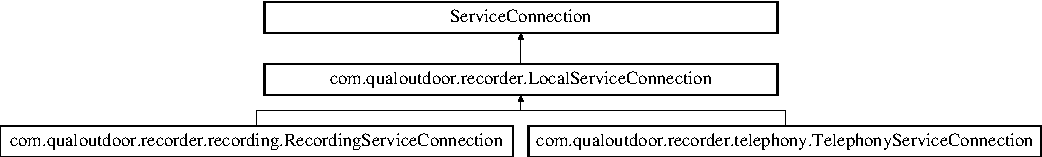
\includegraphics[height=2.115869cm]{classcom_1_1qualoutdoor_1_1recorder_1_1LocalServiceConnection}
\end{center}
\end{figure}
\subsection*{Public Member Functions}
\begin{DoxyCompactItemize}
\item 
boolean \hyperlink{classcom_1_1qualoutdoor_1_1recorder_1_1LocalServiceConnection_a1267eb452e2a476031e0b9e7ca4e2237}{is\-Bound} ()
\item 
\hypertarget{classcom_1_1qualoutdoor_1_1recorder_1_1LocalServiceConnection_ac9fe43df21f203386ff0a1b5ed6d70d8}{void {\bfseries on\-Service\-Disconnected} (Component\-Name service\-Name)}\label{classcom_1_1qualoutdoor_1_1recorder_1_1LocalServiceConnection_ac9fe43df21f203386ff0a1b5ed6d70d8}

\item 
\hypertarget{classcom_1_1qualoutdoor_1_1recorder_1_1LocalServiceConnection_aaf7e989ffaf6b728b887d5d11b245af8}{void {\bfseries on\-Service\-Connected} (Component\-Name service\-Name, I\-Binder binder)}\label{classcom_1_1qualoutdoor_1_1recorder_1_1LocalServiceConnection_aaf7e989ffaf6b728b887d5d11b245af8}

\item 
abstract void \hyperlink{classcom_1_1qualoutdoor_1_1recorder_1_1LocalServiceConnection_a54232b34d728f18d75c964438e3c5368}{on\-Service\-Obtained} ()
\end{DoxyCompactItemize}
\subsection*{Protected Attributes}
\begin{DoxyCompactItemize}
\item 
boolean \hyperlink{classcom_1_1qualoutdoor_1_1recorder_1_1LocalServiceConnection_a9583eb2308065d17b5929bb43065fa4b}{is\-Bound} = false
\end{DoxyCompactItemize}


\subsection{Detailed Description}
This Service\-Connection is meant to be used for connecting a component to services within the same process. Indeed we extend 

Definition at line 12 of file Local\-Service\-Connection.\-java.



\subsection{Member Function Documentation}
\hypertarget{classcom_1_1qualoutdoor_1_1recorder_1_1LocalServiceConnection_a1267eb452e2a476031e0b9e7ca4e2237}{\index{com\-::qualoutdoor\-::recorder\-::\-Local\-Service\-Connection@{com\-::qualoutdoor\-::recorder\-::\-Local\-Service\-Connection}!is\-Bound@{is\-Bound}}
\index{is\-Bound@{is\-Bound}!com::qualoutdoor::recorder::LocalServiceConnection@{com\-::qualoutdoor\-::recorder\-::\-Local\-Service\-Connection}}
\subsubsection[{is\-Bound}]{\setlength{\rightskip}{0pt plus 5cm}boolean com.\-qualoutdoor.\-recorder.\-Local\-Service\-Connection.\-is\-Bound (
\begin{DoxyParamCaption}
{}
\end{DoxyParamCaption}
)}}\label{classcom_1_1qualoutdoor_1_1recorder_1_1LocalServiceConnection_a1267eb452e2a476031e0b9e7ca4e2237}
Are we bound to the service ? 

Definition at line 17 of file Local\-Service\-Connection.\-java.

\hypertarget{classcom_1_1qualoutdoor_1_1recorder_1_1LocalServiceConnection_a54232b34d728f18d75c964438e3c5368}{\index{com\-::qualoutdoor\-::recorder\-::\-Local\-Service\-Connection@{com\-::qualoutdoor\-::recorder\-::\-Local\-Service\-Connection}!on\-Service\-Obtained@{on\-Service\-Obtained}}
\index{on\-Service\-Obtained@{on\-Service\-Obtained}!com::qualoutdoor::recorder::LocalServiceConnection@{com\-::qualoutdoor\-::recorder\-::\-Local\-Service\-Connection}}
\subsubsection[{on\-Service\-Obtained}]{\setlength{\rightskip}{0pt plus 5cm}abstract void com.\-qualoutdoor.\-recorder.\-Local\-Service\-Connection.\-on\-Service\-Obtained (
\begin{DoxyParamCaption}
{}
\end{DoxyParamCaption}
)\hspace{0.3cm}{\ttfamily [abstract]}}}\label{classcom_1_1qualoutdoor_1_1recorder_1_1LocalServiceConnection_a54232b34d728f18d75c964438e3c5368}
Called to allow the component to receive an instance of the Service directly. To be overridden in the component's implementation of Local\-Service\-Connected. 

\subsection{Member Data Documentation}
\hypertarget{classcom_1_1qualoutdoor_1_1recorder_1_1LocalServiceConnection_a9583eb2308065d17b5929bb43065fa4b}{\index{com\-::qualoutdoor\-::recorder\-::\-Local\-Service\-Connection@{com\-::qualoutdoor\-::recorder\-::\-Local\-Service\-Connection}!is\-Bound@{is\-Bound}}
\index{is\-Bound@{is\-Bound}!com::qualoutdoor::recorder::LocalServiceConnection@{com\-::qualoutdoor\-::recorder\-::\-Local\-Service\-Connection}}
\subsubsection[{is\-Bound}]{\setlength{\rightskip}{0pt plus 5cm}boolean com.\-qualoutdoor.\-recorder.\-Local\-Service\-Connection.\-is\-Bound = false\hspace{0.3cm}{\ttfamily [protected]}}}\label{classcom_1_1qualoutdoor_1_1recorder_1_1LocalServiceConnection_a9583eb2308065d17b5929bb43065fa4b}
Indicate if the service is bound or not 

Definition at line 14 of file Local\-Service\-Connection.\-java.



The documentation for this class was generated from the following file\-:\begin{DoxyCompactItemize}
\item 
src/com/qualoutdoor/recorder/Local\-Service\-Connection.\-java\end{DoxyCompactItemize}

\hypertarget{classcom_1_1qualoutdoor_1_1recorder_1_1MainActivity}{\section{com.\-qualoutdoor.\-recorder.\-Main\-Activity Class Reference}
\label{classcom_1_1qualoutdoor_1_1recorder_1_1MainActivity}\index{com.\-qualoutdoor.\-recorder.\-Main\-Activity@{com.\-qualoutdoor.\-recorder.\-Main\-Activity}}
}
Inheritance diagram for com.\-qualoutdoor.\-recorder.\-Main\-Activity\-:\begin{figure}[H]
\begin{center}
\leavevmode
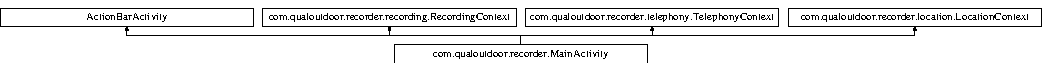
\includegraphics[height=2.000000cm]{classcom_1_1qualoutdoor_1_1recorder_1_1MainActivity}
\end{center}
\end{figure}
\subsection*{Classes}
\begin{DoxyCompactItemize}
\item 
class \hyperlink{classcom_1_1qualoutdoor_1_1recorder_1_1MainActivity_1_1DrawerItemClickListener}{Drawer\-Item\-Click\-Listener}
\end{DoxyCompactItemize}
\subsection*{Public Member Functions}
\begin{DoxyCompactItemize}
\item 
\hypertarget{classcom_1_1qualoutdoor_1_1recorder_1_1MainActivity_a05cb2528ea012100ef910ab8f594f2cf}{void {\bfseries on\-Configuration\-Changed} (Configuration new\-Config)}\label{classcom_1_1qualoutdoor_1_1recorder_1_1MainActivity_a05cb2528ea012100ef910ab8f594f2cf}

\item 
\hypertarget{classcom_1_1qualoutdoor_1_1recorder_1_1MainActivity_a07e8ec713e5d04718cf87497a7cb3dd4}{boolean {\bfseries on\-Create\-Options\-Menu} (Menu menu)}\label{classcom_1_1qualoutdoor_1_1recorder_1_1MainActivity_a07e8ec713e5d04718cf87497a7cb3dd4}

\item 
\hypertarget{classcom_1_1qualoutdoor_1_1recorder_1_1MainActivity_a03f3d576991fe48076517803a1608e42}{boolean {\bfseries on\-Prepare\-Options\-Menu} (Menu menu)}\label{classcom_1_1qualoutdoor_1_1recorder_1_1MainActivity_a03f3d576991fe48076517803a1608e42}

\item 
\hypertarget{classcom_1_1qualoutdoor_1_1recorder_1_1MainActivity_ab00ad5adc5560911e0147f3cb3cdbd50}{void {\bfseries on\-Network\-Changed} (int current\-Network, int current\-Call\-State)}\label{classcom_1_1qualoutdoor_1_1recorder_1_1MainActivity_ab00ad5adc5560911e0147f3cb3cdbd50}

\item 
\hypertarget{classcom_1_1qualoutdoor_1_1recorder_1_1MainActivity_a0788a0a3c8c1fbc9e410b94483b858b3}{boolean {\bfseries on\-Options\-Item\-Selected} (Menu\-Item item)}\label{classcom_1_1qualoutdoor_1_1recorder_1_1MainActivity_a0788a0a3c8c1fbc9e410b94483b858b3}

\item 
\hypertarget{classcom_1_1qualoutdoor_1_1recorder_1_1MainActivity_a7ab297972634760af9706e6dc8a31c92}{void {\bfseries on\-Back\-Pressed} ()}\label{classcom_1_1qualoutdoor_1_1recorder_1_1MainActivity_a7ab297972634760af9706e6dc8a31c92}

\end{DoxyCompactItemize}
\subsection*{Protected Member Functions}
\begin{DoxyCompactItemize}
\item 
void \hyperlink{classcom_1_1qualoutdoor_1_1recorder_1_1MainActivity_ac9e15af94bc29b6343dc2ffe24afe995}{on\-Create} (Bundle saved\-Instance\-State)
\item 
\hypertarget{classcom_1_1qualoutdoor_1_1recorder_1_1MainActivity_afdde657fd9139073075a608bd87250c0}{void {\bfseries on\-Post\-Create} (Bundle saved\-Instance\-State)}\label{classcom_1_1qualoutdoor_1_1recorder_1_1MainActivity_afdde657fd9139073075a608bd87250c0}

\item 
\hypertarget{classcom_1_1qualoutdoor_1_1recorder_1_1MainActivity_a465de11fed8d5c14a2ac4b458aa3985f}{void {\bfseries on\-Save\-Instance\-State} (Bundle out\-State)}\label{classcom_1_1qualoutdoor_1_1recorder_1_1MainActivity_a465de11fed8d5c14a2ac4b458aa3985f}

\item 
\hypertarget{classcom_1_1qualoutdoor_1_1recorder_1_1MainActivity_a06e1f42c4fb946ecc3a6615d6c09a7fc}{void {\bfseries on\-Start} ()}\label{classcom_1_1qualoutdoor_1_1recorder_1_1MainActivity_a06e1f42c4fb946ecc3a6615d6c09a7fc}

\item 
\hypertarget{classcom_1_1qualoutdoor_1_1recorder_1_1MainActivity_a7eb3920b7c54fc3e130c85f7f50f1c87}{void {\bfseries on\-Stop} ()}\label{classcom_1_1qualoutdoor_1_1recorder_1_1MainActivity_a7eb3920b7c54fc3e130c85f7f50f1c87}

\end{DoxyCompactItemize}
\subsection*{Private Member Functions}
\begin{DoxyCompactItemize}
\item 
void \hyperlink{classcom_1_1qualoutdoor_1_1recorder_1_1MainActivity_a70960558ff7463002c78d0f02e654263}{select\-Item} (int position)
\item 
void \hyperlink{classcom_1_1qualoutdoor_1_1recorder_1_1MainActivity_ae63f4ccd23f5892a3cea9c0c8d4aa852}{open\-Settings} ()
\item 
void \hyperlink{classcom_1_1qualoutdoor_1_1recorder_1_1MainActivity_a38c1ce314020110983c35515d9f34e48}{open\-Help} ()
\end{DoxyCompactItemize}
\subsection*{Private Attributes}
\begin{DoxyCompactItemize}
\item 
\hyperlink{classcom_1_1qualoutdoor_1_1recorder_1_1telephony_1_1TelephonyService}{Telephony\-Service} \hyperlink{classcom_1_1qualoutdoor_1_1recorder_1_1MainActivity_afa74ca8ca4d439945c9b72e360004f13}{telephony\-Service}
\item 
\hyperlink{classcom_1_1qualoutdoor_1_1recorder_1_1telephony_1_1TelephonyServiceConnection}{Telephony\-Service\-Connection} \hyperlink{classcom_1_1qualoutdoor_1_1recorder_1_1MainActivity_aee67fc3589f9ffcde9bdc275f9cdbac4}{tel\-Service\-Connection}
\item 
\hyperlink{classcom_1_1qualoutdoor_1_1recorder_1_1recording_1_1RecordingService}{Recording\-Service} \hyperlink{classcom_1_1qualoutdoor_1_1recorder_1_1MainActivity_af38fdbc2c5b036977d4e0c25d817d736}{recording\-Service}
\item 
\hyperlink{classcom_1_1qualoutdoor_1_1recorder_1_1recording_1_1RecordingServiceConnection}{Recording\-Service\-Connection} \hyperlink{classcom_1_1qualoutdoor_1_1recorder_1_1MainActivity_a672740db9e6801d1f94786f3cac1ae7a}{rec\-Service\-Connection}
\item 
Char\-Sequence \hyperlink{classcom_1_1qualoutdoor_1_1recorder_1_1MainActivity_a5959b69046a6d1ca238b4bed45b02d26}{fragment\-Title}
\item 
Char\-Sequence \hyperlink{classcom_1_1qualoutdoor_1_1recorder_1_1MainActivity_a6686ec562cfab0110bd52eddc7e33f54}{drawer\-Title}
\item 
int \hyperlink{classcom_1_1qualoutdoor_1_1recorder_1_1MainActivity_a198488a2b8d8f4d8d9b9f63939fd4dff}{active\-Section} = -\/1
\item 
String\mbox{[}$\,$\mbox{]} \hyperlink{classcom_1_1qualoutdoor_1_1recorder_1_1MainActivity_aebfe9b8493ba8495d570e4aff04aa98f}{navigation\-Titles}
\item 
Drawer\-Layout \hyperlink{classcom_1_1qualoutdoor_1_1recorder_1_1MainActivity_ad37318bd3bb05942c955bc0ccc90935d}{drawer\-Layout}
\item 
List\-View \hyperlink{classcom_1_1qualoutdoor_1_1recorder_1_1MainActivity_ab03934fd9c14fe28a6e5505d41b96cb3}{drawer\-List}
\item 
Action\-Bar\-Drawer\-Toggle \hyperlink{classcom_1_1qualoutdoor_1_1recorder_1_1MainActivity_a6c372005bb6ce12e7204e6e3729b9dab}{drawer\-Toggle}
\item 
Text\-View \hyperlink{classcom_1_1qualoutdoor_1_1recorder_1_1MainActivity_a318bc02d4937447fc88bab0f12a6df64}{network\-View}
\item 
Menu\-Item \hyperlink{classcom_1_1qualoutdoor_1_1recorder_1_1MainActivity_a76c5025a8bcde6c93e3bb320333f5d4a}{record\-Menu\-Item}
\end{DoxyCompactItemize}
\subsection*{Static Private Attributes}
\begin{DoxyCompactItemize}
\item 
static final String \hyperlink{classcom_1_1qualoutdoor_1_1recorder_1_1MainActivity_a7e719523b166c40d53fb8589b04587ab}{P\-R\-E\-V\-I\-O\-U\-S\-\_\-\-T\-I\-T\-L\-E} = \char`\"{}previous\-\_\-title\char`\"{}
\item 
static final String \hyperlink{classcom_1_1qualoutdoor_1_1recorder_1_1MainActivity_a22bb0c006feea451b77d7df1b3d8a523}{A\-C\-T\-I\-V\-E\-\_\-\-S\-E\-C\-T\-I\-O\-N} = \char`\"{}active\-\_\-section\char`\"{}
\end{DoxyCompactItemize}


\subsection{Detailed Description}


Definition at line 35 of file Main\-Activity.\-java.



\subsection{Member Function Documentation}
\hypertarget{classcom_1_1qualoutdoor_1_1recorder_1_1MainActivity_ac9e15af94bc29b6343dc2ffe24afe995}{\index{com\-::qualoutdoor\-::recorder\-::\-Main\-Activity@{com\-::qualoutdoor\-::recorder\-::\-Main\-Activity}!on\-Create@{on\-Create}}
\index{on\-Create@{on\-Create}!com::qualoutdoor::recorder::MainActivity@{com\-::qualoutdoor\-::recorder\-::\-Main\-Activity}}
\subsubsection[{on\-Create}]{\setlength{\rightskip}{0pt plus 5cm}void com.\-qualoutdoor.\-recorder.\-Main\-Activity.\-on\-Create (
\begin{DoxyParamCaption}
\item[{Bundle}]{saved\-Instance\-State}
\end{DoxyParamCaption}
)\hspace{0.3cm}{\ttfamily [protected]}}}\label{classcom_1_1qualoutdoor_1_1recorder_1_1MainActivity_ac9e15af94bc29b6343dc2ffe24afe995}
Called when a drawer has settled in a completely closed state.

Called when a drawer has settled in a completely open state. 

Definition at line 100 of file Main\-Activity.\-java.



References com.\-qualoutdoor.\-recorder.\-Main\-Activity.\-A\-C\-T\-I\-V\-E\-\_\-\-S\-E\-C\-T\-I\-O\-N, com.\-qualoutdoor.\-recorder.\-Main\-Activity.\-active\-Section, com.\-qualoutdoor.\-recorder.\-Main\-Activity.\-drawer\-Layout, com.\-qualoutdoor.\-recorder.\-Main\-Activity.\-drawer\-List, com.\-qualoutdoor.\-recorder.\-Main\-Activity.\-drawer\-Title, com.\-qualoutdoor.\-recorder.\-Main\-Activity.\-drawer\-Toggle, com.\-qualoutdoor.\-recorder.\-Main\-Activity.\-fragment\-Title, com.\-qualoutdoor.\-recorder.\-Main\-Activity.\-navigation\-Titles, com.\-qualoutdoor.\-recorder.\-Main\-Activity.\-P\-R\-E\-V\-I\-O\-U\-S\-\_\-\-T\-I\-T\-L\-E, and com.\-qualoutdoor.\-recorder.\-Main\-Activity.\-select\-Item().

\hypertarget{classcom_1_1qualoutdoor_1_1recorder_1_1MainActivity_a38c1ce314020110983c35515d9f34e48}{\index{com\-::qualoutdoor\-::recorder\-::\-Main\-Activity@{com\-::qualoutdoor\-::recorder\-::\-Main\-Activity}!open\-Help@{open\-Help}}
\index{open\-Help@{open\-Help}!com::qualoutdoor::recorder::MainActivity@{com\-::qualoutdoor\-::recorder\-::\-Main\-Activity}}
\subsubsection[{open\-Help}]{\setlength{\rightskip}{0pt plus 5cm}void com.\-qualoutdoor.\-recorder.\-Main\-Activity.\-open\-Help (
\begin{DoxyParamCaption}
{}
\end{DoxyParamCaption}
)\hspace{0.3cm}{\ttfamily [private]}}}\label{classcom_1_1qualoutdoor_1_1recorder_1_1MainActivity_a38c1ce314020110983c35515d9f34e48}
Action associated to the help option menu item 

Definition at line 422 of file Main\-Activity.\-java.

\hypertarget{classcom_1_1qualoutdoor_1_1recorder_1_1MainActivity_ae63f4ccd23f5892a3cea9c0c8d4aa852}{\index{com\-::qualoutdoor\-::recorder\-::\-Main\-Activity@{com\-::qualoutdoor\-::recorder\-::\-Main\-Activity}!open\-Settings@{open\-Settings}}
\index{open\-Settings@{open\-Settings}!com::qualoutdoor::recorder::MainActivity@{com\-::qualoutdoor\-::recorder\-::\-Main\-Activity}}
\subsubsection[{open\-Settings}]{\setlength{\rightskip}{0pt plus 5cm}void com.\-qualoutdoor.\-recorder.\-Main\-Activity.\-open\-Settings (
\begin{DoxyParamCaption}
{}
\end{DoxyParamCaption}
)\hspace{0.3cm}{\ttfamily [private]}}}\label{classcom_1_1qualoutdoor_1_1recorder_1_1MainActivity_ae63f4ccd23f5892a3cea9c0c8d4aa852}
Action associated to the settings option menu item 

Definition at line 414 of file Main\-Activity.\-java.

\hypertarget{classcom_1_1qualoutdoor_1_1recorder_1_1MainActivity_a70960558ff7463002c78d0f02e654263}{\index{com\-::qualoutdoor\-::recorder\-::\-Main\-Activity@{com\-::qualoutdoor\-::recorder\-::\-Main\-Activity}!select\-Item@{select\-Item}}
\index{select\-Item@{select\-Item}!com::qualoutdoor::recorder::MainActivity@{com\-::qualoutdoor\-::recorder\-::\-Main\-Activity}}
\subsubsection[{select\-Item}]{\setlength{\rightskip}{0pt plus 5cm}void com.\-qualoutdoor.\-recorder.\-Main\-Activity.\-select\-Item (
\begin{DoxyParamCaption}
\item[{int}]{position}
\end{DoxyParamCaption}
)\hspace{0.3cm}{\ttfamily [private]}}}\label{classcom_1_1qualoutdoor_1_1recorder_1_1MainActivity_a70960558ff7463002c78d0f02e654263}
Swaps fragments in the main content view on item selection 

Definition at line 259 of file Main\-Activity.\-java.



References com.\-qualoutdoor.\-recorder.\-Main\-Activity.\-active\-Section, com.\-qualoutdoor.\-recorder.\-Main\-Activity.\-drawer\-List, com.\-qualoutdoor.\-recorder.\-Main\-Activity.\-fragment\-Title, and com.\-qualoutdoor.\-recorder.\-Main\-Activity.\-navigation\-Titles.



Referenced by com.\-qualoutdoor.\-recorder.\-Main\-Activity.\-on\-Create().



\subsection{Member Data Documentation}
\hypertarget{classcom_1_1qualoutdoor_1_1recorder_1_1MainActivity_a22bb0c006feea451b77d7df1b3d8a523}{\index{com\-::qualoutdoor\-::recorder\-::\-Main\-Activity@{com\-::qualoutdoor\-::recorder\-::\-Main\-Activity}!A\-C\-T\-I\-V\-E\-\_\-\-S\-E\-C\-T\-I\-O\-N@{A\-C\-T\-I\-V\-E\-\_\-\-S\-E\-C\-T\-I\-O\-N}}
\index{A\-C\-T\-I\-V\-E\-\_\-\-S\-E\-C\-T\-I\-O\-N@{A\-C\-T\-I\-V\-E\-\_\-\-S\-E\-C\-T\-I\-O\-N}!com::qualoutdoor::recorder::MainActivity@{com\-::qualoutdoor\-::recorder\-::\-Main\-Activity}}
\subsubsection[{A\-C\-T\-I\-V\-E\-\_\-\-S\-E\-C\-T\-I\-O\-N}]{\setlength{\rightskip}{0pt plus 5cm}final String com.\-qualoutdoor.\-recorder.\-Main\-Activity.\-A\-C\-T\-I\-V\-E\-\_\-\-S\-E\-C\-T\-I\-O\-N = \char`\"{}active\-\_\-section\char`\"{}\hspace{0.3cm}{\ttfamily [static]}, {\ttfamily [private]}}}\label{classcom_1_1qualoutdoor_1_1recorder_1_1MainActivity_a22bb0c006feea451b77d7df1b3d8a523}
The active section key in the saved\-Instance\-State 

Definition at line 77 of file Main\-Activity.\-java.



Referenced by com.\-qualoutdoor.\-recorder.\-Main\-Activity.\-on\-Create().

\hypertarget{classcom_1_1qualoutdoor_1_1recorder_1_1MainActivity_a198488a2b8d8f4d8d9b9f63939fd4dff}{\index{com\-::qualoutdoor\-::recorder\-::\-Main\-Activity@{com\-::qualoutdoor\-::recorder\-::\-Main\-Activity}!active\-Section@{active\-Section}}
\index{active\-Section@{active\-Section}!com::qualoutdoor::recorder::MainActivity@{com\-::qualoutdoor\-::recorder\-::\-Main\-Activity}}
\subsubsection[{active\-Section}]{\setlength{\rightskip}{0pt plus 5cm}int com.\-qualoutdoor.\-recorder.\-Main\-Activity.\-active\-Section = -\/1\hspace{0.3cm}{\ttfamily [private]}}}\label{classcom_1_1qualoutdoor_1_1recorder_1_1MainActivity_a198488a2b8d8f4d8d9b9f63939fd4dff}
The active section in the navigation drawer 

Definition at line 72 of file Main\-Activity.\-java.



Referenced by com.\-qualoutdoor.\-recorder.\-Main\-Activity.\-on\-Create(), and com.\-qualoutdoor.\-recorder.\-Main\-Activity.\-select\-Item().

\hypertarget{classcom_1_1qualoutdoor_1_1recorder_1_1MainActivity_ad37318bd3bb05942c955bc0ccc90935d}{\index{com\-::qualoutdoor\-::recorder\-::\-Main\-Activity@{com\-::qualoutdoor\-::recorder\-::\-Main\-Activity}!drawer\-Layout@{drawer\-Layout}}
\index{drawer\-Layout@{drawer\-Layout}!com::qualoutdoor::recorder::MainActivity@{com\-::qualoutdoor\-::recorder\-::\-Main\-Activity}}
\subsubsection[{drawer\-Layout}]{\setlength{\rightskip}{0pt plus 5cm}Drawer\-Layout com.\-qualoutdoor.\-recorder.\-Main\-Activity.\-drawer\-Layout\hspace{0.3cm}{\ttfamily [private]}}}\label{classcom_1_1qualoutdoor_1_1recorder_1_1MainActivity_ad37318bd3bb05942c955bc0ccc90935d}
A reference to the Navigation Drawer layout 

Definition at line 82 of file Main\-Activity.\-java.



Referenced by com.\-qualoutdoor.\-recorder.\-Main\-Activity.\-on\-Create().

\hypertarget{classcom_1_1qualoutdoor_1_1recorder_1_1MainActivity_ab03934fd9c14fe28a6e5505d41b96cb3}{\index{com\-::qualoutdoor\-::recorder\-::\-Main\-Activity@{com\-::qualoutdoor\-::recorder\-::\-Main\-Activity}!drawer\-List@{drawer\-List}}
\index{drawer\-List@{drawer\-List}!com::qualoutdoor::recorder::MainActivity@{com\-::qualoutdoor\-::recorder\-::\-Main\-Activity}}
\subsubsection[{drawer\-List}]{\setlength{\rightskip}{0pt plus 5cm}List\-View com.\-qualoutdoor.\-recorder.\-Main\-Activity.\-drawer\-List\hspace{0.3cm}{\ttfamily [private]}}}\label{classcom_1_1qualoutdoor_1_1recorder_1_1MainActivity_ab03934fd9c14fe28a6e5505d41b96cb3}
The List\-View associated to the Navigation Drawer 

Definition at line 84 of file Main\-Activity.\-java.



Referenced by com.\-qualoutdoor.\-recorder.\-Main\-Activity.\-on\-Create(), and com.\-qualoutdoor.\-recorder.\-Main\-Activity.\-select\-Item().

\hypertarget{classcom_1_1qualoutdoor_1_1recorder_1_1MainActivity_a6686ec562cfab0110bd52eddc7e33f54}{\index{com\-::qualoutdoor\-::recorder\-::\-Main\-Activity@{com\-::qualoutdoor\-::recorder\-::\-Main\-Activity}!drawer\-Title@{drawer\-Title}}
\index{drawer\-Title@{drawer\-Title}!com::qualoutdoor::recorder::MainActivity@{com\-::qualoutdoor\-::recorder\-::\-Main\-Activity}}
\subsubsection[{drawer\-Title}]{\setlength{\rightskip}{0pt plus 5cm}Char\-Sequence com.\-qualoutdoor.\-recorder.\-Main\-Activity.\-drawer\-Title\hspace{0.3cm}{\ttfamily [private]}}}\label{classcom_1_1qualoutdoor_1_1recorder_1_1MainActivity_a6686ec562cfab0110bd52eddc7e33f54}
The drawer title 

Definition at line 70 of file Main\-Activity.\-java.



Referenced by com.\-qualoutdoor.\-recorder.\-Main\-Activity.\-on\-Create().

\hypertarget{classcom_1_1qualoutdoor_1_1recorder_1_1MainActivity_a6c372005bb6ce12e7204e6e3729b9dab}{\index{com\-::qualoutdoor\-::recorder\-::\-Main\-Activity@{com\-::qualoutdoor\-::recorder\-::\-Main\-Activity}!drawer\-Toggle@{drawer\-Toggle}}
\index{drawer\-Toggle@{drawer\-Toggle}!com::qualoutdoor::recorder::MainActivity@{com\-::qualoutdoor\-::recorder\-::\-Main\-Activity}}
\subsubsection[{drawer\-Toggle}]{\setlength{\rightskip}{0pt plus 5cm}Action\-Bar\-Drawer\-Toggle com.\-qualoutdoor.\-recorder.\-Main\-Activity.\-drawer\-Toggle\hspace{0.3cm}{\ttfamily [private]}}}\label{classcom_1_1qualoutdoor_1_1recorder_1_1MainActivity_a6c372005bb6ce12e7204e6e3729b9dab}
A Drawer\-Listener that integrate well with the Action\-Bar and handle the Navigation Drawer behaviors 

Definition at line 89 of file Main\-Activity.\-java.



Referenced by com.\-qualoutdoor.\-recorder.\-Main\-Activity.\-on\-Create().

\hypertarget{classcom_1_1qualoutdoor_1_1recorder_1_1MainActivity_a5959b69046a6d1ca238b4bed45b02d26}{\index{com\-::qualoutdoor\-::recorder\-::\-Main\-Activity@{com\-::qualoutdoor\-::recorder\-::\-Main\-Activity}!fragment\-Title@{fragment\-Title}}
\index{fragment\-Title@{fragment\-Title}!com::qualoutdoor::recorder::MainActivity@{com\-::qualoutdoor\-::recorder\-::\-Main\-Activity}}
\subsubsection[{fragment\-Title}]{\setlength{\rightskip}{0pt plus 5cm}Char\-Sequence com.\-qualoutdoor.\-recorder.\-Main\-Activity.\-fragment\-Title\hspace{0.3cm}{\ttfamily [private]}}}\label{classcom_1_1qualoutdoor_1_1recorder_1_1MainActivity_a5959b69046a6d1ca238b4bed45b02d26}
The current fragment title 

Definition at line 68 of file Main\-Activity.\-java.



Referenced by com.\-qualoutdoor.\-recorder.\-Main\-Activity.\-on\-Create(), and com.\-qualoutdoor.\-recorder.\-Main\-Activity.\-select\-Item().

\hypertarget{classcom_1_1qualoutdoor_1_1recorder_1_1MainActivity_aebfe9b8493ba8495d570e4aff04aa98f}{\index{com\-::qualoutdoor\-::recorder\-::\-Main\-Activity@{com\-::qualoutdoor\-::recorder\-::\-Main\-Activity}!navigation\-Titles@{navigation\-Titles}}
\index{navigation\-Titles@{navigation\-Titles}!com::qualoutdoor::recorder::MainActivity@{com\-::qualoutdoor\-::recorder\-::\-Main\-Activity}}
\subsubsection[{navigation\-Titles}]{\setlength{\rightskip}{0pt plus 5cm}String \mbox{[}$\,$\mbox{]} com.\-qualoutdoor.\-recorder.\-Main\-Activity.\-navigation\-Titles\hspace{0.3cm}{\ttfamily [private]}}}\label{classcom_1_1qualoutdoor_1_1recorder_1_1MainActivity_aebfe9b8493ba8495d570e4aff04aa98f}
Hold the navigation titles displayed in the Navigation Drawer 

Definition at line 80 of file Main\-Activity.\-java.



Referenced by com.\-qualoutdoor.\-recorder.\-Main\-Activity.\-on\-Create(), and com.\-qualoutdoor.\-recorder.\-Main\-Activity.\-select\-Item().

\hypertarget{classcom_1_1qualoutdoor_1_1recorder_1_1MainActivity_a318bc02d4937447fc88bab0f12a6df64}{\index{com\-::qualoutdoor\-::recorder\-::\-Main\-Activity@{com\-::qualoutdoor\-::recorder\-::\-Main\-Activity}!network\-View@{network\-View}}
\index{network\-View@{network\-View}!com::qualoutdoor::recorder::MainActivity@{com\-::qualoutdoor\-::recorder\-::\-Main\-Activity}}
\subsubsection[{network\-View}]{\setlength{\rightskip}{0pt plus 5cm}Text\-View com.\-qualoutdoor.\-recorder.\-Main\-Activity.\-network\-View\hspace{0.3cm}{\ttfamily [private]}}}\label{classcom_1_1qualoutdoor_1_1recorder_1_1MainActivity_a318bc02d4937447fc88bab0f12a6df64}
The view located in the action bar which displays the current network type 

Definition at line 95 of file Main\-Activity.\-java.

\hypertarget{classcom_1_1qualoutdoor_1_1recorder_1_1MainActivity_a7e719523b166c40d53fb8589b04587ab}{\index{com\-::qualoutdoor\-::recorder\-::\-Main\-Activity@{com\-::qualoutdoor\-::recorder\-::\-Main\-Activity}!P\-R\-E\-V\-I\-O\-U\-S\-\_\-\-T\-I\-T\-L\-E@{P\-R\-E\-V\-I\-O\-U\-S\-\_\-\-T\-I\-T\-L\-E}}
\index{P\-R\-E\-V\-I\-O\-U\-S\-\_\-\-T\-I\-T\-L\-E@{P\-R\-E\-V\-I\-O\-U\-S\-\_\-\-T\-I\-T\-L\-E}!com::qualoutdoor::recorder::MainActivity@{com\-::qualoutdoor\-::recorder\-::\-Main\-Activity}}
\subsubsection[{P\-R\-E\-V\-I\-O\-U\-S\-\_\-\-T\-I\-T\-L\-E}]{\setlength{\rightskip}{0pt plus 5cm}final String com.\-qualoutdoor.\-recorder.\-Main\-Activity.\-P\-R\-E\-V\-I\-O\-U\-S\-\_\-\-T\-I\-T\-L\-E = \char`\"{}previous\-\_\-title\char`\"{}\hspace{0.3cm}{\ttfamily [static]}, {\ttfamily [private]}}}\label{classcom_1_1qualoutdoor_1_1recorder_1_1MainActivity_a7e719523b166c40d53fb8589b04587ab}
The previous actionbar title key in the saved\-Instance\-State 

Definition at line 75 of file Main\-Activity.\-java.



Referenced by com.\-qualoutdoor.\-recorder.\-Main\-Activity.\-on\-Create().

\hypertarget{classcom_1_1qualoutdoor_1_1recorder_1_1MainActivity_af38fdbc2c5b036977d4e0c25d817d736}{\index{com\-::qualoutdoor\-::recorder\-::\-Main\-Activity@{com\-::qualoutdoor\-::recorder\-::\-Main\-Activity}!recording\-Service@{recording\-Service}}
\index{recording\-Service@{recording\-Service}!com::qualoutdoor::recorder::MainActivity@{com\-::qualoutdoor\-::recorder\-::\-Main\-Activity}}
\subsubsection[{recording\-Service}]{\setlength{\rightskip}{0pt plus 5cm}{\bf Recording\-Service} com.\-qualoutdoor.\-recorder.\-Main\-Activity.\-recording\-Service\hspace{0.3cm}{\ttfamily [private]}}}\label{classcom_1_1qualoutdoor_1_1recorder_1_1MainActivity_af38fdbc2c5b036977d4e0c25d817d736}
A reference to the Recording\-Service 

Definition at line 57 of file Main\-Activity.\-java.

\hypertarget{classcom_1_1qualoutdoor_1_1recorder_1_1MainActivity_a76c5025a8bcde6c93e3bb320333f5d4a}{\index{com\-::qualoutdoor\-::recorder\-::\-Main\-Activity@{com\-::qualoutdoor\-::recorder\-::\-Main\-Activity}!record\-Menu\-Item@{record\-Menu\-Item}}
\index{record\-Menu\-Item@{record\-Menu\-Item}!com::qualoutdoor::recorder::MainActivity@{com\-::qualoutdoor\-::recorder\-::\-Main\-Activity}}
\subsubsection[{record\-Menu\-Item}]{\setlength{\rightskip}{0pt plus 5cm}Menu\-Item com.\-qualoutdoor.\-recorder.\-Main\-Activity.\-record\-Menu\-Item\hspace{0.3cm}{\ttfamily [private]}}}\label{classcom_1_1qualoutdoor_1_1recorder_1_1MainActivity_a76c5025a8bcde6c93e3bb320333f5d4a}
The record action from the options menu 

Definition at line 97 of file Main\-Activity.\-java.

\hypertarget{classcom_1_1qualoutdoor_1_1recorder_1_1MainActivity_a672740db9e6801d1f94786f3cac1ae7a}{\index{com\-::qualoutdoor\-::recorder\-::\-Main\-Activity@{com\-::qualoutdoor\-::recorder\-::\-Main\-Activity}!rec\-Service\-Connection@{rec\-Service\-Connection}}
\index{rec\-Service\-Connection@{rec\-Service\-Connection}!com::qualoutdoor::recorder::MainActivity@{com\-::qualoutdoor\-::recorder\-::\-Main\-Activity}}
\subsubsection[{rec\-Service\-Connection}]{\setlength{\rightskip}{0pt plus 5cm}{\bf Recording\-Service\-Connection} com.\-qualoutdoor.\-recorder.\-Main\-Activity.\-rec\-Service\-Connection\hspace{0.3cm}{\ttfamily [private]}}}\label{classcom_1_1qualoutdoor_1_1recorder_1_1MainActivity_a672740db9e6801d1f94786f3cac1ae7a}
{\bfseries Initial value\-:}
\begin{DoxyCode}
= \textcolor{keyword}{new} RecordingServiceConnection() \{
        @Override
        \textcolor{keyword}{public} \textcolor{keywordtype}{void} onServiceObtained() \{
            
            MainActivity.this.recordingService = this.getService();
        \}
    \}
\end{DoxyCode}
The Telephony\-Service\-Connection used to connect to the Telephony\-Service 

Definition at line 59 of file Main\-Activity.\-java.

\hypertarget{classcom_1_1qualoutdoor_1_1recorder_1_1MainActivity_afa74ca8ca4d439945c9b72e360004f13}{\index{com\-::qualoutdoor\-::recorder\-::\-Main\-Activity@{com\-::qualoutdoor\-::recorder\-::\-Main\-Activity}!telephony\-Service@{telephony\-Service}}
\index{telephony\-Service@{telephony\-Service}!com::qualoutdoor::recorder::MainActivity@{com\-::qualoutdoor\-::recorder\-::\-Main\-Activity}}
\subsubsection[{telephony\-Service}]{\setlength{\rightskip}{0pt plus 5cm}{\bf Telephony\-Service} com.\-qualoutdoor.\-recorder.\-Main\-Activity.\-telephony\-Service\hspace{0.3cm}{\ttfamily [private]}}}\label{classcom_1_1qualoutdoor_1_1recorder_1_1MainActivity_afa74ca8ca4d439945c9b72e360004f13}
A reference to the Telephony\-Service 

Definition at line 46 of file Main\-Activity.\-java.

\hypertarget{classcom_1_1qualoutdoor_1_1recorder_1_1MainActivity_aee67fc3589f9ffcde9bdc275f9cdbac4}{\index{com\-::qualoutdoor\-::recorder\-::\-Main\-Activity@{com\-::qualoutdoor\-::recorder\-::\-Main\-Activity}!tel\-Service\-Connection@{tel\-Service\-Connection}}
\index{tel\-Service\-Connection@{tel\-Service\-Connection}!com::qualoutdoor::recorder::MainActivity@{com\-::qualoutdoor\-::recorder\-::\-Main\-Activity}}
\subsubsection[{tel\-Service\-Connection}]{\setlength{\rightskip}{0pt plus 5cm}{\bf Telephony\-Service\-Connection} com.\-qualoutdoor.\-recorder.\-Main\-Activity.\-tel\-Service\-Connection\hspace{0.3cm}{\ttfamily [private]}}}\label{classcom_1_1qualoutdoor_1_1recorder_1_1MainActivity_aee67fc3589f9ffcde9bdc275f9cdbac4}
{\bfseries Initial value\-:}
\begin{DoxyCode}
= \textcolor{keyword}{new} TelephonyServiceConnection() \{
        @Override
        \textcolor{keyword}{public} \textcolor{keywordtype}{void} onServiceObtained() \{
            
            MainActivity.this.telephonyService = this.getService();
        \}
    \}
\end{DoxyCode}
The Telephony\-Service\-Connection used to connect to the Telephony\-Service 

Definition at line 48 of file Main\-Activity.\-java.



The documentation for this class was generated from the following file\-:\begin{DoxyCompactItemize}
\item 
src/com/qualoutdoor/recorder/Main\-Activity.\-java\end{DoxyCompactItemize}

\hypertarget{classcom_1_1qualoutdoor_1_1recorder_1_1charting_1_1SignalStrengthSampler_1_1MyPhoneStateListener}{\section{com.\-qualoutdoor.\-recorder.\-charting.\-Signal\-Strength\-Sampler.\-My\-Phone\-State\-Listener Class Reference}
\label{classcom_1_1qualoutdoor_1_1recorder_1_1charting_1_1SignalStrengthSampler_1_1MyPhoneStateListener}\index{com.\-qualoutdoor.\-recorder.\-charting.\-Signal\-Strength\-Sampler.\-My\-Phone\-State\-Listener@{com.\-qualoutdoor.\-recorder.\-charting.\-Signal\-Strength\-Sampler.\-My\-Phone\-State\-Listener}}
}
Inheritance diagram for com.\-qualoutdoor.\-recorder.\-charting.\-Signal\-Strength\-Sampler.\-My\-Phone\-State\-Listener\-:\begin{figure}[H]
\begin{center}
\leavevmode
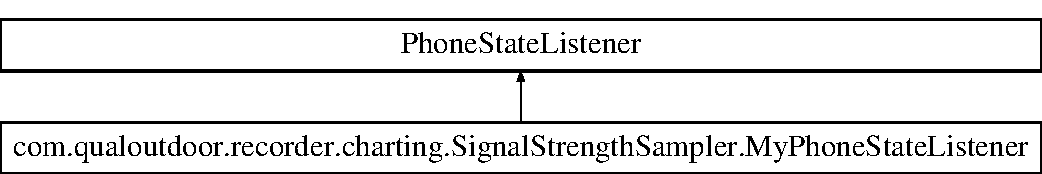
\includegraphics[height=2.000000cm]{classcom_1_1qualoutdoor_1_1recorder_1_1charting_1_1SignalStrengthSampler_1_1MyPhoneStateListener}
\end{center}
\end{figure}
\subsection*{Public Member Functions}
\begin{DoxyCompactItemize}
\item 
\hypertarget{classcom_1_1qualoutdoor_1_1recorder_1_1charting_1_1SignalStrengthSampler_1_1MyPhoneStateListener_a688de7dc88ac8f32892425e9c4663aad}{synchronized void {\bfseries on\-Signal\-Strengths\-Changed} (Signal\-Strength signal\-Strength)}\label{classcom_1_1qualoutdoor_1_1recorder_1_1charting_1_1SignalStrengthSampler_1_1MyPhoneStateListener_a688de7dc88ac8f32892425e9c4663aad}

\end{DoxyCompactItemize}


\subsection{Detailed Description}


Definition at line 12 of file Signal\-Strength\-Sampler.\-java.



The documentation for this class was generated from the following file\-:\begin{DoxyCompactItemize}
\item 
src/com/qualoutdoor/recorder/charting/Signal\-Strength\-Sampler.\-java\end{DoxyCompactItemize}

\hypertarget{classcom_1_1qualoutdoor_1_1recorder_1_1charting_1_1SignalStrengthPlotFragment_1_1MyPlotUpdater}{\section{com.\-qualoutdoor.\-recorder.\-charting.\-Signal\-Strength\-Plot\-Fragment.\-My\-Plot\-Updater Class Reference}
\label{classcom_1_1qualoutdoor_1_1recorder_1_1charting_1_1SignalStrengthPlotFragment_1_1MyPlotUpdater}\index{com.\-qualoutdoor.\-recorder.\-charting.\-Signal\-Strength\-Plot\-Fragment.\-My\-Plot\-Updater@{com.\-qualoutdoor.\-recorder.\-charting.\-Signal\-Strength\-Plot\-Fragment.\-My\-Plot\-Updater}}
}
Inheritance diagram for com.\-qualoutdoor.\-recorder.\-charting.\-Signal\-Strength\-Plot\-Fragment.\-My\-Plot\-Updater\-:\begin{figure}[H]
\begin{center}
\leavevmode
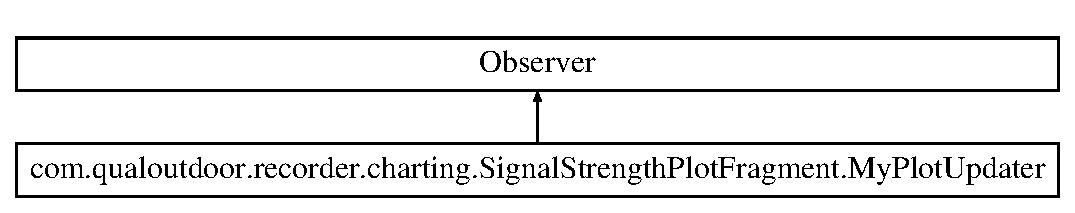
\includegraphics[height=2.000000cm]{classcom_1_1qualoutdoor_1_1recorder_1_1charting_1_1SignalStrengthPlotFragment_1_1MyPlotUpdater}
\end{center}
\end{figure}
\subsection*{Public Member Functions}
\begin{DoxyCompactItemize}
\item 
\hypertarget{classcom_1_1qualoutdoor_1_1recorder_1_1charting_1_1SignalStrengthPlotFragment_1_1MyPlotUpdater_acd5730b92572c862a7b2385e1e79ee17}{{\bfseries My\-Plot\-Updater} (Plot plot, Simple\-X\-Y\-Series series)}\label{classcom_1_1qualoutdoor_1_1recorder_1_1charting_1_1SignalStrengthPlotFragment_1_1MyPlotUpdater_acd5730b92572c862a7b2385e1e79ee17}

\item 
\hypertarget{classcom_1_1qualoutdoor_1_1recorder_1_1charting_1_1SignalStrengthPlotFragment_1_1MyPlotUpdater_ac8a7043ac6fac3a20c284ba929340e00}{void {\bfseries update} (Observable o, Object arg)}\label{classcom_1_1qualoutdoor_1_1recorder_1_1charting_1_1SignalStrengthPlotFragment_1_1MyPlotUpdater_ac8a7043ac6fac3a20c284ba929340e00}

\end{DoxyCompactItemize}


\subsection{Detailed Description}


Definition at line 33 of file Signal\-Strength\-Plot\-Fragment.\-java.



The documentation for this class was generated from the following file\-:\begin{DoxyCompactItemize}
\item 
src/com/qualoutdoor/recorder/charting/Signal\-Strength\-Plot\-Fragment.\-java\end{DoxyCompactItemize}

\hypertarget{classcom_1_1qualoutdoor_1_1recorder_1_1NavigationDrawerBehavior}{\section{com.\-qualoutdoor.\-recorder.\-Navigation\-Drawer\-Behavior Class Reference}
\label{classcom_1_1qualoutdoor_1_1recorder_1_1NavigationDrawerBehavior}\index{com.\-qualoutdoor.\-recorder.\-Navigation\-Drawer\-Behavior@{com.\-qualoutdoor.\-recorder.\-Navigation\-Drawer\-Behavior}}
}
\subsection*{Static Public Member Functions}
\begin{DoxyCompactItemize}
\item 
static Fragment \hyperlink{classcom_1_1qualoutdoor_1_1recorder_1_1NavigationDrawerBehavior_a56dc43a69769960a5d12f05e0c89abdd}{get\-Fragment} (int item\-Position)
\end{DoxyCompactItemize}
\subsection*{Static Public Attributes}
\begin{DoxyCompactItemize}
\item 
\hypertarget{classcom_1_1qualoutdoor_1_1recorder_1_1NavigationDrawerBehavior_a71fe6af02c85ff204a66b60abe212024}{static final int {\bfseries O\-V\-E\-R\-V\-I\-E\-W} = 0}\label{classcom_1_1qualoutdoor_1_1recorder_1_1NavigationDrawerBehavior_a71fe6af02c85ff204a66b60abe212024}

\item 
\hypertarget{classcom_1_1qualoutdoor_1_1recorder_1_1NavigationDrawerBehavior_aebe294104d68571c1eb4ce9af9d65178}{static final int {\bfseries M\-A\-P} = 1}\label{classcom_1_1qualoutdoor_1_1recorder_1_1NavigationDrawerBehavior_aebe294104d68571c1eb4ce9af9d65178}

\item 
\hypertarget{classcom_1_1qualoutdoor_1_1recorder_1_1NavigationDrawerBehavior_a8368f632c82d3eff9da1fc2e729c2bce}{static final int {\bfseries S\-T\-A\-T\-I\-S\-T\-I\-C\-S} = 2}\label{classcom_1_1qualoutdoor_1_1recorder_1_1NavigationDrawerBehavior_a8368f632c82d3eff9da1fc2e729c2bce}

\item 
\hypertarget{classcom_1_1qualoutdoor_1_1recorder_1_1NavigationDrawerBehavior_adfb5f8a3ab94d190d16e7dfb5004dc4b}{static final int {\bfseries S\-C\-R\-I\-P\-T\-S} = 3}\label{classcom_1_1qualoutdoor_1_1recorder_1_1NavigationDrawerBehavior_adfb5f8a3ab94d190d16e7dfb5004dc4b}

\end{DoxyCompactItemize}


\subsection{Detailed Description}
This class define the order and the association between items in the Navigation Drawer and their corresponding fragments 

Definition at line 14 of file Navigation\-Drawer\-Behavior.\-java.



\subsection{Member Function Documentation}
\hypertarget{classcom_1_1qualoutdoor_1_1recorder_1_1NavigationDrawerBehavior_a56dc43a69769960a5d12f05e0c89abdd}{\index{com\-::qualoutdoor\-::recorder\-::\-Navigation\-Drawer\-Behavior@{com\-::qualoutdoor\-::recorder\-::\-Navigation\-Drawer\-Behavior}!get\-Fragment@{get\-Fragment}}
\index{get\-Fragment@{get\-Fragment}!com::qualoutdoor::recorder::NavigationDrawerBehavior@{com\-::qualoutdoor\-::recorder\-::\-Navigation\-Drawer\-Behavior}}
\subsubsection[{get\-Fragment}]{\setlength{\rightskip}{0pt plus 5cm}static Fragment com.\-qualoutdoor.\-recorder.\-Navigation\-Drawer\-Behavior.\-get\-Fragment (
\begin{DoxyParamCaption}
\item[{int}]{item\-Position}
\end{DoxyParamCaption}
)\hspace{0.3cm}{\ttfamily [static]}}}\label{classcom_1_1qualoutdoor_1_1recorder_1_1NavigationDrawerBehavior_a56dc43a69769960a5d12f05e0c89abdd}
Get the fragment corresponding to the given item 

Definition at line 22 of file Navigation\-Drawer\-Behavior.\-java.



The documentation for this class was generated from the following file\-:\begin{DoxyCompactItemize}
\item 
src/com/qualoutdoor/recorder/Navigation\-Drawer\-Behavior.\-java\end{DoxyCompactItemize}

\hypertarget{interfacecom_1_1qualoutdoor_1_1recorder_1_1QualOutdoorApp_1_1NetworkChangeListener}{\section{com.\-qualoutdoor.\-recorder.\-Qual\-Outdoor\-App.\-Network\-Change\-Listener Interface Reference}
\label{interfacecom_1_1qualoutdoor_1_1recorder_1_1QualOutdoorApp_1_1NetworkChangeListener}\index{com.\-qualoutdoor.\-recorder.\-Qual\-Outdoor\-App.\-Network\-Change\-Listener@{com.\-qualoutdoor.\-recorder.\-Qual\-Outdoor\-App.\-Network\-Change\-Listener}}
}
\subsection*{Public Member Functions}
\begin{DoxyCompactItemize}
\item 
\hypertarget{interfacecom_1_1qualoutdoor_1_1recorder_1_1QualOutdoorApp_1_1NetworkChangeListener_a9c52b2774b1c63474c5eed3ce703e168}{void {\bfseries on\-Network\-Changed} (int network, int call\-State)}\label{interfacecom_1_1qualoutdoor_1_1recorder_1_1QualOutdoorApp_1_1NetworkChangeListener_a9c52b2774b1c63474c5eed3ce703e168}

\end{DoxyCompactItemize}


\subsection{Detailed Description}
An interface for network changes listeners 

Definition at line 17 of file Qual\-Outdoor\-App.\-java.



The documentation for this interface was generated from the following file\-:\begin{DoxyCompactItemize}
\item 
src/com/qualoutdoor/recorder/Qual\-Outdoor\-App.\-java\end{DoxyCompactItemize}

\hypertarget{classcom_1_1qualoutdoor_1_1recorder_1_1notifications_1_1NotificationCenter}{\section{com.\-qualoutdoor.\-recorder.\-notifications.\-Notification\-Center Class Reference}
\label{classcom_1_1qualoutdoor_1_1recorder_1_1notifications_1_1NotificationCenter}\index{com.\-qualoutdoor.\-recorder.\-notifications.\-Notification\-Center@{com.\-qualoutdoor.\-recorder.\-notifications.\-Notification\-Center}}
}
\subsection*{Static Public Member Functions}
\begin{DoxyCompactItemize}
\item 
static Notification \hyperlink{classcom_1_1qualoutdoor_1_1recorder_1_1notifications_1_1NotificationCenter_a594d7753e910b1eb8782e2e8a3601ae1}{get\-Recording\-Notification} (Context context)
\item 
static void \hyperlink{classcom_1_1qualoutdoor_1_1recorder_1_1notifications_1_1NotificationCenter_a42f3211ad67cfa311b3d5d81f31f370f}{notify\-Background\-Recording} (Context context)
\item 
\hypertarget{classcom_1_1qualoutdoor_1_1recorder_1_1notifications_1_1NotificationCenter_ad0032647617b97a891df182533d8fb5c}{static void {\bfseries dismiss\-Background\-Recording} (Context context)}\label{classcom_1_1qualoutdoor_1_1recorder_1_1notifications_1_1NotificationCenter_ad0032647617b97a891df182533d8fb5c}

\end{DoxyCompactItemize}
\subsection*{Static Public Attributes}
\begin{DoxyCompactItemize}
\item 
static final int \hyperlink{classcom_1_1qualoutdoor_1_1recorder_1_1notifications_1_1NotificationCenter_a1316ea946cb84d237c20e491c363cd33}{B\-A\-C\-K\-G\-R\-O\-U\-N\-D\-\_\-\-R\-E\-C\-O\-R\-D\-I\-N\-G} = 1337
\end{DoxyCompactItemize}
\subsection*{Private Member Functions}
\begin{DoxyCompactItemize}
\item 
\hyperlink{classcom_1_1qualoutdoor_1_1recorder_1_1notifications_1_1NotificationCenter_a212d336ad0b5722e951904316b793b78}{Notification\-Center} ()
\end{DoxyCompactItemize}


\subsection{Detailed Description}
This class is a utility class allowing the app to manage user notifications. An exemple of notification is the \char`\"{}ongoing recording\char`\"{} notification which tells the user that the app is currently recording 

Definition at line 20 of file Notification\-Center.\-java.



\subsection{Constructor \& Destructor Documentation}
\hypertarget{classcom_1_1qualoutdoor_1_1recorder_1_1notifications_1_1NotificationCenter_a212d336ad0b5722e951904316b793b78}{\index{com\-::qualoutdoor\-::recorder\-::notifications\-::\-Notification\-Center@{com\-::qualoutdoor\-::recorder\-::notifications\-::\-Notification\-Center}!Notification\-Center@{Notification\-Center}}
\index{Notification\-Center@{Notification\-Center}!com::qualoutdoor::recorder::notifications::NotificationCenter@{com\-::qualoutdoor\-::recorder\-::notifications\-::\-Notification\-Center}}
\subsubsection[{Notification\-Center}]{\setlength{\rightskip}{0pt plus 5cm}com.\-qualoutdoor.\-recorder.\-notifications.\-Notification\-Center.\-Notification\-Center (
\begin{DoxyParamCaption}
{}
\end{DoxyParamCaption}
)\hspace{0.3cm}{\ttfamily [private]}}}\label{classcom_1_1qualoutdoor_1_1recorder_1_1notifications_1_1NotificationCenter_a212d336ad0b5722e951904316b793b78}
This class is not meant to be instantiated 

Definition at line 26 of file Notification\-Center.\-java.



\subsection{Member Function Documentation}
\hypertarget{classcom_1_1qualoutdoor_1_1recorder_1_1notifications_1_1NotificationCenter_a594d7753e910b1eb8782e2e8a3601ae1}{\index{com\-::qualoutdoor\-::recorder\-::notifications\-::\-Notification\-Center@{com\-::qualoutdoor\-::recorder\-::notifications\-::\-Notification\-Center}!get\-Recording\-Notification@{get\-Recording\-Notification}}
\index{get\-Recording\-Notification@{get\-Recording\-Notification}!com::qualoutdoor::recorder::notifications::NotificationCenter@{com\-::qualoutdoor\-::recorder\-::notifications\-::\-Notification\-Center}}
\subsubsection[{get\-Recording\-Notification}]{\setlength{\rightskip}{0pt plus 5cm}static Notification com.\-qualoutdoor.\-recorder.\-notifications.\-Notification\-Center.\-get\-Recording\-Notification (
\begin{DoxyParamCaption}
\item[{Context}]{context}
\end{DoxyParamCaption}
)\hspace{0.3cm}{\ttfamily [static]}}}\label{classcom_1_1qualoutdoor_1_1recorder_1_1notifications_1_1NotificationCenter_a594d7753e910b1eb8782e2e8a3601ae1}
Obtain a notification corresponding to an ongoing recording process 

Definition at line 30 of file Notification\-Center.\-java.



Referenced by com.\-qualoutdoor.\-recorder.\-notifications.\-Notification\-Center.\-notify\-Background\-Recording().

\hypertarget{classcom_1_1qualoutdoor_1_1recorder_1_1notifications_1_1NotificationCenter_a42f3211ad67cfa311b3d5d81f31f370f}{\index{com\-::qualoutdoor\-::recorder\-::notifications\-::\-Notification\-Center@{com\-::qualoutdoor\-::recorder\-::notifications\-::\-Notification\-Center}!notify\-Background\-Recording@{notify\-Background\-Recording}}
\index{notify\-Background\-Recording@{notify\-Background\-Recording}!com::qualoutdoor::recorder::notifications::NotificationCenter@{com\-::qualoutdoor\-::recorder\-::notifications\-::\-Notification\-Center}}
\subsubsection[{notify\-Background\-Recording}]{\setlength{\rightskip}{0pt plus 5cm}static void com.\-qualoutdoor.\-recorder.\-notifications.\-Notification\-Center.\-notify\-Background\-Recording (
\begin{DoxyParamCaption}
\item[{Context}]{context}
\end{DoxyParamCaption}
)\hspace{0.3cm}{\ttfamily [static]}}}\label{classcom_1_1qualoutdoor_1_1recorder_1_1notifications_1_1NotificationCenter_a42f3211ad67cfa311b3d5d81f31f370f}
Switch on/off the ongoing recording notification 

Definition at line 71 of file Notification\-Center.\-java.



References com.\-qualoutdoor.\-recorder.\-notifications.\-Notification\-Center.\-B\-A\-C\-K\-G\-R\-O\-U\-N\-D\-\_\-\-R\-E\-C\-O\-R\-D\-I\-N\-G, and com.\-qualoutdoor.\-recorder.\-notifications.\-Notification\-Center.\-get\-Recording\-Notification().



\subsection{Member Data Documentation}
\hypertarget{classcom_1_1qualoutdoor_1_1recorder_1_1notifications_1_1NotificationCenter_a1316ea946cb84d237c20e491c363cd33}{\index{com\-::qualoutdoor\-::recorder\-::notifications\-::\-Notification\-Center@{com\-::qualoutdoor\-::recorder\-::notifications\-::\-Notification\-Center}!B\-A\-C\-K\-G\-R\-O\-U\-N\-D\-\_\-\-R\-E\-C\-O\-R\-D\-I\-N\-G@{B\-A\-C\-K\-G\-R\-O\-U\-N\-D\-\_\-\-R\-E\-C\-O\-R\-D\-I\-N\-G}}
\index{B\-A\-C\-K\-G\-R\-O\-U\-N\-D\-\_\-\-R\-E\-C\-O\-R\-D\-I\-N\-G@{B\-A\-C\-K\-G\-R\-O\-U\-N\-D\-\_\-\-R\-E\-C\-O\-R\-D\-I\-N\-G}!com::qualoutdoor::recorder::notifications::NotificationCenter@{com\-::qualoutdoor\-::recorder\-::notifications\-::\-Notification\-Center}}
\subsubsection[{B\-A\-C\-K\-G\-R\-O\-U\-N\-D\-\_\-\-R\-E\-C\-O\-R\-D\-I\-N\-G}]{\setlength{\rightskip}{0pt plus 5cm}final int com.\-qualoutdoor.\-recorder.\-notifications.\-Notification\-Center.\-B\-A\-C\-K\-G\-R\-O\-U\-N\-D\-\_\-\-R\-E\-C\-O\-R\-D\-I\-N\-G = 1337\hspace{0.3cm}{\ttfamily [static]}}}\label{classcom_1_1qualoutdoor_1_1recorder_1_1notifications_1_1NotificationCenter_a1316ea946cb84d237c20e491c363cd33}
The id of the background recording notification 

Definition at line 23 of file Notification\-Center.\-java.



Referenced by com.\-qualoutdoor.\-recorder.\-notifications.\-Notification\-Center.\-notify\-Background\-Recording(), and com.\-qualoutdoor.\-recorder.\-recording.\-Recording\-Service.\-start\-Recording().



The documentation for this class was generated from the following file\-:\begin{DoxyCompactItemize}
\item 
src/com/qualoutdoor/recorder/notifications/Notification\-Center.\-java\end{DoxyCompactItemize}

\hypertarget{classcom_1_1qualoutdoor_1_1recorder_1_1OverviewFragment}{\section{com.\-qualoutdoor.\-recorder.\-Overview\-Fragment Class Reference}
\label{classcom_1_1qualoutdoor_1_1recorder_1_1OverviewFragment}\index{com.\-qualoutdoor.\-recorder.\-Overview\-Fragment@{com.\-qualoutdoor.\-recorder.\-Overview\-Fragment}}
}
Inheritance diagram for com.\-qualoutdoor.\-recorder.\-Overview\-Fragment\-:\begin{figure}[H]
\begin{center}
\leavevmode
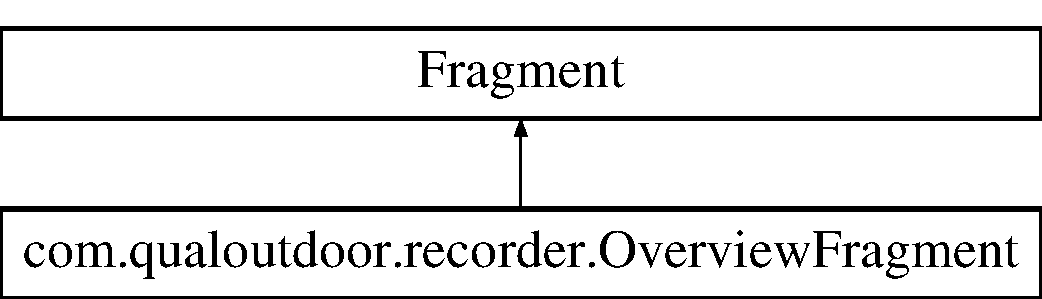
\includegraphics[height=2.000000cm]{classcom_1_1qualoutdoor_1_1recorder_1_1OverviewFragment}
\end{center}
\end{figure}
\subsection*{Public Member Functions}
\begin{DoxyCompactItemize}
\item 
\hypertarget{classcom_1_1qualoutdoor_1_1recorder_1_1OverviewFragment_ab0fd9f82a732308d4e6595d6708c58d7}{View {\bfseries on\-Create\-View} (Layout\-Inflater inflater, View\-Group container, Bundle saved\-Instance\-State)}\label{classcom_1_1qualoutdoor_1_1recorder_1_1OverviewFragment_ab0fd9f82a732308d4e6595d6708c58d7}

\end{DoxyCompactItemize}


\subsection{Detailed Description}


Definition at line 9 of file Overview\-Fragment.\-java.



The documentation for this class was generated from the following file\-:\begin{DoxyCompactItemize}
\item 
src/com/qualoutdoor/recorder/Overview\-Fragment.\-java\end{DoxyCompactItemize}

\hypertarget{classcom_1_1qualoutdoor_1_1recorder_1_1QualOutdoorApp}{\section{com.\-qualoutdoor.\-recorder.\-Qual\-Outdoor\-App Class Reference}
\label{classcom_1_1qualoutdoor_1_1recorder_1_1QualOutdoorApp}\index{com.\-qualoutdoor.\-recorder.\-Qual\-Outdoor\-App@{com.\-qualoutdoor.\-recorder.\-Qual\-Outdoor\-App}}
}
Inheritance diagram for com.\-qualoutdoor.\-recorder.\-Qual\-Outdoor\-App\-:\begin{figure}[H]
\begin{center}
\leavevmode
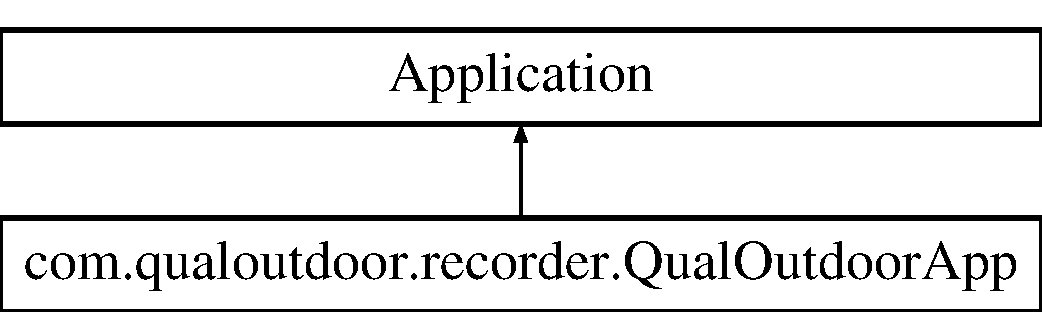
\includegraphics[height=2.000000cm]{classcom_1_1qualoutdoor_1_1recorder_1_1QualOutdoorApp}
\end{center}
\end{figure}
\subsection*{Classes}
\begin{DoxyCompactItemize}
\item 
interface \hyperlink{interfacecom_1_1qualoutdoor_1_1recorder_1_1QualOutdoorApp_1_1NetworkChangeListener}{Network\-Change\-Listener}
\end{DoxyCompactItemize}
\subsection*{Public Member Functions}
\begin{DoxyCompactItemize}
\item 
\hyperlink{classcom_1_1qualoutdoor_1_1recorder_1_1QualOutdoorApp_a863e6a3fe7d020d62629cc47049a5618}{Qual\-Outdoor\-App} ()
\item 
int \hyperlink{classcom_1_1qualoutdoor_1_1recorder_1_1QualOutdoorApp_ac9fdf8864e00f880803658ef94e8f20b}{get\-Current\-Network} ()
\item 
void \hyperlink{classcom_1_1qualoutdoor_1_1recorder_1_1QualOutdoorApp_a8d02d25c00d87540548e55b1de410b60}{set\-Current\-Network} (int network)
\item 
int \hyperlink{classcom_1_1qualoutdoor_1_1recorder_1_1QualOutdoorApp_a1d011e7d39b12c3657b5a927fda0ea8f}{get\-Call\-State} ()
\item 
void \hyperlink{classcom_1_1qualoutdoor_1_1recorder_1_1QualOutdoorApp_a195cc6939ad7d5d2dd8aae046ae8fb6a}{set\-Call\-State} (int call\-State)
\item 
void \hyperlink{classcom_1_1qualoutdoor_1_1recorder_1_1QualOutdoorApp_a829786bb3de92bfc6f38ed85d04aa44e}{add\-Network\-Change\-Listener} (\hyperlink{interfacecom_1_1qualoutdoor_1_1recorder_1_1QualOutdoorApp_1_1NetworkChangeListener}{Network\-Change\-Listener} l)
\item 
void \hyperlink{classcom_1_1qualoutdoor_1_1recorder_1_1QualOutdoorApp_a34ce4fb04563b6f5f808866ec9156ac8}{remove\-Network\-Change\-Listener} (\hyperlink{interfacecom_1_1qualoutdoor_1_1recorder_1_1QualOutdoorApp_1_1NetworkChangeListener}{Network\-Change\-Listener} l)
\item 
void \hyperlink{classcom_1_1qualoutdoor_1_1recorder_1_1QualOutdoorApp_a3d9228b4b2a55f80718d82d53fd6ca8c}{notify\-Network\-Listeners} (int current\-Network, int current\-Call\-State)
\item 
boolean \hyperlink{classcom_1_1qualoutdoor_1_1recorder_1_1QualOutdoorApp_a9ab899682caf9bc4eafa3bf236f9b4e4}{is\-Recording} ()
\item 
void \hyperlink{classcom_1_1qualoutdoor_1_1recorder_1_1QualOutdoorApp_af8b76cf31bccb966036a94a3cbe086e1}{switch\-Recording} ()
\item 
void \hyperlink{classcom_1_1qualoutdoor_1_1recorder_1_1QualOutdoorApp_ae1aaa8d84f0e13c8448beb8901a1aafd}{notify\-Recording} ()
\end{DoxyCompactItemize}
\subsection*{Private Member Functions}
\begin{DoxyCompactItemize}
\item 
void \hyperlink{classcom_1_1qualoutdoor_1_1recorder_1_1QualOutdoorApp_aaa95acb3101a265a6ecca3479ccd8298}{stop\-Recording} ()
\item 
void \hyperlink{classcom_1_1qualoutdoor_1_1recorder_1_1QualOutdoorApp_aa6d92737d7715f9b80a8a97c1f3c91b7}{start\-Recording} ()
\end{DoxyCompactItemize}
\subsection*{Private Attributes}
\begin{DoxyCompactItemize}
\item 
final Copy\-On\-Write\-Array\-List\\*
$<$ \hyperlink{interfacecom_1_1qualoutdoor_1_1recorder_1_1QualOutdoorApp_1_1NetworkChangeListener}{Network\-Change\-Listener} $>$ \hyperlink{classcom_1_1qualoutdoor_1_1recorder_1_1QualOutdoorApp_a355e77531ef176519c95f6d179a97889}{network\-Listeners}
\item 
\hypertarget{classcom_1_1qualoutdoor_1_1recorder_1_1QualOutdoorApp_a723c6a6184bda3f001148ae37fc3f230}{int {\bfseries current\-Network} = Telephony\-Manager.\-N\-E\-T\-W\-O\-R\-K\-\_\-\-T\-Y\-P\-E\-\_\-\-U\-N\-K\-N\-O\-W\-N}\label{classcom_1_1qualoutdoor_1_1recorder_1_1QualOutdoorApp_a723c6a6184bda3f001148ae37fc3f230}

\item 
\hypertarget{classcom_1_1qualoutdoor_1_1recorder_1_1QualOutdoorApp_a358eaab2d4ac7f4de7bfc440abe1d149}{int {\bfseries call\-State} = Telephony\-Manager.\-C\-A\-L\-L\-\_\-\-S\-T\-A\-T\-E\-\_\-\-I\-D\-L\-E}\label{classcom_1_1qualoutdoor_1_1recorder_1_1QualOutdoorApp_a358eaab2d4ac7f4de7bfc440abe1d149}

\item 
\hypertarget{classcom_1_1qualoutdoor_1_1recorder_1_1QualOutdoorApp_a3ccdb482ddb310afd4dcad402c513dae}{boolean {\bfseries recording} = false}\label{classcom_1_1qualoutdoor_1_1recorder_1_1QualOutdoorApp_a3ccdb482ddb310afd4dcad402c513dae}

\end{DoxyCompactItemize}


\subsection{Detailed Description}
The application class, it holds attributes and methods that are global to the application 

Definition at line 14 of file Qual\-Outdoor\-App.\-java.



\subsection{Constructor \& Destructor Documentation}
\hypertarget{classcom_1_1qualoutdoor_1_1recorder_1_1QualOutdoorApp_a863e6a3fe7d020d62629cc47049a5618}{\index{com\-::qualoutdoor\-::recorder\-::\-Qual\-Outdoor\-App@{com\-::qualoutdoor\-::recorder\-::\-Qual\-Outdoor\-App}!Qual\-Outdoor\-App@{Qual\-Outdoor\-App}}
\index{Qual\-Outdoor\-App@{Qual\-Outdoor\-App}!com::qualoutdoor::recorder::QualOutdoorApp@{com\-::qualoutdoor\-::recorder\-::\-Qual\-Outdoor\-App}}
\subsubsection[{Qual\-Outdoor\-App}]{\setlength{\rightskip}{0pt plus 5cm}com.\-qualoutdoor.\-recorder.\-Qual\-Outdoor\-App.\-Qual\-Outdoor\-App (
\begin{DoxyParamCaption}
{}
\end{DoxyParamCaption}
)}}\label{classcom_1_1qualoutdoor_1_1recorder_1_1QualOutdoorApp_a863e6a3fe7d020d62629cc47049a5618}
The application constructor 

Definition at line 36 of file Qual\-Outdoor\-App.\-java.



\subsection{Member Function Documentation}
\hypertarget{classcom_1_1qualoutdoor_1_1recorder_1_1QualOutdoorApp_a829786bb3de92bfc6f38ed85d04aa44e}{\index{com\-::qualoutdoor\-::recorder\-::\-Qual\-Outdoor\-App@{com\-::qualoutdoor\-::recorder\-::\-Qual\-Outdoor\-App}!add\-Network\-Change\-Listener@{add\-Network\-Change\-Listener}}
\index{add\-Network\-Change\-Listener@{add\-Network\-Change\-Listener}!com::qualoutdoor::recorder::QualOutdoorApp@{com\-::qualoutdoor\-::recorder\-::\-Qual\-Outdoor\-App}}
\subsubsection[{add\-Network\-Change\-Listener}]{\setlength{\rightskip}{0pt plus 5cm}void com.\-qualoutdoor.\-recorder.\-Qual\-Outdoor\-App.\-add\-Network\-Change\-Listener (
\begin{DoxyParamCaption}
\item[{{\bf Network\-Change\-Listener}}]{l}
\end{DoxyParamCaption}
)}}\label{classcom_1_1qualoutdoor_1_1recorder_1_1QualOutdoorApp_a829786bb3de92bfc6f38ed85d04aa44e}
Add a new listener 

Definition at line 65 of file Qual\-Outdoor\-App.\-java.

\hypertarget{classcom_1_1qualoutdoor_1_1recorder_1_1QualOutdoorApp_a1d011e7d39b12c3657b5a927fda0ea8f}{\index{com\-::qualoutdoor\-::recorder\-::\-Qual\-Outdoor\-App@{com\-::qualoutdoor\-::recorder\-::\-Qual\-Outdoor\-App}!get\-Call\-State@{get\-Call\-State}}
\index{get\-Call\-State@{get\-Call\-State}!com::qualoutdoor::recorder::QualOutdoorApp@{com\-::qualoutdoor\-::recorder\-::\-Qual\-Outdoor\-App}}
\subsubsection[{get\-Call\-State}]{\setlength{\rightskip}{0pt plus 5cm}int com.\-qualoutdoor.\-recorder.\-Qual\-Outdoor\-App.\-get\-Call\-State (
\begin{DoxyParamCaption}
{}
\end{DoxyParamCaption}
)}}\label{classcom_1_1qualoutdoor_1_1recorder_1_1QualOutdoorApp_a1d011e7d39b12c3657b5a927fda0ea8f}
Get the current call state 

Definition at line 54 of file Qual\-Outdoor\-App.\-java.

\hypertarget{classcom_1_1qualoutdoor_1_1recorder_1_1QualOutdoorApp_ac9fdf8864e00f880803658ef94e8f20b}{\index{com\-::qualoutdoor\-::recorder\-::\-Qual\-Outdoor\-App@{com\-::qualoutdoor\-::recorder\-::\-Qual\-Outdoor\-App}!get\-Current\-Network@{get\-Current\-Network}}
\index{get\-Current\-Network@{get\-Current\-Network}!com::qualoutdoor::recorder::QualOutdoorApp@{com\-::qualoutdoor\-::recorder\-::\-Qual\-Outdoor\-App}}
\subsubsection[{get\-Current\-Network}]{\setlength{\rightskip}{0pt plus 5cm}int com.\-qualoutdoor.\-recorder.\-Qual\-Outdoor\-App.\-get\-Current\-Network (
\begin{DoxyParamCaption}
{}
\end{DoxyParamCaption}
)}}\label{classcom_1_1qualoutdoor_1_1recorder_1_1QualOutdoorApp_ac9fdf8864e00f880803658ef94e8f20b}
Get the current network value 

Definition at line 41 of file Qual\-Outdoor\-App.\-java.

\hypertarget{classcom_1_1qualoutdoor_1_1recorder_1_1QualOutdoorApp_a9ab899682caf9bc4eafa3bf236f9b4e4}{\index{com\-::qualoutdoor\-::recorder\-::\-Qual\-Outdoor\-App@{com\-::qualoutdoor\-::recorder\-::\-Qual\-Outdoor\-App}!is\-Recording@{is\-Recording}}
\index{is\-Recording@{is\-Recording}!com::qualoutdoor::recorder::QualOutdoorApp@{com\-::qualoutdoor\-::recorder\-::\-Qual\-Outdoor\-App}}
\subsubsection[{is\-Recording}]{\setlength{\rightskip}{0pt plus 5cm}boolean com.\-qualoutdoor.\-recorder.\-Qual\-Outdoor\-App.\-is\-Recording (
\begin{DoxyParamCaption}
{}
\end{DoxyParamCaption}
)}}\label{classcom_1_1qualoutdoor_1_1recorder_1_1QualOutdoorApp_a9ab899682caf9bc4eafa3bf236f9b4e4}
Indicate if the background recording process is running 

Definition at line 84 of file Qual\-Outdoor\-App.\-java.

\hypertarget{classcom_1_1qualoutdoor_1_1recorder_1_1QualOutdoorApp_a3d9228b4b2a55f80718d82d53fd6ca8c}{\index{com\-::qualoutdoor\-::recorder\-::\-Qual\-Outdoor\-App@{com\-::qualoutdoor\-::recorder\-::\-Qual\-Outdoor\-App}!notify\-Network\-Listeners@{notify\-Network\-Listeners}}
\index{notify\-Network\-Listeners@{notify\-Network\-Listeners}!com::qualoutdoor::recorder::QualOutdoorApp@{com\-::qualoutdoor\-::recorder\-::\-Qual\-Outdoor\-App}}
\subsubsection[{notify\-Network\-Listeners}]{\setlength{\rightskip}{0pt plus 5cm}void com.\-qualoutdoor.\-recorder.\-Qual\-Outdoor\-App.\-notify\-Network\-Listeners (
\begin{DoxyParamCaption}
\item[{int}]{current\-Network, }
\item[{int}]{current\-Call\-State}
\end{DoxyParamCaption}
)}}\label{classcom_1_1qualoutdoor_1_1recorder_1_1QualOutdoorApp_a3d9228b4b2a55f80718d82d53fd6ca8c}
Notifies the network changes listeners that the network type has changed 

Definition at line 75 of file Qual\-Outdoor\-App.\-java.



References com.\-qualoutdoor.\-recorder.\-Qual\-Outdoor\-App.\-network\-Listeners.



Referenced by com.\-qualoutdoor.\-recorder.\-Qual\-Outdoor\-App.\-set\-Call\-State(), and com.\-qualoutdoor.\-recorder.\-Qual\-Outdoor\-App.\-set\-Current\-Network().

\hypertarget{classcom_1_1qualoutdoor_1_1recorder_1_1QualOutdoorApp_ae1aaa8d84f0e13c8448beb8901a1aafd}{\index{com\-::qualoutdoor\-::recorder\-::\-Qual\-Outdoor\-App@{com\-::qualoutdoor\-::recorder\-::\-Qual\-Outdoor\-App}!notify\-Recording@{notify\-Recording}}
\index{notify\-Recording@{notify\-Recording}!com::qualoutdoor::recorder::QualOutdoorApp@{com\-::qualoutdoor\-::recorder\-::\-Qual\-Outdoor\-App}}
\subsubsection[{notify\-Recording}]{\setlength{\rightskip}{0pt plus 5cm}void com.\-qualoutdoor.\-recorder.\-Qual\-Outdoor\-App.\-notify\-Recording (
\begin{DoxyParamCaption}
{}
\end{DoxyParamCaption}
)}}\label{classcom_1_1qualoutdoor_1_1recorder_1_1QualOutdoorApp_ae1aaa8d84f0e13c8448beb8901a1aafd}
Create a notification according to the recorder state 

Definition at line 112 of file Qual\-Outdoor\-App.\-java.



Referenced by com.\-qualoutdoor.\-recorder.\-Qual\-Outdoor\-App.\-start\-Recording(), and com.\-qualoutdoor.\-recorder.\-Qual\-Outdoor\-App.\-stop\-Recording().

\hypertarget{classcom_1_1qualoutdoor_1_1recorder_1_1QualOutdoorApp_a34ce4fb04563b6f5f808866ec9156ac8}{\index{com\-::qualoutdoor\-::recorder\-::\-Qual\-Outdoor\-App@{com\-::qualoutdoor\-::recorder\-::\-Qual\-Outdoor\-App}!remove\-Network\-Change\-Listener@{remove\-Network\-Change\-Listener}}
\index{remove\-Network\-Change\-Listener@{remove\-Network\-Change\-Listener}!com::qualoutdoor::recorder::QualOutdoorApp@{com\-::qualoutdoor\-::recorder\-::\-Qual\-Outdoor\-App}}
\subsubsection[{remove\-Network\-Change\-Listener}]{\setlength{\rightskip}{0pt plus 5cm}void com.\-qualoutdoor.\-recorder.\-Qual\-Outdoor\-App.\-remove\-Network\-Change\-Listener (
\begin{DoxyParamCaption}
\item[{{\bf Network\-Change\-Listener}}]{l}
\end{DoxyParamCaption}
)}}\label{classcom_1_1qualoutdoor_1_1recorder_1_1QualOutdoorApp_a34ce4fb04563b6f5f808866ec9156ac8}
Remove a listener to the list 

Definition at line 70 of file Qual\-Outdoor\-App.\-java.

\hypertarget{classcom_1_1qualoutdoor_1_1recorder_1_1QualOutdoorApp_a195cc6939ad7d5d2dd8aae046ae8fb6a}{\index{com\-::qualoutdoor\-::recorder\-::\-Qual\-Outdoor\-App@{com\-::qualoutdoor\-::recorder\-::\-Qual\-Outdoor\-App}!set\-Call\-State@{set\-Call\-State}}
\index{set\-Call\-State@{set\-Call\-State}!com::qualoutdoor::recorder::QualOutdoorApp@{com\-::qualoutdoor\-::recorder\-::\-Qual\-Outdoor\-App}}
\subsubsection[{set\-Call\-State}]{\setlength{\rightskip}{0pt plus 5cm}void com.\-qualoutdoor.\-recorder.\-Qual\-Outdoor\-App.\-set\-Call\-State (
\begin{DoxyParamCaption}
\item[{int}]{call\-State}
\end{DoxyParamCaption}
)}}\label{classcom_1_1qualoutdoor_1_1recorder_1_1QualOutdoorApp_a195cc6939ad7d5d2dd8aae046ae8fb6a}
Modify the current call state 

Definition at line 59 of file Qual\-Outdoor\-App.\-java.



References com.\-qualoutdoor.\-recorder.\-Qual\-Outdoor\-App.\-notify\-Network\-Listeners().

\hypertarget{classcom_1_1qualoutdoor_1_1recorder_1_1QualOutdoorApp_a8d02d25c00d87540548e55b1de410b60}{\index{com\-::qualoutdoor\-::recorder\-::\-Qual\-Outdoor\-App@{com\-::qualoutdoor\-::recorder\-::\-Qual\-Outdoor\-App}!set\-Current\-Network@{set\-Current\-Network}}
\index{set\-Current\-Network@{set\-Current\-Network}!com::qualoutdoor::recorder::QualOutdoorApp@{com\-::qualoutdoor\-::recorder\-::\-Qual\-Outdoor\-App}}
\subsubsection[{set\-Current\-Network}]{\setlength{\rightskip}{0pt plus 5cm}void com.\-qualoutdoor.\-recorder.\-Qual\-Outdoor\-App.\-set\-Current\-Network (
\begin{DoxyParamCaption}
\item[{int}]{network}
\end{DoxyParamCaption}
)}}\label{classcom_1_1qualoutdoor_1_1recorder_1_1QualOutdoorApp_a8d02d25c00d87540548e55b1de410b60}
Modify the current network value 

Definition at line 46 of file Qual\-Outdoor\-App.\-java.



References com.\-qualoutdoor.\-recorder.\-Qual\-Outdoor\-App.\-notify\-Network\-Listeners().

\hypertarget{classcom_1_1qualoutdoor_1_1recorder_1_1QualOutdoorApp_aa6d92737d7715f9b80a8a97c1f3c91b7}{\index{com\-::qualoutdoor\-::recorder\-::\-Qual\-Outdoor\-App@{com\-::qualoutdoor\-::recorder\-::\-Qual\-Outdoor\-App}!start\-Recording@{start\-Recording}}
\index{start\-Recording@{start\-Recording}!com::qualoutdoor::recorder::QualOutdoorApp@{com\-::qualoutdoor\-::recorder\-::\-Qual\-Outdoor\-App}}
\subsubsection[{start\-Recording}]{\setlength{\rightskip}{0pt plus 5cm}void com.\-qualoutdoor.\-recorder.\-Qual\-Outdoor\-App.\-start\-Recording (
\begin{DoxyParamCaption}
{}
\end{DoxyParamCaption}
)\hspace{0.3cm}{\ttfamily [private]}}}\label{classcom_1_1qualoutdoor_1_1recorder_1_1QualOutdoorApp_aa6d92737d7715f9b80a8a97c1f3c91b7}
Start the recording 

Definition at line 105 of file Qual\-Outdoor\-App.\-java.



References com.\-qualoutdoor.\-recorder.\-Qual\-Outdoor\-App.\-notify\-Recording().



Referenced by com.\-qualoutdoor.\-recorder.\-Qual\-Outdoor\-App.\-switch\-Recording().

\hypertarget{classcom_1_1qualoutdoor_1_1recorder_1_1QualOutdoorApp_aaa95acb3101a265a6ecca3479ccd8298}{\index{com\-::qualoutdoor\-::recorder\-::\-Qual\-Outdoor\-App@{com\-::qualoutdoor\-::recorder\-::\-Qual\-Outdoor\-App}!stop\-Recording@{stop\-Recording}}
\index{stop\-Recording@{stop\-Recording}!com::qualoutdoor::recorder::QualOutdoorApp@{com\-::qualoutdoor\-::recorder\-::\-Qual\-Outdoor\-App}}
\subsubsection[{stop\-Recording}]{\setlength{\rightskip}{0pt plus 5cm}void com.\-qualoutdoor.\-recorder.\-Qual\-Outdoor\-App.\-stop\-Recording (
\begin{DoxyParamCaption}
{}
\end{DoxyParamCaption}
)\hspace{0.3cm}{\ttfamily [private]}}}\label{classcom_1_1qualoutdoor_1_1recorder_1_1QualOutdoorApp_aaa95acb3101a265a6ecca3479ccd8298}
Stop the recording 

Definition at line 98 of file Qual\-Outdoor\-App.\-java.



References com.\-qualoutdoor.\-recorder.\-Qual\-Outdoor\-App.\-notify\-Recording().



Referenced by com.\-qualoutdoor.\-recorder.\-Qual\-Outdoor\-App.\-switch\-Recording().

\hypertarget{classcom_1_1qualoutdoor_1_1recorder_1_1QualOutdoorApp_af8b76cf31bccb966036a94a3cbe086e1}{\index{com\-::qualoutdoor\-::recorder\-::\-Qual\-Outdoor\-App@{com\-::qualoutdoor\-::recorder\-::\-Qual\-Outdoor\-App}!switch\-Recording@{switch\-Recording}}
\index{switch\-Recording@{switch\-Recording}!com::qualoutdoor::recorder::QualOutdoorApp@{com\-::qualoutdoor\-::recorder\-::\-Qual\-Outdoor\-App}}
\subsubsection[{switch\-Recording}]{\setlength{\rightskip}{0pt plus 5cm}void com.\-qualoutdoor.\-recorder.\-Qual\-Outdoor\-App.\-switch\-Recording (
\begin{DoxyParamCaption}
{}
\end{DoxyParamCaption}
)}}\label{classcom_1_1qualoutdoor_1_1recorder_1_1QualOutdoorApp_af8b76cf31bccb966036a94a3cbe086e1}
Start or stop the recording 

Definition at line 89 of file Qual\-Outdoor\-App.\-java.



References com.\-qualoutdoor.\-recorder.\-Qual\-Outdoor\-App.\-start\-Recording(), and com.\-qualoutdoor.\-recorder.\-Qual\-Outdoor\-App.\-stop\-Recording().



\subsection{Member Data Documentation}
\hypertarget{classcom_1_1qualoutdoor_1_1recorder_1_1QualOutdoorApp_a355e77531ef176519c95f6d179a97889}{\index{com\-::qualoutdoor\-::recorder\-::\-Qual\-Outdoor\-App@{com\-::qualoutdoor\-::recorder\-::\-Qual\-Outdoor\-App}!network\-Listeners@{network\-Listeners}}
\index{network\-Listeners@{network\-Listeners}!com::qualoutdoor::recorder::QualOutdoorApp@{com\-::qualoutdoor\-::recorder\-::\-Qual\-Outdoor\-App}}
\subsubsection[{network\-Listeners}]{\setlength{\rightskip}{0pt plus 5cm}final Copy\-On\-Write\-Array\-List$<${\bf Network\-Change\-Listener}$>$ com.\-qualoutdoor.\-recorder.\-Qual\-Outdoor\-App.\-network\-Listeners\hspace{0.3cm}{\ttfamily [private]}}}\label{classcom_1_1qualoutdoor_1_1recorder_1_1QualOutdoorApp_a355e77531ef176519c95f6d179a97889}
The registered network changes listeners 

Definition at line 24 of file Qual\-Outdoor\-App.\-java.



Referenced by com.\-qualoutdoor.\-recorder.\-Qual\-Outdoor\-App.\-notify\-Network\-Listeners().



The documentation for this class was generated from the following file\-:\begin{DoxyCompactItemize}
\item 
src/com/qualoutdoor/recorder/Qual\-Outdoor\-App.\-java\end{DoxyCompactItemize}

\hypertarget{classcom_1_1qualoutdoor_1_1recorder_1_1recording_1_1RecordingBinder}{\section{com.\-qualoutdoor.\-recorder.\-recording.\-Recording\-Binder Class Reference}
\label{classcom_1_1qualoutdoor_1_1recorder_1_1recording_1_1RecordingBinder}\index{com.\-qualoutdoor.\-recorder.\-recording.\-Recording\-Binder@{com.\-qualoutdoor.\-recorder.\-recording.\-Recording\-Binder}}
}
Inheritance diagram for com.\-qualoutdoor.\-recorder.\-recording.\-Recording\-Binder\-:\begin{figure}[H]
\begin{center}
\leavevmode
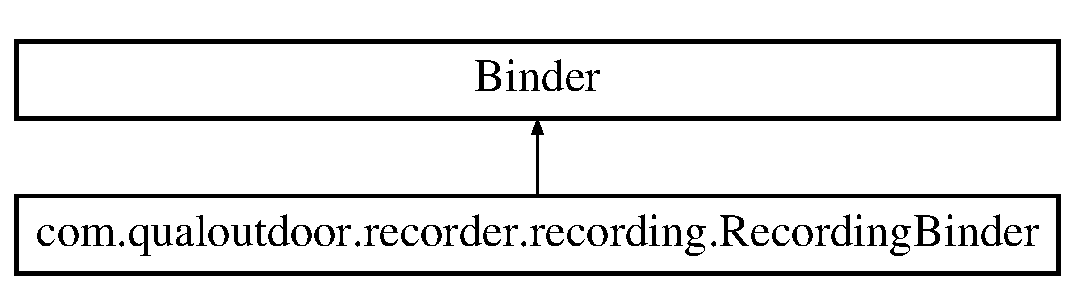
\includegraphics[height=2.000000cm]{classcom_1_1qualoutdoor_1_1recorder_1_1recording_1_1RecordingBinder}
\end{center}
\end{figure}
\subsection*{Public Member Functions}
\begin{DoxyCompactItemize}
\item 
\hyperlink{classcom_1_1qualoutdoor_1_1recorder_1_1recording_1_1RecordingBinder_a0d1cf5218f0acaff5461f1100f3b720d}{Recording\-Binder} (\hyperlink{classcom_1_1qualoutdoor_1_1recorder_1_1recording_1_1RecordingService}{Recording\-Service} service)
\item 
\hyperlink{classcom_1_1qualoutdoor_1_1recorder_1_1recording_1_1RecordingService}{Recording\-Service} \hyperlink{classcom_1_1qualoutdoor_1_1recorder_1_1recording_1_1RecordingBinder_aff514d1f17f94939e98fbdbcbe6f9426}{get\-Service} ()
\end{DoxyCompactItemize}
\subsection*{Private Attributes}
\begin{DoxyCompactItemize}
\item 
\hyperlink{classcom_1_1qualoutdoor_1_1recorder_1_1recording_1_1RecordingService}{Recording\-Service} \hyperlink{classcom_1_1qualoutdoor_1_1recorder_1_1recording_1_1RecordingBinder_a7db3901b1d36399d4f7f1c96ee328266}{my\-Service}
\end{DoxyCompactItemize}


\subsection{Detailed Description}
The local binder for the \hyperlink{classcom_1_1qualoutdoor_1_1recorder_1_1recording_1_1RecordingService}{Recording\-Service}. Caution, this works only if the service and the component binding to it are in the same process. 

Definition at line 9 of file Recording\-Binder.\-java.



\subsection{Constructor \& Destructor Documentation}
\hypertarget{classcom_1_1qualoutdoor_1_1recorder_1_1recording_1_1RecordingBinder_a0d1cf5218f0acaff5461f1100f3b720d}{\index{com\-::qualoutdoor\-::recorder\-::recording\-::\-Recording\-Binder@{com\-::qualoutdoor\-::recorder\-::recording\-::\-Recording\-Binder}!Recording\-Binder@{Recording\-Binder}}
\index{Recording\-Binder@{Recording\-Binder}!com::qualoutdoor::recorder::recording::RecordingBinder@{com\-::qualoutdoor\-::recorder\-::recording\-::\-Recording\-Binder}}
\subsubsection[{Recording\-Binder}]{\setlength{\rightskip}{0pt plus 5cm}com.\-qualoutdoor.\-recorder.\-recording.\-Recording\-Binder.\-Recording\-Binder (
\begin{DoxyParamCaption}
\item[{{\bf Recording\-Service}}]{service}
\end{DoxyParamCaption}
)}}\label{classcom_1_1qualoutdoor_1_1recorder_1_1recording_1_1RecordingBinder_a0d1cf5218f0acaff5461f1100f3b720d}
A constructor for the binder to know its service 

Definition at line 15 of file Recording\-Binder.\-java.



References com.\-qualoutdoor.\-recorder.\-recording.\-Recording\-Binder.\-my\-Service.



\subsection{Member Function Documentation}
\hypertarget{classcom_1_1qualoutdoor_1_1recorder_1_1recording_1_1RecordingBinder_aff514d1f17f94939e98fbdbcbe6f9426}{\index{com\-::qualoutdoor\-::recorder\-::recording\-::\-Recording\-Binder@{com\-::qualoutdoor\-::recorder\-::recording\-::\-Recording\-Binder}!get\-Service@{get\-Service}}
\index{get\-Service@{get\-Service}!com::qualoutdoor::recorder::recording::RecordingBinder@{com\-::qualoutdoor\-::recorder\-::recording\-::\-Recording\-Binder}}
\subsubsection[{get\-Service}]{\setlength{\rightskip}{0pt plus 5cm}{\bf Recording\-Service} com.\-qualoutdoor.\-recorder.\-recording.\-Recording\-Binder.\-get\-Service (
\begin{DoxyParamCaption}
{}
\end{DoxyParamCaption}
)}}\label{classcom_1_1qualoutdoor_1_1recorder_1_1recording_1_1RecordingBinder_aff514d1f17f94939e98fbdbcbe6f9426}
Get the service that provided this binder 

Definition at line 21 of file Recording\-Binder.\-java.



References com.\-qualoutdoor.\-recorder.\-recording.\-Recording\-Binder.\-my\-Service.



\subsection{Member Data Documentation}
\hypertarget{classcom_1_1qualoutdoor_1_1recorder_1_1recording_1_1RecordingBinder_a7db3901b1d36399d4f7f1c96ee328266}{\index{com\-::qualoutdoor\-::recorder\-::recording\-::\-Recording\-Binder@{com\-::qualoutdoor\-::recorder\-::recording\-::\-Recording\-Binder}!my\-Service@{my\-Service}}
\index{my\-Service@{my\-Service}!com::qualoutdoor::recorder::recording::RecordingBinder@{com\-::qualoutdoor\-::recorder\-::recording\-::\-Recording\-Binder}}
\subsubsection[{my\-Service}]{\setlength{\rightskip}{0pt plus 5cm}{\bf Recording\-Service} com.\-qualoutdoor.\-recorder.\-recording.\-Recording\-Binder.\-my\-Service\hspace{0.3cm}{\ttfamily [private]}}}\label{classcom_1_1qualoutdoor_1_1recorder_1_1recording_1_1RecordingBinder_a7db3901b1d36399d4f7f1c96ee328266}
The service that provided this binder 

Definition at line 12 of file Recording\-Binder.\-java.



Referenced by com.\-qualoutdoor.\-recorder.\-recording.\-Recording\-Binder.\-get\-Service(), and com.\-qualoutdoor.\-recorder.\-recording.\-Recording\-Binder.\-Recording\-Binder().



The documentation for this class was generated from the following file\-:\begin{DoxyCompactItemize}
\item 
src/com/qualoutdoor/recorder/recording/Recording\-Binder.\-java\end{DoxyCompactItemize}

\hypertarget{classcom_1_1qualoutdoor_1_1recorder_1_1recording_1_1RecordingService}{\section{com.\-qualoutdoor.\-recorder.\-recording.\-Recording\-Service Class Reference}
\label{classcom_1_1qualoutdoor_1_1recorder_1_1recording_1_1RecordingService}\index{com.\-qualoutdoor.\-recorder.\-recording.\-Recording\-Service@{com.\-qualoutdoor.\-recorder.\-recording.\-Recording\-Service}}
}
Inheritance diagram for com.\-qualoutdoor.\-recorder.\-recording.\-Recording\-Service\-:\begin{figure}[H]
\begin{center}
\leavevmode
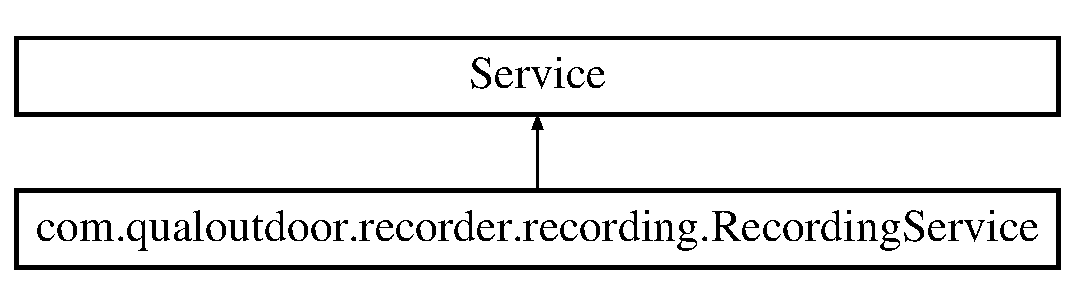
\includegraphics[height=2.000000cm]{classcom_1_1qualoutdoor_1_1recorder_1_1recording_1_1RecordingService}
\end{center}
\end{figure}
\subsection*{Public Member Functions}
\begin{DoxyCompactItemize}
\item 
\hypertarget{classcom_1_1qualoutdoor_1_1recorder_1_1recording_1_1RecordingService_a2e48946d240d2e6fcc41d4046b618321}{void {\bfseries on\-Create} ()}\label{classcom_1_1qualoutdoor_1_1recorder_1_1recording_1_1RecordingService_a2e48946d240d2e6fcc41d4046b618321}

\item 
\hypertarget{classcom_1_1qualoutdoor_1_1recorder_1_1recording_1_1RecordingService_a7ab6dab80edc8e3ad2b5a7436534d7f6}{I\-Binder {\bfseries on\-Bind} (Intent intent)}\label{classcom_1_1qualoutdoor_1_1recorder_1_1recording_1_1RecordingService_a7ab6dab80edc8e3ad2b5a7436534d7f6}

\item 
boolean \hyperlink{classcom_1_1qualoutdoor_1_1recorder_1_1recording_1_1RecordingService_a97c5a5525e4f024ed981f8a4167c0c8f}{is\-Recording} ()
\item 
void \hyperlink{classcom_1_1qualoutdoor_1_1recorder_1_1recording_1_1RecordingService_a7a2a7a176fba147bbc3eb753aa819513}{set\-Sampling\-Rate} (int millis)
\item 
\hypertarget{classcom_1_1qualoutdoor_1_1recorder_1_1recording_1_1RecordingService_a9614d87abfd09a76f082d5c37cf06de2}{int {\bfseries on\-Start\-Command} (Intent intent, int flags, int start\-Id)}\label{classcom_1_1qualoutdoor_1_1recorder_1_1recording_1_1RecordingService_a9614d87abfd09a76f082d5c37cf06de2}

\item 
\hypertarget{classcom_1_1qualoutdoor_1_1recorder_1_1recording_1_1RecordingService_ad97856ad8728cbbc102e664b934982bc}{void {\bfseries on\-Destroy} ()}\label{classcom_1_1qualoutdoor_1_1recorder_1_1recording_1_1RecordingService_ad97856ad8728cbbc102e664b934982bc}

\item 
void \hyperlink{classcom_1_1qualoutdoor_1_1recorder_1_1recording_1_1RecordingService_a51bcaacd57cecbbc192ae10ee0548898}{stop\-Recording} ()
\end{DoxyCompactItemize}
\subsection*{Private Member Functions}
\begin{DoxyCompactItemize}
\item 
void \hyperlink{classcom_1_1qualoutdoor_1_1recorder_1_1recording_1_1RecordingService_ad1e000af998ea34d8cd646c73b38f12a}{start\-Recording} ()
\end{DoxyCompactItemize}
\subsection*{Private Attributes}
\begin{DoxyCompactItemize}
\item 
I\-Binder \hyperlink{classcom_1_1qualoutdoor_1_1recorder_1_1recording_1_1RecordingService_ac19023b61b61f80ce69723f5ac3e78f7}{m\-Recording\-Binder}
\item 
boolean \hyperlink{classcom_1_1qualoutdoor_1_1recorder_1_1recording_1_1RecordingService_aa44bc8a3d8265952f589faa7ce35d3d4}{is\-Recording} = false
\item 
Thread \hyperlink{classcom_1_1qualoutdoor_1_1recorder_1_1recording_1_1RecordingService_a17aeabbe9a9d27439c297bbf1ff4d3eb}{thread}
\end{DoxyCompactItemize}


\subsection{Detailed Description}
This service when started will link to the Telephony\-Service and begin sampling the phone state. One can bind to this service in order to modify the sampling rate. It is needed to call stop\-Service() on it in order to stop the recording process. 

Definition at line 17 of file Recording\-Service.\-java.



\subsection{Member Function Documentation}
\hypertarget{classcom_1_1qualoutdoor_1_1recorder_1_1recording_1_1RecordingService_a97c5a5525e4f024ed981f8a4167c0c8f}{\index{com\-::qualoutdoor\-::recorder\-::recording\-::\-Recording\-Service@{com\-::qualoutdoor\-::recorder\-::recording\-::\-Recording\-Service}!is\-Recording@{is\-Recording}}
\index{is\-Recording@{is\-Recording}!com::qualoutdoor::recorder::recording::RecordingService@{com\-::qualoutdoor\-::recorder\-::recording\-::\-Recording\-Service}}
\subsubsection[{is\-Recording}]{\setlength{\rightskip}{0pt plus 5cm}boolean com.\-qualoutdoor.\-recorder.\-recording.\-Recording\-Service.\-is\-Recording (
\begin{DoxyParamCaption}
{}
\end{DoxyParamCaption}
)}}\label{classcom_1_1qualoutdoor_1_1recorder_1_1recording_1_1RecordingService_a97c5a5525e4f024ed981f8a4167c0c8f}
Indicates whether the service is currently recording data 

Definition at line 44 of file Recording\-Service.\-java.



Referenced by com.\-qualoutdoor.\-recorder.\-recording.\-Recording\-Service.\-start\-Recording(), and com.\-qualoutdoor.\-recorder.\-recording.\-Recording\-Service.\-stop\-Recording().

\hypertarget{classcom_1_1qualoutdoor_1_1recorder_1_1recording_1_1RecordingService_a7a2a7a176fba147bbc3eb753aa819513}{\index{com\-::qualoutdoor\-::recorder\-::recording\-::\-Recording\-Service@{com\-::qualoutdoor\-::recorder\-::recording\-::\-Recording\-Service}!set\-Sampling\-Rate@{set\-Sampling\-Rate}}
\index{set\-Sampling\-Rate@{set\-Sampling\-Rate}!com::qualoutdoor::recorder::recording::RecordingService@{com\-::qualoutdoor\-::recorder\-::recording\-::\-Recording\-Service}}
\subsubsection[{set\-Sampling\-Rate}]{\setlength{\rightskip}{0pt plus 5cm}void com.\-qualoutdoor.\-recorder.\-recording.\-Recording\-Service.\-set\-Sampling\-Rate (
\begin{DoxyParamCaption}
\item[{int}]{millis}
\end{DoxyParamCaption}
)}}\label{classcom_1_1qualoutdoor_1_1recorder_1_1recording_1_1RecordingService_a7a2a7a176fba147bbc3eb753aa819513}
Set the sampling rate to the specified value in milliseconds 

Definition at line 49 of file Recording\-Service.\-java.

\hypertarget{classcom_1_1qualoutdoor_1_1recorder_1_1recording_1_1RecordingService_ad1e000af998ea34d8cd646c73b38f12a}{\index{com\-::qualoutdoor\-::recorder\-::recording\-::\-Recording\-Service@{com\-::qualoutdoor\-::recorder\-::recording\-::\-Recording\-Service}!start\-Recording@{start\-Recording}}
\index{start\-Recording@{start\-Recording}!com::qualoutdoor::recorder::recording::RecordingService@{com\-::qualoutdoor\-::recorder\-::recording\-::\-Recording\-Service}}
\subsubsection[{start\-Recording}]{\setlength{\rightskip}{0pt plus 5cm}void com.\-qualoutdoor.\-recorder.\-recording.\-Recording\-Service.\-start\-Recording (
\begin{DoxyParamCaption}
{}
\end{DoxyParamCaption}
)\hspace{0.3cm}{\ttfamily [private]}}}\label{classcom_1_1qualoutdoor_1_1recorder_1_1recording_1_1RecordingService_ad1e000af998ea34d8cd646c73b38f12a}
Start the recording process. 

Definition at line 73 of file Recording\-Service.\-java.



References com.\-qualoutdoor.\-recorder.\-notifications.\-Notification\-Center.\-B\-A\-C\-K\-G\-R\-O\-U\-N\-D\-\_\-\-R\-E\-C\-O\-R\-D\-I\-N\-G, com.\-qualoutdoor.\-recorder.\-recording.\-Recording\-Service.\-is\-Recording(), and com.\-qualoutdoor.\-recorder.\-recording.\-Recording\-Service.\-thread.

\hypertarget{classcom_1_1qualoutdoor_1_1recorder_1_1recording_1_1RecordingService_a51bcaacd57cecbbc192ae10ee0548898}{\index{com\-::qualoutdoor\-::recorder\-::recording\-::\-Recording\-Service@{com\-::qualoutdoor\-::recorder\-::recording\-::\-Recording\-Service}!stop\-Recording@{stop\-Recording}}
\index{stop\-Recording@{stop\-Recording}!com::qualoutdoor::recorder::recording::RecordingService@{com\-::qualoutdoor\-::recorder\-::recording\-::\-Recording\-Service}}
\subsubsection[{stop\-Recording}]{\setlength{\rightskip}{0pt plus 5cm}void com.\-qualoutdoor.\-recorder.\-recording.\-Recording\-Service.\-stop\-Recording (
\begin{DoxyParamCaption}
{}
\end{DoxyParamCaption}
)}}\label{classcom_1_1qualoutdoor_1_1recorder_1_1recording_1_1RecordingService_a51bcaacd57cecbbc192ae10ee0548898}
Stop the recording process 

Definition at line 102 of file Recording\-Service.\-java.



References com.\-qualoutdoor.\-recorder.\-recording.\-Recording\-Service.\-is\-Recording(), and com.\-qualoutdoor.\-recorder.\-recording.\-Recording\-Service.\-thread.



\subsection{Member Data Documentation}
\hypertarget{classcom_1_1qualoutdoor_1_1recorder_1_1recording_1_1RecordingService_aa44bc8a3d8265952f589faa7ce35d3d4}{\index{com\-::qualoutdoor\-::recorder\-::recording\-::\-Recording\-Service@{com\-::qualoutdoor\-::recorder\-::recording\-::\-Recording\-Service}!is\-Recording@{is\-Recording}}
\index{is\-Recording@{is\-Recording}!com::qualoutdoor::recorder::recording::RecordingService@{com\-::qualoutdoor\-::recorder\-::recording\-::\-Recording\-Service}}
\subsubsection[{is\-Recording}]{\setlength{\rightskip}{0pt plus 5cm}boolean com.\-qualoutdoor.\-recorder.\-recording.\-Recording\-Service.\-is\-Recording = false\hspace{0.3cm}{\ttfamily [private]}}}\label{classcom_1_1qualoutdoor_1_1recorder_1_1recording_1_1RecordingService_aa44bc8a3d8265952f589faa7ce35d3d4}
Indicates if a recording process is ongoing 

Definition at line 22 of file Recording\-Service.\-java.

\hypertarget{classcom_1_1qualoutdoor_1_1recorder_1_1recording_1_1RecordingService_ac19023b61b61f80ce69723f5ac3e78f7}{\index{com\-::qualoutdoor\-::recorder\-::recording\-::\-Recording\-Service@{com\-::qualoutdoor\-::recorder\-::recording\-::\-Recording\-Service}!m\-Recording\-Binder@{m\-Recording\-Binder}}
\index{m\-Recording\-Binder@{m\-Recording\-Binder}!com::qualoutdoor::recorder::recording::RecordingService@{com\-::qualoutdoor\-::recorder\-::recording\-::\-Recording\-Service}}
\subsubsection[{m\-Recording\-Binder}]{\setlength{\rightskip}{0pt plus 5cm}I\-Binder com.\-qualoutdoor.\-recorder.\-recording.\-Recording\-Service.\-m\-Recording\-Binder\hspace{0.3cm}{\ttfamily [private]}}}\label{classcom_1_1qualoutdoor_1_1recorder_1_1recording_1_1RecordingService_ac19023b61b61f80ce69723f5ac3e78f7}
The interface binder for this service 

Definition at line 20 of file Recording\-Service.\-java.

\hypertarget{classcom_1_1qualoutdoor_1_1recorder_1_1recording_1_1RecordingService_a17aeabbe9a9d27439c297bbf1ff4d3eb}{\index{com\-::qualoutdoor\-::recorder\-::recording\-::\-Recording\-Service@{com\-::qualoutdoor\-::recorder\-::recording\-::\-Recording\-Service}!thread@{thread}}
\index{thread@{thread}!com::qualoutdoor::recorder::recording::RecordingService@{com\-::qualoutdoor\-::recorder\-::recording\-::\-Recording\-Service}}
\subsubsection[{thread}]{\setlength{\rightskip}{0pt plus 5cm}Thread com.\-qualoutdoor.\-recorder.\-recording.\-Recording\-Service.\-thread\hspace{0.3cm}{\ttfamily [private]}}}\label{classcom_1_1qualoutdoor_1_1recorder_1_1recording_1_1RecordingService_a17aeabbe9a9d27439c297bbf1ff4d3eb}
A fake recording thread 

Definition at line 25 of file Recording\-Service.\-java.



Referenced by com.\-qualoutdoor.\-recorder.\-recording.\-Recording\-Service.\-start\-Recording(), and com.\-qualoutdoor.\-recorder.\-recording.\-Recording\-Service.\-stop\-Recording().



The documentation for this class was generated from the following file\-:\begin{DoxyCompactItemize}
\item 
src/com/qualoutdoor/recorder/recording/Recording\-Service.\-java\end{DoxyCompactItemize}

\hypertarget{classcom_1_1qualoutdoor_1_1recorder_1_1recording_1_1RecordingServiceConnection}{\section{com.\-qualoutdoor.\-recorder.\-recording.\-Recording\-Service\-Connection Class Reference}
\label{classcom_1_1qualoutdoor_1_1recorder_1_1recording_1_1RecordingServiceConnection}\index{com.\-qualoutdoor.\-recorder.\-recording.\-Recording\-Service\-Connection@{com.\-qualoutdoor.\-recorder.\-recording.\-Recording\-Service\-Connection}}
}
Inheritance diagram for com.\-qualoutdoor.\-recorder.\-recording.\-Recording\-Service\-Connection\-:\begin{figure}[H]
\begin{center}
\leavevmode
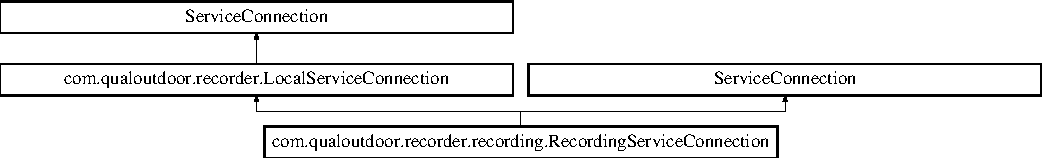
\includegraphics[height=2.121212cm]{classcom_1_1qualoutdoor_1_1recorder_1_1recording_1_1RecordingServiceConnection}
\end{center}
\end{figure}
\subsection*{Public Member Functions}
\begin{DoxyCompactItemize}
\item 
\hypertarget{classcom_1_1qualoutdoor_1_1recorder_1_1recording_1_1RecordingServiceConnection_a150438c50b77f52c96951846a65f0748}{void {\bfseries on\-Service\-Connected} (Component\-Name service\-Name, I\-Binder binder)}\label{classcom_1_1qualoutdoor_1_1recorder_1_1recording_1_1RecordingServiceConnection_a150438c50b77f52c96951846a65f0748}

\item 
\hyperlink{classcom_1_1qualoutdoor_1_1recorder_1_1recording_1_1RecordingService}{Recording\-Service} \hyperlink{classcom_1_1qualoutdoor_1_1recorder_1_1recording_1_1RecordingServiceConnection_a10e61e4e5c92174b21264df6c3a1247b}{get\-Service} ()
\end{DoxyCompactItemize}
\subsection*{Private Attributes}
\begin{DoxyCompactItemize}
\item 
\hyperlink{classcom_1_1qualoutdoor_1_1recorder_1_1recording_1_1RecordingService}{Recording\-Service} \hyperlink{classcom_1_1qualoutdoor_1_1recorder_1_1recording_1_1RecordingServiceConnection_a8eb8ebee30e9b3f9264935bc7277ae5e}{service}
\end{DoxyCompactItemize}
\subsection*{Additional Inherited Members}


\subsection{Detailed Description}
An implementation for a local Service\-Connection to the \hyperlink{classcom_1_1qualoutdoor_1_1recorder_1_1recording_1_1RecordingService}{Recording\-Service}. Caution \-: this necessitate the binder to be cast into \hyperlink{classcom_1_1qualoutdoor_1_1recorder_1_1recording_1_1RecordingBinder}{Recording\-Binder} on connection. This works because our services belong to the same process. 

Definition at line 15 of file Recording\-Service\-Connection.\-java.



\subsection{Member Function Documentation}
\hypertarget{classcom_1_1qualoutdoor_1_1recorder_1_1recording_1_1RecordingServiceConnection_a10e61e4e5c92174b21264df6c3a1247b}{\index{com\-::qualoutdoor\-::recorder\-::recording\-::\-Recording\-Service\-Connection@{com\-::qualoutdoor\-::recorder\-::recording\-::\-Recording\-Service\-Connection}!get\-Service@{get\-Service}}
\index{get\-Service@{get\-Service}!com::qualoutdoor::recorder::recording::RecordingServiceConnection@{com\-::qualoutdoor\-::recorder\-::recording\-::\-Recording\-Service\-Connection}}
\subsubsection[{get\-Service}]{\setlength{\rightskip}{0pt plus 5cm}{\bf Recording\-Service} com.\-qualoutdoor.\-recorder.\-recording.\-Recording\-Service\-Connection.\-get\-Service (
\begin{DoxyParamCaption}
{}
\end{DoxyParamCaption}
)}}\label{classcom_1_1qualoutdoor_1_1recorder_1_1recording_1_1RecordingServiceConnection_a10e61e4e5c92174b21264df6c3a1247b}
Get the binder 

Definition at line 34 of file Recording\-Service\-Connection.\-java.



References com.\-qualoutdoor.\-recorder.\-recording.\-Recording\-Service\-Connection.\-service.



\subsection{Member Data Documentation}
\hypertarget{classcom_1_1qualoutdoor_1_1recorder_1_1recording_1_1RecordingServiceConnection_a8eb8ebee30e9b3f9264935bc7277ae5e}{\index{com\-::qualoutdoor\-::recorder\-::recording\-::\-Recording\-Service\-Connection@{com\-::qualoutdoor\-::recorder\-::recording\-::\-Recording\-Service\-Connection}!service@{service}}
\index{service@{service}!com::qualoutdoor::recorder::recording::RecordingServiceConnection@{com\-::qualoutdoor\-::recorder\-::recording\-::\-Recording\-Service\-Connection}}
\subsubsection[{service}]{\setlength{\rightskip}{0pt plus 5cm}{\bf Recording\-Service} com.\-qualoutdoor.\-recorder.\-recording.\-Recording\-Service\-Connection.\-service\hspace{0.3cm}{\ttfamily [private]}}}\label{classcom_1_1qualoutdoor_1_1recorder_1_1recording_1_1RecordingServiceConnection_a8eb8ebee30e9b3f9264935bc7277ae5e}
The recording service we connected to 

Definition at line 19 of file Recording\-Service\-Connection.\-java.



Referenced by com.\-qualoutdoor.\-recorder.\-recording.\-Recording\-Service\-Connection.\-get\-Service().



The documentation for this class was generated from the following file\-:\begin{DoxyCompactItemize}
\item 
src/com/qualoutdoor/recorder/recording/Recording\-Service\-Connection.\-java\end{DoxyCompactItemize}

\hypertarget{classcom_1_1qualoutdoor_1_1recorder_1_1SamplingButton}{\section{com.\-qualoutdoor.\-recorder.\-Sampling\-Button Class Reference}
\label{classcom_1_1qualoutdoor_1_1recorder_1_1SamplingButton}\index{com.\-qualoutdoor.\-recorder.\-Sampling\-Button@{com.\-qualoutdoor.\-recorder.\-Sampling\-Button}}
}
Inheritance diagram for com.\-qualoutdoor.\-recorder.\-Sampling\-Button\-:\begin{figure}[H]
\begin{center}
\leavevmode
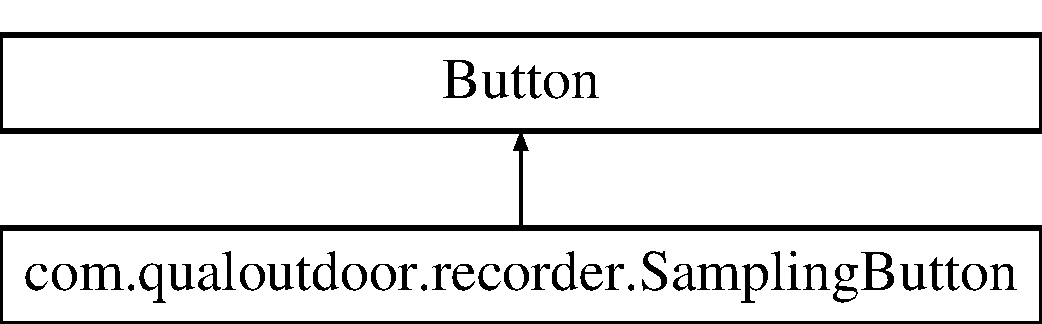
\includegraphics[height=2.000000cm]{classcom_1_1qualoutdoor_1_1recorder_1_1SamplingButton}
\end{center}
\end{figure}
\subsection*{Public Member Functions}
\begin{DoxyCompactItemize}
\item 
\hypertarget{classcom_1_1qualoutdoor_1_1recorder_1_1SamplingButton_a55589a649bdfe2239dfd393b881ce54f}{{\bfseries Sampling\-Button} (Context context)}\label{classcom_1_1qualoutdoor_1_1recorder_1_1SamplingButton_a55589a649bdfe2239dfd393b881ce54f}

\item 
\hypertarget{classcom_1_1qualoutdoor_1_1recorder_1_1SamplingButton_a8b79ac727cf80e71c7645e04c85b43cd}{{\bfseries Sampling\-Button} (Context context, Attribute\-Set attrs, int def\-Style)}\label{classcom_1_1qualoutdoor_1_1recorder_1_1SamplingButton_a8b79ac727cf80e71c7645e04c85b43cd}

\item 
\hypertarget{classcom_1_1qualoutdoor_1_1recorder_1_1SamplingButton_a4b2541d9897473bd79bcc5f5549971d7}{{\bfseries Sampling\-Button} (Context context, Attribute\-Set attrs)}\label{classcom_1_1qualoutdoor_1_1recorder_1_1SamplingButton_a4b2541d9897473bd79bcc5f5549971d7}

\end{DoxyCompactItemize}
\subsection*{Protected Member Functions}
\begin{DoxyCompactItemize}
\item 
\hypertarget{classcom_1_1qualoutdoor_1_1recorder_1_1SamplingButton_a087dee4090dc9aba9ef58b6a419ea128}{void {\bfseries on\-Attached\-To\-Window} ()}\label{classcom_1_1qualoutdoor_1_1recorder_1_1SamplingButton_a087dee4090dc9aba9ef58b6a419ea128}

\end{DoxyCompactItemize}
\subsection*{Private Member Functions}
\begin{DoxyCompactItemize}
\item 
\hypertarget{classcom_1_1qualoutdoor_1_1recorder_1_1SamplingButton_a7ef3a0d5d2622d8597285e4812e19e22}{void {\bfseries action\-Start\-Stop} (View view)}\label{classcom_1_1qualoutdoor_1_1recorder_1_1SamplingButton_a7ef3a0d5d2622d8597285e4812e19e22}

\end{DoxyCompactItemize}


\subsection{Detailed Description}
A button which starts or stops the background sampling (this only displays notification) 

Definition at line 12 of file Sampling\-Button.\-java.



The documentation for this class was generated from the following file\-:\begin{DoxyCompactItemize}
\item 
src/com/qualoutdoor/recorder/Sampling\-Button.\-java\end{DoxyCompactItemize}

\hypertarget{classcom_1_1qualoutdoor_1_1recorder_1_1scripts_1_1ScriptListFragment}{\section{com.\-qualoutdoor.\-recorder.\-scripts.\-Script\-List\-Fragment Class Reference}
\label{classcom_1_1qualoutdoor_1_1recorder_1_1scripts_1_1ScriptListFragment}\index{com.\-qualoutdoor.\-recorder.\-scripts.\-Script\-List\-Fragment@{com.\-qualoutdoor.\-recorder.\-scripts.\-Script\-List\-Fragment}}
}
Inheritance diagram for com.\-qualoutdoor.\-recorder.\-scripts.\-Script\-List\-Fragment\-:\begin{figure}[H]
\begin{center}
\leavevmode
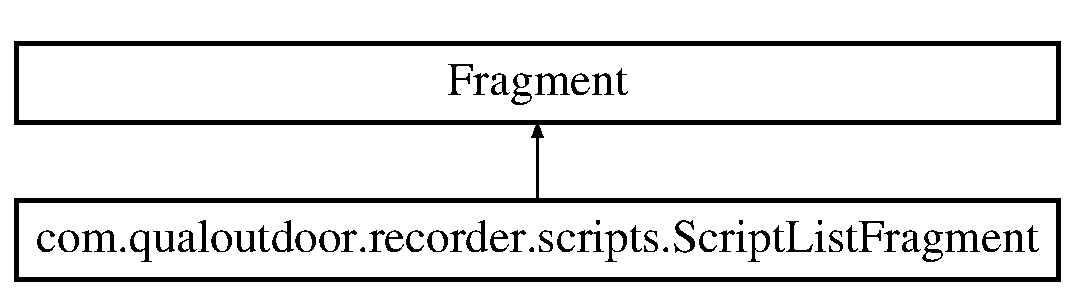
\includegraphics[height=2.000000cm]{classcom_1_1qualoutdoor_1_1recorder_1_1scripts_1_1ScriptListFragment}
\end{center}
\end{figure}
\subsection*{Public Member Functions}
\begin{DoxyCompactItemize}
\item 
\hypertarget{classcom_1_1qualoutdoor_1_1recorder_1_1scripts_1_1ScriptListFragment_adf19ceaee6c2ccc3395ba471f37ea24f}{View {\bfseries on\-Create\-View} (Layout\-Inflater inflater, View\-Group container, Bundle saved\-Instance\-State)}\label{classcom_1_1qualoutdoor_1_1recorder_1_1scripts_1_1ScriptListFragment_adf19ceaee6c2ccc3395ba471f37ea24f}

\end{DoxyCompactItemize}


\subsection{Detailed Description}


Definition at line 11 of file Script\-List\-Fragment.\-java.



The documentation for this class was generated from the following file\-:\begin{DoxyCompactItemize}
\item 
src/com/qualoutdoor/recorder/scripts/Script\-List\-Fragment.\-java\end{DoxyCompactItemize}

\hypertarget{classcom_1_1qualoutdoor_1_1recorder_1_1settings_1_1SettingsActivity}{\section{com.\-qualoutdoor.\-recorder.\-settings.\-Settings\-Activity Class Reference}
\label{classcom_1_1qualoutdoor_1_1recorder_1_1settings_1_1SettingsActivity}\index{com.\-qualoutdoor.\-recorder.\-settings.\-Settings\-Activity@{com.\-qualoutdoor.\-recorder.\-settings.\-Settings\-Activity}}
}
Inheritance diagram for com.\-qualoutdoor.\-recorder.\-settings.\-Settings\-Activity\-:\begin{figure}[H]
\begin{center}
\leavevmode
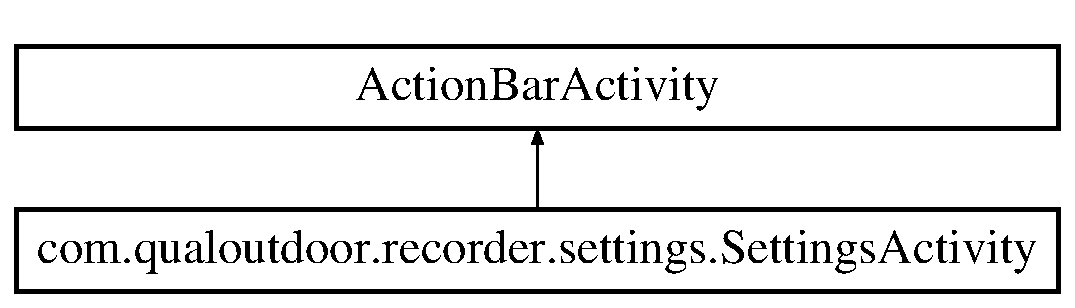
\includegraphics[height=2.000000cm]{classcom_1_1qualoutdoor_1_1recorder_1_1settings_1_1SettingsActivity}
\end{center}
\end{figure}
\subsection*{Protected Member Functions}
\begin{DoxyCompactItemize}
\item 
\hypertarget{classcom_1_1qualoutdoor_1_1recorder_1_1settings_1_1SettingsActivity_af9a3a25e675b25b179091becbd9c3a28}{void {\bfseries on\-Create} (Bundle saved\-Instance\-State)}\label{classcom_1_1qualoutdoor_1_1recorder_1_1settings_1_1SettingsActivity_af9a3a25e675b25b179091becbd9c3a28}

\end{DoxyCompactItemize}


\subsection{Detailed Description}


Definition at line 8 of file Settings\-Activity.\-java.



The documentation for this class was generated from the following file\-:\begin{DoxyCompactItemize}
\item 
src/com/qualoutdoor/recorder/settings/Settings\-Activity.\-java\end{DoxyCompactItemize}

\hypertarget{classcom_1_1qualoutdoor_1_1recorder_1_1charting_1_1SignalStrengthPlotFragment}{\section{com.\-qualoutdoor.\-recorder.\-charting.\-Signal\-Strength\-Plot\-Fragment Class Reference}
\label{classcom_1_1qualoutdoor_1_1recorder_1_1charting_1_1SignalStrengthPlotFragment}\index{com.\-qualoutdoor.\-recorder.\-charting.\-Signal\-Strength\-Plot\-Fragment@{com.\-qualoutdoor.\-recorder.\-charting.\-Signal\-Strength\-Plot\-Fragment}}
}
Inheritance diagram for com.\-qualoutdoor.\-recorder.\-charting.\-Signal\-Strength\-Plot\-Fragment\-:\begin{figure}[H]
\begin{center}
\leavevmode
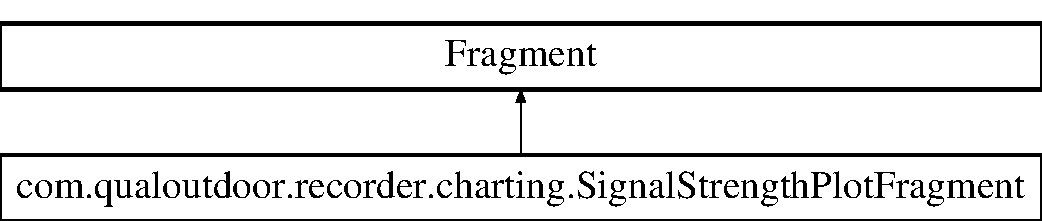
\includegraphics[height=2.000000cm]{classcom_1_1qualoutdoor_1_1recorder_1_1charting_1_1SignalStrengthPlotFragment}
\end{center}
\end{figure}
\subsection*{Classes}
\begin{DoxyCompactItemize}
\item 
class \hyperlink{classcom_1_1qualoutdoor_1_1recorder_1_1charting_1_1SignalStrengthPlotFragment_1_1MyPlotUpdater}{My\-Plot\-Updater}
\end{DoxyCompactItemize}
\subsection*{Public Member Functions}
\begin{DoxyCompactItemize}
\item 
\hypertarget{classcom_1_1qualoutdoor_1_1recorder_1_1charting_1_1SignalStrengthPlotFragment_a6ae8c5a953179150a5fea9316a1357b1}{View {\bfseries on\-Create\-View} (Layout\-Inflater inflater, View\-Group container, Bundle saved\-Instance\-State)}\label{classcom_1_1qualoutdoor_1_1recorder_1_1charting_1_1SignalStrengthPlotFragment_a6ae8c5a953179150a5fea9316a1357b1}

\item 
\hypertarget{classcom_1_1qualoutdoor_1_1recorder_1_1charting_1_1SignalStrengthPlotFragment_aa4786952a20f614f230eebba2463ab5c}{void {\bfseries on\-Activity\-Created} (Bundle saved\-Instance\-State)}\label{classcom_1_1qualoutdoor_1_1recorder_1_1charting_1_1SignalStrengthPlotFragment_aa4786952a20f614f230eebba2463ab5c}

\item 
\hypertarget{classcom_1_1qualoutdoor_1_1recorder_1_1charting_1_1SignalStrengthPlotFragment_a1dc4240b9f2a8ddb6ba8bf5a1c4c9b21}{void {\bfseries on\-Destroy} ()}\label{classcom_1_1qualoutdoor_1_1recorder_1_1charting_1_1SignalStrengthPlotFragment_a1dc4240b9f2a8ddb6ba8bf5a1c4c9b21}

\end{DoxyCompactItemize}
\subsection*{Private Attributes}
\begin{DoxyCompactItemize}
\item 
\hypertarget{classcom_1_1qualoutdoor_1_1recorder_1_1charting_1_1SignalStrengthPlotFragment_ae8f6b6a16aacf738466b6bf749b58085}{Telephony\-Manager {\bfseries telephony\-Manager}}\label{classcom_1_1qualoutdoor_1_1recorder_1_1charting_1_1SignalStrengthPlotFragment_ae8f6b6a16aacf738466b6bf749b58085}

\item 
\hypertarget{classcom_1_1qualoutdoor_1_1recorder_1_1charting_1_1SignalStrengthPlotFragment_ad4c2fb48286d47b1d96c0092b6938c24}{\hyperlink{classcom_1_1qualoutdoor_1_1recorder_1_1charting_1_1SignalStrengthSampler}{Signal\-Strength\-Sampler} {\bfseries ss\-Sampler}}\label{classcom_1_1qualoutdoor_1_1recorder_1_1charting_1_1SignalStrengthPlotFragment_ad4c2fb48286d47b1d96c0092b6938c24}

\item 
\hypertarget{classcom_1_1qualoutdoor_1_1recorder_1_1charting_1_1SignalStrengthPlotFragment_a5fc7e28e4085e975aa3ab8e3ff180285}{Thread {\bfseries thread}}\label{classcom_1_1qualoutdoor_1_1recorder_1_1charting_1_1SignalStrengthPlotFragment_a5fc7e28e4085e975aa3ab8e3ff180285}

\item 
\hypertarget{classcom_1_1qualoutdoor_1_1recorder_1_1charting_1_1SignalStrengthPlotFragment_af5f66cd050b8c3f9a9eca32c1c9ce717}{X\-Y\-Plot {\bfseries dynamic\-Plot}}\label{classcom_1_1qualoutdoor_1_1recorder_1_1charting_1_1SignalStrengthPlotFragment_af5f66cd050b8c3f9a9eca32c1c9ce717}

\item 
\hypertarget{classcom_1_1qualoutdoor_1_1recorder_1_1charting_1_1SignalStrengthPlotFragment_a4a7d083f0421d83ea983d0e1baef3516}{\hyperlink{classcom_1_1qualoutdoor_1_1recorder_1_1charting_1_1SignalStrengthPlotFragment_1_1MyPlotUpdater}{My\-Plot\-Updater} {\bfseries plot\-Updater}}\label{classcom_1_1qualoutdoor_1_1recorder_1_1charting_1_1SignalStrengthPlotFragment_a4a7d083f0421d83ea983d0e1baef3516}

\item 
\hypertarget{classcom_1_1qualoutdoor_1_1recorder_1_1charting_1_1SignalStrengthPlotFragment_a8343d4d21238d54faf1759c65290b813}{Simple\-X\-Y\-Series {\bfseries ss\-Lvl\-Series}}\label{classcom_1_1qualoutdoor_1_1recorder_1_1charting_1_1SignalStrengthPlotFragment_a8343d4d21238d54faf1759c65290b813}

\end{DoxyCompactItemize}
\subsection*{Static Private Attributes}
\begin{DoxyCompactItemize}
\item 
\hypertarget{classcom_1_1qualoutdoor_1_1recorder_1_1charting_1_1SignalStrengthPlotFragment_aa6d119ce9035b9702eb896eca26e2c21}{static final int {\bfseries S\-A\-M\-P\-L\-E\-\_\-\-R\-A\-T\-E} = 1000}\label{classcom_1_1qualoutdoor_1_1recorder_1_1charting_1_1SignalStrengthPlotFragment_aa6d119ce9035b9702eb896eca26e2c21}

\item 
\hypertarget{classcom_1_1qualoutdoor_1_1recorder_1_1charting_1_1SignalStrengthPlotFragment_a5221a8dba9576dce9067909e4b7da1bb}{static final int {\bfseries H\-I\-S\-T\-O\-R\-Y\-\_\-\-S\-I\-Z\-E} = 60}\label{classcom_1_1qualoutdoor_1_1recorder_1_1charting_1_1SignalStrengthPlotFragment_a5221a8dba9576dce9067909e4b7da1bb}

\item 
\hypertarget{classcom_1_1qualoutdoor_1_1recorder_1_1charting_1_1SignalStrengthPlotFragment_ad09ee6d037a562b4fcbe7971e8f4c7a8}{static final int {\bfseries M\-I\-N\-\_\-\-S\-S} = -\/113}\label{classcom_1_1qualoutdoor_1_1recorder_1_1charting_1_1SignalStrengthPlotFragment_ad09ee6d037a562b4fcbe7971e8f4c7a8}

\item 
\hypertarget{classcom_1_1qualoutdoor_1_1recorder_1_1charting_1_1SignalStrengthPlotFragment_a5488d5038578b49d6ec52ee159dbcf30}{static final int {\bfseries M\-A\-X\-\_\-\-S\-S} = -\/60}\label{classcom_1_1qualoutdoor_1_1recorder_1_1charting_1_1SignalStrengthPlotFragment_a5488d5038578b49d6ec52ee159dbcf30}

\end{DoxyCompactItemize}


\subsection{Detailed Description}


Definition at line 25 of file Signal\-Strength\-Plot\-Fragment.\-java.



The documentation for this class was generated from the following file\-:\begin{DoxyCompactItemize}
\item 
src/com/qualoutdoor/recorder/charting/Signal\-Strength\-Plot\-Fragment.\-java\end{DoxyCompactItemize}

\hypertarget{classcom_1_1qualoutdoor_1_1recorder_1_1charting_1_1SignalStrengthSampler}{\section{com.\-qualoutdoor.\-recorder.\-charting.\-Signal\-Strength\-Sampler Class Reference}
\label{classcom_1_1qualoutdoor_1_1recorder_1_1charting_1_1SignalStrengthSampler}\index{com.\-qualoutdoor.\-recorder.\-charting.\-Signal\-Strength\-Sampler@{com.\-qualoutdoor.\-recorder.\-charting.\-Signal\-Strength\-Sampler}}
}
Inheritance diagram for com.\-qualoutdoor.\-recorder.\-charting.\-Signal\-Strength\-Sampler\-:\begin{figure}[H]
\begin{center}
\leavevmode
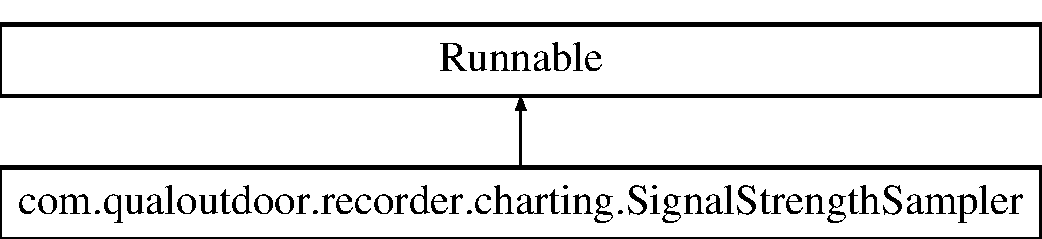
\includegraphics[height=2.000000cm]{classcom_1_1qualoutdoor_1_1recorder_1_1charting_1_1SignalStrengthSampler}
\end{center}
\end{figure}
\subsection*{Classes}
\begin{DoxyCompactItemize}
\item 
class {\bfseries My\-Observable}
\item 
class \hyperlink{classcom_1_1qualoutdoor_1_1recorder_1_1charting_1_1SignalStrengthSampler_1_1MyPhoneStateListener}{My\-Phone\-State\-Listener}
\end{DoxyCompactItemize}
\subsection*{Public Member Functions}
\begin{DoxyCompactItemize}
\item 
\hypertarget{classcom_1_1qualoutdoor_1_1recorder_1_1charting_1_1SignalStrengthSampler_a49109a8e7ef2a4d11e3065aa942e61a5}{{\bfseries Signal\-Strength\-Sampler} (int sampling\-Rate)}\label{classcom_1_1qualoutdoor_1_1recorder_1_1charting_1_1SignalStrengthSampler_a49109a8e7ef2a4d11e3065aa942e61a5}

\item 
\hypertarget{classcom_1_1qualoutdoor_1_1recorder_1_1charting_1_1SignalStrengthSampler_a05d2c5bcbcb8cb93b141407aff0c37e9}{void {\bfseries run} ()}\label{classcom_1_1qualoutdoor_1_1recorder_1_1charting_1_1SignalStrengthSampler_a05d2c5bcbcb8cb93b141407aff0c37e9}

\item 
\hypertarget{classcom_1_1qualoutdoor_1_1recorder_1_1charting_1_1SignalStrengthSampler_a21694fad264b9b83b7e356d6886c80a0}{synchronized Signal\-Strength {\bfseries get\-Signal\-Strength} ()}\label{classcom_1_1qualoutdoor_1_1recorder_1_1charting_1_1SignalStrengthSampler_a21694fad264b9b83b7e356d6886c80a0}

\item 
\hypertarget{classcom_1_1qualoutdoor_1_1recorder_1_1charting_1_1SignalStrengthSampler_ab3fea61441f89a891403fcd431059d1c}{Phone\-State\-Listener {\bfseries get\-Phone\-State\-Listener} ()}\label{classcom_1_1qualoutdoor_1_1recorder_1_1charting_1_1SignalStrengthSampler_ab3fea61441f89a891403fcd431059d1c}

\item 
\hypertarget{classcom_1_1qualoutdoor_1_1recorder_1_1charting_1_1SignalStrengthSampler_ad336868e71d767a2b110c979e3f993c0}{void {\bfseries add\-Observer} (Observer observer)}\label{classcom_1_1qualoutdoor_1_1recorder_1_1charting_1_1SignalStrengthSampler_ad336868e71d767a2b110c979e3f993c0}

\item 
\hypertarget{classcom_1_1qualoutdoor_1_1recorder_1_1charting_1_1SignalStrengthSampler_af13f1fa704f5a0d5156883be1141fbe9}{void {\bfseries remove\-Observer} (Observer observer)}\label{classcom_1_1qualoutdoor_1_1recorder_1_1charting_1_1SignalStrengthSampler_af13f1fa704f5a0d5156883be1141fbe9}

\end{DoxyCompactItemize}
\subsection*{Private Attributes}
\begin{DoxyCompactItemize}
\item 
\hypertarget{classcom_1_1qualoutdoor_1_1recorder_1_1charting_1_1SignalStrengthSampler_ac445c3c9fb238f7279991e4fff3ebd0a}{Signal\-Strength {\bfseries my\-Signal\-Strength}}\label{classcom_1_1qualoutdoor_1_1recorder_1_1charting_1_1SignalStrengthSampler_ac445c3c9fb238f7279991e4fff3ebd0a}

\item 
\hypertarget{classcom_1_1qualoutdoor_1_1recorder_1_1charting_1_1SignalStrengthSampler_a8575cdec7c0b13b077d3be1c470019ad}{int {\bfseries sampling\-\_\-rate} = 500}\label{classcom_1_1qualoutdoor_1_1recorder_1_1charting_1_1SignalStrengthSampler_a8575cdec7c0b13b077d3be1c470019ad}

\item 
\hypertarget{classcom_1_1qualoutdoor_1_1recorder_1_1charting_1_1SignalStrengthSampler_af52d000872841bb9e25e142d8bc88d18}{My\-Observable {\bfseries notifier}}\label{classcom_1_1qualoutdoor_1_1recorder_1_1charting_1_1SignalStrengthSampler_af52d000872841bb9e25e142d8bc88d18}

\item 
\hypertarget{classcom_1_1qualoutdoor_1_1recorder_1_1charting_1_1SignalStrengthSampler_a18c848bbd93ec27fb879b921069610d3}{\hyperlink{classcom_1_1qualoutdoor_1_1recorder_1_1charting_1_1SignalStrengthSampler_1_1MyPhoneStateListener}{My\-Phone\-State\-Listener} {\bfseries listener}}\label{classcom_1_1qualoutdoor_1_1recorder_1_1charting_1_1SignalStrengthSampler_a18c848bbd93ec27fb879b921069610d3}

\end{DoxyCompactItemize}


\subsection{Detailed Description}


Definition at line 10 of file Signal\-Strength\-Sampler.\-java.



The documentation for this class was generated from the following file\-:\begin{DoxyCompactItemize}
\item 
src/com/qualoutdoor/recorder/charting/Signal\-Strength\-Sampler.\-java\end{DoxyCompactItemize}

\hypertarget{classcom_1_1qualoutdoor_1_1recorder_1_1statistics_1_1StatisticsFragment}{\section{com.\-qualoutdoor.\-recorder.\-statistics.\-Statistics\-Fragment Class Reference}
\label{classcom_1_1qualoutdoor_1_1recorder_1_1statistics_1_1StatisticsFragment}\index{com.\-qualoutdoor.\-recorder.\-statistics.\-Statistics\-Fragment@{com.\-qualoutdoor.\-recorder.\-statistics.\-Statistics\-Fragment}}
}
Inheritance diagram for com.\-qualoutdoor.\-recorder.\-statistics.\-Statistics\-Fragment\-:\begin{figure}[H]
\begin{center}
\leavevmode
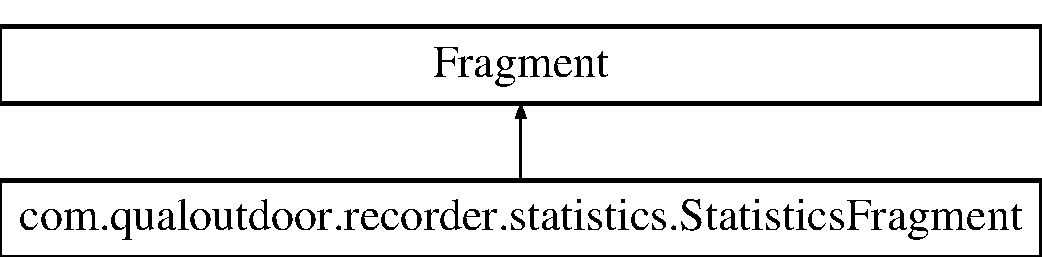
\includegraphics[height=2.000000cm]{classcom_1_1qualoutdoor_1_1recorder_1_1statistics_1_1StatisticsFragment}
\end{center}
\end{figure}
\subsection*{Public Member Functions}
\begin{DoxyCompactItemize}
\item 
\hypertarget{classcom_1_1qualoutdoor_1_1recorder_1_1statistics_1_1StatisticsFragment_ae6e4e41b7d0dc95f59d15c2a0a276f57}{void {\bfseries on\-Create} (Bundle saved\-Instance\-State)}\label{classcom_1_1qualoutdoor_1_1recorder_1_1statistics_1_1StatisticsFragment_ae6e4e41b7d0dc95f59d15c2a0a276f57}

\item 
\hypertarget{classcom_1_1qualoutdoor_1_1recorder_1_1statistics_1_1StatisticsFragment_ac5359d8e9d4bc64beddda84b3bb2aef6}{View {\bfseries on\-Create\-View} (Layout\-Inflater inflater, View\-Group container, Bundle saved\-Instance\-State)}\label{classcom_1_1qualoutdoor_1_1recorder_1_1statistics_1_1StatisticsFragment_ac5359d8e9d4bc64beddda84b3bb2aef6}

\end{DoxyCompactItemize}
\subsection*{Private Attributes}
\begin{DoxyCompactItemize}
\item 
\hyperlink{classcom_1_1qualoutdoor_1_1recorder_1_1statistics_1_1StatisticsPagerAdapter}{Statistics\-Pager\-Adapter} \hyperlink{classcom_1_1qualoutdoor_1_1recorder_1_1statistics_1_1StatisticsFragment_ab412cc69f46b3a557a8a87e08a1639f6}{statistics\-Pager\-Adapter}
\item 
View\-Pager \hyperlink{classcom_1_1qualoutdoor_1_1recorder_1_1statistics_1_1StatisticsFragment_afd41587fab90a4894b03e036dd002525}{m\-View\-Pager}
\end{DoxyCompactItemize}


\subsection{Detailed Description}


Definition at line 12 of file Statistics\-Fragment.\-java.



\subsection{Member Data Documentation}
\hypertarget{classcom_1_1qualoutdoor_1_1recorder_1_1statistics_1_1StatisticsFragment_afd41587fab90a4894b03e036dd002525}{\index{com\-::qualoutdoor\-::recorder\-::statistics\-::\-Statistics\-Fragment@{com\-::qualoutdoor\-::recorder\-::statistics\-::\-Statistics\-Fragment}!m\-View\-Pager@{m\-View\-Pager}}
\index{m\-View\-Pager@{m\-View\-Pager}!com::qualoutdoor::recorder::statistics::StatisticsFragment@{com\-::qualoutdoor\-::recorder\-::statistics\-::\-Statistics\-Fragment}}
\subsubsection[{m\-View\-Pager}]{\setlength{\rightskip}{0pt plus 5cm}View\-Pager com.\-qualoutdoor.\-recorder.\-statistics.\-Statistics\-Fragment.\-m\-View\-Pager\hspace{0.3cm}{\ttfamily [private]}}}\label{classcom_1_1qualoutdoor_1_1recorder_1_1statistics_1_1StatisticsFragment_afd41587fab90a4894b03e036dd002525}
The \hyperlink{}{android.\-support.\-v4.\-view.\-View\-Pager} that will display the object collection. 

Definition at line 29 of file Statistics\-Fragment.\-java.

\hypertarget{classcom_1_1qualoutdoor_1_1recorder_1_1statistics_1_1StatisticsFragment_ab412cc69f46b3a557a8a87e08a1639f6}{\index{com\-::qualoutdoor\-::recorder\-::statistics\-::\-Statistics\-Fragment@{com\-::qualoutdoor\-::recorder\-::statistics\-::\-Statistics\-Fragment}!statistics\-Pager\-Adapter@{statistics\-Pager\-Adapter}}
\index{statistics\-Pager\-Adapter@{statistics\-Pager\-Adapter}!com::qualoutdoor::recorder::statistics::StatisticsFragment@{com\-::qualoutdoor\-::recorder\-::statistics\-::\-Statistics\-Fragment}}
\subsubsection[{statistics\-Pager\-Adapter}]{\setlength{\rightskip}{0pt plus 5cm}{\bf Statistics\-Pager\-Adapter} com.\-qualoutdoor.\-recorder.\-statistics.\-Statistics\-Fragment.\-statistics\-Pager\-Adapter\hspace{0.3cm}{\ttfamily [private]}}}\label{classcom_1_1qualoutdoor_1_1recorder_1_1statistics_1_1StatisticsFragment_ab412cc69f46b3a557a8a87e08a1639f6}
The \hyperlink{}{android.\-support.\-v4.\-view.\-Pager\-Adapter} that will provide fragments representing each object in a collection. We use a \hyperlink{}{android.\-support.\-v4.\-app.\-Fragment\-State\-Pager\-Adapter} derivative, which will destroy and re-\/create fragments as needed, saving and restoring their state in the process. This is important to conserve memory and is a best practice when allowing navigation between objects in a potentially large collection. 

Definition at line 23 of file Statistics\-Fragment.\-java.



The documentation for this class was generated from the following file\-:\begin{DoxyCompactItemize}
\item 
src/com/qualoutdoor/recorder/statistics/Statistics\-Fragment.\-java\end{DoxyCompactItemize}

\hypertarget{classcom_1_1qualoutdoor_1_1recorder_1_1statistics_1_1StatisticsPagerAdapter}{\section{com.\-qualoutdoor.\-recorder.\-statistics.\-Statistics\-Pager\-Adapter Class Reference}
\label{classcom_1_1qualoutdoor_1_1recorder_1_1statistics_1_1StatisticsPagerAdapter}\index{com.\-qualoutdoor.\-recorder.\-statistics.\-Statistics\-Pager\-Adapter@{com.\-qualoutdoor.\-recorder.\-statistics.\-Statistics\-Pager\-Adapter}}
}
Inheritance diagram for com.\-qualoutdoor.\-recorder.\-statistics.\-Statistics\-Pager\-Adapter\-:\begin{figure}[H]
\begin{center}
\leavevmode
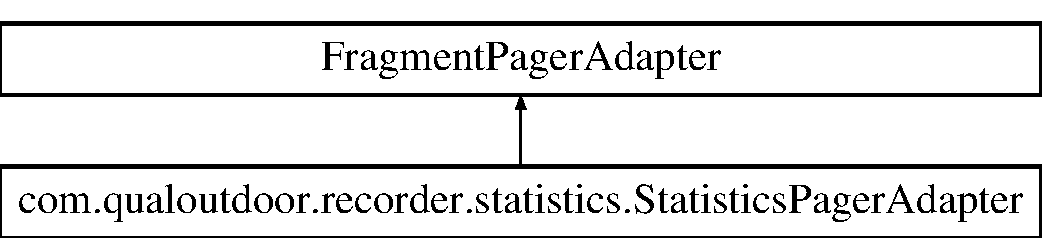
\includegraphics[height=2.000000cm]{classcom_1_1qualoutdoor_1_1recorder_1_1statistics_1_1StatisticsPagerAdapter}
\end{center}
\end{figure}
\subsection*{Public Member Functions}
\begin{DoxyCompactItemize}
\item 
\hypertarget{classcom_1_1qualoutdoor_1_1recorder_1_1statistics_1_1StatisticsPagerAdapter_a5513cfb358b309f7bdde954943f6d8c7}{{\bfseries Statistics\-Pager\-Adapter} (Fragment\-Manager fm)}\label{classcom_1_1qualoutdoor_1_1recorder_1_1statistics_1_1StatisticsPagerAdapter_a5513cfb358b309f7bdde954943f6d8c7}

\item 
\hypertarget{classcom_1_1qualoutdoor_1_1recorder_1_1statistics_1_1StatisticsPagerAdapter_a0ec1243763650f3b047cfde095abb69d}{Fragment {\bfseries get\-Item} (int i)}\label{classcom_1_1qualoutdoor_1_1recorder_1_1statistics_1_1StatisticsPagerAdapter_a0ec1243763650f3b047cfde095abb69d}

\item 
\hypertarget{classcom_1_1qualoutdoor_1_1recorder_1_1statistics_1_1StatisticsPagerAdapter_a9ce894bc0ed657c112da4fec3eb9a982}{int {\bfseries get\-Count} ()}\label{classcom_1_1qualoutdoor_1_1recorder_1_1statistics_1_1StatisticsPagerAdapter_a9ce894bc0ed657c112da4fec3eb9a982}

\item 
\hypertarget{classcom_1_1qualoutdoor_1_1recorder_1_1statistics_1_1StatisticsPagerAdapter_a38adff0033038e48d72f16de75a3bef4}{Char\-Sequence {\bfseries get\-Page\-Title} (int i)}\label{classcom_1_1qualoutdoor_1_1recorder_1_1statistics_1_1StatisticsPagerAdapter_a38adff0033038e48d72f16de75a3bef4}

\end{DoxyCompactItemize}
\subsection*{Private Attributes}
\begin{DoxyCompactItemize}
\item 
Char\-Sequence\mbox{[}$\,$\mbox{]} \hyperlink{classcom_1_1qualoutdoor_1_1recorder_1_1statistics_1_1StatisticsPagerAdapter_a1cc9fe41e3f21712e228dfff867910ef}{fragment\-Titles}
\end{DoxyCompactItemize}
\subsection*{Static Private Attributes}
\begin{DoxyCompactItemize}
\item 
static final int \hyperlink{classcom_1_1qualoutdoor_1_1recorder_1_1statistics_1_1StatisticsPagerAdapter_ab2945fd8047171f62d7424d3e8c40b9b}{C\-E\-L\-L\-\_\-\-I\-N\-F\-O} = 0
\item 
\hypertarget{classcom_1_1qualoutdoor_1_1recorder_1_1statistics_1_1StatisticsPagerAdapter_a0129f5c8b0e2921643fcc7a331d25062}{static final int {\bfseries N\-E\-I\-G\-H\-B\-O\-R} = 1}\label{classcom_1_1qualoutdoor_1_1recorder_1_1statistics_1_1StatisticsPagerAdapter_a0129f5c8b0e2921643fcc7a331d25062}

\item 
\hypertarget{classcom_1_1qualoutdoor_1_1recorder_1_1statistics_1_1StatisticsPagerAdapter_a379ae4d8a688ca9eb90dd1694a64bcc3}{static final int {\bfseries G\-R\-A\-P\-H} = 2}\label{classcom_1_1qualoutdoor_1_1recorder_1_1statistics_1_1StatisticsPagerAdapter_a379ae4d8a688ca9eb90dd1694a64bcc3}

\item 
\hypertarget{classcom_1_1qualoutdoor_1_1recorder_1_1statistics_1_1StatisticsPagerAdapter_adae954e09edc2214d375a1b0c6dd2455}{static final int {\bfseries S\-C\-R\-I\-P\-T\-\_\-\-L\-O\-G\-S} = 3}\label{classcom_1_1qualoutdoor_1_1recorder_1_1statistics_1_1StatisticsPagerAdapter_adae954e09edc2214d375a1b0c6dd2455}

\end{DoxyCompactItemize}


\subsection{Detailed Description}


Definition at line 11 of file Statistics\-Pager\-Adapter.\-java.



\subsection{Member Data Documentation}
\hypertarget{classcom_1_1qualoutdoor_1_1recorder_1_1statistics_1_1StatisticsPagerAdapter_ab2945fd8047171f62d7424d3e8c40b9b}{\index{com\-::qualoutdoor\-::recorder\-::statistics\-::\-Statistics\-Pager\-Adapter@{com\-::qualoutdoor\-::recorder\-::statistics\-::\-Statistics\-Pager\-Adapter}!C\-E\-L\-L\-\_\-\-I\-N\-F\-O@{C\-E\-L\-L\-\_\-\-I\-N\-F\-O}}
\index{C\-E\-L\-L\-\_\-\-I\-N\-F\-O@{C\-E\-L\-L\-\_\-\-I\-N\-F\-O}!com::qualoutdoor::recorder::statistics::StatisticsPagerAdapter@{com\-::qualoutdoor\-::recorder\-::statistics\-::\-Statistics\-Pager\-Adapter}}
\subsubsection[{C\-E\-L\-L\-\_\-\-I\-N\-F\-O}]{\setlength{\rightskip}{0pt plus 5cm}final int com.\-qualoutdoor.\-recorder.\-statistics.\-Statistics\-Pager\-Adapter.\-C\-E\-L\-L\-\_\-\-I\-N\-F\-O = 0\hspace{0.3cm}{\ttfamily [static]}, {\ttfamily [private]}}}\label{classcom_1_1qualoutdoor_1_1recorder_1_1statistics_1_1StatisticsPagerAdapter_ab2945fd8047171f62d7424d3e8c40b9b}
The order of the fragments 

Definition at line 14 of file Statistics\-Pager\-Adapter.\-java.

\hypertarget{classcom_1_1qualoutdoor_1_1recorder_1_1statistics_1_1StatisticsPagerAdapter_a1cc9fe41e3f21712e228dfff867910ef}{\index{com\-::qualoutdoor\-::recorder\-::statistics\-::\-Statistics\-Pager\-Adapter@{com\-::qualoutdoor\-::recorder\-::statistics\-::\-Statistics\-Pager\-Adapter}!fragment\-Titles@{fragment\-Titles}}
\index{fragment\-Titles@{fragment\-Titles}!com::qualoutdoor::recorder::statistics::StatisticsPagerAdapter@{com\-::qualoutdoor\-::recorder\-::statistics\-::\-Statistics\-Pager\-Adapter}}
\subsubsection[{fragment\-Titles}]{\setlength{\rightskip}{0pt plus 5cm}Char\-Sequence \mbox{[}$\,$\mbox{]} com.\-qualoutdoor.\-recorder.\-statistics.\-Statistics\-Pager\-Adapter.\-fragment\-Titles\hspace{0.3cm}{\ttfamily [private]}}}\label{classcom_1_1qualoutdoor_1_1recorder_1_1statistics_1_1StatisticsPagerAdapter_a1cc9fe41e3f21712e228dfff867910ef}
{\bfseries Initial value\-:}
\begin{DoxyCode}
= \{ \textcolor{stringliteral}{"Cell Infos"}, \textcolor{stringliteral}{"Neighbor Cells"},
            \textcolor{stringliteral}{"Graph"}, \textcolor{stringliteral}{"Script Logs"} \}
\end{DoxyCode}
The list of the fragment names 

Definition at line 20 of file Statistics\-Pager\-Adapter.\-java.



The documentation for this class was generated from the following file\-:\begin{DoxyCompactItemize}
\item 
src/com/qualoutdoor/recorder/statistics/Statistics\-Pager\-Adapter.\-java\end{DoxyCompactItemize}

\hypertarget{classcom_1_1qualoutdoor_1_1recorder_1_1telephony_1_1TelephonyBinder}{\section{com.\-qualoutdoor.\-recorder.\-telephony.\-Telephony\-Binder Class Reference}
\label{classcom_1_1qualoutdoor_1_1recorder_1_1telephony_1_1TelephonyBinder}\index{com.\-qualoutdoor.\-recorder.\-telephony.\-Telephony\-Binder@{com.\-qualoutdoor.\-recorder.\-telephony.\-Telephony\-Binder}}
}
Inheritance diagram for com.\-qualoutdoor.\-recorder.\-telephony.\-Telephony\-Binder\-:\begin{figure}[H]
\begin{center}
\leavevmode
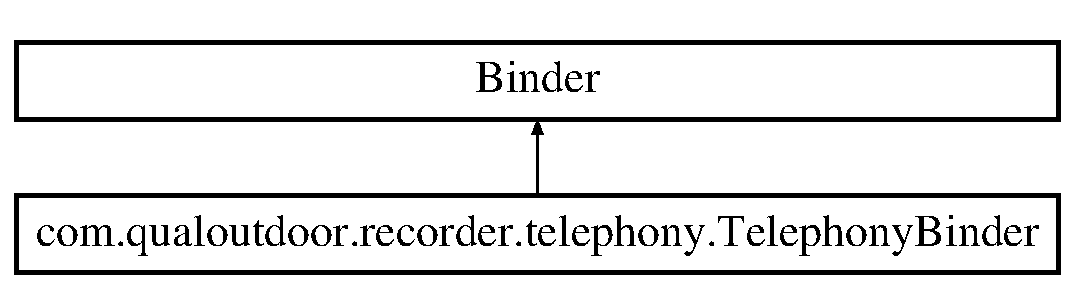
\includegraphics[height=2.000000cm]{classcom_1_1qualoutdoor_1_1recorder_1_1telephony_1_1TelephonyBinder}
\end{center}
\end{figure}
\subsection*{Public Member Functions}
\begin{DoxyCompactItemize}
\item 
\hyperlink{classcom_1_1qualoutdoor_1_1recorder_1_1telephony_1_1TelephonyBinder_afc6a0e5ef46d92a4bf0c9e2ee7df8a33}{Telephony\-Binder} (\hyperlink{classcom_1_1qualoutdoor_1_1recorder_1_1telephony_1_1TelephonyService}{Telephony\-Service} service)
\item 
\hyperlink{classcom_1_1qualoutdoor_1_1recorder_1_1telephony_1_1TelephonyService}{Telephony\-Service} \hyperlink{classcom_1_1qualoutdoor_1_1recorder_1_1telephony_1_1TelephonyBinder_acdfebeb669e80bdf37dec7b4dd65e73b}{get\-Service} ()
\end{DoxyCompactItemize}
\subsection*{Private Attributes}
\begin{DoxyCompactItemize}
\item 
\hyperlink{classcom_1_1qualoutdoor_1_1recorder_1_1telephony_1_1TelephonyService}{Telephony\-Service} \hyperlink{classcom_1_1qualoutdoor_1_1recorder_1_1telephony_1_1TelephonyBinder_a864035a7cb42e95815445f9d6c345492}{my\-Service}
\end{DoxyCompactItemize}


\subsection{Detailed Description}
The local binder for the \hyperlink{classcom_1_1qualoutdoor_1_1recorder_1_1telephony_1_1TelephonyService}{Telephony\-Service}. Caution, this works only if the service and the component binding to it are in the same process. 

Definition at line 9 of file Telephony\-Binder.\-java.



\subsection{Constructor \& Destructor Documentation}
\hypertarget{classcom_1_1qualoutdoor_1_1recorder_1_1telephony_1_1TelephonyBinder_afc6a0e5ef46d92a4bf0c9e2ee7df8a33}{\index{com\-::qualoutdoor\-::recorder\-::telephony\-::\-Telephony\-Binder@{com\-::qualoutdoor\-::recorder\-::telephony\-::\-Telephony\-Binder}!Telephony\-Binder@{Telephony\-Binder}}
\index{Telephony\-Binder@{Telephony\-Binder}!com::qualoutdoor::recorder::telephony::TelephonyBinder@{com\-::qualoutdoor\-::recorder\-::telephony\-::\-Telephony\-Binder}}
\subsubsection[{Telephony\-Binder}]{\setlength{\rightskip}{0pt plus 5cm}com.\-qualoutdoor.\-recorder.\-telephony.\-Telephony\-Binder.\-Telephony\-Binder (
\begin{DoxyParamCaption}
\item[{{\bf Telephony\-Service}}]{service}
\end{DoxyParamCaption}
)}}\label{classcom_1_1qualoutdoor_1_1recorder_1_1telephony_1_1TelephonyBinder_afc6a0e5ef46d92a4bf0c9e2ee7df8a33}
A constructor for the binder to know its service 

Definition at line 15 of file Telephony\-Binder.\-java.



References com.\-qualoutdoor.\-recorder.\-telephony.\-Telephony\-Binder.\-my\-Service.



\subsection{Member Function Documentation}
\hypertarget{classcom_1_1qualoutdoor_1_1recorder_1_1telephony_1_1TelephonyBinder_acdfebeb669e80bdf37dec7b4dd65e73b}{\index{com\-::qualoutdoor\-::recorder\-::telephony\-::\-Telephony\-Binder@{com\-::qualoutdoor\-::recorder\-::telephony\-::\-Telephony\-Binder}!get\-Service@{get\-Service}}
\index{get\-Service@{get\-Service}!com::qualoutdoor::recorder::telephony::TelephonyBinder@{com\-::qualoutdoor\-::recorder\-::telephony\-::\-Telephony\-Binder}}
\subsubsection[{get\-Service}]{\setlength{\rightskip}{0pt plus 5cm}{\bf Telephony\-Service} com.\-qualoutdoor.\-recorder.\-telephony.\-Telephony\-Binder.\-get\-Service (
\begin{DoxyParamCaption}
{}
\end{DoxyParamCaption}
)}}\label{classcom_1_1qualoutdoor_1_1recorder_1_1telephony_1_1TelephonyBinder_acdfebeb669e80bdf37dec7b4dd65e73b}
Get the service that provided this binder 

Definition at line 21 of file Telephony\-Binder.\-java.



References com.\-qualoutdoor.\-recorder.\-telephony.\-Telephony\-Binder.\-my\-Service.



\subsection{Member Data Documentation}
\hypertarget{classcom_1_1qualoutdoor_1_1recorder_1_1telephony_1_1TelephonyBinder_a864035a7cb42e95815445f9d6c345492}{\index{com\-::qualoutdoor\-::recorder\-::telephony\-::\-Telephony\-Binder@{com\-::qualoutdoor\-::recorder\-::telephony\-::\-Telephony\-Binder}!my\-Service@{my\-Service}}
\index{my\-Service@{my\-Service}!com::qualoutdoor::recorder::telephony::TelephonyBinder@{com\-::qualoutdoor\-::recorder\-::telephony\-::\-Telephony\-Binder}}
\subsubsection[{my\-Service}]{\setlength{\rightskip}{0pt plus 5cm}{\bf Telephony\-Service} com.\-qualoutdoor.\-recorder.\-telephony.\-Telephony\-Binder.\-my\-Service\hspace{0.3cm}{\ttfamily [private]}}}\label{classcom_1_1qualoutdoor_1_1recorder_1_1telephony_1_1TelephonyBinder_a864035a7cb42e95815445f9d6c345492}
The service that provided this binder 

Definition at line 12 of file Telephony\-Binder.\-java.



Referenced by com.\-qualoutdoor.\-recorder.\-telephony.\-Telephony\-Binder.\-get\-Service(), and com.\-qualoutdoor.\-recorder.\-telephony.\-Telephony\-Binder.\-Telephony\-Binder().



The documentation for this class was generated from the following file\-:\begin{DoxyCompactItemize}
\item 
src/com/qualoutdoor/recorder/telephony/Telephony\-Binder.\-java\end{DoxyCompactItemize}

\hypertarget{classcom_1_1qualoutdoor_1_1recorder_1_1telephony_1_1TelephonyListener}{\section{com.\-qualoutdoor.\-recorder.\-telephony.\-Telephony\-Listener Class Reference}
\label{classcom_1_1qualoutdoor_1_1recorder_1_1telephony_1_1TelephonyListener}\index{com.\-qualoutdoor.\-recorder.\-telephony.\-Telephony\-Listener@{com.\-qualoutdoor.\-recorder.\-telephony.\-Telephony\-Listener}}
}
\subsection*{Public Member Functions}
\begin{DoxyCompactItemize}
\item 
\hyperlink{classcom_1_1qualoutdoor_1_1recorder_1_1telephony_1_1TelephonyListener_a3d14b9a5603d15201ffef86df42d54f1}{Telephony\-Listener} ()
\item 
void \hyperlink{classcom_1_1qualoutdoor_1_1recorder_1_1telephony_1_1TelephonyListener_a171849910c348658f639011099980d84}{on\-Call\-State\-Changed} (int state, String incoming\-Number)
\item 
void \hyperlink{classcom_1_1qualoutdoor_1_1recorder_1_1telephony_1_1TelephonyListener_ab93e4cd769a3efeedf3d4bd65de8ad15}{on\-Cell\-Info\-Changed} (List$<$ \hyperlink{interfacecom_1_1qualoutdoor_1_1recorder_1_1telephony_1_1ICellInfo}{I\-Cell\-Info} $>$ cell\-Info)
\item 
void \hyperlink{classcom_1_1qualoutdoor_1_1recorder_1_1telephony_1_1TelephonyListener_a671048ccc7d961591b47ce714d660436}{on\-Location\-Changed} (\hyperlink{interfacecom_1_1qualoutdoor_1_1recorder_1_1telephony_1_1ILocation}{I\-Location} location)
\item 
void \hyperlink{classcom_1_1qualoutdoor_1_1recorder_1_1telephony_1_1TelephonyListener_a8b3ff94c072f2d90dc82ae38d390bf62}{on\-Data\-Connection\-State\-Changed} (int state)
\item 
void \hyperlink{classcom_1_1qualoutdoor_1_1recorder_1_1telephony_1_1TelephonyListener_aa5f922c9142ab0e8c933a1953b384269}{on\-Network\-Type\-Changed} (int state, int network\-Type)
\item 
void \hyperlink{classcom_1_1qualoutdoor_1_1recorder_1_1telephony_1_1TelephonyListener_a560acb91a9cb03ad4e4389cc9393c76b}{on\-Signal\-Strengths\-Changed} (\hyperlink{interfacecom_1_1qualoutdoor_1_1recorder_1_1telephony_1_1ISignalStrength}{I\-Signal\-Strength} signal\-Strength)
\end{DoxyCompactItemize}
\subsection*{Static Public Attributes}
\begin{DoxyCompactItemize}
\item 
static final int \hyperlink{classcom_1_1qualoutdoor_1_1recorder_1_1telephony_1_1TelephonyListener_a191d2575b8783002ee3e5d8cbadd6f34}{L\-I\-S\-T\-E\-N\-\_\-\-C\-A\-L\-L\-\_\-\-S\-T\-A\-T\-E} = 8
\item 
static final int \hyperlink{classcom_1_1qualoutdoor_1_1recorder_1_1telephony_1_1TelephonyListener_aa73af11a2afc13c7bfb8ce7e58b45f69}{L\-I\-S\-T\-E\-N\-\_\-\-C\-E\-L\-L\-\_\-\-I\-N\-F\-O} = 1024
\item 
static final int \hyperlink{classcom_1_1qualoutdoor_1_1recorder_1_1telephony_1_1TelephonyListener_a640f1efa08e7e0869335cfc47c3a2124}{L\-I\-S\-T\-E\-N\-\_\-\-D\-A\-T\-A\-\_\-\-C\-O\-N\-N\-E\-C\-T\-I\-O\-N\-\_\-\-S\-T\-A\-T\-E} = 64
\item 
static final int \hyperlink{classcom_1_1qualoutdoor_1_1recorder_1_1telephony_1_1TelephonyListener_a146371faf289ea1d3c019a9da50e6ba2}{L\-I\-S\-T\-E\-N\-\_\-\-L\-O\-C\-A\-T\-I\-O\-N} = 2048
\item 
static final int \hyperlink{classcom_1_1qualoutdoor_1_1recorder_1_1telephony_1_1TelephonyListener_adff97a5ff891440e844b1438c8160ec1}{L\-I\-S\-T\-E\-N\-\_\-\-N\-E\-T\-W\-O\-R\-K\-\_\-\-T\-Y\-P\-E} = 4096
\item 
static final int \hyperlink{classcom_1_1qualoutdoor_1_1recorder_1_1telephony_1_1TelephonyListener_a5d217cc158268f8c01738b0f51e1ce53}{L\-I\-S\-T\-E\-N\-\_\-\-N\-O\-N\-E} = 0
\item 
static final int \hyperlink{classcom_1_1qualoutdoor_1_1recorder_1_1telephony_1_1TelephonyListener_aab3f3a875e74a3b4d6eab7db23683372}{L\-I\-S\-T\-E\-N\-\_\-\-S\-I\-G\-N\-A\-L\-\_\-\-S\-T\-R\-E\-N\-G\-T\-H\-S} = 256
\end{DoxyCompactItemize}


\subsection{Detailed Description}
A listener class for monitoring changes in specific telephony states. Override the methods for the state that you want to receive updates for, and pass your \hyperlink{classcom_1_1qualoutdoor_1_1recorder_1_1telephony_1_1TelephonyListener}{Telephony\-Listener} object, along with bitwise-\/or of the L\-I\-S\-T\-E\-N\-\_\-xxx flags to \hyperlink{interfacecom_1_1qualoutdoor_1_1recorder_1_1telephony_1_1ITelephony_a2bf33ee65f59c2100442f6ba33fac113}{I\-Telephony.\-listen()} 

Definition at line 11 of file Telephony\-Listener.\-java.



\subsection{Constructor \& Destructor Documentation}
\hypertarget{classcom_1_1qualoutdoor_1_1recorder_1_1telephony_1_1TelephonyListener_a3d14b9a5603d15201ffef86df42d54f1}{\index{com\-::qualoutdoor\-::recorder\-::telephony\-::\-Telephony\-Listener@{com\-::qualoutdoor\-::recorder\-::telephony\-::\-Telephony\-Listener}!Telephony\-Listener@{Telephony\-Listener}}
\index{Telephony\-Listener@{Telephony\-Listener}!com::qualoutdoor::recorder::telephony::TelephonyListener@{com\-::qualoutdoor\-::recorder\-::telephony\-::\-Telephony\-Listener}}
\subsubsection[{Telephony\-Listener}]{\setlength{\rightskip}{0pt plus 5cm}com.\-qualoutdoor.\-recorder.\-telephony.\-Telephony\-Listener.\-Telephony\-Listener (
\begin{DoxyParamCaption}
{}
\end{DoxyParamCaption}
)}}\label{classcom_1_1qualoutdoor_1_1recorder_1_1telephony_1_1TelephonyListener_a3d14b9a5603d15201ffef86df42d54f1}
Constructor 

Definition at line 29 of file Telephony\-Listener.\-java.



\subsection{Member Function Documentation}
\hypertarget{classcom_1_1qualoutdoor_1_1recorder_1_1telephony_1_1TelephonyListener_a171849910c348658f639011099980d84}{\index{com\-::qualoutdoor\-::recorder\-::telephony\-::\-Telephony\-Listener@{com\-::qualoutdoor\-::recorder\-::telephony\-::\-Telephony\-Listener}!on\-Call\-State\-Changed@{on\-Call\-State\-Changed}}
\index{on\-Call\-State\-Changed@{on\-Call\-State\-Changed}!com::qualoutdoor::recorder::telephony::TelephonyListener@{com\-::qualoutdoor\-::recorder\-::telephony\-::\-Telephony\-Listener}}
\subsubsection[{on\-Call\-State\-Changed}]{\setlength{\rightskip}{0pt plus 5cm}void com.\-qualoutdoor.\-recorder.\-telephony.\-Telephony\-Listener.\-on\-Call\-State\-Changed (
\begin{DoxyParamCaption}
\item[{int}]{state, }
\item[{String}]{incoming\-Number}
\end{DoxyParamCaption}
)}}\label{classcom_1_1qualoutdoor_1_1recorder_1_1telephony_1_1TelephonyListener_a171849910c348658f639011099980d84}
Callback invoked when device call state changes. 

Definition at line 33 of file Telephony\-Listener.\-java.

\hypertarget{classcom_1_1qualoutdoor_1_1recorder_1_1telephony_1_1TelephonyListener_ab93e4cd769a3efeedf3d4bd65de8ad15}{\index{com\-::qualoutdoor\-::recorder\-::telephony\-::\-Telephony\-Listener@{com\-::qualoutdoor\-::recorder\-::telephony\-::\-Telephony\-Listener}!on\-Cell\-Info\-Changed@{on\-Cell\-Info\-Changed}}
\index{on\-Cell\-Info\-Changed@{on\-Cell\-Info\-Changed}!com::qualoutdoor::recorder::telephony::TelephonyListener@{com\-::qualoutdoor\-::recorder\-::telephony\-::\-Telephony\-Listener}}
\subsubsection[{on\-Cell\-Info\-Changed}]{\setlength{\rightskip}{0pt plus 5cm}void com.\-qualoutdoor.\-recorder.\-telephony.\-Telephony\-Listener.\-on\-Cell\-Info\-Changed (
\begin{DoxyParamCaption}
\item[{List$<$ {\bf I\-Cell\-Info} $>$}]{cell\-Info}
\end{DoxyParamCaption}
)}}\label{classcom_1_1qualoutdoor_1_1recorder_1_1telephony_1_1TelephonyListener_ab93e4cd769a3efeedf3d4bd65de8ad15}
Callback invoked when a observed cell info has changed, or new cells have been added or removed. 

Definition at line 40 of file Telephony\-Listener.\-java.

\hypertarget{classcom_1_1qualoutdoor_1_1recorder_1_1telephony_1_1TelephonyListener_a8b3ff94c072f2d90dc82ae38d390bf62}{\index{com\-::qualoutdoor\-::recorder\-::telephony\-::\-Telephony\-Listener@{com\-::qualoutdoor\-::recorder\-::telephony\-::\-Telephony\-Listener}!on\-Data\-Connection\-State\-Changed@{on\-Data\-Connection\-State\-Changed}}
\index{on\-Data\-Connection\-State\-Changed@{on\-Data\-Connection\-State\-Changed}!com::qualoutdoor::recorder::telephony::TelephonyListener@{com\-::qualoutdoor\-::recorder\-::telephony\-::\-Telephony\-Listener}}
\subsubsection[{on\-Data\-Connection\-State\-Changed}]{\setlength{\rightskip}{0pt plus 5cm}void com.\-qualoutdoor.\-recorder.\-telephony.\-Telephony\-Listener.\-on\-Data\-Connection\-State\-Changed (
\begin{DoxyParamCaption}
\item[{int}]{state}
\end{DoxyParamCaption}
)}}\label{classcom_1_1qualoutdoor_1_1recorder_1_1telephony_1_1TelephonyListener_a8b3ff94c072f2d90dc82ae38d390bf62}
Callback invoked when connection state changes. 

Definition at line 48 of file Telephony\-Listener.\-java.

\hypertarget{classcom_1_1qualoutdoor_1_1recorder_1_1telephony_1_1TelephonyListener_a671048ccc7d961591b47ce714d660436}{\index{com\-::qualoutdoor\-::recorder\-::telephony\-::\-Telephony\-Listener@{com\-::qualoutdoor\-::recorder\-::telephony\-::\-Telephony\-Listener}!on\-Location\-Changed@{on\-Location\-Changed}}
\index{on\-Location\-Changed@{on\-Location\-Changed}!com::qualoutdoor::recorder::telephony::TelephonyListener@{com\-::qualoutdoor\-::recorder\-::telephony\-::\-Telephony\-Listener}}
\subsubsection[{on\-Location\-Changed}]{\setlength{\rightskip}{0pt plus 5cm}void com.\-qualoutdoor.\-recorder.\-telephony.\-Telephony\-Listener.\-on\-Location\-Changed (
\begin{DoxyParamCaption}
\item[{{\bf I\-Location}}]{location}
\end{DoxyParamCaption}
)}}\label{classcom_1_1qualoutdoor_1_1recorder_1_1telephony_1_1TelephonyListener_a671048ccc7d961591b47ce714d660436}
Callback invoked when device location changes. 

Definition at line 44 of file Telephony\-Listener.\-java.

\hypertarget{classcom_1_1qualoutdoor_1_1recorder_1_1telephony_1_1TelephonyListener_aa5f922c9142ab0e8c933a1953b384269}{\index{com\-::qualoutdoor\-::recorder\-::telephony\-::\-Telephony\-Listener@{com\-::qualoutdoor\-::recorder\-::telephony\-::\-Telephony\-Listener}!on\-Network\-Type\-Changed@{on\-Network\-Type\-Changed}}
\index{on\-Network\-Type\-Changed@{on\-Network\-Type\-Changed}!com::qualoutdoor::recorder::telephony::TelephonyListener@{com\-::qualoutdoor\-::recorder\-::telephony\-::\-Telephony\-Listener}}
\subsubsection[{on\-Network\-Type\-Changed}]{\setlength{\rightskip}{0pt plus 5cm}void com.\-qualoutdoor.\-recorder.\-telephony.\-Telephony\-Listener.\-on\-Network\-Type\-Changed (
\begin{DoxyParamCaption}
\item[{int}]{state, }
\item[{int}]{network\-Type}
\end{DoxyParamCaption}
)}}\label{classcom_1_1qualoutdoor_1_1recorder_1_1telephony_1_1TelephonyListener_aa5f922c9142ab0e8c933a1953b384269}
Callback invoked when network type changes. 

Definition at line 52 of file Telephony\-Listener.\-java.

\hypertarget{classcom_1_1qualoutdoor_1_1recorder_1_1telephony_1_1TelephonyListener_a560acb91a9cb03ad4e4389cc9393c76b}{\index{com\-::qualoutdoor\-::recorder\-::telephony\-::\-Telephony\-Listener@{com\-::qualoutdoor\-::recorder\-::telephony\-::\-Telephony\-Listener}!on\-Signal\-Strengths\-Changed@{on\-Signal\-Strengths\-Changed}}
\index{on\-Signal\-Strengths\-Changed@{on\-Signal\-Strengths\-Changed}!com::qualoutdoor::recorder::telephony::TelephonyListener@{com\-::qualoutdoor\-::recorder\-::telephony\-::\-Telephony\-Listener}}
\subsubsection[{on\-Signal\-Strengths\-Changed}]{\setlength{\rightskip}{0pt plus 5cm}void com.\-qualoutdoor.\-recorder.\-telephony.\-Telephony\-Listener.\-on\-Signal\-Strengths\-Changed (
\begin{DoxyParamCaption}
\item[{{\bf I\-Signal\-Strength}}]{signal\-Strength}
\end{DoxyParamCaption}
)}}\label{classcom_1_1qualoutdoor_1_1recorder_1_1telephony_1_1TelephonyListener_a560acb91a9cb03ad4e4389cc9393c76b}
Callback invoked when network signal strengths changes. 

Definition at line 56 of file Telephony\-Listener.\-java.



\subsection{Member Data Documentation}
\hypertarget{classcom_1_1qualoutdoor_1_1recorder_1_1telephony_1_1TelephonyListener_a191d2575b8783002ee3e5d8cbadd6f34}{\index{com\-::qualoutdoor\-::recorder\-::telephony\-::\-Telephony\-Listener@{com\-::qualoutdoor\-::recorder\-::telephony\-::\-Telephony\-Listener}!L\-I\-S\-T\-E\-N\-\_\-\-C\-A\-L\-L\-\_\-\-S\-T\-A\-T\-E@{L\-I\-S\-T\-E\-N\-\_\-\-C\-A\-L\-L\-\_\-\-S\-T\-A\-T\-E}}
\index{L\-I\-S\-T\-E\-N\-\_\-\-C\-A\-L\-L\-\_\-\-S\-T\-A\-T\-E@{L\-I\-S\-T\-E\-N\-\_\-\-C\-A\-L\-L\-\_\-\-S\-T\-A\-T\-E}!com::qualoutdoor::recorder::telephony::TelephonyListener@{com\-::qualoutdoor\-::recorder\-::telephony\-::\-Telephony\-Listener}}
\subsubsection[{L\-I\-S\-T\-E\-N\-\_\-\-C\-A\-L\-L\-\_\-\-S\-T\-A\-T\-E}]{\setlength{\rightskip}{0pt plus 5cm}final int com.\-qualoutdoor.\-recorder.\-telephony.\-Telephony\-Listener.\-L\-I\-S\-T\-E\-N\-\_\-\-C\-A\-L\-L\-\_\-\-S\-T\-A\-T\-E = 8\hspace{0.3cm}{\ttfamily [static]}}}\label{classcom_1_1qualoutdoor_1_1recorder_1_1telephony_1_1TelephonyListener_a191d2575b8783002ee3e5d8cbadd6f34}
Listen for changes to the device call state. 

Definition at line 14 of file Telephony\-Listener.\-java.

\hypertarget{classcom_1_1qualoutdoor_1_1recorder_1_1telephony_1_1TelephonyListener_aa73af11a2afc13c7bfb8ce7e58b45f69}{\index{com\-::qualoutdoor\-::recorder\-::telephony\-::\-Telephony\-Listener@{com\-::qualoutdoor\-::recorder\-::telephony\-::\-Telephony\-Listener}!L\-I\-S\-T\-E\-N\-\_\-\-C\-E\-L\-L\-\_\-\-I\-N\-F\-O@{L\-I\-S\-T\-E\-N\-\_\-\-C\-E\-L\-L\-\_\-\-I\-N\-F\-O}}
\index{L\-I\-S\-T\-E\-N\-\_\-\-C\-E\-L\-L\-\_\-\-I\-N\-F\-O@{L\-I\-S\-T\-E\-N\-\_\-\-C\-E\-L\-L\-\_\-\-I\-N\-F\-O}!com::qualoutdoor::recorder::telephony::TelephonyListener@{com\-::qualoutdoor\-::recorder\-::telephony\-::\-Telephony\-Listener}}
\subsubsection[{L\-I\-S\-T\-E\-N\-\_\-\-C\-E\-L\-L\-\_\-\-I\-N\-F\-O}]{\setlength{\rightskip}{0pt plus 5cm}final int com.\-qualoutdoor.\-recorder.\-telephony.\-Telephony\-Listener.\-L\-I\-S\-T\-E\-N\-\_\-\-C\-E\-L\-L\-\_\-\-I\-N\-F\-O = 1024\hspace{0.3cm}{\ttfamily [static]}}}\label{classcom_1_1qualoutdoor_1_1recorder_1_1telephony_1_1TelephonyListener_aa73af11a2afc13c7bfb8ce7e58b45f69}
Listen for changes to observed cell info. 

Definition at line 16 of file Telephony\-Listener.\-java.

\hypertarget{classcom_1_1qualoutdoor_1_1recorder_1_1telephony_1_1TelephonyListener_a640f1efa08e7e0869335cfc47c3a2124}{\index{com\-::qualoutdoor\-::recorder\-::telephony\-::\-Telephony\-Listener@{com\-::qualoutdoor\-::recorder\-::telephony\-::\-Telephony\-Listener}!L\-I\-S\-T\-E\-N\-\_\-\-D\-A\-T\-A\-\_\-\-C\-O\-N\-N\-E\-C\-T\-I\-O\-N\-\_\-\-S\-T\-A\-T\-E@{L\-I\-S\-T\-E\-N\-\_\-\-D\-A\-T\-A\-\_\-\-C\-O\-N\-N\-E\-C\-T\-I\-O\-N\-\_\-\-S\-T\-A\-T\-E}}
\index{L\-I\-S\-T\-E\-N\-\_\-\-D\-A\-T\-A\-\_\-\-C\-O\-N\-N\-E\-C\-T\-I\-O\-N\-\_\-\-S\-T\-A\-T\-E@{L\-I\-S\-T\-E\-N\-\_\-\-D\-A\-T\-A\-\_\-\-C\-O\-N\-N\-E\-C\-T\-I\-O\-N\-\_\-\-S\-T\-A\-T\-E}!com::qualoutdoor::recorder::telephony::TelephonyListener@{com\-::qualoutdoor\-::recorder\-::telephony\-::\-Telephony\-Listener}}
\subsubsection[{L\-I\-S\-T\-E\-N\-\_\-\-D\-A\-T\-A\-\_\-\-C\-O\-N\-N\-E\-C\-T\-I\-O\-N\-\_\-\-S\-T\-A\-T\-E}]{\setlength{\rightskip}{0pt plus 5cm}final int com.\-qualoutdoor.\-recorder.\-telephony.\-Telephony\-Listener.\-L\-I\-S\-T\-E\-N\-\_\-\-D\-A\-T\-A\-\_\-\-C\-O\-N\-N\-E\-C\-T\-I\-O\-N\-\_\-\-S\-T\-A\-T\-E = 64\hspace{0.3cm}{\ttfamily [static]}}}\label{classcom_1_1qualoutdoor_1_1recorder_1_1telephony_1_1TelephonyListener_a640f1efa08e7e0869335cfc47c3a2124}
Listen for changes to the data connection state (cellular). 

Definition at line 18 of file Telephony\-Listener.\-java.

\hypertarget{classcom_1_1qualoutdoor_1_1recorder_1_1telephony_1_1TelephonyListener_a146371faf289ea1d3c019a9da50e6ba2}{\index{com\-::qualoutdoor\-::recorder\-::telephony\-::\-Telephony\-Listener@{com\-::qualoutdoor\-::recorder\-::telephony\-::\-Telephony\-Listener}!L\-I\-S\-T\-E\-N\-\_\-\-L\-O\-C\-A\-T\-I\-O\-N@{L\-I\-S\-T\-E\-N\-\_\-\-L\-O\-C\-A\-T\-I\-O\-N}}
\index{L\-I\-S\-T\-E\-N\-\_\-\-L\-O\-C\-A\-T\-I\-O\-N@{L\-I\-S\-T\-E\-N\-\_\-\-L\-O\-C\-A\-T\-I\-O\-N}!com::qualoutdoor::recorder::telephony::TelephonyListener@{com\-::qualoutdoor\-::recorder\-::telephony\-::\-Telephony\-Listener}}
\subsubsection[{L\-I\-S\-T\-E\-N\-\_\-\-L\-O\-C\-A\-T\-I\-O\-N}]{\setlength{\rightskip}{0pt plus 5cm}final int com.\-qualoutdoor.\-recorder.\-telephony.\-Telephony\-Listener.\-L\-I\-S\-T\-E\-N\-\_\-\-L\-O\-C\-A\-T\-I\-O\-N = 2048\hspace{0.3cm}{\ttfamily [static]}}}\label{classcom_1_1qualoutdoor_1_1recorder_1_1telephony_1_1TelephonyListener_a146371faf289ea1d3c019a9da50e6ba2}
Listen for changes to the device location 

Definition at line 20 of file Telephony\-Listener.\-java.

\hypertarget{classcom_1_1qualoutdoor_1_1recorder_1_1telephony_1_1TelephonyListener_adff97a5ff891440e844b1438c8160ec1}{\index{com\-::qualoutdoor\-::recorder\-::telephony\-::\-Telephony\-Listener@{com\-::qualoutdoor\-::recorder\-::telephony\-::\-Telephony\-Listener}!L\-I\-S\-T\-E\-N\-\_\-\-N\-E\-T\-W\-O\-R\-K\-\_\-\-T\-Y\-P\-E@{L\-I\-S\-T\-E\-N\-\_\-\-N\-E\-T\-W\-O\-R\-K\-\_\-\-T\-Y\-P\-E}}
\index{L\-I\-S\-T\-E\-N\-\_\-\-N\-E\-T\-W\-O\-R\-K\-\_\-\-T\-Y\-P\-E@{L\-I\-S\-T\-E\-N\-\_\-\-N\-E\-T\-W\-O\-R\-K\-\_\-\-T\-Y\-P\-E}!com::qualoutdoor::recorder::telephony::TelephonyListener@{com\-::qualoutdoor\-::recorder\-::telephony\-::\-Telephony\-Listener}}
\subsubsection[{L\-I\-S\-T\-E\-N\-\_\-\-N\-E\-T\-W\-O\-R\-K\-\_\-\-T\-Y\-P\-E}]{\setlength{\rightskip}{0pt plus 5cm}final int com.\-qualoutdoor.\-recorder.\-telephony.\-Telephony\-Listener.\-L\-I\-S\-T\-E\-N\-\_\-\-N\-E\-T\-W\-O\-R\-K\-\_\-\-T\-Y\-P\-E = 4096\hspace{0.3cm}{\ttfamily [static]}}}\label{classcom_1_1qualoutdoor_1_1recorder_1_1telephony_1_1TelephonyListener_adff97a5ff891440e844b1438c8160ec1}
Listen for changes to the network type 

Definition at line 22 of file Telephony\-Listener.\-java.

\hypertarget{classcom_1_1qualoutdoor_1_1recorder_1_1telephony_1_1TelephonyListener_a5d217cc158268f8c01738b0f51e1ce53}{\index{com\-::qualoutdoor\-::recorder\-::telephony\-::\-Telephony\-Listener@{com\-::qualoutdoor\-::recorder\-::telephony\-::\-Telephony\-Listener}!L\-I\-S\-T\-E\-N\-\_\-\-N\-O\-N\-E@{L\-I\-S\-T\-E\-N\-\_\-\-N\-O\-N\-E}}
\index{L\-I\-S\-T\-E\-N\-\_\-\-N\-O\-N\-E@{L\-I\-S\-T\-E\-N\-\_\-\-N\-O\-N\-E}!com::qualoutdoor::recorder::telephony::TelephonyListener@{com\-::qualoutdoor\-::recorder\-::telephony\-::\-Telephony\-Listener}}
\subsubsection[{L\-I\-S\-T\-E\-N\-\_\-\-N\-O\-N\-E}]{\setlength{\rightskip}{0pt plus 5cm}final int com.\-qualoutdoor.\-recorder.\-telephony.\-Telephony\-Listener.\-L\-I\-S\-T\-E\-N\-\_\-\-N\-O\-N\-E = 0\hspace{0.3cm}{\ttfamily [static]}}}\label{classcom_1_1qualoutdoor_1_1recorder_1_1telephony_1_1TelephonyListener_a5d217cc158268f8c01738b0f51e1ce53}
Stop listening for updates. 

Definition at line 24 of file Telephony\-Listener.\-java.

\hypertarget{classcom_1_1qualoutdoor_1_1recorder_1_1telephony_1_1TelephonyListener_aab3f3a875e74a3b4d6eab7db23683372}{\index{com\-::qualoutdoor\-::recorder\-::telephony\-::\-Telephony\-Listener@{com\-::qualoutdoor\-::recorder\-::telephony\-::\-Telephony\-Listener}!L\-I\-S\-T\-E\-N\-\_\-\-S\-I\-G\-N\-A\-L\-\_\-\-S\-T\-R\-E\-N\-G\-T\-H\-S@{L\-I\-S\-T\-E\-N\-\_\-\-S\-I\-G\-N\-A\-L\-\_\-\-S\-T\-R\-E\-N\-G\-T\-H\-S}}
\index{L\-I\-S\-T\-E\-N\-\_\-\-S\-I\-G\-N\-A\-L\-\_\-\-S\-T\-R\-E\-N\-G\-T\-H\-S@{L\-I\-S\-T\-E\-N\-\_\-\-S\-I\-G\-N\-A\-L\-\_\-\-S\-T\-R\-E\-N\-G\-T\-H\-S}!com::qualoutdoor::recorder::telephony::TelephonyListener@{com\-::qualoutdoor\-::recorder\-::telephony\-::\-Telephony\-Listener}}
\subsubsection[{L\-I\-S\-T\-E\-N\-\_\-\-S\-I\-G\-N\-A\-L\-\_\-\-S\-T\-R\-E\-N\-G\-T\-H\-S}]{\setlength{\rightskip}{0pt plus 5cm}final int com.\-qualoutdoor.\-recorder.\-telephony.\-Telephony\-Listener.\-L\-I\-S\-T\-E\-N\-\_\-\-S\-I\-G\-N\-A\-L\-\_\-\-S\-T\-R\-E\-N\-G\-T\-H\-S = 256\hspace{0.3cm}{\ttfamily [static]}}}\label{classcom_1_1qualoutdoor_1_1recorder_1_1telephony_1_1TelephonyListener_aab3f3a875e74a3b4d6eab7db23683372}
Listen for changes to the network signal strengths (cellular). 

Definition at line 26 of file Telephony\-Listener.\-java.



The documentation for this class was generated from the following file\-:\begin{DoxyCompactItemize}
\item 
src/com/qualoutdoor/recorder/telephony/Telephony\-Listener.\-java\end{DoxyCompactItemize}

\hypertarget{classcom_1_1qualoutdoor_1_1recorder_1_1telephony_1_1TelephonyService}{\section{com.\-qualoutdoor.\-recorder.\-telephony.\-Telephony\-Service Class Reference}
\label{classcom_1_1qualoutdoor_1_1recorder_1_1telephony_1_1TelephonyService}\index{com.\-qualoutdoor.\-recorder.\-telephony.\-Telephony\-Service@{com.\-qualoutdoor.\-recorder.\-telephony.\-Telephony\-Service}}
}
Inheritance diagram for com.\-qualoutdoor.\-recorder.\-telephony.\-Telephony\-Service\-:\begin{figure}[H]
\begin{center}
\leavevmode
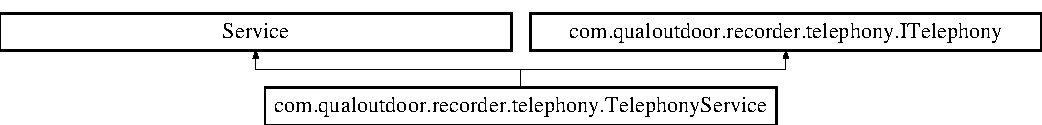
\includegraphics[height=1.681682cm]{classcom_1_1qualoutdoor_1_1recorder_1_1telephony_1_1TelephonyService}
\end{center}
\end{figure}
\subsection*{Public Member Functions}
\begin{DoxyCompactItemize}
\item 
\hypertarget{classcom_1_1qualoutdoor_1_1recorder_1_1telephony_1_1TelephonyService_a103e5234b34bb7dbf1ba8be4a23ac525}{void {\bfseries on\-Create} ()}\label{classcom_1_1qualoutdoor_1_1recorder_1_1telephony_1_1TelephonyService_a103e5234b34bb7dbf1ba8be4a23ac525}

\item 
\hypertarget{classcom_1_1qualoutdoor_1_1recorder_1_1telephony_1_1TelephonyService_a711831c95269c8a1ddf8718e6df105c0}{void {\bfseries on\-Destroy} ()}\label{classcom_1_1qualoutdoor_1_1recorder_1_1telephony_1_1TelephonyService_a711831c95269c8a1ddf8718e6df105c0}

\item 
\hypertarget{classcom_1_1qualoutdoor_1_1recorder_1_1telephony_1_1TelephonyService_af093ee2d853356659960e1a1125e594f}{I\-Binder {\bfseries on\-Bind} (Intent intent)}\label{classcom_1_1qualoutdoor_1_1recorder_1_1telephony_1_1TelephonyService_af093ee2d853356659960e1a1125e594f}

\item 
List$<$ \hyperlink{interfacecom_1_1qualoutdoor_1_1recorder_1_1telephony_1_1ICellInfo}{I\-Cell\-Info} $>$ \hyperlink{classcom_1_1qualoutdoor_1_1recorder_1_1telephony_1_1TelephonyService_a7b9d95b5f6c9b8eb9e970f6c7f254677}{get\-All\-Cell\-Info} ()
\item 
int \hyperlink{classcom_1_1qualoutdoor_1_1recorder_1_1telephony_1_1TelephonyService_ab4452ab5791e52a2a00e7d2ee7626efd}{get\-Call\-State} ()
\item 
int \hyperlink{classcom_1_1qualoutdoor_1_1recorder_1_1telephony_1_1TelephonyService_ab75e2767c592cb1c48ccefcbe075ed1b}{get\-Data\-State} ()
\item 
int \hyperlink{classcom_1_1qualoutdoor_1_1recorder_1_1telephony_1_1TelephonyService_ab5c56c3345271c1146d0d4da90914b01}{get\-Network\-Type} ()
\item 
\hyperlink{interfacecom_1_1qualoutdoor_1_1recorder_1_1telephony_1_1ILocation}{I\-Location} \hyperlink{classcom_1_1qualoutdoor_1_1recorder_1_1telephony_1_1TelephonyService_af3e55e756592010491b87da8927e5cc9}{get\-Location} ()
\item 
\hyperlink{interfacecom_1_1qualoutdoor_1_1recorder_1_1telephony_1_1ISignalStrength}{I\-Signal\-Strength} \hyperlink{classcom_1_1qualoutdoor_1_1recorder_1_1telephony_1_1TelephonyService_a9360c2f3e55992b06c38d26cbf1768c0}{get\-Signal\-Strength} ()
\item 
void \hyperlink{classcom_1_1qualoutdoor_1_1recorder_1_1telephony_1_1TelephonyService_ae688a21a3298fab47e845c0b7ba8065e}{listen} (\hyperlink{classcom_1_1qualoutdoor_1_1recorder_1_1telephony_1_1TelephonyListener}{Telephony\-Listener} listener, int \hyperlink{classcom_1_1qualoutdoor_1_1recorder_1_1telephony_1_1TelephonyService_ab8b427dc82941cff7a38a14300f42f3c}{events})
\item 
void \hyperlink{classcom_1_1qualoutdoor_1_1recorder_1_1telephony_1_1TelephonyService_a8c2446484f717c321902b171161b3dbf}{set\-Minimum\-Refresh\-Rate} (int milliseconds)
\end{DoxyCompactItemize}
\subsection*{Private Attributes}
\begin{DoxyCompactItemize}
\item 
I\-Binder \hyperlink{classcom_1_1qualoutdoor_1_1recorder_1_1telephony_1_1TelephonyService_a1d7f4bd289769acd6c35b25a5ef31aed}{m\-Telephony\-Binder}
\item 
Telephony\-Manager \hyperlink{classcom_1_1qualoutdoor_1_1recorder_1_1telephony_1_1TelephonyService_a81a6850efcbcff0936ed580cb171ba3d}{telephony\-Manager}
\item 
Phone\-State\-Listener \hyperlink{classcom_1_1qualoutdoor_1_1recorder_1_1telephony_1_1TelephonyService_a506be3a4dee76693c315a0e377c506e5}{phone\-State\-Listener}
\item 
\hyperlink{classcom_1_1qualoutdoor_1_1recorder_1_1telephony_1_1CustomSignalStrength}{Custom\-Signal\-Strength} \hyperlink{classcom_1_1qualoutdoor_1_1recorder_1_1telephony_1_1TelephonyService_a52b73496a64d8a0b34d3635a76c5aadf}{signal\-Strength}
\end{DoxyCompactItemize}
\subsection*{Static Private Attributes}
\begin{DoxyCompactItemize}
\item 
static int \hyperlink{classcom_1_1qualoutdoor_1_1recorder_1_1telephony_1_1TelephonyService_ab8b427dc82941cff7a38a14300f42f3c}{events} = Phone\-State\-Listener.\-L\-I\-S\-T\-E\-N\-\_\-\-S\-I\-G\-N\-A\-L\-\_\-\-S\-T\-R\-E\-N\-G\-T\-H\-S
\end{DoxyCompactItemize}
\subsection*{Additional Inherited Members}


\subsection{Detailed Description}
This service is an Android implementation of \hyperlink{interfacecom_1_1qualoutdoor_1_1recorder_1_1telephony_1_1ITelephony}{I\-Telephony}, it uses a Telephony\-Manager to access phone state informations. An app component can bind to it anytime in order to monitor the phone state. 

Definition at line 19 of file Telephony\-Service.\-java.



\subsection{Member Function Documentation}
\hypertarget{classcom_1_1qualoutdoor_1_1recorder_1_1telephony_1_1TelephonyService_a7b9d95b5f6c9b8eb9e970f6c7f254677}{\index{com\-::qualoutdoor\-::recorder\-::telephony\-::\-Telephony\-Service@{com\-::qualoutdoor\-::recorder\-::telephony\-::\-Telephony\-Service}!get\-All\-Cell\-Info@{get\-All\-Cell\-Info}}
\index{get\-All\-Cell\-Info@{get\-All\-Cell\-Info}!com::qualoutdoor::recorder::telephony::TelephonyService@{com\-::qualoutdoor\-::recorder\-::telephony\-::\-Telephony\-Service}}
\subsubsection[{get\-All\-Cell\-Info}]{\setlength{\rightskip}{0pt plus 5cm}List$<${\bf I\-Cell\-Info}$>$ com.\-qualoutdoor.\-recorder.\-telephony.\-Telephony\-Service.\-get\-All\-Cell\-Info (
\begin{DoxyParamCaption}
{}
\end{DoxyParamCaption}
)}}\label{classcom_1_1qualoutdoor_1_1recorder_1_1telephony_1_1TelephonyService_a7b9d95b5f6c9b8eb9e970f6c7f254677}
Returns all the observed cell information including primary and neighboring cells. 

Implements \hyperlink{interfacecom_1_1qualoutdoor_1_1recorder_1_1telephony_1_1ITelephony_ac5f0965e1dfccd7207f49c277593acaa}{com.\-qualoutdoor.\-recorder.\-telephony.\-I\-Telephony}.



Definition at line 71 of file Telephony\-Service.\-java.

\hypertarget{classcom_1_1qualoutdoor_1_1recorder_1_1telephony_1_1TelephonyService_ab4452ab5791e52a2a00e7d2ee7626efd}{\index{com\-::qualoutdoor\-::recorder\-::telephony\-::\-Telephony\-Service@{com\-::qualoutdoor\-::recorder\-::telephony\-::\-Telephony\-Service}!get\-Call\-State@{get\-Call\-State}}
\index{get\-Call\-State@{get\-Call\-State}!com::qualoutdoor::recorder::telephony::TelephonyService@{com\-::qualoutdoor\-::recorder\-::telephony\-::\-Telephony\-Service}}
\subsubsection[{get\-Call\-State}]{\setlength{\rightskip}{0pt plus 5cm}int com.\-qualoutdoor.\-recorder.\-telephony.\-Telephony\-Service.\-get\-Call\-State (
\begin{DoxyParamCaption}
{}
\end{DoxyParamCaption}
)}}\label{classcom_1_1qualoutdoor_1_1recorder_1_1telephony_1_1TelephonyService_ab4452ab5791e52a2a00e7d2ee7626efd}
Returns a constant indicating the call state on the device. 

Implements \hyperlink{interfacecom_1_1qualoutdoor_1_1recorder_1_1telephony_1_1ITelephony_a1b955c3be64a899274bf112d05c8d41a}{com.\-qualoutdoor.\-recorder.\-telephony.\-I\-Telephony}.



Definition at line 78 of file Telephony\-Service.\-java.

\hypertarget{classcom_1_1qualoutdoor_1_1recorder_1_1telephony_1_1TelephonyService_ab75e2767c592cb1c48ccefcbe075ed1b}{\index{com\-::qualoutdoor\-::recorder\-::telephony\-::\-Telephony\-Service@{com\-::qualoutdoor\-::recorder\-::telephony\-::\-Telephony\-Service}!get\-Data\-State@{get\-Data\-State}}
\index{get\-Data\-State@{get\-Data\-State}!com::qualoutdoor::recorder::telephony::TelephonyService@{com\-::qualoutdoor\-::recorder\-::telephony\-::\-Telephony\-Service}}
\subsubsection[{get\-Data\-State}]{\setlength{\rightskip}{0pt plus 5cm}int com.\-qualoutdoor.\-recorder.\-telephony.\-Telephony\-Service.\-get\-Data\-State (
\begin{DoxyParamCaption}
{}
\end{DoxyParamCaption}
)}}\label{classcom_1_1qualoutdoor_1_1recorder_1_1telephony_1_1TelephonyService_ab75e2767c592cb1c48ccefcbe075ed1b}
Returns a constant indicating the data connection state on the device. 

Implements \hyperlink{interfacecom_1_1qualoutdoor_1_1recorder_1_1telephony_1_1ITelephony_ab4135b0c4f01f0169b3a1ea63054b946}{com.\-qualoutdoor.\-recorder.\-telephony.\-I\-Telephony}.



Definition at line 86 of file Telephony\-Service.\-java.

\hypertarget{classcom_1_1qualoutdoor_1_1recorder_1_1telephony_1_1TelephonyService_af3e55e756592010491b87da8927e5cc9}{\index{com\-::qualoutdoor\-::recorder\-::telephony\-::\-Telephony\-Service@{com\-::qualoutdoor\-::recorder\-::telephony\-::\-Telephony\-Service}!get\-Location@{get\-Location}}
\index{get\-Location@{get\-Location}!com::qualoutdoor::recorder::telephony::TelephonyService@{com\-::qualoutdoor\-::recorder\-::telephony\-::\-Telephony\-Service}}
\subsubsection[{get\-Location}]{\setlength{\rightskip}{0pt plus 5cm}{\bf I\-Location} com.\-qualoutdoor.\-recorder.\-telephony.\-Telephony\-Service.\-get\-Location (
\begin{DoxyParamCaption}
{}
\end{DoxyParamCaption}
)}}\label{classcom_1_1qualoutdoor_1_1recorder_1_1telephony_1_1TelephonyService_af3e55e756592010491b87da8927e5cc9}
Returns the most recently observed location 

Implements \hyperlink{interfacecom_1_1qualoutdoor_1_1recorder_1_1telephony_1_1ITelephony_acb95b0c4243cfca3c56776fc0ae3d18e}{com.\-qualoutdoor.\-recorder.\-telephony.\-I\-Telephony}.



Definition at line 102 of file Telephony\-Service.\-java.

\hypertarget{classcom_1_1qualoutdoor_1_1recorder_1_1telephony_1_1TelephonyService_ab5c56c3345271c1146d0d4da90914b01}{\index{com\-::qualoutdoor\-::recorder\-::telephony\-::\-Telephony\-Service@{com\-::qualoutdoor\-::recorder\-::telephony\-::\-Telephony\-Service}!get\-Network\-Type@{get\-Network\-Type}}
\index{get\-Network\-Type@{get\-Network\-Type}!com::qualoutdoor::recorder::telephony::TelephonyService@{com\-::qualoutdoor\-::recorder\-::telephony\-::\-Telephony\-Service}}
\subsubsection[{get\-Network\-Type}]{\setlength{\rightskip}{0pt plus 5cm}int com.\-qualoutdoor.\-recorder.\-telephony.\-Telephony\-Service.\-get\-Network\-Type (
\begin{DoxyParamCaption}
{}
\end{DoxyParamCaption}
)}}\label{classcom_1_1qualoutdoor_1_1recorder_1_1telephony_1_1TelephonyService_ab5c56c3345271c1146d0d4da90914b01}
Returns a constant indicating the network type for the current data connection. 

Implements \hyperlink{interfacecom_1_1qualoutdoor_1_1recorder_1_1telephony_1_1ITelephony_af19331bac8e7317958047a5448274a28}{com.\-qualoutdoor.\-recorder.\-telephony.\-I\-Telephony}.



Definition at line 94 of file Telephony\-Service.\-java.

\hypertarget{classcom_1_1qualoutdoor_1_1recorder_1_1telephony_1_1TelephonyService_a9360c2f3e55992b06c38d26cbf1768c0}{\index{com\-::qualoutdoor\-::recorder\-::telephony\-::\-Telephony\-Service@{com\-::qualoutdoor\-::recorder\-::telephony\-::\-Telephony\-Service}!get\-Signal\-Strength@{get\-Signal\-Strength}}
\index{get\-Signal\-Strength@{get\-Signal\-Strength}!com::qualoutdoor::recorder::telephony::TelephonyService@{com\-::qualoutdoor\-::recorder\-::telephony\-::\-Telephony\-Service}}
\subsubsection[{get\-Signal\-Strength}]{\setlength{\rightskip}{0pt plus 5cm}{\bf I\-Signal\-Strength} com.\-qualoutdoor.\-recorder.\-telephony.\-Telephony\-Service.\-get\-Signal\-Strength (
\begin{DoxyParamCaption}
{}
\end{DoxyParamCaption}
)}}\label{classcom_1_1qualoutdoor_1_1recorder_1_1telephony_1_1TelephonyService_a9360c2f3e55992b06c38d26cbf1768c0}
Return the signal strength of the primary cell 

Implements \hyperlink{interfacecom_1_1qualoutdoor_1_1recorder_1_1telephony_1_1ITelephony_a3454755b99a36692f8ed113144491760}{com.\-qualoutdoor.\-recorder.\-telephony.\-I\-Telephony}.



Definition at line 108 of file Telephony\-Service.\-java.



References com.\-qualoutdoor.\-recorder.\-telephony.\-Telephony\-Service.\-signal\-Strength.

\hypertarget{classcom_1_1qualoutdoor_1_1recorder_1_1telephony_1_1TelephonyService_ae688a21a3298fab47e845c0b7ba8065e}{\index{com\-::qualoutdoor\-::recorder\-::telephony\-::\-Telephony\-Service@{com\-::qualoutdoor\-::recorder\-::telephony\-::\-Telephony\-Service}!listen@{listen}}
\index{listen@{listen}!com::qualoutdoor::recorder::telephony::TelephonyService@{com\-::qualoutdoor\-::recorder\-::telephony\-::\-Telephony\-Service}}
\subsubsection[{listen}]{\setlength{\rightskip}{0pt plus 5cm}void com.\-qualoutdoor.\-recorder.\-telephony.\-Telephony\-Service.\-listen (
\begin{DoxyParamCaption}
\item[{{\bf Telephony\-Listener}}]{listener, }
\item[{int}]{events}
\end{DoxyParamCaption}
)}}\label{classcom_1_1qualoutdoor_1_1recorder_1_1telephony_1_1TelephonyService_ae688a21a3298fab47e845c0b7ba8065e}
Register a listener object to receive notification concerning the specified events type 

Implements \hyperlink{interfacecom_1_1qualoutdoor_1_1recorder_1_1telephony_1_1ITelephony_a2bf33ee65f59c2100442f6ba33fac113}{com.\-qualoutdoor.\-recorder.\-telephony.\-I\-Telephony}.



Definition at line 114 of file Telephony\-Service.\-java.

\hypertarget{classcom_1_1qualoutdoor_1_1recorder_1_1telephony_1_1TelephonyService_a8c2446484f717c321902b171161b3dbf}{\index{com\-::qualoutdoor\-::recorder\-::telephony\-::\-Telephony\-Service@{com\-::qualoutdoor\-::recorder\-::telephony\-::\-Telephony\-Service}!set\-Minimum\-Refresh\-Rate@{set\-Minimum\-Refresh\-Rate}}
\index{set\-Minimum\-Refresh\-Rate@{set\-Minimum\-Refresh\-Rate}!com::qualoutdoor::recorder::telephony::TelephonyService@{com\-::qualoutdoor\-::recorder\-::telephony\-::\-Telephony\-Service}}
\subsubsection[{set\-Minimum\-Refresh\-Rate}]{\setlength{\rightskip}{0pt plus 5cm}void com.\-qualoutdoor.\-recorder.\-telephony.\-Telephony\-Service.\-set\-Minimum\-Refresh\-Rate (
\begin{DoxyParamCaption}
\item[{int}]{milliseconds}
\end{DoxyParamCaption}
)}}\label{classcom_1_1qualoutdoor_1_1recorder_1_1telephony_1_1TelephonyService_a8c2446484f717c321902b171161b3dbf}
Set the minimum refresh rate for non event-\/driven data like All\-Cell\-Infos. These data can't be monitored through a listener, so they need to be refreshed manually by requesting the data provider at a fixed rate. 

Implements \hyperlink{interfacecom_1_1qualoutdoor_1_1recorder_1_1telephony_1_1ITelephony_aaa52e62dfb4607e2f871e3ad0daeba23}{com.\-qualoutdoor.\-recorder.\-telephony.\-I\-Telephony}.



Definition at line 120 of file Telephony\-Service.\-java.



\subsection{Member Data Documentation}
\hypertarget{classcom_1_1qualoutdoor_1_1recorder_1_1telephony_1_1TelephonyService_ab8b427dc82941cff7a38a14300f42f3c}{\index{com\-::qualoutdoor\-::recorder\-::telephony\-::\-Telephony\-Service@{com\-::qualoutdoor\-::recorder\-::telephony\-::\-Telephony\-Service}!events@{events}}
\index{events@{events}!com::qualoutdoor::recorder::telephony::TelephonyService@{com\-::qualoutdoor\-::recorder\-::telephony\-::\-Telephony\-Service}}
\subsubsection[{events}]{\setlength{\rightskip}{0pt plus 5cm}int com.\-qualoutdoor.\-recorder.\-telephony.\-Telephony\-Service.\-events = Phone\-State\-Listener.\-L\-I\-S\-T\-E\-N\-\_\-\-S\-I\-G\-N\-A\-L\-\_\-\-S\-T\-R\-E\-N\-G\-T\-H\-S\hspace{0.3cm}{\ttfamily [static]}, {\ttfamily [private]}}}\label{classcom_1_1qualoutdoor_1_1recorder_1_1telephony_1_1TelephonyService_ab8b427dc82941cff7a38a14300f42f3c}
The events the phone state listener is monitoring 

Definition at line 35 of file Telephony\-Service.\-java.

\hypertarget{classcom_1_1qualoutdoor_1_1recorder_1_1telephony_1_1TelephonyService_a1d7f4bd289769acd6c35b25a5ef31aed}{\index{com\-::qualoutdoor\-::recorder\-::telephony\-::\-Telephony\-Service@{com\-::qualoutdoor\-::recorder\-::telephony\-::\-Telephony\-Service}!m\-Telephony\-Binder@{m\-Telephony\-Binder}}
\index{m\-Telephony\-Binder@{m\-Telephony\-Binder}!com::qualoutdoor::recorder::telephony::TelephonyService@{com\-::qualoutdoor\-::recorder\-::telephony\-::\-Telephony\-Service}}
\subsubsection[{m\-Telephony\-Binder}]{\setlength{\rightskip}{0pt plus 5cm}I\-Binder com.\-qualoutdoor.\-recorder.\-telephony.\-Telephony\-Service.\-m\-Telephony\-Binder\hspace{0.3cm}{\ttfamily [private]}}}\label{classcom_1_1qualoutdoor_1_1recorder_1_1telephony_1_1TelephonyService_a1d7f4bd289769acd6c35b25a5ef31aed}
The interface binder for this service 

Definition at line 22 of file Telephony\-Service.\-java.

\hypertarget{classcom_1_1qualoutdoor_1_1recorder_1_1telephony_1_1TelephonyService_a506be3a4dee76693c315a0e377c506e5}{\index{com\-::qualoutdoor\-::recorder\-::telephony\-::\-Telephony\-Service@{com\-::qualoutdoor\-::recorder\-::telephony\-::\-Telephony\-Service}!phone\-State\-Listener@{phone\-State\-Listener}}
\index{phone\-State\-Listener@{phone\-State\-Listener}!com::qualoutdoor::recorder::telephony::TelephonyService@{com\-::qualoutdoor\-::recorder\-::telephony\-::\-Telephony\-Service}}
\subsubsection[{phone\-State\-Listener}]{\setlength{\rightskip}{0pt plus 5cm}Phone\-State\-Listener com.\-qualoutdoor.\-recorder.\-telephony.\-Telephony\-Service.\-phone\-State\-Listener\hspace{0.3cm}{\ttfamily [private]}}}\label{classcom_1_1qualoutdoor_1_1recorder_1_1telephony_1_1TelephonyService_a506be3a4dee76693c315a0e377c506e5}
{\bfseries Initial value\-:}
\begin{DoxyCode}
= \textcolor{keyword}{new} PhoneStateListener() \{        
        @Override
        \textcolor{keyword}{public} \textcolor{keywordtype}{void} onSignalStrengthsChanged(SignalStrength ss) \{
            signalStrength.setSignalStrength(ss);
            super.onSignalStrengthsChanged(ss);
        \}
    \}
\end{DoxyCode}
The Android phone state listener 

Definition at line 27 of file Telephony\-Service.\-java.

\hypertarget{classcom_1_1qualoutdoor_1_1recorder_1_1telephony_1_1TelephonyService_a52b73496a64d8a0b34d3635a76c5aadf}{\index{com\-::qualoutdoor\-::recorder\-::telephony\-::\-Telephony\-Service@{com\-::qualoutdoor\-::recorder\-::telephony\-::\-Telephony\-Service}!signal\-Strength@{signal\-Strength}}
\index{signal\-Strength@{signal\-Strength}!com::qualoutdoor::recorder::telephony::TelephonyService@{com\-::qualoutdoor\-::recorder\-::telephony\-::\-Telephony\-Service}}
\subsubsection[{signal\-Strength}]{\setlength{\rightskip}{0pt plus 5cm}{\bf Custom\-Signal\-Strength} com.\-qualoutdoor.\-recorder.\-telephony.\-Telephony\-Service.\-signal\-Strength\hspace{0.3cm}{\ttfamily [private]}}}\label{classcom_1_1qualoutdoor_1_1recorder_1_1telephony_1_1TelephonyService_a52b73496a64d8a0b34d3635a76c5aadf}
The current signal strength value 

Definition at line 38 of file Telephony\-Service.\-java.



Referenced by com.\-qualoutdoor.\-recorder.\-telephony.\-Telephony\-Service.\-get\-Signal\-Strength().

\hypertarget{classcom_1_1qualoutdoor_1_1recorder_1_1telephony_1_1TelephonyService_a81a6850efcbcff0936ed580cb171ba3d}{\index{com\-::qualoutdoor\-::recorder\-::telephony\-::\-Telephony\-Service@{com\-::qualoutdoor\-::recorder\-::telephony\-::\-Telephony\-Service}!telephony\-Manager@{telephony\-Manager}}
\index{telephony\-Manager@{telephony\-Manager}!com::qualoutdoor::recorder::telephony::TelephonyService@{com\-::qualoutdoor\-::recorder\-::telephony\-::\-Telephony\-Service}}
\subsubsection[{telephony\-Manager}]{\setlength{\rightskip}{0pt plus 5cm}Telephony\-Manager com.\-qualoutdoor.\-recorder.\-telephony.\-Telephony\-Service.\-telephony\-Manager\hspace{0.3cm}{\ttfamily [private]}}}\label{classcom_1_1qualoutdoor_1_1recorder_1_1telephony_1_1TelephonyService_a81a6850efcbcff0936ed580cb171ba3d}
An instance of Telephony\-Manager 

Definition at line 25 of file Telephony\-Service.\-java.



The documentation for this class was generated from the following file\-:\begin{DoxyCompactItemize}
\item 
src/com/qualoutdoor/recorder/telephony/Telephony\-Service.\-java\end{DoxyCompactItemize}

\hypertarget{classcom_1_1qualoutdoor_1_1recorder_1_1telephony_1_1TelephonyServiceConnection}{\section{com.\-qualoutdoor.\-recorder.\-telephony.\-Telephony\-Service\-Connection Class Reference}
\label{classcom_1_1qualoutdoor_1_1recorder_1_1telephony_1_1TelephonyServiceConnection}\index{com.\-qualoutdoor.\-recorder.\-telephony.\-Telephony\-Service\-Connection@{com.\-qualoutdoor.\-recorder.\-telephony.\-Telephony\-Service\-Connection}}
}
Inheritance diagram for com.\-qualoutdoor.\-recorder.\-telephony.\-Telephony\-Service\-Connection\-:\begin{figure}[H]
\begin{center}
\leavevmode
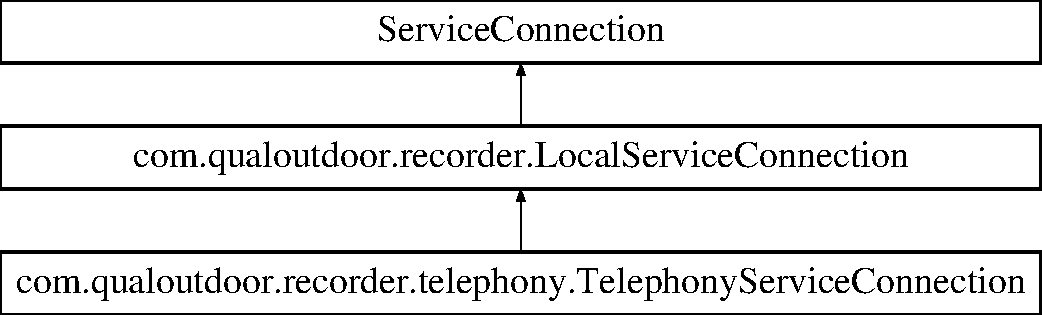
\includegraphics[height=3.000000cm]{classcom_1_1qualoutdoor_1_1recorder_1_1telephony_1_1TelephonyServiceConnection}
\end{center}
\end{figure}
\subsection*{Public Member Functions}
\begin{DoxyCompactItemize}
\item 
\hypertarget{classcom_1_1qualoutdoor_1_1recorder_1_1telephony_1_1TelephonyServiceConnection_acb4ff9183c7f4b7b5f5938a35f97f6c8}{void {\bfseries on\-Service\-Connected} (Component\-Name service\-Name, I\-Binder binder)}\label{classcom_1_1qualoutdoor_1_1recorder_1_1telephony_1_1TelephonyServiceConnection_acb4ff9183c7f4b7b5f5938a35f97f6c8}

\item 
\hyperlink{classcom_1_1qualoutdoor_1_1recorder_1_1telephony_1_1TelephonyService}{Telephony\-Service} \hyperlink{classcom_1_1qualoutdoor_1_1recorder_1_1telephony_1_1TelephonyServiceConnection_ab8017196e7585698b32d6d6766c39f9d}{get\-Service} ()
\end{DoxyCompactItemize}
\subsection*{Private Attributes}
\begin{DoxyCompactItemize}
\item 
\hyperlink{classcom_1_1qualoutdoor_1_1recorder_1_1telephony_1_1TelephonyService}{Telephony\-Service} \hyperlink{classcom_1_1qualoutdoor_1_1recorder_1_1telephony_1_1TelephonyServiceConnection_a209be452896315097a33acbe55d27519}{service}
\end{DoxyCompactItemize}
\subsection*{Additional Inherited Members}


\subsection{Detailed Description}
An implementation for a local Service\-Connection to the \hyperlink{classcom_1_1qualoutdoor_1_1recorder_1_1telephony_1_1TelephonyService}{Telephony\-Service}. Caution \-: this necessitate the binder to be cast into \hyperlink{classcom_1_1qualoutdoor_1_1recorder_1_1telephony_1_1TelephonyBinder}{Telephony\-Binder} on connection. This works because our services belong to the same process. 

Definition at line 14 of file Telephony\-Service\-Connection.\-java.



\subsection{Member Function Documentation}
\hypertarget{classcom_1_1qualoutdoor_1_1recorder_1_1telephony_1_1TelephonyServiceConnection_ab8017196e7585698b32d6d6766c39f9d}{\index{com\-::qualoutdoor\-::recorder\-::telephony\-::\-Telephony\-Service\-Connection@{com\-::qualoutdoor\-::recorder\-::telephony\-::\-Telephony\-Service\-Connection}!get\-Service@{get\-Service}}
\index{get\-Service@{get\-Service}!com::qualoutdoor::recorder::telephony::TelephonyServiceConnection@{com\-::qualoutdoor\-::recorder\-::telephony\-::\-Telephony\-Service\-Connection}}
\subsubsection[{get\-Service}]{\setlength{\rightskip}{0pt plus 5cm}{\bf Telephony\-Service} com.\-qualoutdoor.\-recorder.\-telephony.\-Telephony\-Service\-Connection.\-get\-Service (
\begin{DoxyParamCaption}
{}
\end{DoxyParamCaption}
)}}\label{classcom_1_1qualoutdoor_1_1recorder_1_1telephony_1_1TelephonyServiceConnection_ab8017196e7585698b32d6d6766c39f9d}
Get the binder 

Definition at line 33 of file Telephony\-Service\-Connection.\-java.



References com.\-qualoutdoor.\-recorder.\-telephony.\-Telephony\-Service\-Connection.\-service.



\subsection{Member Data Documentation}
\hypertarget{classcom_1_1qualoutdoor_1_1recorder_1_1telephony_1_1TelephonyServiceConnection_a209be452896315097a33acbe55d27519}{\index{com\-::qualoutdoor\-::recorder\-::telephony\-::\-Telephony\-Service\-Connection@{com\-::qualoutdoor\-::recorder\-::telephony\-::\-Telephony\-Service\-Connection}!service@{service}}
\index{service@{service}!com::qualoutdoor::recorder::telephony::TelephonyServiceConnection@{com\-::qualoutdoor\-::recorder\-::telephony\-::\-Telephony\-Service\-Connection}}
\subsubsection[{service}]{\setlength{\rightskip}{0pt plus 5cm}{\bf Telephony\-Service} com.\-qualoutdoor.\-recorder.\-telephony.\-Telephony\-Service\-Connection.\-service\hspace{0.3cm}{\ttfamily [private]}}}\label{classcom_1_1qualoutdoor_1_1recorder_1_1telephony_1_1TelephonyServiceConnection_a209be452896315097a33acbe55d27519}
The telephony service we connected to 

Definition at line 18 of file Telephony\-Service\-Connection.\-java.



Referenced by com.\-qualoutdoor.\-recorder.\-telephony.\-Telephony\-Service\-Connection.\-get\-Service().



The documentation for this class was generated from the following file\-:\begin{DoxyCompactItemize}
\item 
src/com/qualoutdoor/recorder/telephony/Telephony\-Service\-Connection.\-java\end{DoxyCompactItemize}

%--- End generated contents ---

% Index
\newpage
\phantomsection
\addcontentsline{toc}{chapter}{Index}
\printindex

\end{document}
